% !TEX root = ../geom_autistic_intro.tex
\chapter{Category Theory I}


\section{Categories}

The language of category theory is extremely useful throughout all modern mathematics, but historically it came out of developments in algebraic topology and geometry. Here we try to give a short but intuitive introduction that is focused on ``unlearning'' certain bad habits from traditional mathematics and pushing the reader towards this higher-level way of thinking, which will come in very handy for us later in geometry and group theory. For a more comprehensive introduction for beginners see for example \cite{Leinster, Perrone}.


\begin{defn}[Categories]
    A category\index{Category} $\mathcal{C}$ consists of
    \begin{enumerate}
    \item A class $\ob(\mathcal{C})$ of \emph{objects};
    \item For any $X,Y\in\ob(\mathcal{C})$ there is a set $\mor_{\mathcal{C}}(X,Y)$ (also denoted by $\Hom_{\mathcal{C}}(X,Y)$) of \emph{morphisms}\index{Morphism} (arrows) from $X$ to $Y$ with the following properties:
    \begin{enumerate}
    \item The set of morphisms is closed under \emph{composition}: $\forall f\in\mor(A,B)$
    and $\forall g\in\mor(B,C)$, $\exists h=fg=g\circ f\in\mor(A,C)$.
    \item The composition is associative, $\left(fg\right)h=f\left(gh\right)$.
    \item There is an identity morphism for every object: $\forall A\in\ob(\mathcal{C})$
    $\exists\,\id_{A}\in\mor(A,A)$ such that for any morphisms $f,g$ with
    appropriate domains and codomains, $\id_{A}f=f$ and $g\,\id_{A}=g$.
    \end{enumerate}
    \end{enumerate}
    The set $\mor(A,A)=\Hom(A,A)$ is also denoted $\End(A,A)$ or just $\End(A)$, its elements are called \emph{endomorphisms}\index{Endomorphism} of $A$.
\end{defn}

Notice how the notation $fg$ for the composition where $f$ acts first and $g$ second is more natural for category theory than it is for set theory, because we usually don't refer to arguments of functions here, which means that we'll never have to write strange-looking formulas like $(fg)(x)=g(f(x))$. In the cases where we do need arguments, we will use the set-theoretical notation $g\circ f$. We will always use the set-theoretical notation outside of this section on categories.

A category can be visualized as a directed graph with the vertices
being the objects of the category and the arrows being the morphisms.
\begin{example}
\begin{enumerate}
    \item A category with no objects is called the empty, or trivial, category: $\calC=\varnothing$.
    \item A category with only identity morphisms is called \emph{discrete}.
    \item A category with only one object is called \emph{monoidal}.
\end{enumerate}
    
\end{example}

\begin{example}
    The most basic example of a large category is the category $\mathsf{Set}$\index{Category!of sets},
    whose objects are all sets and the morphisms are all maps between
    sets, i.e., $\mor\left(A,B\right)=\mathrm{Map}\left(A,B\right)$. 

    One \emph{subcategory} of $\mathsf{Set}$ is $\mathsf{FinSet}$,
    i.e., the category of finite sets. $\mathsf{FinSet}$ is a \emph{full
    subcategory} of $\mathsf{Set}$, meaning that $\mor_{\mathsf{FinSet}}(A,B)=\mor_{\mathsf{Set}}(A,B)$.
    In other words, a full subcategory is a subcategory in which only
    the class of objects is truncated and not the sets of morphisms.
\end{example}
%
\begin{example}
    One can truncate the set of morphisms in $\mathsf{Set}$ to obtain
    the categories $\mathsf{Bij}$, $\mathsf{Surj}$, $\mathsf{Inj}$,
    where the morphisms are now bijections, surjections and injections,
    respectively.
\end{example}
%
\begin{example}
    We can also consider $\mathsf{Set}_{\bullet}$ \index{Category!of pointed sets}, the category of ``pointed
    sets''. The objects of the category are doubles $(A,x)$ where $A$
    is a set and $x\in A$ is an element of the set (a ``basepoint'').
    The morphisms $\mor((A,x),(B,y))$ are restricted to those maps $f:A\rightarrow B$
    such that $f(x)=y$, i.e., maps that preserve basepoints.
\end{example}
%
\begin{example}
A generalization of $\mathsf{Set}_{\bullet}$ is the category $\mathsf{SetPair}$\index{Category!of set pairs}
whose objects are pairs $(A,B)$ where $A$ is a set and $B\subset A$.
A morphism $f:(A,B)\rightarrow(C,D)$ must preserve this structure
in the sense that $f(B)\subset D$.
\end{example}
%
\begin{example}[Dual Category]
For any category $\mathcal{C}$ one can define its \emph{dual category}\index{Category!dual}
$\mathcal{C}^{\ast}$ by
\begin{align}
    \ob\left(\mathcal{C}^{\ast}\right) & =\ob\left(\mathcal{C}\right),\nonumber \\
    \mor_{\mathcal{C}^{\ast}}\left(A,B\right) & =\mor_{\mathcal{C}}\left(B,A\right).
\end{align}
In most cases, duals of categories are very difficult to interpret
in any other way than directed graphs. For instance, the dual of $\mathsf{Set}$
has $\mathrm{Mor}_{\mathsf{Set}^{\ast}}\left(\left\{ 1,2\right\} ,\left\{ 1\right\} \right)=\mathrm{Map}\left(\left\{ 1\right\} ,\left\{ 1,2\right\} \right)=\left\{ f_{1},f_{2}\right\} $,
but there aren't two maps from $\left\{ 1,2\right\} $ to $\left\{ 1\right\} $!
Thus the arrows in $\mathsf{Set}^{\ast}$ cannot be interpreted as
maps between sets.
\end{example}





\section{Functors}

We can now construct ``maps'' from categories to categories.
Crucially, we want these maps to preserve as much of the categorical
structure as possible, which is why they have to act not only on objects,
but also on morphisms, in a consistent way.
\begin{defn}[Functors]
    A functor\index{Functor} $F:\mathcal{C}\rightarrow\mathcal{D}$ is a correspondence
    between two categories $\mathcal{C}$ and $\mathcal{D}$ with the
    following properties 
    \begin{enumerate}
        \item $\forall A\in\ob(\mathcal{C})$, $F(A)\in\ob(\mathcal{D})$.
        \item $F$ maps objects to objects, \emph{and} morphisms between objects to
        morphisms between their images:
        \begin{equation}
            \forall f\in\mor_{\mathcal{C}}(A,B),\quad F(f)\in\begin{cases}
            \mor_{\mathcal{D}}(F(A),F(B)), & \text{if \emph{covariant} functor},\\
            \mor_{\mathcal{D}}(F(B),F(A)), & \text{if \emph{contravariant} functor}.
            \end{cases}
        \end{equation}
        
        \item $F$ respects compositions: $\forall~A\in\ob(\mathcal{C})$ we have $F(\id_{A})=\id_{F(A)}$
        and
        \begin{equation}
            F(fg)=\begin{cases}
            F(f)F(g), & \text{if covariant},\\
            F(g)F(f), & \text{if contravariant}.
            \end{cases}
        \end{equation}
    \end{enumerate}
    Covariant functors can be thought of as functors that preserve the direction
    of arrows between objects while contravariant functors reverse the
    arrows.
\end{defn}

The definition of a (covariant) functor is set up in such a way that any sequence of morphisms $A_1\overset{f_1}{\to}A_2\to\cdots\overset{f_n}\to A_{n+1}$ (or simply $f_1f_2\cdots f_n$) in $\mathcal{C}$ is mapped to exactly one morphism $F(f_1)F(f_2)\cdots F(f_n)$ in $\mathcal{D}$. This seemingly trivial property has incredibly deep implications. Represented as a diagram for the case $n=2$, this property looks like this:
\begin{equation}
    \begin{tikzcd}[column sep=small, every matrix/.append style={name=m},   
    execute at end picture={\draw [<-] ([xshift=0em,yshift=.5em]m-2-2.north) arc[start angle=-90,delta angle=270,radius=0.25cm];}]
    F(A_1) \arrow[rr, "F(f_1f_2)"] \arrow[dr, "F(f_1)", swap] & & F(A_3)\\
    & F(A_2)  \arrow[ru, "F(f_2)"'] & 
    \end{tikzcd}
\end{equation}
The circular arrow here indicates that the composition of morphism along any path in this triangle must give the same morphism, i.e., precisely that $F(f_1f_2)=F(f_1)F(f_2)$. When this holds, we say that ``the diagram commutes''. Now suppose $A_3=A_1$ and $f_1=f_2^{-1}$ is an isomorphism between $A_1$ and $A_2$. Then for any functor $F$, not only is it true that $F(\mathrm{id}_{A_1})$ is still an identity morphism, but also that $F(f_1)$ is still an isomorphism, since $F(f_1)F(f_2)=\mathrm{id}_{F(A_1)}$ and $F(f_2)F(f_1)=\mathrm{id}_{F(A_2)}$. Intuitively, this means that \emph{the definition of $F$ itself cannot use any information contained in the objects of $\mathcal{C}$ that is not preserved by isomorphisms}. 

\begin{example}[Non-examples of functors]
    Some common constructions are not functors. For example, for a set $X$ one can define the group $\mathrm{Aut}(X)$ of bijections (permutations) $X\to X$. This is not a functor because there is no nontrivial way to define its action on maps (the trivial way would be to send everything to the identity map).

    Similarly, the monoid (same as a group but without inversion) $\mathrm{End}(X)$ of endomorphisms (i.e., all maps $X\to X$) is also not functorial in $X$.
\end{example}


% \begin{example}
%     Consider once again the category $\mathsf{Set}$. While sets consist of individual elements (numbers, animals, particles...), we all know intuitively that set theory doesn't care about what these elements are, and no element in a given set is more ``special'' than any other one, i.e., two sets ``really'' differ only if there are no bijections between them. Category theory helps us formalize this intuition very easily. Consider the map $F:\mathrm{Ob}(\mathsf{Set})\to \mathrm{Ob}(\mathsf{Set})$ which takes a set and returns some arbitrarily pre-chosen element of that set as a singleton, i.e., $X\mapsto \{x_0\}$ where $x_0\in X$. We would like to establish whether it's possible to extend this $F$ to a functor by defining its action on morphisms, i.e., maps between sets. It is obvious that there is only one potential way to define this action: if $f\in \mathrm{Map}(X,Y)$ then $F(f)$ has to be the unique map from $\{x_0\}$ to $\{y_0\}$. 
    
%     Does this respect the composition property of functors? At first it might seem that the answer is yes: there is always only one map between two singletons, so any equality of the form $F(f_1f_2)=F(f_1)F(f_2)$ is inevitably true.
% \end{example}

The word ``functorial'' is a general adjective that expresses the idea
that many useful constructions in mathematics respect morphisms. Very
roughly, this ``principle of naturality'' can be stated as: 
\begin{gather*}
    \boxed{\begin{array}{c}
    \text{Isomorphic inputs must produce isomorphic outputs.}\\
    \text{In particular, all constructions should not give preference to any}\\ \text{specific representatives of isomorphism classes,}\\
    \text{i.e., they must be \emph{natural}.}
    \end{array}}
\end{gather*}
Looking ahead, an even deeper generalization of this principle will arise when we go up to the level of \emph{morphisms between functors} (called natural transformations).

\begin{example}[Hom-functors]\label{hom-functor example}
    \label{Representable functors}\index{Functor!hom-} One can always construct a functor
    from any category $\mathcal{C}$ to $\mathsf{Set}$, as in the following
    example: for a fixed object $A\in\ob(\mathcal{C})$ consider the quantity
    \begin{equation}
    h^{A}(\_)=\mor_{\mathcal{C}}(A,\_),
    \end{equation}
    where the $\_$ is where the argument of $h^{A}$ goes, i.e., $h_{A}(B)=\mor_{\mathcal{C}}(A,B)$.
    Since the morphisms between any two objects by definition form a set,
    $h^{A}$ is a map from $\ob(\mathcal{C})$ to $\ob(\mathsf{Set})$.
    Can we extend $h^{A}$ to a functor by defining a correspondence between
    morphisms? The answer is yes, and here's how.

    Consider a morphism $f:B\rightarrow C$ in the category $\mathcal{C}$.
    We require correspondingly a map $h^{A}(f):h^{A}(B)\rightarrow h^{A}(C)$.
    $h^{A}(B)$ is the set of maps from $A$ to $B$ and $h^{A}(C)$ is
    the set of maps from $A$ to $C$. Hence, what we require is the following:
    Given a map from $B$ to $C$, how do we transform a map $g:A\rightarrow B$
    into a map from $A$ to $C$? The answer is composition, of course! Hence the map $h^{A}(f)$ acts on $g$ by the action
    \begin{equation}
    h^{A}(f)(g)=gf=f\circ g.
    \end{equation}

    \begin{equation}
    \begin{tikzcd}[column sep=small] 
    B \arrow[rr, "f"] & & C\\
    & A \arrow[lu, "g"] \arrow[ru, "gf"'] & 
    \end{tikzcd}
    \end{equation}

    One can check that $h^{A}$ is now a \emph{covariant} functor (Exercise).

    Similarly, we can also construct the \emph{contravariant} \emph{hom-functor}
    by defining\begin{equation} 
    h_A(\_) = \mor_\mathcal{C}(\_, A). 
    \end{equation} In this case, its action on morphisms will be achieved by composition
    in the opposite direction. These functors are called \emph{representable
    functors}, or \emph{hom-functors}.
\end{example}
%
\begin{example}\label{poset example}
    Any partially ordered set (``\emph{poset}'') $\left(I,\leq\right)$
    can be represented by a directed graph where we draw an arrow from
    $i\in I$ to $j\in I$ if and only if $i\leq j$. By reflexivity and
    transitivity of inequality, this satisfies the definition of a category.
    Therefore each poset $(I,\leq)$ is also a category $\mathcal{I}$.
    Functors between posets are exactly the \emph{monotonic} maps.
\end{example}
%
\begin{defn}[Arrow category]\index{Category!of arrows}
    For any category $\mathcal{C}$ we can construct its arrow category
    $\mathsf{Arr}\left(\mathcal{C}\right)$ as follows:
\begin{enumerate}
\item Objects are all arrows in $\mathcal{C}$: 
\[
\mathsf{Ob}\left(\mathsf{Arr}\left(\mathcal{C}\right)\right)=\bigcup_{A,B\in\mathsf{Ob}\left(\mathcal{C}\right)}\mathrm{Mor}_{\mathcal{C}}\left(A,B\right).
\]
\item Morphisms between arrows are pairs of morphisms between their ends
that form \emph{commuting squares}:
\[
\begin{tikzcd}[every matrix/.append style={name=m},   
execute at end picture={\draw [<-] ([xshift=-2.2em,yshift=.3em]m-2-2.north) arc[start angle=-90,delta angle=270,radius=0.25cm];}]
   A_1\arrow[r,"f_1" ]\arrow[d,swap,"\alpha" ]& B_1 \arrow[d,"\beta" ] \\
   A_2\arrow[r,swap,"f_2" ]& B_2
\end{tikzcd}\]
i.e., $f_{1}\beta=\alpha f_{2}$. The circular arrow is used to indicate
that the square commutes. % We didn't have to require commutativity to make this a category, however it makes the construction much more useful. What commutativity provides is the guarantee that replacing any of the objects in the square with an isomorphic one will yield another commuting square (in which two of the arrows are ``twisted'' by the isomorphism).
\end{enumerate}
\end{defn}
\begin{xca}
    Check that this is a category.
\end{xca}
\begin{defn}[Categories of diagrams]\index{Category!of diagrams}\label{categories of diagrams}
    We can generalize the definition of arrow categories to define \emph{categories
    $\mathcal{C}^\mathcal{J}$ of $\mathcal{J}$-shaped
    diagrams in} $\mathcal{C}$. First, let $\mathcal{J}$ be a so-called \emph{index
    category}, which is an arbitrary, usually small (in most cases even finite), category.
    It should be thought of as nothing but a directed graph. A \emph{$\mathcal{J}$-shaped
    diagram} in $\mathcal{C}$ is defined as a covariant functor $F:\mathcal{J}\to\mathcal{C}$.
    Note that we don't require this functor to be faithful (injective
    on objects), so some of the ``vertices'' of $\mathcal{J}$ might
    map to the same object in $\mathcal{C}$.

    Now, the category of $\mathcal{J}$-shaped diagrams in $\mathcal{C}$
    has all $\mathcal{J}$-shaped diagrams as its objects, and morphisms
    between two $\mathcal{J}$-shaped diagrams $F_{1}$ and $F_{2}$ are
    sets of pairwise morphisms $\alpha_{i}:F_{1}\left(i\right)\to F_{2}\left(i\right),$
    $i\in\ob\left(\mathcal{J}\right)$, such that all ``vertical'' squares
    commute: for $f_{1}:i\to j$ and $f_{2}:i\to j$, we have a commuting
    square
    \[\begin{tikzcd}[every matrix/.append style={name=m},   
    execute at end picture={\draw [<-] ([xshift=-2.7em,yshift=.3em]m-2-2.north) arc[start angle=-90,delta angle=270,radius=0.25cm];}]
    F_1(i)\arrow[r,"F_1(f_1)" ]\arrow[d,swap,"\alpha_i" ]& F_1(j) \arrow[d,"\alpha_j" ] \\
    F_2(i)\arrow[r,swap,"F_2(f_2)" ]& F_2(j)
    \end{tikzcd}\]
    A morphism in this category can be visualized as a prism with the
    top and bottom sides being two copies of $\mathcal{J}$, all vertical
    arrows in the same direction, and all side squares commuting. This
    construction is also called a \emph{natural transformation} between
    the functors $F_{1}$ and $F_{2}$ (written as $F_{1}\Longrightarrow F_{2}$)
    and is a higher-level generalization of morphisms (acting on objects)
    and functors (acting on morphisms), now acting on functors.

    Of course, if the index category is just one arrow, $\mathcal{J}=\left\{ 1\to2\right\} $
    (identity morphisms are implicit), then we get back the arrow category
    $\mathsf{Arr}\left(\mathcal{C}\right)$.
\end{defn}
%
\begin{example}
    A yet further generalization of the above construction is one where
    some vertices and/or morphisms in $F\left(\mathcal{J}\right)$ are
    fixed, which would be a full subcategory of $\mathcal{J}\text{-}\mathsf{Diag}\left(\mathcal{C}\right)$.
    Moreover, in concrete categories some of the fixed vertices may even
    belong to a different category than $\mathcal{C}$, with morphisms
    attached to them being a special kind of maps between objects of different
    categories (e.g. maps from a set into a group, which is an example
    we will need when defining free groups).
\end{example}
%
\begin{example}
    Let's consider some slightly more complicated examples of categories,
    starting with $\mathsf{Pow}$, the power set category.\footnote{Recall that the power set $2^{X}$ of a set $X$ is defined as the
    set of subsets of $X$.} The objects of this category are sets, as usual. But the morphisms
    are defined as $\mor_{\mathsf{Pow}}(X,Y)=\text{Map}(2^{X},2^{Y})$.

    One can always construct a map $P$ that takes a set $X$ to its power
    set $2^{X}$. How can this map be extended to a functor from $\mathsf{Set}$
    to itself? In other words, how can we define, for a morphism $f:X\rightarrow Y$,
    a morphism $P(f):2^{X}\rightarrow2^{Y}$ for a covariant functor or
    $2^{Y}\rightarrow2^{X}$ for a contravariant functor? The answer is
    simple. For the covariant case, pick a subset $A\subset X$ and define
    \begin{equation}
    P_{+}(f)(A\subset X)=f(A),
    \end{equation}
    i.e., the image of $A$ in $Y$. It is easy to check the \emph{functoriality}
    property $P_{+}\left(fg\right)=P_{+}\left(f\right)P_{+}\left(g\right)$.

    For the contravariant case we can similarly define
    \begin{equation}
        P_{-}(f)(B\subset Y)=f^{-1}(B),
    \end{equation}
    where $f^{-1}(B)$ is the preimage of $B$ in $X$, i.e., the set
    of elements of $X$ that map into $B$ under $f$. The two functors
    above are called the \emph{power functors}.
\end{example}

\section{Further examples in concrete categories}

\emph{Concrete categories}\index{Concrete category} are categories whose objects are sets
with some additional structure and whose morphisms are maps respecting
that structure. For instance, the category $\mathsf{Gr}$ of groups\footnote{Recall that groups are sets with a closed, associative, invertible
multiplication and an identity element.} with the morphisms being group homomorphisms.
\begin{example}[Commutant and abelianization functors]
    For any group $G$, we can define its \emph{commutant} subgroup
    $[G,G]$ as the group of elements of the form $\{ghg^{-1}h^{-1}\mid g,h\in G\}$.
    Correspondingly, we can define a functor $F:\mathsf{Gr}\rightarrow\mathsf{Gr}$
    that takes every group $G$ to its commutant subgroup $[G,G]$. The
    functor acts on homomorphisms by restricting them to their action
    on the commutant subgroup, i.e., for $f:G\rightarrow H$, $F(f)=\restr f{[G,G]}$.

    Commutant subgroups are also normal subgroups\footnote{$H$is a normal subgroup of $G$ if $ghg^{-1}\in H~\forall~g\in G,h\in H$.}
    and one can verify that the quotient\footnote{The quotient group is the group of equivalence classes under conjugation
    with multiplication inherited from the original group.} $G/[G,G]$ is an abelian group, called the \emph{abelianization}
    of $G$. Hence, one can define the abelianization functor
    $F:\mathsf{Gr}\rightarrow\mathsf{Ab}$ from the category of groups
    to the category of abelian groups (the morphisms are still group homomorphisms).
    For a group homomorphism $f$ in $\mathsf{Gr}$, the homomorphism
    $F(f)$ can be defined by considering it's action on any representative
    element of an equivalence class (under the conjugation relation) in
    $G$. The abelianization functor with be useful later when we study
    the relation between homotopy and homology groups of a topological
    space.
\end{example}
%
\begin{example}[Quotient functor]
    \label{quotient functor}Another example from category theory is
    the category $\mathsf{GrPair}$ of pairs $\left(G,H\right)$, where
    $G$ is a group and $H$ is its normal subgroup, $H\trianglelefteqslant G$.
    Morphisms are group homomorphisms $f:G_{1}\to G_{2}$ such that the
    image of $H_{1}$ is contained in $H_{2}$, $f\left(H_{1}\right)\leq H_{2}$
    (inequality sign signifies that the l.h.s is also a subgroup in the
    r.h.s.). We can construct the \emph{quotient functor} $F:\mathsf{GrPair}\to\mathsf{Gr}$
    such that $F\left(\left(G,H\right)\right)=G/H$ and $F\left(f\right):G_{1}/H_{1}\to G_{2}/H_{2}$
    is the induced homomorphism of the quotients. The existence and uniqueness
    (i.e., naturality) of this homomorphism (and that it preserves compositions)
    is ensured by the \href{https://en.wikipedia.org/wiki/Fundamental_theorem_on_homomorphisms}{fundamental homomorphism theorem}.
    Therefore the fundamental homomorphism theorem is nothing but the
    statement that $F$\emph{ is naturally a functor}. Note that by
    construction, $H_{1}\leq\ker F(f)$. If $H_{1}=\ker F\left(f\right)$,
    then $H_{2}=\left\{ e\right\} $ and $F(f):G_{1}/\ker f\to G_{2}$
    must be an isomorphism by uniqueness, so we get back the \href{https://en.wikipedia.org/wiki/Isomorphism_theorems\#First_isomorphism_theorem}{first isomorphism theorem}
    that $f\left(G_{1}\right)=G_{2}\cong G_{1}/\ker f$.
\end{example}
%
\begin{example}\index{Category!of group-valued maps}
    One more useful example of a category is the category $\mathcal{C}$
    of all maps between sets and groups (both of these can be replaced
    by other concrete categories):
    \begin{enumerate}
        \item $\ob\left(\mathcal{C}\right)=\bigcup_{X,G}\mathrm{Map}\left(X,G\right)$,
        where the union is over all $X\in\ob\left(\mathsf{Set}\right)$ and
        $G\in\ob\left(\mathsf{Gr}\right)$.
        \item $\mor\left(X\overset{g}{\to}G,Y\overset{h}{\to}H\right)$ consists
        of pairs of morphisms, $X\overset{\alpha}{\to}Y$ in $\mathsf{Set}$,
        and $G\overset{\beta}{\to}H$ in $\mathsf{Gr}$, which make the following
        square commute: \[\begin{tikzcd}[every matrix/.append style={name=m},   
        execute at end picture={\draw [<-] ([xshift=-2em,yshift=1mm]m-2-2.north) arc[start angle=-90,delta angle=270,radius=0.25cm];}]
        X \arrow[r,"\alpha"]\arrow[d,swap,"g"]& Y\arrow[d,"h"] \\
        G\arrow[r,swap,"\beta"]& H
        \end{tikzcd}\]
    \end{enumerate}
\end{example}
\begin{xca}
    Come up with more examples of categories following the structure of
    the last example, including where morphisms are not necessarily squares
    (triangles, prisms,...).
\end{xca}
\begin{defn}[Rings]\index{Ring}
    A ring $(R,+,\cdot)$ is defined as a set $R$ with two binary operations
    $+$ and $\cdot$ such that 
    \begin{enumerate}
        \item $(R,+)$ is an abelian group.
        \item $\cdot$ is distributive over $+$, i.e., $a\cdot(b+c)=a\cdot b+a\cdot c$.
        \item (If the ring is associative) $\cdot$ is associative.
        \item (If the ring is associative and has a unity) there is a multiplicative
        neutral element denoted by $1$, and $1\neq0$, so that $R\neq\left\{ 0\right\} $.
    \end{enumerate}
\end{defn}
Some examples of rings include the ring of integers $(\bbZ,+,\cdot)$,
and the ring $\bbR [x]$ of polynomials in a variable $x$ with
real coefficients. Note that requirement associativity of multiplication
is sometimes relaxed in the definition of a ring.

We can define two categories:
\begin{itemize}
    \item $\mathsf{Ring}$ of all rings, associative or not, with morphisms
    being ring homomorphisms (maps that preserve addition, multiplication).
    \item $\mathsf{AssRing}$ of associative rings with $1$, the multiplicative
    identity, such that $1\neq0$, and the morphisms being ring homomorphisms
    (preserving the unity).
    \item $\mathsf{CommRing}$ of associative, commutative rings with $1\neq0$. 
\end{itemize}
\begin{example}
    Since every ring is an abelian group with respect to $+$ by definition,
    we can define a \emph{forgetful functor} $F:\mathsf{AssRing}\rightarrow\mathsf{Ab}$
    that maps every ring to its corresponding abelian group by 'forgetting'
    the multiplication structure of the ring.
\end{example}
%
\begin{example}
    We can also define a functor $F:\mathsf{Ring}\rightarrow\mathsf{Ring}$
    that maps every ring $R$ to the ring $R[x]$ defined as the ring
    of polynomials in $x$ whose coefficients are taken from $R$. Then
    for a morphism $f$ acting on elements of the ring $R$, $F\left(f\right)$
    simply applies $f$ to every coefficient of the polynomial.
\end{example}
%
\begin{example}
    Just as we can define square matrices of real numbers, we can also
    define square matrices with coefficients taken from a commutative
    ring $R$, the set of matrices being denoted by $\Mat(n,R)$,
    $n$ being the size of the matrix. $\Mat(n,R)$ forms an associative
    ring. Hence, we have a covariant functor $F:\mathsf{CommRing}\rightarrow\mathsf{AssRing}$
    that takes a commutative ring to matrices of the ring. 
\end{example}
\begin{xca}
    How does this functor act on morphisms? Check its functoriality.
\end{xca}
\begin{example}
    If we restrict to invertible matrices the associative ring $\Mat(n,R)$
    reduces to the group $\GL(n,R)$ of invertible matrices with
    coefficients in $R$ and we have a functor $F:\mathsf{CommRing}\rightarrow\mathsf{Gr}$.
\end{example}
%
\begin{example}
    For every associative ring $R$ we can define the \emph{opposite
    ring} $R^{\mathrm{op}}$ which has the same elements and addition as
    $R$, but the ``opposite'' multiplication defined by $a\cdot^{\mathrm{op}}b=b\cdot^{R}a$,
    where $\cdot^{R}$ is the multiplication from $R$. This is a contravariant
    functor $\mathsf{AssRing}\to\mathsf{AssRing}$.
\end{example}

\begin{defn}[Lie rings]\index{Lie ring}
    A Lie ring is a set $R$ with a binary operation $[\cdot,\cdot]$
    (called the \emph{Lie bracket}) that obeys the following properties
    $\forall~a,b,c\in R$ \index{Lie bracket}
    \begin{enumerate}
    \item Alternativity: $[a,a]=0$;
    \item Antisymmetry: $[a,b]=-[b,a]$; 
    \item Jacobi identity: $[a,[b,c]]+\mathrm{cyclic~permutations}=0$.\footnote{Alternatively, introducing the \emph{adjoint} operator $\ad_{a}b\equiv\left[a,b\right]$,
    this can be written as $\ad_{a}\left[b,c\right]=\left[\ad_{a}b,c\right]+\left[b,\ad_{a}c\right]$,
    i.e., $\ad_{a}$ is a \emph{derivation}, meaning
    it follows the Leibniz (product) rule just like derivatives do when
    acting on products (and in Lie algebras ``product'' means Lie bracket).
    Therefore the Jacobi identity is nothing but the statement that the
    Lie bracket must be a derivation.}
    \end{enumerate}
    The category $\mathsf{LieRing}$ consists of all Lie rings as objects
    with Lie ring homomorphisms (maps that preserve the Lie bracket) as
    the morphisms.
\end{defn}

\begin{example}
For any ring $R$ we can define an associated Lie ring $R^{(-)}$
by defining $[a,b]=a\cdot b-b\cdot a$ and ignoring the multiplication
and addition structure after defining the Lie bracket. One can check
that this obeys the properties of a Lie ring. This defines a functor
$F:\mathsf{AssRing}\rightarrow\mathsf{LieRing}$.
\end{example}
\begin{defn}[Field]\index{Field}
    A field $\bbK$ is a set with two binary operations $+$ (addition)
    and $\cdot$ (multiplication) such that
    \begin{enumerate}
    \item $(\bbK,+,\cdot)$ is a \emph{commutative} ring;
    \item Every element in the \emph{group of units}\index{Group of units} $\bbK^{\times}=\bbK\setminus\{0\}$ has a multiplicative
    inverse ($0$ being the additive identity), i.e., $\bbK^{\times}$ is an abelian group.
    \end{enumerate}
    A morphism between fields is a map that preserves addition, multiplication,
    zero and unity. The category of fields is rarely referred to because
    of its much weaker properties than that of $\mathsf{Ring}$ and others
    (it is not ``algebraic'' is some strict sense).
\end{defn}
%
\begin{defn}[Ring modules]\index{Ring module}\index{Module}
    A (left) module $\mathcal{M}$ over a ring $R$ (also called a left
    $R$-module) is an abelian group $(\mathcal{M},+)$ with an operation
    $\bullet:R\times\mathcal{M}\rightarrow\mathcal{M}$ such that $\forall~r,s\in R$
    and $x,y\in\mathcal{M}$ the following properties hold 
    \begin{enumerate}
    \item $r\bullet(x+y)=r\bullet x+r\bullet y$;
    \item $(r+s)\bullet x=r\bullet x+s\bullet x$;
    \item $(r\cdot s)\bullet x=r\bullet(s\bullet x)$;
    \item (If the ring is unital, i.e., consists of a unit multiplicative element)
    $1_{R}\bullet x=x$. 
    \end{enumerate}
    Similarly one can define \emph{right} $R$-modules where elements
    of the ring act from the right, $x\bullet r$. Note that a left $R$-module
    is exactly the same as a right $R^{\mathrm{op}}$-module, so for general constructions
    and arguments left modules suffice.

    An $R_{1}$\emph{-$R_{2}$-bimodule} is a left $R_{1}$-module and
    a right $R_{2}$-module at the same time, with the compatibility requirement
    $\left(r_{1}\bullet x\right)\bullet r_{2}=r_{1}\bullet\left(x\bullet r_{2}\right)$
    (denoting both products by $\bullet$ because confusion is not possible
    here).

    A \emph{morphism} of (left) $R$-modules is a group homomorphism
    $f:M\to L$ that respects the action of the ring, i.e., $f\left(r\bullet_{M}x\right)=r\bullet_{L}f\left(x\right)$.

    The categories of left and right $R$-modules are denotes by $R\text{-}\mathsf{Mod}$
    and $\mathsf{Mod}\text{-}R$, respectively.
\end{defn}
The symbol for ring multiplication is often omitted in order to simplify
notation and avoid confusion with the scalar multiplication operator
$\bullet$.
\begin{example}
    For any ring $R$, its Cartesian powers $R^{n}$ are called \emph{free
    $R$-modules}. The action of $R$ on it is defined component-wise:
    $r\cdot\left(r_{1},\ldots,r_{n}\right)=\left(rr_{1},\ldots,rr_{n}\right)$.
\end{example}
%
\begin{example}
    $R^{n}$ is an example of a left $\Mat\left(n,R\right)$-module,
    where the action is defined by the usual matrix multiplication.
\end{example}
Vector spaces are nothing but a special case of ring modules, where
the ring is replaced by a field.
\begin{defn}[Vector spaces]\index{Vector space}
    A vector space $V$ over a field $\bbK$ is simply a $\bbK$-module, i.e.
    an abelian group with a multiplicative action of the field $\bbK$. Morphisms
    between vector spaces are therefore $\bbK$-module morphisms (a.k.a.
    ``linear maps''). The category of $\bbK$-vector spaces is $\mathsf{Vect}_{\bbK}$.
    The category of finite-dimensional $\bbK$-vector spaces is $\mathsf{FinVect}_{\bbK}$.
\end{defn}
\begin{xca}
    Show that abelian groups are essentially the same as $\bbZ$-modules.
\end{xca}
\begin{defn}[Algebras over fields]\index{Algebra}
    An algebra $\mathcal{A}$ over a field $\bbK$ is a $\bbK$-vector space
    with a binary, $\bbK$-bilinear multiplication operation $\cdot$. In
    other words, $\forall x,y,z\in\mathcal{A}$ and $\forall a,b\in K$ 
    \begin{enumerate}
        \item $(x+y)\cdot z=x\cdot z+y\cdot z$;
        \item $z\cdot(x+y)=z\cdot x+z\cdot y$;
        \item $(ax)\cdot(by)=(ab)(x\cdot y)$.
    \end{enumerate}
\end{defn}
Notice that we do not require all algebras to be associative (this
way Lie brackets are allowed as the multiplication operation). Algebra
morphisms are already defined by the above definitions. The category
of $K$-algebras is denoted by $\mathsf{Alg}_{\bbK}$.
\begin{example}
    Some examples of algebras are $\bbR [t]$, the algebra of polynomials
    in $t$ with real coefficients; $\mathbb{C}$, the set of complex
    numbers viewed as an algebra over $\bbR $; and $(\bbR^{3},+,\times)$
    with $\times$ being the cross product for vectors\footnote{Note that $(\bbR^{3},\times)$ is a Lie algebra.}.
\end{example}
\begin{xca}
    Give the definitions of:
    \begin{itemize}
        \item division rings (non-abelian analog of fields, e.g. quaternions);
        \item group modules (category $G\text{-}\mathsf{Mod}$);
        \item algebras over a commutative ring $R$ (category $\mathsf{Alg}_{R}$);
        \item Lie algebras (category $\mathsf{LieAlg})$.
    \end{itemize}
\end{xca}

\section{Classes of morphisms}

In set theory, maps between sets can have the special properties of
being surjective, injective or both, i.e., bijective. In this section
we introduce the analogs of such maps in category theory. Surjective
maps are those whose image spans the entire codomain, while for injective
maps, every element of the range of the map has a unique preimage.
these definitions can't be generalized to categories, since the objects
of a category may not have any internal structure similar to that
of a set. However, there is an alternate way to define surjective
and injective maps that does not rely upon the internal structure
of sets, and is equivalent to the previous definitions.

\[\text{"Epic" property:}\; 
\begin{tikzcd} 
X \arrow[r, "f"] & Y \arrow[r, bend left, "g"] \arrow[r, bend right, "h"'] & Z 
\end{tikzcd}\]

Suppose $f:X\rightarrow Y$ is a surjective map. Consider two maps
$g,h:Y\rightarrow Z$ such that $g\circ f=h\circ f$ (see figure above).
Since $f$ is surjective, $g$ and $h$ have to agree on all of $Y$,
which implies that $g=h$. Conversely, if $g\circ f=h\circ f$ for
any $g,h$ implies $g=h$, we can conclude that $f$ is surjective.
This is the alternate definition of a surjective map. This property
is also known as \emph{right invertibility} or \emph{right cancellability}.

For injective maps, the alternate definition is similar. A function
$f:X\rightarrow Y$ is invertible iff $\forall~g,h:Z\rightarrow X,f\circ g=f\circ h\longleftrightarrow g=h$,
i.e., $f$ is injective iff it is \emph{left invertible} (or \emph{left
cancellable}).

The generalization of these definitions to categories is now straightforward
(up to switching ``left'' and ``right'' because our categorical
notation is opposite of the set theoretical one, $gf=f\circ g$).
\begin{defn}[Epimorphism]\index{Morphism!epi}
    A morphism $f$ is an \emph{epimorphism} if $fg=fh$ for any $g,h$
    implies $g=h$ (i.e., left cancellative). We use the arrow $\twoheadrightarrow$ to denote epimorphisms.
\end{defn}
%
\begin{defn}[Monomorphism]\index{Morphism!mono}
    A morphism $f$ is a \emph{monomorphism} if $gf=hf$ for any $g,h$
    implies $g=h$ (i.e., right cancellative). We use the arrow $\rightarrowtail$ to denote monomorphisms.
\end{defn}
%
\begin{defn}[Bimorphism]\index{Morphism!bi}
    A morphism $f$ is a \emph{bimorphism} if it is both an epimorphism
    and a monomorphism.
\end{defn}
%
\begin{defn}[Retraction/Split epi]\index{Morphism!split epi}\index{Retraction}
    A morphism $f:A\rightarrow B$ is a \emph{retraction}, or a\emph{
    split epi}, if $\exists\,g$ such that $gf=\id_{B}$ (i.e., $f$ is
    left invertible in categorical notation). In this case $g$ is a split
    mono.
\end{defn}
%
\begin{defn}[Coretraction/Section/Split mono]\index{Morphism!split mono}\index{Coretraction}\index{Section}
    A morphism $f:A\rightarrow B$ is a \emph{coretraction}, or a \emph{section},
    or a \emph{split mono}, if $\exists\,g$ such that $fg=\id_{A}$
    (i.e., $f$ is right invertible). In this case $g$ is a split epi, $f$ is a section of $g$, and $g$ is a retraction of $f$.
\end{defn}
%
\begin{defn}[Isomorphism]\index{Morphism!iso}
    A morphism $f$ is an \emph{isomorphism} if it's a retraction and
    a coretraction (i.e., invertible). Sometimes we use the arrow $\leftrightarrow$ to denote isomorphisms. If two objects $A$ and $B$ are related by an isomorphism $f$, we might write $A\overset f\cong B$ or just $A\cong B$.
\end{defn}
Note in particular that, unlike for sets, left(right) invertibility
is not equivalent to left(right) cancellability. An important characteristic
of a category is whether all bimorphisms are isomorphisms.
\begin{prop}
    In $\mathsf{Set}$, monomorphism = coretraction = injectivity, and
    epimorphism = retraction = surjectivity.
\end{prop}
%
\begin{prop}
    In $\mathsf{Gr}$, the category of groups, a monomorphism is equivalent
    to an injective homomorphism and an epimorphism is identical to a
    surjective homomorphism.
\end{prop}
In all concrete categories, the following implications hold 
\begin{gather}
    \text{Retraction}\implies\text{Surjectivity},\quad\text{Surjectivity}\implies\text{Epimorphism},\\
    \text{Coretraction}\implies\text{Injectivity},\quad\text{Injectivity}\implies\text{Monomorphism.}
\end{gather}
while the converse don't. Here are some counterexamples. 
\begin{example}[$\text{Epi}\nRightarrow\text{Surj}$]
    Consider the inclusion map\footnote{The hooked arrow $\hookrightarrow$ is the standard symbol for an
    inclusion map.} $i:\bbZ\hookrightarrow\mathbb{Q}$ in the category $\mathsf{Ring}$.
    We will show that $i$ is an epimorphism in the category of rings,
    while it is clearly not surjective. For two arbitrary ring morphisms
    $f,g:\mathbb{Q}\rightarrow R,f\circ i=g\circ i\implies\restr{f}{\bbZ}=\restr{g}{\bbZ}$.
    Since $f$ and $g$ are ring homomorphisms and any rational number
    can be written as a ratio of integers, we see that 
    \begin{equation}
    f\left(\frac{m}{n}\right)=\frac{f(m)}{f(n)}=\frac{g(m)}{g(n)}=g\left(\frac{m}{n}\right).
    \end{equation}
    Hence, $f=g$ for all rational numbers and $i$ is an epimorphism.
    A nearly identical proof holds for the inclusion map $\mathbb{Q}\hookrightarrow\bbR $
    in the category $\mathsf{TopRing}$ of topological rings\footnote{Topological rings are rings that have the additional structure of
    a topological space such that $+$ and $\cdot$ are continuous maps.
    More on this in later sections.} is an epimorphism, except that in this case we use the fact that
    a continuous function defined on the rational numbers uniquely defines
    a continuous function on the real line because rationals are dense
    in the real line.
\end{example}
%
\begin{example}[$\text{Surj}\nRightarrow\text{Split epi}$]
    Another example is the ''mod 2'' function $\bbZ\xrightarrow{\text{mod}~2}\bbZ/2\bbZ=\{0,1\}$,
    which is clearly surjective but is not a split epimorphism. In order
    for the map to be a split epimorphism, there must exist a morphism
    $f$ from $\bbZ/2\bbZ$ to the integers such that $\left(\text{mod}\,2\right)\circ f=\id_{\bbZ/2\bbZ}$.
    However, besides the trivial morphism $f=0$, there are no ring morphisms
    $\bbZ/2\bbZ\to\bbZ$ at all! The identity element
    0 must be mapped to itself, so all that remains is to pick an integer
    $n$ that 1 maps into. But, in $\bbZ/2\bbZ$, $1+1=0$
    while $n+n=2n\ne0$. Thus a section for $\text{mod}\,2$ does not exist.
\end{example}
\begin{xca}
    Come up with examples that show that $\text{Mono}\nRightarrow\text{Inj}$
    and $\text{Inj}\nRightarrow\text{Split mono}$.
\end{xca}
\begin{example}[Arithmetic isn't trivial]
    Let $f:G\rightarrow K$ be a group homomorphism in $\mathsf{Gr}$.
    By the first isomorphism theorem 
    \begin{equation}
        f(G)\cong G/\ker(f)
    \end{equation}
    and $H=\ker(f)$ is a normal subgroup of $G$. Hence we can construct
    the following sequence of maps
    \begin{equation}
        1\xhookrightarrow{\text{mono}}H\xhookrightarrow{\text{mono}}G\xrightarrow{f}G/H\xrightarrow{\text{epi}}1
    \end{equation}
    The first map is unique because $1$ has to map to $e\in H$. The second map is the inclusion of the subgroup $H\hookrightarrow G$. These two maps are monomorphisms because they are injective, while
    the other two are epimorphisms because they are surjective. The question
    we seek to answer is whether the group $G$ can always be written as
    a direct product of its normal subgroup $H$ and the quotient group $G/H$.
    This statement is equivalent to the statement that there exists a morphism
    $g:G/H\rightarrow G$ such that $gf=\id_{G/H}$, i.e., $g$ is a section
    of the split epimorphism $f$. 

    We already know from the last example that not every epimorphism has a section, but for another example let us go back to the kindergarten and
    re-learn how to add integer numbers in their decimal representation. For simplicity we will restrict ourselves
    to two digit numbers, i.e., elements of the cyclic group $\bbZ/100\bbZ$.
    The units and tens digits of these numbers both form their own cyclic
    groups $\bbZ/10\bbZ=\{0,1,\ldots,9\}$ and we have the following
    sequence of maps 
    \begin{equation}
    0\hookrightarrow\underbrace{\bbZ/10\bbZ}_\text{tens}\xrightarrow{\times10}\bbZ/100\bbZ\xrightarrow{\mod 10}\underbrace{\bbZ/10\bbZ}_\text{units}\rightarrow0
    \end{equation}

    Just like in the example with $\bbZ/2\bbZ$ above, the map ``$\mod 10$'' is epi but not a split epi, so $\bbZ/100\bbZ$ is not a trivial extension of $\bbZ/10\bbZ$ by itself. If we had $\bbZ/100\bbZ\cong\bbZ/10\bbZ\times\bbZ/10\bbZ$,
    addition would be trivial and we would never have to ``carry over''
    from the units digit to the tens digit. Clearly, that is not true
    and this isomorphism doesn't exist. 

    When $f$ above isn't split, we say that $G$ is a nontrivial \emph{extension}
    of the group $H$.\footnote{The concept of extensions of symmetry groups often shows up in quantum
    mechanics where the Hilbert space is a projective representation of
    the symmetry group which is related to representations of central
    extensions of the group.}
\end{example}



\begin{comment}
\PRLsep
\begin{center}
  {\red Lecture 1 on 9 Nov 2018 ended here}
\end{center}
\end{comment}



\section{Universal constructions}

\subsection{Universal objects}

The notion of universal constructions is one of the most common ways category theory shows up in applications. Here we only give a brief introduction to these concepts, but the reader is encouraged to check out the great book \cite{Bergman} for a much deeper yet very pedagogical exploration of universality.
\begin{defn}[Initial and terminal objects]\index{Universal object}\index{Initial object}\index{Terminal object}
    An object $A\in\ob\left(\mathcal{C}\right)$ is called \emph{initial}
    (\emph{terminal}) if for any object $B\in\ob\left(\mathcal{C}\right)$,
    the set $\mor\left(A,B\right)$ (respectively, $\mor\left(B,A\right)$)
    consists of exactly one element. It is called a \emph{zero} (or
    \emph{null}) object if it is both initial and terminal.
\end{defn}
\begin{prop}
    If $A$ and $A'$ are both initial (terminal, null) objects in $\mathcal{C}$,
    then they are isomorphic via a unique isomorphism.
\end{prop}
\begin{proof}
    We have $\exists!\;f:A\to A'$ and $\exists!\;g:A'\to A$. In addition,
    $\mor\left(A,A\right)=\left\{ \id_{A}\right\} $ and $\mor\left(A',A'\right)=\left\{ \id_{A'}\right\} $.
    At the same time, $fg\in\mor\left(A,A\right)$, which means that $fg=\id_{A}$.
    Similarly, $gf=\id_{A'}$. Therefore $f$ is an isomorphism, and it
    is unique.
\end{proof}
In particular categories, the existence of universal objects often has to be shown by an explicit construction of one. However, the concept is still very powerful because it defines these objects up to isomorphism and, as such, distills their essential properties down to a very simple recipe.
\begin{example}
    In $\mathsf{Set}$, $\varnothing$ is an initial object, because there
    is a unique map from $\varnothing$ to any other set (this map is
    also denoted by $\varnothing:\varnothing\to A$). Terminal objects
    here are all one-element sets (``singletons''), collectively denoted
    by $\left\{ \ast\right\} $, emphasizing that they are important only
    up to isomorphism.
\end{example}

\begin{example}
    Following Example~\ref{poset example}, in a category that is a \emph{totally ordered} set (i.e., any two elements can be compared), a terminal object is a maximal element and an initial object is a minimal element (if they exist).
\end{example}
%
\begin{example}
    $\mathsf{Set}_{\bullet}$ has a significantly different structure
    from $\mathsf{Set}$, and this shows in its universal objects, because
    the empty set is no longer in this category. Thus one-element sets
    become zero objects!
\end{example}
%
\begin{example}
    In $\mathsf{Gr}$ and $\mathsf{Ab}$, the trivial one-element group
    is a zero object for reasons very similar to $\mathsf{Set}_{\bullet}$.
\end{example}
%
\begin{example}
    In $\mathsf{CommRing}$, the ring $\bbZ$ of integers is initial.
    There are no terminal objects here, because the trivial ring $\left\{ 0\right\} $
    is forbidden by the requirement of the existence of unity $1\neq0$.
\end{example}
%

\subsection{Universal properties}

\begin{defn}[Free group]\index{Free group}
    The \emph{free group} $\rmF_{X}$ \emph{generated by a set} $X$
    is usually defined as the group whose elements are all the finite-length
    ``words'' formed out of elements $x$ of $X$ and their formal inverses
    $x^{-1}$ as letters, so $\rmF_{X}=\left\{ "x_{1}^{\epsilon_{1}}x_{2}^{\epsilon_{2}}\cdots x_{n}^{\epsilon_{n}}"|n\geq0,\epsilon_{i}\in\left\{ \pm1\right\} ,x_{i}\in X,i=1,\ldots,n\}\right\} $.
    The group operation is simply the concatenation of words and the inversion
    involves reversing the order of the letters and inverting each one. Two words are considered equivalent if one is obtained from the other by removals or insertions of any trivial sub-strings of the form $x^{\epsilon}x^{-\epsilon}$. We will also sometimes denote $\rmF_X$ by $\<X\>$.
\end{defn}
Now, this definition constructs $\rmF_{X}$ as an explicit set of elements
using set-theoretical language. However, in group theory we are only
interested in objects up to isomorphism. In particular, one could
come up with infinitely many other ways to construct $\rmF_{X}$ by introducing
extra letters, replacing them with other elements whatsoever, allowing for exponents other than $\pm 1$, etc. This
would not change the group as far as category theory is concerned.
Therefore it is important to understand how this construction, up
to isomorphism, can be expressed in purely categorical terms. The
following example shows how free groups can be defined as universal
objects in a certain category. Such properties of special constructions
are called \emph{universal properties}.\index{Universal property}
\begin{example}[Over/undercategory]\index{Overcategory}\index{Undercategory}\index{Coslice category}
This example will be a very common special case of what's called a ``comma category'', known as an \emph{undercategory} or a \emph{coslice category}. Fix a set $X$ and consider the ``arrow category'' $\mathcal{C}$
where objects are all maps from $X$ to any group
\begin{itemize}
\item $\ob\left(\mathcal{C}\right)=\bigcup_{G\in\mathrm{Ob}(\mathsf{Gr})}\mathrm{Map}(X,G)=\left\{ \text{all maps }\psi:X\to G\mid G\text{ -- any group}\right\}$.
\item $\mor\left(\psi_{1},\psi_{2}\right)$ consists of all commuting triangles
with a \emph{group homomorphism} at the bottom:
\[\begin{tikzcd}[every matrix/.append style={name=m},   
execute at end picture={\draw [<-] ([xshift=0mm,yshift=-6mm]m-2-2.north) arc[start angle=-90,delta angle=-270,radius=0.25cm];}]
   & X\arrow[ddl,swap,"\psi_1" ]\arrow[ddr,"\psi_2"] & \\
   & \, & \\
   G_1 \arrow[rr,swap,"f"]& & G_2
\end{tikzcd}\]
\end{itemize}
Now consider looking for an initial object in this category. Such
an object would consist of a group $G_{X}$ and a map $i:X\to G_{X}$
such that for any other map $\psi:X\to G$, there exists a \emph{unique}
group homomorphism $\psi_{\ast}:G_{X}\to G$ that makes the following
triangle commute:\[\begin{tikzcd}[every matrix/.append style={name=m},   
execute at end picture={\draw [<-] ([xshift=0mm,yshift=-6mm]m-2-2.north) arc[start angle=-90,delta angle=-270,radius=0.25cm];}]
   & X\arrow[ddl,swap,"i" ]\arrow[ddr,"\psi"] & \\
   & \, & \\
   G_X \arrow[rr,dashed,swap,"\exists!\,\psi_\ast"]& & G
\end{tikzcd}\]In other words, any group-valued function $\psi$ on $X$ ``\emph{factors}''
through $G_{X}$ and the universal map $i$ as $\psi=i\psi_{\ast}$.

We can now easily verify that such an object exists and it is isomorphic
(in $\mathcal{C}$) to the object $X\overset{i}{\to}\rmF_{X}$ where
$i\left(x\right)=``x"$. Indeed, if any $G$-valued map $\psi$ factors
through $\rmF_{X}$ via a homomorphism $\psi_{\ast}:\rmF_{X}\to G$, then
by commutativity of the triangle, $\psi_{\ast}\left(``x"\right)=\psi_{\ast}\left(i\left(x\right)\right)=\psi(x)$.
However, one-letter words generate the whole $\rmF_{X}$, so this equality
\emph{uniquely} defines $\psi_{\ast}$ as a homomorphism on $\rmF_{X}$,
namely
\begin{equation}
\psi_{\ast}\left(``x_{1}^{\epsilon_{1}}x_{2}^{\epsilon_{2}}\cdots x_{n}^{\epsilon_{n}}"\right)=\psi\left(x_{1}\right)^{\epsilon_{1}}\cdots\psi\left(x_{n}\right)^{\epsilon_{n}}.
\end{equation}
This proves that the free group generated by $X$ is alternatively
defined up to an isomorphism by this \emph{universal property}\index{Universal property!of free groups}.
The only subtlety with using universal constructions is that we need
to be sure that the corresponding universal objects actually exist
in their categories, and in many cases the easiest way to show it
is to construct one explicitly (not up to iso), like we did for the
free groups at first.

Finally, we note that the correspondence $X\mapsto \rmF_X$ is \emph{natural}, i.e., functorial. Namely, any map between sets $f:X\to Y$ generates a unique homomorphism between the corresponding free groups $\rmF_f:\rmF_X\to \rmF_Y$ defined on the generators by $\rmF_f (i_X(x))=i_Y(f(x))$. Sometimes mathematicians describe equations of this form as ``$f$ intertwines the action of $i_X$ and $i_Y$''. Of course, this is a bit of an abuse of terminology, since $f$ and $\rmF_f$ are not quite the same, although $f$ can be thought of as a restriction of $\rmF_f$. In any case, in the end we have a functor $\rmF:\mathsf{Set}\to\mathsf{Gr}$.

This kind of universal construction is the most typical way ``universal properties'' or ``characteristic properties'' come up in mathematics -- as universal objects in categories of morphisms with one fixed end. Indeed, as we have seen, concepts such as surjections and injections can be defined this way. This will also apply to geometric concepts such as submersions, lifting of paths, etc. For more examples and a general description see \cite[Exercise~7.8:24 and Def.~7.8:12]{Bergman}.
\end{example}
\begin{rem}[Presentations of countable groups]
In group theory, countable groups are often described
by a list of \emph{generators} and \emph{relations}.\index{Generators of a discrete group}\index{Relations in a discrete group} If $\left\{ g_{1},\ldots,g_{n}\right\} $
is the set of generators, then a relation is a condition of the form
$g_{i_{1}}^{\epsilon_{1}}\cdots g_{i_{k}}^{\epsilon_{k}}=e$. Then
our group is understood to be the quotient of the free group $F_{\left\{ g_{i}\right\} }$
by the smallest normal subgroup containing all left-hand sides of the
relations. In other words, every section of any ``word'' in the
free group that coincides with the left-hand side of a relation (or
its inverse) can be replaced by the empty string.

For example, the cyclic group $\rmS_{3}$ of permutations of the tuple $(1,2,3) $
can be described as a group generated by the elementary transpositions
$\left\{ \sigma_{12},\sigma_{23},\sigma_{31}\right\} $ with relations
$\sigma_{ij}^{2}=e$ and two extra relations
\begin{align}
\sigma_{12}\sigma_{23}\sigma_{12} & =\sigma_{23}\sigma_{12}\sigma_{23},\nonumber \\
\sigma_{23}\sigma_{13}\sigma_{23} & =\sigma_{13}\sigma_{23}\sigma_{13},
\end{align}
also known as \emph{braid relations} in the theory of braid groups.\index{Braid relations}
The notation for this \emph{presentation} of the group is \index{Presentation of a group}
\begin{equation}
\rmS_{3}=\left\langle \sigma_{12},\sigma_{23},\sigma_{13}\mid\sigma_{ij}^{2},\,\sigma_{12}\sigma_{23}\sigma_{12}=\sigma_{23}\sigma_{12}\sigma_{23},\,\sigma_{23}\sigma_{13}\sigma_{23}=\sigma_{13}\sigma_{23}\sigma_{13}\right\rangle .
\end{equation}
Without the first set of relations ($\sigma_{ij}^{2}=e$), this would
be the \emph{braid group} $B_{3}$.\index{Braid group}
\end{rem}
%
\begin{example}[Tensor algebra]\index{Tensor product}\index{Tensor algebra}\label{Tensor algebra}
Let $V$ be a $K$-vector space of dimension $\dim V=n$. Pick an
arbitrary basis $\left\{ e_{i}\right\} _{i=1}^{n}$ of $V$. Its (contravariant)
tensor algebra is explicitly constructed as 
\begin{equation}
\bbT\left(V\right)=\bigoplus_{k=1}^{\infty}V^{\otimes k},\label{eq: tensor alg}
\end{equation}
where $V^{\otimes k}$ is the tensor power of $V$,\footnote{For now we will pretend that we know what direct products and sums are. As categorical constructions, they will be introduced in \S\ref{Sec.Products}.} formally defined
as the vector space of dimension $kn$ spanned by the basis consisting
of $kn$ symbols \[\left\{ e_{i_{1}}\otimes e_{i_{2}}\otimes\ldots\otimes e_{i_{k}},i_{j}\in\left\{ 1,2\ldots,n\right\} ,j=1,\ldots,k\right\}.\]
The multiplication operation $\otimes$ on $\bbT(V)$ is just defined
on this large basis as the concatenation of these strings of tensor products
of $e_{i}$'s, and extended to all of $\bbT\left(V\right)$ by linearity.

Note how strongly this construction depends on the initial choice
of basis on $V$. We call such constructions \emph{unnatural}, because
they rely on a lot of extra choices, and require a proof that the
result, up to isomorphism, is independent of these choices. To give
a natural construction of $\bbT\left(V\right)$, we need to discuss multilinear
maps. A $k$-linear map $f:V^{k}\to A$ (where $V^k=V^{\times k}=V^{\oplus k}$ is just the direct power of $V$ and $A$ is a $K$-vector space or a $K$-algebra),
is a map satisfying for all $\alpha,\alpha'\in K$
\begin{multline}
    f\left(v_{1},\ldots,v_{i-1},\alpha v_{i}+\alpha'v_{i}',v_{i+1},\ldots,v_{k}\right)=\\=\alpha f\left(v_{1},\ldots,v_{i-1},v_{i},v_{i+1},\ldots,v_{k}\right)+\alpha'f\left(v_{1},\ldots,v_{i-1},v_{i}',v_{i+1},\ldots,v_{k}\right)
\end{multline}
for every $i$, i.e., it is $K$-linear in every argument separately.
Note that such a map is not linear on $V^{k}$. E.g. $f\left(v,w\right)=v^1w^2-v^2w^1$ is bilinear but obviously not linear as a function of $(v,w)\in \bbR^{2}\oplus \bbR^2$. Multilinear functions are also known as \emph{forms} (in particular, $k$-forms).

We claim that every \emph{$k$-linear} map can be uniquely identified
with a \emph{linear} map $f_{\ast}:V^{\otimes k}\to A$. Namely,
we define its action on the basis by
\begin{equation}
f_{\ast}\left(e_{i_{1}}\otimes\ldots\otimes e_{i_{k}}\right)=f\left(e_{i_{1}},\ldots,e_{i_{k}}\right),
\end{equation}
and then extend it to all of $V^{\otimes k}$ by linearity. Now, this
definition is self-consistent, because
\begin{equation}
\alpha\cdot\left(e_{i_{1}}\otimes\ldots\otimes e_{i_{k}}\right)=\left(\alpha e_{i_{1}}\right)\otimes\ldots\otimes e_{i_{k}},
\end{equation}
so by $k$-linearity of $f$, 
\[
f_{\ast}\left(\alpha\cdot e_{i_{1}}\otimes\ldots\otimes e_{i_{k}}\right)=\alpha f_{\ast}\left(e_{i_{1}}\otimes\ldots\otimes e_{i_{k}}\right),
\]
proving that $f_{\ast}$ respects multiplication by scalars. Therefore
$k$-linear functions on $V$ are the same as linear functions on
$V^{\otimes k}$! 

This observation can be reformulated as a \emph{universal property}\index{Universal property!of tensor products} for tensor products. Let $V$ and $W$ be two vector spaces and let $f:V\oplus W\to U$ be a \emph{bilinear} function on the direct sum taking values in a vector space $U$. Then we can define the vector space $V\otimes W$ by the universal property that any such $f$ must factor through $V\otimes W$ via a universal linear map $t:V\oplus W\to V\otimes W$ and a unique \emph{linear} map $f_\ast:V\otimes W\to U$:
\[\begin{tikzcd}[every matrix/.append style={name=m},   
execute at end picture={\draw [<-] ([xshift=0mm,yshift=-6mm]m-2-2.north) arc[start angle=-90,delta angle=-270,radius=0.25cm];}]
   & V\oplus W\arrow[ddl,swap,"t" ]\arrow[ddr,"\forall f\text{- bilinear}"] & \\
   & \, & \\
   V\otimes W \arrow[rr,dashed,swap,"\exists!\,f_\ast\text{- linear}"]& & U
\end{tikzcd}\]
Our argument above shows that in that explicit construction, if we pick $t(v,w)=v\otimes w$ then the commutation of the triangle says $f_\ast (v\otimes w)=f(v,w)$, which is exactly what we had before. Thus our construction with this $t$ indeed has this universal property and defines a unique isomorphism class of objects that are collectively denoted by  $V\oplus W\overset{t}{\to}V\otimes W $. Note that the above diagram lives completely within the category of vector spaces: all arrows are just linear maps, i.e., morphisms of vector spaces.

Now we can finally extend this construction to find the universal property of $\bbT\left(V\right)$. As a vector space, $\bbT(V)=\bigoplus_{k\geq 1}V^{\otimes k}$, and we know that linear functions on every $V^{\otimes k}$ need to correspond to multilinear maps on $V$. However, since $T(V)$ is supposed to be a tensor algebra and not just a vector space, we need to capture this extra structure in the requirements for our morphisms.

We claim that the tensor algebra $\bbT(V)$ is defined up to unique isomorphism by the universal property\index{Universal property!of tensor algebras} that any \emph{linear}, \emph{algebra-valued} function $f:V\to A$ on $V$ factors through $\bbT(V)$ via a universal map $i:V\to \bbT(V)$ and a unique \emph{algebra homomorphism} $f_{\ast}:\bbT(V)\to A$:
\[\begin{tikzcd}[every matrix/.append style={name=m},   
execute at end picture={\draw [<-] ([xshift=0mm,yshift=-6mm]m-2-2.north) arc[start angle=-90,delta angle=-270,radius=0.25cm];}]
   & V\arrow[ddl,swap,"i" ]\arrow[ddr,"\forall f\text{ - linear}"] & \\
   & \, & \\
   \bbT(V) \arrow[rr,dashed,swap,"\exists!\,f_\ast\text{ - algebra hom.}"]& & A
\end{tikzcd}\]
Indeed, we have already constructed this $f_{\ast}$ on the individual
summands in (\ref{eq: tensor alg}), can extend it to all of $\bbT(V)$
by linearity, and turn it into a true algebra homomorphism by mapping
tensor products in $\bbT(V)$ to algebra products in $A$. It is easy
to check that $f_{\ast}$ is uniquely defined by the requirement that
the triangle commute, since $i:V\to \bbT(V)$ in our explicit example
is nothing but the inclusion of $V$ as the first direct summand in
(\ref{eq: tensor alg}), and the values of $f_{\ast}$ on $V$ uniquely
define $f_{\ast}$ on all of $\bbT(V)$.
\end{example}
\begin{xca}
Check that the correspondence $V\mapsto \bbT(V)$ extends to the covariant
\emph{tensor functor} $\bbT:\mathsf{FinVect}_{\bbK}\to\mathsf{Alg}_{\bbK}$.
In other words, show that every linear map of vector spaces $\psi:V\to W$
extends to an algebra homomorphism $\psi_{\ast}:\bbT(V)\to \bbT(W)$. Confusingly,
elements of $\bbT(V)$ are called \emph{contravariant tensors} on $V$,
but $\bbT$ is a covariant functor.
\end{xca}

\subsection{Adjoint functors}

\begin{defn}[Adjoint functors]\index{Adjoint functor}
Let $\mathcal{C}$ and $\mathcal{D}$ be two categories. Let also
$F:\mathcal{C}\to\mathcal{D}$ and $G:\mathcal{D}\to\mathcal{C}$
be two covariant functors. $F$ is called the \emph{left adjoint}
of $G$ (and $G$ the right adjoint of $F$), denoted by $\prescript{\ast}{}{G}=F$
( and $F^{\ast}=G$ respectively) if 
\begin{enumerate}
\item For every pair of objects $X\in\ob\left(\mathcal{C}\right)$ and $Y\in\ob\left(\mathcal{D}\right)$
we have a bijection of sets
\[
\varphi_{X,Y}:\quad\Hom_{\mathcal{D}}\left(F(X),Y\right)\cong\Hom_{\mathcal{C}}\left(X,G(Y)\right).
\]
\item The above bijections are \emph{natural} in $X$ and $Y$, which
means that for any morphisms $f:X'\to X$ and $g:Y\to Y'$ the following
square commutes:
\[
    \begin{tikzcd}[every matrix/.append style={name=m},   
    execute at end picture={\draw [<-] ([xshift=0mm,yshift=-3mm]m-2-2.north) arc[start angle=-90,delta angle=270,radius=0.25cm];}]
       \Hom_\mathcal{D}(F(X),Y)\arrow[rr,"\varphi_{X,Y}"]\arrow[dd,swap,"{\Hom_\mathcal{D}(F(f),g)}" ]& & \Hom_\mathcal{C}(X,G(Y)) \arrow[dd,"{\Hom_\mathcal{C}(f,G(g))}"] \\
       & \, & \\
       \Hom_\mathcal{D}(F(X'),Y')\arrow[rr,swap,"\varphi_{X',Y'}" ]& & \Hom_\mathcal{C}(X',G(Y'))
    \end{tikzcd}
\]
(here we use $\Hom$ as a functor of two arguments, which we haven't
defined, but it suffices to fix $X$ and vary $Y$, or vice versa,
so $\Hom$ becomes a regular hom-functor, see example \ref{Representable functors}).
\end{enumerate}
The naturality requirement makes sure that $\varphi_{X,Y}$ respects
the categorical structures of $\mathcal{C}$ and $\mathcal{D}$. Also
note that $F^{\ast}\neq\prescript{\ast}{}{F}$ in general. Finally, for contravariant
functors there are two different types of adjoint functors, but we
will not go into that here. For example, contravariant functors are
often adjoint to themselves (like e.g. $\Hom\left(\_,Z\right)$).
\end{defn}

\begin{prop}[Uniqueness of adjoints]\label{uniqueness of adjoints prop}
    If an adjoint functor (left or right) exists, then it is unique up to natural isomorphisms.
\end{prop}
\begin{proof}
    Suppose both $G$ and $G'$ are the right adjoints of $F$. Then there is a natural bijection $\Hom(X,G(Y))\cong \Hom(X,G'(Y))$ given by $\varphi_{X,Y}$. Denote $Z=G(Y)$ and $\tau_Y=\varphi_{G(Y),Y}(\mathrm{id}_Y)$. We claim that $\tau_Y$ are the components of a natural isomorphism between $G$ and $G'$. This can be checked by taking a morphism $f:Y\to Y'$ and following two commuting squares. First trace how $\mathrm{id}_{G(Y)}$ is acted upon by this square
    \[\begin{tikzcd}[every matrix/.append style={name=m}, column sep=small,
    execute at end picture={\draw [<-] ([xshift=0mm,yshift=-3mm]m-2-2.north) arc[start angle=-90,delta angle=270,radius=0.25cm];}]
        \Hom(G(Y),G(Y))\arrow[rr]\arrow[dd,swap]& & \Hom(G(Y),G'(Y)) \arrow[dd] \\
         & \, & \\
        \Hom(G(Y),G(Y'))\arrow[rr,swap]& & \Hom(G(Y),G'(Y'))
    \end{tikzcd}\]
    to get  $G'(f)\circ \tau_Y=\varphi_{G(Y),Y'}(G(f))$. Secondly, trace how $\mathrm{id}_{G(Y')}$ around this square 
    \[\begin{tikzcd}[every matrix/.append style={name=m}, column sep=small, 
    execute at end picture={\draw [<-] ([xshift=0mm,yshift=-3mm]m-2-2.north) arc[start angle=-90,delta angle=270,radius=0.25cm];}]
        \Hom(G(Y),G(Y))\arrow[rr]\arrow[dd,swap]& & \Hom(G(Y),G'(Y)) \arrow[dd]\\
         & \, & \\
        \Hom(G(Y),G(Y'))\arrow[rr,swap]& & \Hom(G(Y),G'(Y'))
    \end{tikzcd}\]
    to get  $\varphi_{G(Y),Y'}(G(f))=\tau_{Y'}\circ G(f)$.
    
    Combined, we have  $G'(f)\circ \tau_Y=\tau_{Y'}\circ G(f)$, showing that $\tau$ is a natural transformation. Since $\varphi$ is a bijection, natural in $X$ and $Y$, for each $Y$, $\tau_Y$ is also a bijection, which implies that $\tau$ is an isomorphism.
\end{proof}

\begin{example}\index{Universal property!of tensor products}
In $\mathsf{Set}$, let $F:\mathsf{Set}\to\mathsf{Set}$ be the functor
that evaluates the Cartesian product with a fixed set $Y$: $F\left(\_\right)=\_\times Y$
and let $G$ be the covariant hom-functor $G\left(\_\right)=\mathrm{Map}\left(Y,\_\right):\mathsf{Set}\to\mathsf{Set}$.
It is easy to see that we have a bijection
\[
\varphi_{X,Z}:\quad\mathrm{Map}\left(X\times Y,Z\right)\cong\mathrm{Map}\left(X,\mathrm{Map}\left(Y,Z\right)\right),
\]
which maps every $Z$-valued function of two variables $f(x,z)$ to
its \emph{partial function}
\[
\varphi_{X,Z}:\quad\left(\left(x,y\right)\mapsto f(x,y)\right)\mapsto\left(x\mapsto\left(y\mapsto f\left(x,y\right)\right)\right).
\]
The naturality of this set of bijections is a lot easier to check
by doing it as an exercise, like most abstract proofs in category
theory.
\end{example}
%
\begin{example}\label{hom-functor adjoint}
On $\mathsf{Ab}$, $\mathsf{Vect}_{\bbK}$, $R\text{-}\mathsf{Mod}$
and many other categories, $\otimes$ and $\Hom$ are adjoint:
\[
\Hom\left(U\otimes V,W\right)\cong\Hom\left(U,\Hom\left(V,W\right)\right).
\]
\end{example}
%
\begin{example}
The functor $\rmF:\mathsf{Set}\to \mathsf{Gr}$ which constructs free groups ($X\mapsto F_X$) is adjoint to the forgetful functor that turns a group into its underlying set.
\end{example}




\subsection{Universal constructions as adjoints}

In this \sect\ we will see that a lot of the familiar universal constructions
can be reformulated as functors adjoint to some forgetful functors. 
\begin{description}
\item [{Idea}] Let $\Box$ be a forgetful functor. Some examples are $\mathsf{Gr}\to\mathsf{Set}$,
$\mathsf{CommRing}\to\mathsf{Set}$, $\mathsf{Top}\to\mathsf{Set}$
($\mathsf{Top}$ is the category of topological spaces), $\mathsf{CommRing}\to\mathsf{Ab}$,
$\mathsf{Ring}\to\mathsf{Lie}$. Then a \emph{universal construction}
is a left adjoint to $\Box$.
\end{description}
\begin{example}\index{Universal property!of free groups}
    $\Box:\mathsf{Gr}\to\mathsf{Set}$. Then the free group functor $\rmF=\prescript{\ast}{}\Box$ is characterized
    by 
    \[
    \Hom\left(\rmF(X),G\right)\cong\mathrm{Map}\left(X,\Box\left(G\right)\right).
    \]
    This equality says that every $G$-valued function on $X$ (right-hand
    side) uniquely extends to a group homomorphism $\rmF(X)\to G$. This
    is literally the universal property of the free group $F_{X}$! And, as we saw earlier, $\rmF$ is indeed a functor.
\end{example}
%
\begin{example}
    $\Box:\mathsf{AssRing}\to\mathsf{LieRing}$, $R\mapsto R^{(-)}$.
    The left adjoint of this forgetful functor is denoted by $\calU(L)$,
    $L\in\ob\left(\mathsf{LieRing}\right)$, and is called the \emph{universal
    enveloping ring (algebra)}\index{Universal property!of universal enveloping rings}\index{Universal enveloping ring} of $L$. The universal property of the
    enveloping ring states that every homomorphism of Lie rings $L\to R^{(-)}$
    extends to a homomorphism of associative rings (algebras) $\calU\left(L\right)\to R$. 

    In the theory of Lie algebras, if $L$ is a Lie algebra consisting
    of some explicitly given matrices, then $\calU(L)$ is the matrix algebra
    generated by all elements of $L$ by taking all possible combinations
    of sums and matrix products (not just matrix commutators!).
\end{example}
%
\begin{example}
$\Box:R\text{-}\mathsf{Alg}\to R\text{-}\mathsf{Mod}$, where $R$
is a commutative ring. Then the left adjoint is denoted by $\bbT$:
\[
\Hom_{\mathsf{Alg}}\left(\bbT(U),A\right)=\Hom_{R\text{-}\mathsf{Mod}}\left(U,\Box\left(A\right)\right).
\]
Again, this is literally the universal property of the tensor algebra
of $U$, so $\bbT(U)$ is the tensor algebra of the $R$-module $U$.

Now suppose $L$ is a Lie ring. Having the tensor algebra $\bbT(L)$ at hand, we can reconstruct the
universal enveloping ring of $L$ just by introducing extra relations
$\left[x,y\right]=x\otimes y-y\otimes x$ for all $x$ and $y$, i.e.
\[
\calU(L)=\bigslant{\bbT(L)}{\left\langle [x,y]-x\otimes y+y\otimes x\mid x,y\in L\right\rangle }.
\]
\end{example}







\section{Products and coproducts \label{Sec.Products}}

In set theory, we have two set operations defined in the axioms themselves:
$X\cup Y$ and $X\cap Y$. These operations are completely Boolean,
i.e., use nothing but logical operators in their definitions. 

On the other hand, Cartesian products $X\times Y$ are usually defined
as sets of ``ordered pairs'' or ``tuples'' $(x,y)$. But what
\emph{are} ordered pairs? There is no such construction in the axioms of
set theory! Traditionally this was solved by constructions like \emph{Kuratowski's
pair} $\left(x,y\right)\equiv\left\{ \left\{ x\right\} ,\left\{ x,y\right\} \right\} $,
because this formula unambiguously distinguishes $x$ from $y$. However,
we immediately run into syntactical problems when we consider $\left(x,x\right)$.
A much bigger problem, however, is the fact that this construction
could be replaced by myriads of other ways to represent ordered pairs
(as it indeed was, historically). This suggests, once again, that
we should look for a different, \emph{natural} construction of Cartesian
products.

The same problem concerns disjoint unions $X\sqcup Y$, which are
also not a Boolean operation and require replacing any elements in
$X\cap Y$ by some other (completely arbitrary!) objects before taking
the union.

$X\times Y$ is special in that it has two \emph{canonical projections}
onto the components of the product! We can use this to come up with
a universal property for products. Similarly, the disjoint union $X\sqcup Y$
has two \emph{canonical inclusions} of $X$ and $Y$ into the union.

\begin{defn}[Products]\index{Product (in a category)}\index{Universal property!of products}
In a general category $\mathcal{C}$, a \emph{product} $X\times Y$ of two
objects is a \emph{terminal} object in the category of diagrams
in $\mathcal{C}$ that look like this:\[\begin{tikzcd}
    & \bullet \arrow[dl]\arrow[dr]& \\
   X& & Y\\
\end{tikzcd}\]Here, only the vertices $X$ and $Y$ are fixed, whereas the top vertex
and the two morphisms can be anything, and morphisms between such
diagrams are morphisms between the top vertices such that all triangles
commute. Then the universal property looks like this (this diagram
is called a \emph{Cartesian square}):
\[\begin{tikzcd}
    & \bullet \arrow[dl]\arrow[dr]\arrow[dd,dashed,"\exists!"]& \\
   X& & Y\\
   &X\times Y\arrow[ul,"\pi_1"]\arrow[ur,swap,"\pi_2"]& \\
\end{tikzcd}\]
meaning that for any top (unlabeled) part of the diagram there exists
a unique middle morphism that makes both triangles commute. This property
is very easy to check for Cartesian products in set theory. If the
top morphisms are $f$ and $g$, then the middle morphism is denoted
$f\times g$ and its action in set theory is $(f\times g)(z)=(f(z),g(z))$, which is uniquely fixed by the commutation of the triangles.
\end{defn}
%
\begin{defn}[Coproducts]\index{Coproduct}\index{Universal property!of coproducts}
Similarly, a coproduct $X\sqcup Y$ is defined as an \emph{initial}
object in the category of the following diagrams:\[\begin{tikzcd}
    & \bullet \arrow[dl,leftarrow]\arrow[dr,leftarrow]& \\
   X& & Y\\
\end{tikzcd}\quad\quad\quad\quad
\begin{tikzcd}
    & \bullet \arrow[dl,leftarrow]\arrow[dr,leftarrow]\arrow[dd,leftarrow,dashed,"\exists!"]& \\
   X& & Y\\
   &X\sqcup Y\arrow[ul,leftarrow,"i_1"]\arrow[ur,leftarrow,swap,"i_2"]& \\
\end{tikzcd}
\]If the top morphisms are $f$ and $g$, then the middle morphism is
denoted $f\sqcup g$ (in set theory, ``piecewise function'').
\end{defn}
%
\begin{defn}[Pullbacks]\index{Pullback (in a category)}\index{Fibered product|see {Pullback (in category theory)}}\index{Universal property!of pullbacks}\label{pullbacks}
We can further generalize the above definitions and consider the
category of commuting diagrams of the shape: \[\begin{tikzcd}[every matrix/.append style={name=m},   
execute at end picture={\draw [<-] ([xshift=-7mm,yshift=1mm]m-2-2.north) arc[start angle=-90,delta angle=270,radius=0.25cm];}]
   \bullet \arrow[r]\arrow[d]& Y\arrow[d,"g"] \\
   X\arrow[r,swap,"f"]& Z\\
\end{tikzcd}\]
Here, only $X,Y,Z$ and $f,g$ are fixed. Morphisms between such diagrams
are defined as usual. The terminal object in this category is called
the \emph{pullback}, or the \emph{fibered product}, $X\times_{Z}Y$.
This universal property is described by the commuting diagram:\[\begin{tikzcd}
  \bullet   \arrow[drr, bend left]   \arrow[ddr, bend right]   \arrow[dr, dashed,"\exists!" description] & & \\
    & X \times_Z Y \arrow[r,swap, "\pi_2"] \arrow[d, "\pi_1"]       & Y \arrow[d, "g"] \\ & X \arrow[r,swap, "f"] &Z 
\end{tikzcd}\]meaning that for every top (unlabeled solid) part of the diagram,
there exists a unique dashed morphism that makes this diagram commute
(i.e., the top two triangles). Note that the pullback strongly depends
on the morphisms $f$ and $g$!
\end{defn}
%
\begin{defn}[Pushouts]\index{Pushout}\index{Fibered coproduct|see {Pushout}}\index{Universal property!of pushouts}\label{pushouts}
The dual concept to pullbacks is the initial object, called the \emph{pushout}, or \emph{fibered coproduct} $X\sqcup_{Z}Y$, in the category of the following diagrams:
\[\begin{tikzcd}[every matrix/.append style={name=m},   
execute at end picture={\draw [<-] ([xshift=-7mm,yshift=1mm]m-2-2.north) arc[start angle=-90,delta angle=270,radius=0.25cm];}]
   \bullet \arrow[r,leftarrow]\arrow[d,leftarrow]& Y\arrow[d,leftarrow,"g"] \\
   X\arrow[r,,leftarrow,swap,"f"]& Z\\
\end{tikzcd}\quad\quad\quad\quad\quad
\begin{tikzcd}
  \bullet   \arrow[drr,leftarrow, bend left]   \arrow[ddr,leftarrow, bend right]   \arrow[dr,leftarrow, dashed,"\exists!" description] & & \\
    & X \sqcup_Z Y \arrow[r,leftarrow,swap, "i_2"] \arrow[d,leftarrow, "i_1"]       & Y \arrow[d,leftarrow, "g"] \\ & X \arrow[r,leftarrow,swap, "f"] &Z 
\end{tikzcd}
\]
In concrete categories, where $i_1,i_2$ are usually \emph{inclusion} maps, we say that there is a unique morphism that \emph{restricts} to $i_1$ and $i_2$ on $X$ and $Y$.
\end{defn}
%
\begin{example}\label{pullbacks in Set}
In $\mathsf{Set}$, the pullback is simply the \emph{equalizer}\index{Equalizer}
of $f$ and $g$, 
\[
X\times_{Z}Y=\left\{ \left(x,y\right)\in X\times Y\mid f(x)=g(y)\right\} ,
\]
with projections $\pi_{1}$ and $\pi_{2}$ being just the restrictions
of the canonical projections in the Cartesian product.

Pushouts are more sophisticated: in set theory, it is the \emph{coequalizer}\index{Coequalizer}
\[
X\sqcup_{Z}Y=\bigslant{\left(X\sqcup Y\right)}{\sim},
\]
where $\sim$ is the finest (i.e., has smallest truth domain) equivalence
relation under which $f(z)\sim g(z)$.
\end{example}
%
\begin{example}
Category $\mathsf{Top}_{\bullet}$ of pointed topological spaces has
a coproduct equal to the wedge sum $X\sqcup Y=X\vee Y$, which is
the disjoint union with only the two basepoints identified (glued).
The product $\times$ in this category, on the other hand, takes the
Cartesian product and identifies all points in the set $\left(X\times\left\{ y\right\} \right)\cup\left(\left\{ x\right\} \times Y\right)$
to make a new basepoint out of it.
\end{example}
%
\begin{example}\label{pushouts in groups}
In $\mathsf{Gr}$, the product is the direct product of groups, while
the coproduct is the \emph{free product} of groups 
\[
G\sqcup H=G\ast H,
\]
which is the quotient of the free group formed by all elements of
both $G$ and $H$ by all relations within $G$ and within $H$ separately.
In other words, it is the ``most free'' group containing $G$ and
$H$ as subgroups. 

Fibered coproducts $\sqcup_{Z}$ in group theory also exist and are
called \emph{amalgamated free products}. Namely $G\ast_K H$ is the factor of the free product by all relations of the form $f(k)g(k)^{-1}=e$. E.g., $\bbZ_{4}\ast_{\bbZ_{2}}\bbZ_{6}=\mathrm{SL}\left(2,\bbZ\right)$.
\end{example}
%
\begin{example}
In $\mathsf{CommRing}$, $\mathsf{Vect}_{\bbK}$, $\mathsf{Alg}_{\bbK}$,
$R\text{-}\mathsf{Mod}$ and many others, we have the direct product
$R\times S$, and the tensor product $R\otimes S$ for the coproduct.
\end{example}

\begin{example}
In $\mathsf{Vect}$, $\mathsf{Ab}$, $R\text{-}\mathsf{Mod}$ (with commutative $R$), and more generally in any \emph{abelian category}, products and coproducts are isomorphic and are the direct sum $\times\cong\sqcup\cong\oplus$.
\end{example}
%
\begin{example}
$\mathsf{Comp}$ is the category of compact Hausdorff topological
spaces. The classical Tikhonoff theorem states that products exist
not only for any two objects in this category, but for any \emph{infinite}
set of objects (of any cardinality)!
\end{example}
%
\begin{rem}
Geometry is hard because products are difficult to construct (see
how restrictive Tikhonoff theorem is), especially fibered products
(you are forced to extend the category). Conversely, in algebra, coproducts
are usually very complicated objects. In a precise sense, these statements
are actually dual to each other (see below).
\end{rem}



\section{Natural transformations and category equivalence}

\begin{defn}[Natural transformations of functors]\index{Natural transformation}
For two functors (both, say, covariant) $F,G:\mathcal{C}\to\mathcal{D}$,
a natural transformation $\tau$ of $F$ into $G$, written as $\tau:F\Longrightarrow G$,
is a collection of morphisms $\left\{ \tau_{X}:F\left(X\right)\to G\left(X\right)\mid X\in\ob\left(\mathcal{C}\right)\right\} $
in $\mathcal{D}$ such that the images of any morphism $f:X\to Y$
in $\mathcal{C}$ under $F$ and $G$ together with $\tau_{X}$ and
$\tau_{Y}$ form commuting squares:
\[\begin{tikzcd}[every matrix/.append style={name=m},   
execute at end picture={\draw [<-] ([xshift=-2.7em,yshift=1mm]m-2-2.north) arc[start angle=-90,delta angle=270,radius=0.25cm];}]
   F(X) \arrow[r,"F(f)"]\arrow[d,swap,"\tau_X"]& F(Y)\arrow[d,"\tau_Y"] \\
   G(X)\arrow[r,swap,"G(f)"]& G(Y)
\end{tikzcd}\]
The higher-level depiction of natural transformations is \[\begin{tikzcd}[column sep=huge]
\mathcal{C}   \arrow[bend left=50]{r}[name=U,label=above:$F$]{}   \arrow[bend right=50]{r}[name=D,label=below:$G$]{} & \mathcal D   \arrow[shorten <=10pt,shorten >=5pt,Rightarrow,to path={(U) -- node[label=right:$\tau$] {} (D)}]{} 
\end{tikzcd}\]
\end{defn}
\begin{rem}
There are two ways to compose natural transformations, namely the
\emph{horizontal composition} $\tau\varobar\rho$:\[\begin{tikzcd}[column sep=huge]
\mathcal{C}   \arrow[bend left=50]{r}[name=U,label=above:$F_1$]{}   \arrow[bend right=50]{r}[name=D,label=below:$G_1$]{} & \mathcal{D}\arrow[shorten <=10pt,shorten >=5pt,Rightarrow,to path={(U) -- node[label=right:$\tau$]{} (D)}]{} \arrow[bend left=50]{r}[name=U2,label=above:$F_2$]{}   \arrow[bend right=50]{r}[name=D2,label=below:$G_2$]{} & \mathcal{E}  \arrow[shorten <=10pt,shorten >=5pt,Rightarrow,to path={(U2) -- node[label=right:$\rho$] {} (D2)}]{} 
\end{tikzcd}\quad\quad\leadsto\quad\quad
\begin{tikzcd}[column sep=7em]
\mathcal{C}   \arrow[bend left=50]{r}[name=U,label=above:$F_1F_2$]{}   \arrow[bend right=50]{r}[name=D,label=below:$G_1G_2$]{} & \mathcal E   \arrow[shorten <=10pt,shorten >=5pt,Rightarrow,to path={(U) -- node[label=right:$\tau\varobar\rho$] {} (D)}]{} 
\end{tikzcd}
\]and the \emph{vertical composition} $\tau\varominus\rho$:\[\begin{tikzcd}[column sep=10em]
\mathcal{C}   \arrow[bend left=40]{r}[name=U,label=above:$F$]{} \arrow[r,"G" description,""{name=Mu,above},""{name=Md,below}]  \arrow[bend right=40]{r}[name=D,label=below:$H$]{} & \mathcal D   
\arrow[shorten <=3pt,shorten >=1pt, Rightarrow,to path={(U) -- node[label=right:$\tau$]{} (Mu)}]{}
\arrow[Rightarrow,to path={(Md) -- node[label=right:$\rho$] {} (D)}]{} 
\end{tikzcd}\quad\quad\leadsto\quad\quad
\begin{tikzcd}[column sep=7em]
\mathcal{C}   \arrow[bend left=50]{r}[name=U,label=above:$F$]{}   \arrow[bend right=50]{r}[name=D,label=below:$G$]{} & \mathcal D   \arrow[shorten <=10pt,shorten >=5pt,Rightarrow,to path={(U) -- node[label=right:$\tau\varominus\rho$] {} (D)}]{} 
\end{tikzcd}
\]These two compositions are both associative on their own, and in addition
to that they satisfy the ``\emph{2-associativity}'' law \[\left(\pi\varominus\rho\right)\varobar\left(\sigma\varominus\tau\right)=\left(\pi\varobar\rho\right)\varominus\left(\sigma\varobar\tau\right),\quad\quad\quad
\begin{tikzcd}[column sep=huge]
\bullet   \arrow[r,bend left=70,""{name=U,below}] \arrow[r,""{name=Mu,above},""{name=Md,below}]  \arrow[bend right=70]{r}[name=D]{} & \bullet   \arrow[Rightarrow,from=U,to=Mu]{} \arrow[Rightarrow,to path={(Md) -- node[] {} (D)}]{} \arrow[r,bend left=70,""{name=U2,below}] \arrow[r,""{name=Mu2,above},""{name=Md2,below}]  \arrow[bend right=70]{r}[name=D2]{}& \bullet \arrow[Rightarrow,from=U2,to=Mu2]{} \arrow[Rightarrow,from=Md2,to=D2]{}
\end{tikzcd}\]which illustrates that the double composition of the above diagram
should be independent of the order of compositions. 

This allows us to define \emph{2-categories}: they consist of an
$\ob$ class, 1-morphisms $\mathrm{Mor}_{1}$ acting between objects
with an associative composition, and 2-morphisms $\mathrm{Mor}_{2}$
acting between 1-morphisms with two associative and 2-associative
compositions. However, now that we have a notion of isomorphism of
functors (via natural isomorphisms), there is no reason to require
literal associativity of the composition of morphisms and literal
equality of $1_{A}f$ (or $f1_{A}$) and $f$. Instead, we require
that there be a natural isomorphism $\tau$ (\emph{associator})
such that $\tau_{X,Y,Z}\left(\left(fg\right)h\right)=f\left(gh\right)$
and $u_{X,Y}^{L/R}$ (\emph{unitor}) such that $u_{X,Y}^{L}\left(1_{X}f\right)=f$
and $u_{X,Y}^{R}\left(f1_{Y}\right)=f$.

For example, the category of all categories with $\mathrm{Mor}_{2}$
being the classes of natural transformations is a 2-category.

Obviously, this can be extended to \emph{$n$-categories}, where
at each level we have $n$ different compositions that need to be
``$n$-associative''. And similarly to the above, in an $n$-category,
all laws imposed on $\mathrm{Mor}_{k}$ with $k<n$ should be understood
only up to $\left(k+1\right)$-isomorphism. $n$-Categories can be
visualized as $n$-dimensional volumes: 1-morphisms are lines, 2-morphisms
are membranes stretched between two lines, 3-morphisms are 3-dimensional
volumes between two membranes with common edges, etc. In theoretical
computer science, category theory replaces \emph{type theory}: the
main category is the category of all types of data (Int, Float, List,
String are examples of objects in this category), 1-morphisms are
functions/programs that convert types to types, 2-morphisms are functions
that rewrite functions, etc. See \cite{CTCS}.
\end{rem}
\begin{example}
The identity transformation $1_{F}:F\Longrightarrow F$, $\tau_{X}=\id_{F(X)}$.
\end{example}
%
\begin{example}
    Consider again the covariant power set functor, which we will denote this time simply by $P:\mathsf{Set}\to \mathsf{Set}$. Any set $X$ can be embedded inside $P(X)$ simply as singletons $x\mapsto \{x\}$. Denote this embedding by $\sigma_X$. This map is natural in the following sense. Given a map between sets $f:X\to Y$, we have $\sigma P(f)=f \sigma$, i.e., the following diagram commutes:
    \[\begin{tikzcd}[every matrix/.append style={name=m},execute at end picture={\draw [<-] ([xshift=-2.7em,yshift=1mm]m-2-2.north) arc[start angle=-90,delta angle=270,radius=0.25cm];}]
   X \arrow[r,"f"]\arrow[d,swap,"\sigma_X"]& Y\arrow[d,"\sigma_Y"] \\
   P(X)\arrow[r,swap,"P(f)"]& P(Y)
\end{tikzcd}\]
This can be interpreted as saying that the embedding $\sigma_X$ looks the same regardless of any relabeling of the elements of $X$ (is equivariant with respect to bijections on $X$). In formal language, this diagram represents a natural transformation from the identity functor to $P$: $\mathsf{id}_{\mathsf{Set}}\Longrightarrow P$. This is what we mean when we say that the embedding $\sigma$ is \emph{natural} or \emph{canonical} (canonical usually implies uniqueness but it's not a strictly defined term in category theory).
\end{example}
%
\begin{example}[Duals and double duals]
$\mathcal{C}=\mathcal{D}=\mathsf{FinVect}_{\bbK}$. We have the identity
functor $1_{\mathcal{C}}$ and the double dual functor $F:V\mapsto V^{\ast\ast}$.
A \href{https://en.wikipedia.org/wiki/Dual_space\#Double_dual}{classical theorem in linear algebra}
states that $V^{\ast\ast}$ is naturally isomorphic to $V$, i.e.
there is a natural transformation $1_{\mathcal{C}}\Longrightarrow F$
that is invertible (i.e., every $\tau_{V}$ is an isomorphism and $\left(\tau^{-1}\right)_{V}=\left(\tau_{V}\right)^{-1}$).

Explicitly, the isomorphism is given by $v\mapsto v^{\ast\ast}$,
where $v^{\ast\ast}\in V^{\ast\ast}$ is defined as a functional on
$V^{\ast}$ by the formula $v^{\ast\ast}\left(\alpha\right)=\alpha\left(v\right)$
for any $\alpha\in V^{\ast}$. This formula does not contain any arbitrary
choices, which makes it natural intuitively. Indeed, it is a natural isomorphism because 
the square formed by this $\tau_V$ and any automorphism of $V$ and its double dual commutes.

Contrast this with the statement that $V$ is isomorphic to $V^{\ast}$.
The only way to construct an isomorphism of this kind is to explicitly introduce
a basis $\left\{ e_{i}\right\} _{i=1}^{n}$ on $V$ and define its
dual basis $\left\{ \alpha^{i}\right\} _{i=1}^{n}$ by $\alpha^{i}\left(e_{j}\right)=\delta_{j}^{i}$ (or any other basis of $V^\ast$).
Then we have an isomorphism $V\to V^{\ast}$ that maps $e_{i}\mapsto\alpha^{i}$.
However, this isomorphism is \emph{not natural} because it
depends on the choice of basis, i.e., it is not invariant under isomorphisms
of $V$. In categorical language, there simply are no natural transformations between a covariant functor (the identity functor) and a contravariant one (the dualization functor). Even if we were to define what's called \emph{dinatural transformations} (where the analogous square with only the arrow $G(Y)\to G(X)$ reversed must commute), one can show that the only such transformation from the identity to the dualization functor is the zero transformation.

Note that the situation is much more complicated in the infinite-dimensional case. For example, the space dual to the space of compactly supported scalar functions on a locally compact Hausdorff space is the space of \emph{measures}. Any infinite-dimensional space can always be embedded in its double dual, and sometimes shown to be strictly ``smaller'' (e.g., when this embedding is a proper map). However, there is no obvious embedding of the original space into its single dual in these examples at all.
\end{example}
%
\begin{xca}
    Formalize the statement that there \emph{is} a ``canonical'' isomorphism between a vector space with a metric (or any other non-degenerate pairing of vectors) and its dual. In other words, non-natural constructions can become natural in a properly ``enriched'' category, where objects have more structure\index{Enriched category}.
\end{xca}
%
\begin{xca}[From \cite{Leinster}]
    Let $\mathsf{FinBij}$ be the category of finite sets and bijections. Given $X\in\mathsf{FinBij}$, let $\mathrm{Sym}(X)$ be the set of permutations on $X$ (the set of all bijections $\pi:X\to X$) and let $\mathrm{Ord}(X)$ be the set of all total orders on $X$ (which are essentially just strings $x_0\le x_1\le\cdots\le x_n$). Extend $\mathrm{Sym}$ and $\mathrm{Ord}$ to functors $\mathsf{FinBij}\to\mathsf{Set}$ (i.e., provide an arrow map, an object map has already been given) \emph{in a natural way} (it is important that $\mathsf{FinBij}$ is equipped with bijections only whereas $\mathsf{Set}$ is not). Exhibit isomorphisms $\mathrm{Sym}(X)\simeq\mathrm{Ord}(X)$ for every finite set $X$, but show that it is \emph{impossible} for there to exist a natural isomorphism (or indeed, any natural transformation at all!) $\alpha:\mathrm{Sym}\to\mathrm{Ord}$. \emph{Hint}: consider identity permutations.
\end{xca}
%
\begin{defn}[Skeleton]\index{Skeleton}
A category is called \emph{skeletal} if it does not have any nontrivial
isomorphisms, i.e., two objects are isomorphic iff they are equal.
For any category $\mathcal{C}$, its \emph{skeleton} $\mathsf{Sk}\left(\mathcal{C}\right)$
is a \emph{full} (i.e., all morphisms between surviving objects are left intact) skeletal subcategory
of $\mathcal{C}$ such that every object in $\mathcal{C}$ is isomorphic
to some object in $\mathsf{Sk}\left(\mathcal{C}\right)$. (Essentially
the skeleton is a ``minimal'' subcategory that is equivalent to
$\mathcal{C}$. Notice that skeletons are defined only up to isomorphisms
of categories.)
\end{defn}
\begin{example}
$\ob\left(\mathsf{Sk}\left(\mathsf{Set}\right)\right)=\mathsf{Ord}$,
the class of cardinal numbers. $\ob\left(\mathsf{Sk}\left(\mathsf{FinSet}\right)\right)=\mathbb{N}$. 
\end{example}
%
\begin{example}
$\ob\left(\mathsf{Sk}\left(\mathsf{Vect}_{\bbK}\right)\right)$ consists
of all powers of $\bbK$, $\bbK^{\alpha}$, where $\alpha$ is any cardinal
number. $\ob\left(\mathsf{Sk}\left(\mathsf{FinVect}_{\bbK}\right)\right)$
is the set of ``column-vector spaces'' $\bbK^{n}$.
\end{example}
%
\begin{example}
In $\mathsf{Set},$ the functor $\mathrm{Map}\left(\_\times\_,\_\right)$
is naturally isomorphic to $\mathrm{Map}\left(\_,\mathrm{Map}\left(\_,\_\right)\right)$
(order of arguments preserved).
\end{example}
\begin{defn}[Isomorphism of categories]
Categories $\mathcal{C}$ and $\mathcal{D}$ are called \emph{isomorphic}
if there exists a pair of functors $F:\mathcal{C}\to\mathcal{D}$
and $G:\mathcal{D}\to\mathcal{C}$ such that $FG=1_{\mathcal{C}}$
and $GF=1_{\mathcal{D}}$. The notation is $\mathcal{C}\cong\mathcal{D}$.
They are called anti-isomorphic if $\mathcal{C}\cong\mathcal{D}^{\ast}$.
\end{defn}

\begin{example}
    $\bbZ\mathsf{-Mod}\cong \mathsf{Ab}$. Indeed, every $\bbZ$-module is turned into an abelian group by the forgetful functor that forgets the multiplication map $\bbZ\times M\to M$. And vice versa, the multiplication map can be recovered from any abelian group by defining $n\cdot x=x+x+\cdots +x$. By applying both functors in succession one obtains not just isomorphic, but identical objects, so this is indeed an isomorphism of categories.
\end{example}

However, the notion of isomorphic categories is entirely useless in
practice, because in reality we want to allow throwing out extraneous
isomorphic objects without considering the resulting category different.
\begin{defn}[Equivalence of categories]\index{Equivalence of categories}
 Two categories are equivalent, $\mathcal{C}\simeq\mathcal{D}$,
if there are two functors $F:\mathcal{C}\to\mathcal{D}$ and $G:\mathcal{D}\to\mathcal{C}$
such that the following are isomorphic as functors, i.e., have natural
isomorphisms: $FG\cong1_{\mathcal{C}}$ and $GF\cong1_{\mathcal{D}}$.
Two categories are anti-equivalent if $\mathcal{C}\simeq\mathcal{D}^{\ast}$.
\end{defn}
%
\begin{prop}
$\mathcal{C}\simeq\mathcal{D}$ iff $\mathsf{Sk}\left(\mathcal{C}\right)\cong\mathsf{Sk}\left(\mathcal{D}\right)$.
\end{prop}

%
\begin{defn}[Natural isomorphism]\index{Natural isomorphism}
    A natural transformation $\tau:F\Longrightarrow G$ is called a natural isomorphism (or an isomorphism of functors) if it has a two-sided inverse $\tau^{-1}:G\Longrightarrow F$. Equivalently, each morphism $\tau_X$ is an isomorphism.
\end{defn}
%
\begin{example}
Consider a special case of the quotient functor $\mathsf{GrPair}\to\mathsf{Gr}$
that we constructed in Example~\ref{quotient functor}. Namely, restrict
the category $\mathsf{GrPair}$ to have only morphisms $f:\left(G_{1},H_{1}\right)\to\left(G_{2},H_{2}\right)$
such that $\ker f=H_{1}$. Let us call thus category $\mathsf{Ker}$.
Then we have a functor that maps $\left(G,H\right)$ to $\left(G/H,G,\pi\right)$
where $\pi$ is the natural projection (quotient map) $G\to G/H$.
This is a functor into the category $\mathsf{Fact}$ of triples $\left(K,G,\pi\right)$
where $\pi$ is a group epimorphism $G\to K$. Morphisms are pairs
of homomorphisms on $K$ and $G$ that form commuting squares with
the projections. Then we can invert this functor (up to natural isomorphism),
namely an object $\left(K,G,\pi\right)$ goes to $\left(G,\ker\pi\right)$
and a morphism $f_{\ast}:\left(K_{1},G_{1},\pi_{1}\right)\to\left(K_{2},G_{2},\pi_{2}\right)$
can be mapped to $f=\pi_{1}f_{\ast}=f_{\ast}\circ\pi_{1}:G_{1}\to G_{2}$.
Clearly $\ker f=\ker\pi_{1}$, so we end up in the category we started
with. It is easy to check that a sequential application of these two
functors in any order produces an isomorphic object. Thus we have
restated the first isomorphism theorem as an equivalence of two categories:
\[
\mathsf{Ker}\simeq\mathsf{Fact}.
\]
\end{example}
\begin{xca}
Extend the last example to cover the general fundamental homomorphism
theorem.
\end{xca}
\begin{example}\label{covering category thm}
\emph{The fundamental theorem of covering spaces},
which we will cover later (Theorem~\ref{covering spaces category equivalence thm}), is the statement that the category of covering
spaces of a space $X$, denoted by $\mathsf{Cov}_{X}$, is equivalent
to the category of sets with an action of the fundamental group of
$X$, denoted by $\pi_{1}\left(X\right)\text{-}\mathsf{Set}$:
\[
\mathsf{Cov}_{X}\simeq \pi_{1}(X){\text -}\mathsf{Set}.
\]
\end{example}
%
\begin{example}
A lot of geometric categories are anti-equivalent to algebraic categories.
For instance, we have \emph{Gelfand's theory of commutative $C^{\ast}$-algebras}:
\[
\mathsf{CompHaus}\simeq\left(\mathsf{Ban}\right)^{\ast},
\]
where $\mathsf{CompHaus}$ is the category of compact Hausdorff topological
spaces, and $\mathsf{Ban}$ is the category of commutative complex
Banach $C^{\ast}$-algebras. Explicitly, a topological space $X$
on the left corresponds to the algebra $C\left(X\right)$ of continuous
complex-valued functions on the right. In fact, all basic differential
geometry can be rewritten as a collection of statements about (sufficiently nice)
commutative algebras (see e.g. \cite{JetNest}). Moreover, this principle was used to define \emph{non-commutative geometry} as the dual of some categories of non-commutative algebras \cite{Connes}.
\end{example}
%
\begin{example}
A fundamental theorem of group theory, and the foundational theorem
of \emph{harmonic analysis}, is the \emph{Pontryagin duality}.
Its generalization to non-abelian groups (known as Tannaka-Krein duality)
can be formulated as the anti-self-equivalence of the category of
locally compact groups:
\[
\mathsf{LocCompGr}\simeq\left(\mathsf{LocCompGr}\right)^{\ast},
\]
where the mapping is $G\mapsto\wh{G}$, $\wh{G}$ being the dual
group. For instance, $\wh{\bbS^{1}}=\bbZ$, which means that the
Fourier transform maps functions on the circle to functions on $\bbZ$
(i.e., sequences of numbers). Similarly, $\wh{\bbR }=\bbR $,
so Fourier transforms here are continuous. Pontryagin's theory shows
how to define Fourier transforms for functions on an arbitrary topological
abelian group.

See \cite[II.2]{GelMan} for more details on these and other examples
of equivalences of categories.
\end{example}
\begin{thm}[Yoneda Lemma]\index{Lemma!Yoneda}\label{Yoneda}
Let $\mathcal{C}$ be a category and let $h^{A}=\Hom_{\mathcal{C}}\left(A,\_\right):\mathcal{C}\to\mathsf{Set}$
be a covariant representable (Hom-) functor. Let also $F:\mathcal{C}\to\mathsf{Set}$
be a covariant functor. Then all natural transformations $\tau:h^{A}\Longrightarrow F$
are in one-to-one correspondence with the elements of the set $F(A)$,
and this bijection is natural in $A$ and $F$. Namely, $\tau$ corresponds to the element $\tau_A(\mathrm{id}_A)\in F(A)$ (here we view $\mathrm{id}_A\in h^A(A)$).
\end{thm}
\begin{defn}[Representable functors]
    Following Yoneda's lemma, $\mathsf{Set}$-valued functors that are naturally isomorphic to a hom-functor ($h^A$ or $h_A$) are called \emph{representable}.
\end{defn}
\begin{rem}
We don't prove this theorem here, but the moral of Yoneda's Lemma
is that we can naturally realize \emph{elements} of the sets
$F(A)$ in purely categorical terms! In other words, the structure of a category can be ``probed'' by set-theoretical means by considering various set-valued functors.
\end{rem}
\begin{quote}
\small In his Algebraic Geometry class a few years back, Ravi Vakil
explained Yoneda's lemma like this: You work at a particle accelerator.
You want to understand some particle. All you can do is throw other
particles at it and see what happens. If you understand how your mystery
particle responds to all possible test particles at all possible test
energies, then you know everything there is to know about your mystery
particle. {[}\href{https://mathoverflow.net/a/3223/22773}{Source}{]}
\end{quote}



\begin{comment}
\PRLsep
\begin{center}
  {\red Lecture 2 on 16 Nov 2018 ended here (skipped adjoint functors and compositions of natural transformations)}
\end{center}
\end{comment}






\clearpage
\chapter{General Topology}

This \chap\ contains an \emph{extremely brief} introduction into general point-set topology. It is in no way meant to be comprehensive, and many of the theorems are left as exercises. Thus, it is mostly meant as a reference for future \chap s, and we encourage the reader to use other sources for point-set topology if they need to brush up on this subject.


\section{Topological spaces}

\subsection{Open and closed sets}

This \sect\ will be a quick review of the basic definitions and results of point-set topology. To keep it brief, we shall skip the proofs for most results and refer the reader to any standard textbook on general topology (e.g., \cite{Munk}).

\begin{defn}[Topology]\index{Topological space}
A topology $\mathcal{{T}}$ on a set $X$ is a collection of subsets
of $X$ with the following properties
\begin{enumerate}
\item $\varnothing$, $X\in\mathcal{{T}}$.
\item $\mathcal{{T}}$ is closed under union of arbitrary (finite, countably
or uncountably infinite) number of its elements.
\item $\mathcal{{T}}$ is closed under intersection of a finite number of
its elements.
\end{enumerate}
The elements of the topology of a set are called \emph{open sets},
and the pair $(X,\mathcal{{T}})$ is called a \emph{topological
space}.
\end{defn}

The intuitive meaning of a topology is that we ``distinguish'' two points in $X$ only if one of them can be put in an open set not containing the other. Thus, we tend to associate the property of belonging to the same ``small'' open set with proximity (the smaller the open set, in terms of inclusion, the ``closer'' the points), even though there is no notion of distance at this point. There are variations of this interpretation of topology, see \S\ref{Separation Axioms}.

\begin{example} Some elementary examples of topologies:
\begin{enumerate}
    \item Trivial topology $\mathcal T=\{\varnothing,X\}$. Can't distinguish any two points.
    \item Discrete topology $\mathcal T=2^X$. The space ``falls apart'' into separate points, because even one-point sets are open.
    \item Smallest non-discrete and non-trivial topology on $\{x,y\}$: $\mathcal{T}=\{\varnothing,\{x\},\{x,y\}\}$. $x$ can be separated from $y$, but $y$ can't be separated from $x$. This phenomenon is called a \emph{non-$T_1$ topology}.
    \item The standard topology on $\mathbb R$ has arbitrary finite or countable disjoint unions of open intervals $(a,b)$ for open sets. Exercise: check that this is a topology.
\end{enumerate}
\end{example}
\begin{prop}[Open iff contains open neighborhoods]\label{open iff contains neighborhoods}
Let $(X,\mathcal{T})$ be a topological space. A set $M\subset X$ is open iff for every $x\in M$ there exists an open set $U_x$ such that $x\in U_x$ (i.e., an open neighborhood of $x$) and $U_x\subset M$.
\end{prop}
\begin{proof}
Exercise.
\end{proof}

\begin{defn}[Interior]\index{Interior}
The interior of a subset $M$ of a topological space $X$ is defined as the union of all the open sets in $X$ that are contained in $M$, and denoted by $\Int M$. Since a union of open sets is open, $\int M$ is open.
\end{defn}


\begin{defn}[Subspace Topology]\index{Subspace topology}
For $M\subset X$, $(X,\mathcal{T})$ being a topological space, one can define the \emph{subspace} (or \emph{induced}) topology $\mathcal{T}_M$ on $M$ as the set of those subsets of $M$ that can be written as an intersection of $M$ with an open set, i.e.,
\begin{equation}
    \mathcal{T}_M = \{ M\cap U ~|~ U\in \mathcal{T} \}.
\end{equation}
\end{defn}

\begin{defn}[Closed Set]\index{Closed set}
A set $A\subset X$ is said to be closed in $X$ if $X\setminus A$ is open.
\end{defn}

One can equivalently define a topology on a set as the collection of all closed sets instead of open sets, by using the following theorem.

\begin{thm}
For $X$, a topological space, the following properties are true:
\begin{enumerate}
    \item $\varnothing$ and $X$ are closed.
    \item The intersection of any collection of closed sets is closed.
    \item A finite union of closed sets is closed.
\end{enumerate}
\end{thm}
\begin{proof}
Exercise.
\end{proof}

Note that the empty set and the whole space are both open and closed (\emph{clopen}).\index{Clopen set}

\begin{defn}[Closure of a Subset]\index{Closure}
    The closure $\xoverline{M}$ of a subset $M\subset X$ is the intersection of all closed subsets of $X$ that contain $M$. Since intersections of closed subsets are closed, the $\wb{M}$ is closed.
\end{defn}

We also have
\begin{equation}
\Int M \subset M \subset \xoverline{M}.
\end{equation}

\begin{xca}
\begin{enumerate}
    \item Show that $\xoverline{\mathbb{Q}}=\bbR $ in the standard topology.
    \item Show that the set $\{e^{2\pi\rmi \alpha n}\}_{n\in\bbZ}$ is dense in the unit circle $\bbS^1\subset \mathbb{C}$ if and only if $\alpha$ is irrational.
\end{enumerate}
\end{xca}

\begin{defn}[Dense subset]\index{Dense subset}
    A subset $M\subset X$ is said to be dense in $X$ if $\xoverline{M} = X$.
\end{defn}

\begin{defn}[Separable space]\index{Separable space}
    A topological space $X$ is called separable if it has a countable, dense subset.
\end{defn}

\begin{defn}[Boundary]\index{Boundary of a topological space}
    The boundary $\partial M$ of a subset $M\subset X$ is equivalently defined by either of the following:
    \begin{enumerate}
        \item $\partial M = \xoverline{M} \setminus \Int M$, or
        \item $\partial M = \xoverline{M} \cap \overline{X\setminus M}$.
    \end{enumerate}
\end{defn}

\begin{defn}[Continuous map]\index{Continuous map}
    A map $f:X\rightarrow Y$ is called \emph{continuous at a point} $p\in X$ if for every open set $U\in Y$ such that $U$ contains $f(p)$, $f^{-1}(U)$ is open in $X$. $f$ is said to be \emph{continuous on a subset} $A\subset X$ if it is continuous on every point in $A$. Finally, $f$ is simply called \emph{continuous} if the preimage of any open subset of $Y$ is open in $X$ (equivalent to being continuous at every point of $X$). The set of all continuous maps from $X$ to $Y$ is denoted by $C(X,Y)$.
\end{defn}

Note that replacing `open' by `closed' in the above definition gives an equivalent definition of continuous maps.  We can now define the category of all topological spaces $\mathsf{Top}$ given by
\begin{enumerate}
    \item $\ob(\mathsf{Top})=$ All topological spaces.
    \item $\mor(X,Y) = C(X,Y)$, the set of continuous maps between the two spaces.
\end{enumerate}

\begin{defn}[Homeomorphism]\index{Homeomorphism}
    A continuous map is called a homeomorphism if it is a bijection whose inverse is also continuous.
\end{defn}

Homeomorphisms are isomorphisms in the category of topological spaces. Properties of topological spaces that are preserved by homeomorphisms (and more generally, by homotopies, which are essentially continuous deformations as opposed to isomorphisms, see \S\ref{sec.homotopy}) are called \emph{topological invariants}. Topological invariants can take values in words (``connected''/``disconnected'', ``compact''/``non-compact''), in integers (winding numbers, Chern numbers, Euler characteristic, genus, etc.), in groups (homotopy groups, homology groups, etc.), and even in more complicated classes like algebras, bundles, differential forms... The only way to show that two spaces are \emph{not} homeomorphic is to find a topological invariant that is different between the two spaces.
\begin{gather*}
\boxed{\begin{array}{c}
\text{The problem topology serves to solve is:}\\
\text{Are two given topological spaces homeomorphic/homotopic or not?}\\
\text{If not, what \emph{topological invariant} distinguishes them?}
\end{array}}
\end{gather*}
Since there is no universal algorithm that allows one to answer the first question, most of the hard work in topology goes into constructing new topological invariants that help us define certain classes of topological spaces and then computing them. The part of topology that is especially efficient in finding these invariants is \emph{algebraic topology}, which we will not discuss in this part (but it is the subject of \Part~\ref{Part II}).

\begin{rem}
    In some applications, like knot theory, we are interested in \emph{isotopies} of embedded topological subspaces, which are essentially smooth deformations of embeddings without self-intersections. Isotopy is an even stronger condition than homotopy or homeomorphism, which allows for more interesting invariants like knot polynomials, which would not be invariant under homotopies or homeomorphisms (every knot can be ``untied'' by a homeomorphism!). In particular, there are more chances to find a complete system of isotopy invariants for certain classes of embeddings, therefore completely classifying all such objects by a fixed set of topological invariants.
\end{rem}


\begin{defn}[Comparison of topologies]\index{Topology!fine}\index{Topology!coarse}
    Let $\tau,\rho$ be two topologies on a set $X$. If the inclusion
    \[\tau \subset \rho\]
    holds, we say that $\rho$ is a finer topology, and $\tau$ is coarser. The trivial topology is the coarsest and the discrete topology is the finest. We have the inclusions $C((X,\tau),Y)\subset C((X,\rho),Y)$ and $C(Y,(X,\rho))\subset C(Y,(X,\tau))$.
\end{defn}

\begin{defn}[Initial/Final topology]\index{Topology!final}\index{Topology!initial}
    Let $X,Y$ be two sets and $f:X\to Y$ a map between them. If $X$ has a topology then the finest topology on $Y$ under which $f$ is still continuous is called the \emph{final} topology. Similarly, if $Y$ has a topology, then the coarsest topology on $X$ under which $f$ is continuous is called the initial topology. Similarly, a family of functions $f_i:X_i\to Y$ defines a final topology on $Y$, and a family $f_i:X\to Y_i$ defines an initial one on $X$.
\end{defn}

For a set $X$ and an equivalence relation $\sim$ on $X$, one can define the quotient set $X/\sim$ as the set of equivalence classes under the relation, i.e.,
\begin{equation}
    X/\sim ~ = \{ [x] ~|~ x\in X \},
\end{equation}
where $[x]$ is the equivalence class of the element $x$ defined as
\begin{equation}
    [x] = \{u\in X ~|~ u \sim x\}.
\end{equation}
We also have the canonical map $\pi:X\rightarrow X/\sim$ that takes an element $x$ to its equivalence class $[x]$. If $X$ is equipped with a topology, the quotient can always be equipped with an induced topology as follows.\footnote{Existence of quotients is a pretty strong property for a category. In group theory, as we know, quotients exist only with respect to normal subgroups (i.e., $x\sim y$ iff $xy^{-1}$ is contained in a given normal subgroup), whereas in topological groups quotients don't even exist for all normal subgroups. In particular, the first isomorphism theorem doesn't hold for topological groups.}


\begin{defn}[Quotient/Factor Topology]\index{Topology!quotient}
The quotient topology on $X/\sim$ is the collection of sets  in the quotient space whose inverse image under the canonical projection $\pi$ is open in $X$, i.e.,
\begin{equation}
    \mathcal{T}_{X/\sim} = \{U\in X/\sim ~ \mid ~ \pi^{-1}(U) \in \mathcal{T}_X\}.
\end{equation}
In other words, it is the finest topology on $X/\sim$ that makes $\pi$ continuous.
\end{defn}

The quotient space together with the canonical projection can be instead defined by its \emph{universal property}\index{Universal property!of quotient maps}: any continuous function $f:X\to Z$ (valued in any topological space $Z$) that is constant on the equivalence classes in $X$ uniquely factors through  $\pi$, so $f=f_\ast\circ\pi$, where $f_\ast$ is the unique continuous map satisfying this condition (we say that ``$f$ descends to $X/\sim$'' as $f_\ast$). This universal property also implies that the quotient topology on $X\slash\sim$ is unique.

\begin{xca}
Check that the topology constructed above for $X/\sim$ indeed satisfies the universal property (i.e., $f_\ast$ is continuous).
\end{xca}

The quotient topology can also be defined in an equivalent way by first defining quotient maps.
\begin{defn}[Quotient Map]\index{Quotient map}
A surjective map $\pi:X\rightarrow Y$ is called a \emph{quotient map} if a subset $U$ of $Y$ is open in $Y$ iff $\pi^{-1}(U)$ is open in $X$. In other words, a quotient map is a surjective, strongly continuous map. Another way to put this is that the topology on $Y$ must coincide with the final topology defined by $\pi$.
\end{defn}

Now, for any surjective map $\pi$ from a topological space $X$ to a \emph{set} $Z$, we can show that there exists exactly one topology on $Z$ for which $\pi$ is a quotient map. This topology is called the quotient topology on $Z$. To connect with our previous definition of the quotient topology, define $x_1\sim x_2$ iff $\pi(x_1)=\pi(x_2)$. The quotient topologies defined either way coincide with each other.

\begin{example}
\begin{enumerate}
    \item Prove the statement in the last paragraph.
    \item Consider the closed unit ball $\xoverline{B^n}\subset\bbR^n$ with the subset topology induced from $\bbR^n$ and define an equivalence which identifies all the boundary points $\partial B^n = \bbS^{n-1}$ into a single element, without grouping any of the interior points. The quotient space defined by this partition can be shown to be homeomorphic to the sphere $\bbS^n$. Thus $B^n/\sim \cong \bbS^n$.
    \item The M\"obius band can be defined as the factor of the standard square $[0,1]\times[0,1]$ by the equivalence $(0,y)\sim (1,1-y)$ (and any point with $0<x<1$ is equivalent only to itself).
\end{enumerate}
\end{example}

From the above example, one can see that quotienting a topological space is equivalent to \emph{gluing together} equivalent points of the topological space.





\subsection{Generated topologies}

For most topological spaces, it is possible to specify the topology  using a smaller collection of open sets than the entire topology. Such a collection is called the \emph{basis} for the topology.

\begin{defn}[Basis]\index{Basis of topology}
A collection  $\mathfrak{B}\subset \mathcal{T}$ of open sets is called a basis of the topology $\mathcal{T}$ if every open set in $\mathcal{T}$ can be written as a union of elements of the basis: $U=\bigcup_\alpha B_\alpha$, $B_\alpha \in \mathfrak{B}$.
\end{defn}

\begin{prop}[Criterion of a basis]
A collection of sets $\mathfrak{B}\subset\mathcal{T}$ is a basis for $\mathcal{T}$ if and only if the following conditions hold:
\begin{enumerate}
    \item For every $x\in X$, there is at least one basis element that contains $x$, i.e., $\mathfrak{B}$ \emph{covers} $X$.
    \item For $x\in B_1 \cap B_2$, where $B_1,B_2\in\mathfrak{B}$, there exists $B_3\in\mathfrak{B}$ such that $x\in B_3\subset B_1\cap B_2 $.
\end{enumerate}
\end{prop}
\begin{proof}
Exercise.
\end{proof}
\begin{prop}\label{characterization of topology using basis}
Given a basis of topology, one can characterize the topology as follows: a subset $U$ of $X$ is open iff for every point $x\in U$, there is a basis element $B\in \mathfrak{B}$ such that $x\in B\subset U$.
\end{prop} 
Therefore in many cases it is convenient to describe topologies by only giving a basis for them.

\begin{prop}
If there exists a countable basis for a topological space (also known as \emph{second countability}), the space is separable.
\end{prop}
\begin{proof}
Exercise.
\end{proof}

\begin{example}\label{examples of basis of topology}
\begin{enumerate}
    \item One-point sets form a basis of any discrete topology.
    \item The standard topology on $\bbR^n$ can be defined by the countable basis consisting of all open balls $B_{r}(x)$ with rational radii $r\in\mathbb{Q}$ and centered at points with rational coordinates, $x\in\mathbb{Q}^n$.
\end{enumerate}
\end{example}

Using the definition of a basis, we can define the topology on the Cartesian product of two topological spaces.

\begin{defn}[Product Topology]\index{Product (in topology)}
For two topological spaces $X$ and $Y$, the product topology on $X\times Y$ is defined as the topology generated by the basis $\mathfrak{B}$ consisting of all sets of the form $U\times V$, where $U$ and $V$ are open in $X$ and $Y$ respectively.
\end{defn}

\begin{xca}
Show that the topology on $\bbR^n$ defined in Example~\ref{examples of basis of topology} coincides with the product topology on $\mathbb R\times \cdots \times \mathbb R$, where the topology on $\bbR $ is the standard one (generated by open intervals).
\end{xca}
\begin{xca}
Recall that $X\times Y$ in reality is not a set theoretical, but a categorical construction. Check the universal property for products and thus verify that this defines a product on the category $\mathsf{Top}$.
\end{xca}

\begin{rem}
The set of all pairwise Cartesian products of basis elements forms a basis for the product topology.
\end{rem}

\begin{defn}[Wedge sum]\index{Wedge sum}
    The wedge sum of two \emph{pointed} topological spaces is defined as $X\vee Y=(X\sqcup Y)/(x_0\sim y_0)$.
\end{defn}
\begin{defn}[Smash product]\index{Smash product}
    The smash product of two \emph{pointed} topological spaces is defined as $X\wedge Y=(X\times Y)/(X\vee Y)$, where $X\vee Y$ is identified with the union of $\{x_0\}\times Y$ and $X\times \{y_0\}$.
\end{defn}
\begin{xca}\label{wedge sums}
    \begin{enumerate}
        \item Show that $\bbS^1\wedge \bbS^1=\bbT^2/~\cong \bbS^2$.
        \item More generally, show that $\bbS^m\wedge \bbS^n\cong \bbS^{m+n}$.
    \end{enumerate}
\end{xca}


% \begin{defn}[Final/Initial Topology]
% A map $f$ from a set $X$ to a topological space $Y$ induces a topology on $X$, defined by
% \begin{equation}
%     f^* \mathcal{T}_Y = \{ f^{-1}(U) ~|~ U\in \mathcal{T}_Y \},
% \end{equation}
% and called the \emph{final topology} on $X$. It is also the finest topology\footnote{For two topologies $\mathcal{T}_1 \subset \mathcal{T}_2$ on $X$, $\mathcal{T}_1$ is said to be \emph{coarser} than $\mathcal{T}_2$, while $\mathcal{T}_2$ is said to be \emph{finer} than $\mathcal{T}_1$.} that makes $f$ a continuous map. Similarly, a map $f$ from a topological space $X$ to a set $Y$ induces an \emph{initial topology} on $Y$ defined as the coarsest topology that makes $f$ continuous. Namely, it is generated by all preimages $f^{-1}(U)$ of open subsets $U\subset Y$.
% \end{defn}




\subsection{Connectedness}

\begin{defn}[Connected Space]\index{Connected space}
A space $X$ is said to be connected if there do not exist two non-empty open sets $U,V$ such that $U\cap V=\varnothing$ and $U\cup V=X$.
Equivalently, $X$ is connected iff the only clopen\footnote{Closed and open.}\index{Clopen set} subsets in it are $\varnothing$ and $X$.
\end{defn}


\begin{defn}[Connected subspace]
A subset of a topological space $X$ is said to be connected if it forms a connected topological space under the subset topology.
\end{defn}

\begin{xca}
Show that the interval $[a,b]\subset\bbR $ is connected in the standard topology. \emph{Hint:} prove that any nonempty clopen subset of the interval has to contain the whole interval.
\end{xca}


\begin{prop}[Connectedness is a Topological Invariant]
The image of a connected space under a continuous map is connected, i.e., if $f\in C(X,Y)$ and $X$ is connected, so is $f(X)$.
\end{prop}

\begin{defn}[Connected Components]
We define an equivalence relation on elements of a space $X$ by declaring that $x\sim y$ if there exists a connected subspace of $X$ that contains $x$ and $y$. The equivalence classes generated by this relation are called the connected components of $X$.
\end{defn}

\begin{xca}
    Show that every connected component is closed but not necessarily open.
\end{xca}
\begin{xca}
    Show that every clopen set is a union of (possibly infinitely many) connected components.
\end{xca}
\begin{xca}
    Show that the connected components of $\bbQ$ (with subspace topology inherited from $\bbR$) are points.
\end{xca}

The equivalence classes of the connectedness relation are also the maximal connected subsets of $X$. Therefore any topological space $X$ is a disjoint union of connected components, each of which is closed.

\begin{comment}
\PRLsep
\begin{center}
  {\red Lecture 3 on 23 Nov 2018 ended here}
\end{center}
\end{comment}


\begin{defn}[Path]\index{Path}
A (continuous) path in a topological space $X$ is defined as a continuous map $f:[0,1]\rightarrow X$. A path is said to connect the points $x_0=f(0)$ and $x_1=f(1)$.
\end{defn}

\begin{defn}[Path-Connected Space]\index{Path-connected space}
A topological space is path-connected if every pair of points in $X$ can be connected by a path in $X$.
\end{defn}

Similar to connected components, we can define an equivalence relation on $X$ by stating that two points are equivalent if there exists a path connecting them. The equivalence classes of this relation are called the \emph{path components} of $X$.

\begin{prop}[path-connectedness is a topological invariant] The following properties hold for path-connected spaces:
\begin{enumerate}
    \item If $X$ is a path-connected space and $f\in C(X,Y)$, then $f(X)$ is also path-connected.
    \item Every path-connected space is also connected.
\end{enumerate}
\end{prop}
\begin{proof}
Exercise.
\end{proof}

Note that the converse of the second point above is not true. To see why, consider the example of the \emph{topologists' sine curve}, which is the set of points
\begin{equation}
X = \{y = \sin(1/x) ~|~ x\in(0,1]\} \cup \{ x=0, y\in[-1,1] \},
\end{equation}
as a subset of the real plane (Fig.\ \ref{tsine}).
\begin{figure}[tp]
    \centering
    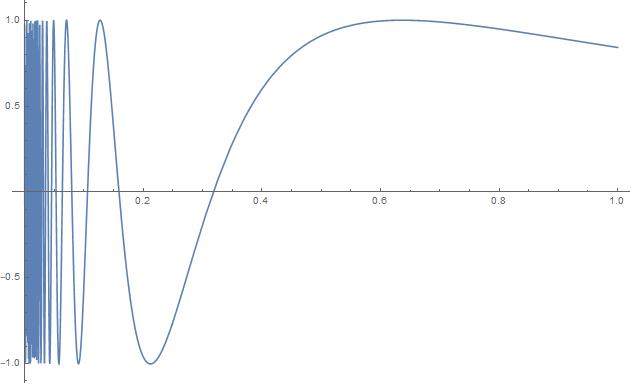
\includegraphics[scale=0.3]{figures/Top_sin.jpg}
    \caption{The topologists' sine curve}
    \label{tsine}
\end{figure}
The set is connected, since every point on the y-axis is a limit point of the curve. However, there is no continuous path connecting the y-axis to the rest of the curve, because $\sin(1/x)$ itself is not continuous.

\begin{xca}
\begin{enumerate}
    \item Show that the $n$-dimensional sphere $\bbS^n$ (defined as the unit sphere in $\bbR^{n+1}$ with the subset topology) is path-connected.
    \item Show that $\mathbb{Q}\subset\bbR $ is not connected.
    \item Show that the product of two path-connected spaces is path-connected.
\end{enumerate}
\end{xca}





\subsection{Compactness}

\begin{defn}[Covering/cover]
A collection of subsets of a topological space $X$ is said to cover $X$ if the union of these subsets equals $X$. If the subsets are all open (or closed), the covering (also often called a cover) is said to be open (resp.~closed).
\end{defn}

\begin{defn}[Compact Space]\index{Compact space}
A space $X$ is called compact if every open covering of $X$ contains a finite subcollection that also covers $X$ (\emph{subcovering}).
\end{defn}

\begin{defn}[Compact Subset]
A subset $A\subset X$ is called compact if it is compact in the subspace topology.
\end{defn}

\begin{prop}
If $Y_i\subset X$, $i = 1,\dots, m$ are compact subsets, then their union $\bigcup_{i=1}^m Y_i$ is also compact.
\end{prop}
\begin{proof}
Exercise.
\end{proof}

\begin{prop}[Compactness is a topological invariant]\label{prop f(compact)=compact}
The image $f(X)$ of a compact space $X$ under a continuous map $f\in C(X,Y)$ is compact.
\end{prop}
\begin{proof}
Exercise.
\end{proof}

\begin{xca}
\begin{enumerate}
    \item Show that the product of two connected spaces is connected. \emph{Hint:} first show that the union of any number of pairwise overlapping connected subspaces (i.e., subsets endowed with the subspace topology) of a space is also connected; then, write $X\times Y$ as the union of ``crosses'' $(\{x\}\times Y)\cup (X\times \{y\})$ that pairwise overlap and are connected only if $X$ and $Y$ are.
    \item Show that the product of two path-connected spaces is path-connected.
    \item Show that the product of two compact spaces is compact. \emph{Hint:} \cite{compact.proof}.
\end{enumerate}
\end{xca}


\begin{defn}[Classes of continuous maps]\index{Open map}\index{Closed map}\index{Proper map}
A map $f:X\to Y$ (not necessarily continuous) is called
\begin{enumerate}
    \item \emph{open} if the image of every open subset of $X$ is open in $Y$;
    \item \emph{closed} if the image of every closed subset of $X$ is closed in $Y$;
    \item \emph{proper} if it is continuous and the preimage of any compact subset of $Y$ is compact in $X$;
\end{enumerate}
\end{defn}

\begin{xca}
   Show that the image of any proper map $f:\bbR^m\to\bbR^n$ is closed.
\end{xca}






\section{Metric spaces}

\begin{defn}[Metric spaces]\index{Metric space}\index{Metric}
    A \emph{metric space} is a set $X$ with a \emph{metric} $\rho:X\times X\rightarrow \bbR $ that obeys the following conditions for any $x,y,z\in X$
\begin{enumerate}
    \item \emph{Non-negativity}: $\rho(x,y)\ge 0$; \emph{non-degeneracy:} $\rho(x,y)=0$ iff $x=y$.
    \item \emph{Symmetry}: $\rho(x,y) = \rho(y,x)$.
    \item \emph{Triangle Inequality}: $\rho(x,y) + \rho(y,z) \ge \rho(x,z)$.
\end{enumerate}
\end{defn}

\begin{defn}[Metric maps]
    A \emph{metric map} between two metric spaces $(X,\rho_X)$ and $(Y,\rho_Y)$ is a continuous map $f\in C(X,Y)$ such that $\rho_Y (f(x_1),f(x_2))\leq \rho_X (x_1,x_2)$. The category $\mathsf{Met}$ is defined as the category of metric spaces with metric maps for morphisms.
\end{defn}

\begin{defn}[Open Ball]
    An \emph{open ball} $B_r(x)$ of radius $r$ around a point $x$ in a metric space $(X,\rho)$ is defined as
\begin{equation}
    B_r(x) = \{ y\in X ~|~ \rho(y,x)< r \}
\end{equation}
\end{defn}

\begin{defn}[Metric topology]
    The metric topology induced by a metric on a set is the topology generated by basis elements that are open balls $B_r(x)$ for all $x\in X$ and $r>0$. 
\end{defn}
\begin{rem}
    Equivalently, by Proposition~\ref{characterization of topology using basis}, a set $M$ is open in the metric topology iff for any $x\in M$ there exists a radius $r>0$ such that $B_r(x)\subset M$. In the metric topology, $\rho:X\times X\to \mathbb R$ is automatically continuous.
\end{rem}
\begin{prop}
    If a metric space $(X,\rho)$ is separable, it has a countable base.
\end{prop}
\begin{proof}
    Exercise. \emph{Hint}: consider balls of rational radii about every point of the dense subset.
\end{proof}

\begin{defn}[Limit of a Sequence]
    A sequence of points $\{x_n\}$ in a metric space $X$ is said to \emph{converge} if there exists a point $x\in X$ such that for any $\epsilon >0$, there exists an $N\in \mathbb{N}$ such that
    \begin{equation}
        \forall ~ n>N,\; \rho(x_n,x) < \epsilon.
    \end{equation}
    The point $x$ is called the limit of the sequence.
\end{defn}
Note that the limit of a sequence is unique by the first axiom of the metric. One can also define the limit point of a subset of a general topological space as follows:
\begin{defn}[Limit Point]
    If $A$ is a subset of a topological space, a point $x\in X$ is said to be a limit point of $A$ if every open neighborhood of $x$ intersects $A$ in some point other than $x$.
\end{defn}

In metric spaces, limit points are equivalent to limits of sequences, i.e., for every limit point $x$ of a subset $A$, there exists a sequence of points in $A$ that converges to $x$. Conversely, for any convergent sequence of points in $A$, the limit of the sequence is a limit point of $A$.

\begin{prop}
    For a metric space $X$ equipped with the metric topology, the closure $\xoverline{A}$ of a subset $A\subset X$ is equal to the set of limit points of $A$.
\end{prop}
\begin{proof}
    Exercise.
\end{proof}

The following proposition proves the equivalence of the usual ``epsilon-delta definition'' of continuity and the topological one.

\begin{prop}
    For two metric spaces $(X,\rho)$ and $(Y,\rho')$ and a map $f:X\rightarrow Y$ such that $f(x)=y$, the following are equivalent
\begin{enumerate}
    \item $f$ is continuous at $x$.
    \item For any convergent sequence $x_n\rightarrow x$, the image is also convergent with $f(x_n)\rightarrow y$.
    \item For every $\epsilon>0$, there exists $\delta>0$ such that $\rho(x,z)<\delta \implies \rho'(f(x)=y, f(z))<\epsilon$.
\end{enumerate}
\end{prop}
\begin{proof}
    Exercise.
\end{proof}

\begin{defn}[Isometry]\index{Isometry}
    An isometry between two metric spaces is a bijective map $f:X\rightarrow Y$ that preserves distances, i.e.,
\begin{equation}
    \rho_X(x,y) = \rho_Y(f(x), f(y)).
\end{equation}
\end{defn}

\begin{prop}
    If $f:X\rightarrow Y$ is an isometry, it is also a homeomorphism.
\end{prop}
\begin{proof}
    Exercise.
\end{proof}

\begin{defn}[Equivalent metrics]\index{Metric!equivalence of}
    Two metrics $\rho_1,\rho_2$ on a topological space $X$ are called equivalent if for any $x\in X$ and any $r>0$, there exist radii $r',r''>0$ such that $B^{(1)}_{r'}(x)\subset B^{(2)}_{r}(x)$ and $B^{(2)}_{r''}(x)\subset B^{(1)}_{r}(x)$ (here, $B^{(i)}$ denotes an open ball defined by the metric $\rho_i$).
\end{defn}

\begin{thm}
    Two metrics on the same space are equivalent iff they induce the same topology.
\end{thm}
\begin{proof}
    Exercise.
\end{proof}

\begin{defn}[Cauchy sequence]\index{Cauchy sequence}
A sequence $(x_n)$ of points of a metric space $(X,\rho)$ is called a Cauchy sequence if for any $\epsilon>0$ there exists $N\in\mathbb{N}$ such that $\forall n,m\geq N$, $\rho(x_n,x_m)<\epsilon$.
\end{defn}

\begin{prop}
    A metric space is compact iff every sequence in it has a convergent subsequence (i.e.~it is \emph{sequentially compact}).
\end{prop}

\begin{defn}[Completeness]\index{Complete metric space}
A metric space $(X,\rho)$ is called complete if every Cauchy sequence $(x_n)$ in it has a limit $x_\infty\in X$.
\end{defn}


\begin{thm}[Cantor's intersection theorem]\index{Theorem!Cantor's intersection}
Let $(X,\rho)$ be a complete metric space and let $C_n$ be a sequence of closed nested subsets $C_{n+1}\subset C_n$ whose diameters tend to zero, $\mathrm{diam}\,C_n=\sup_{x,y\in C_n} \rho(x,y) \to 0$. Then the intersection $\bigcap_{n=1}^\infty C_n$ consists of exactly one point.
\end{thm}


\begin{prop}
    A metric space is sequentially compact iff every decreasing sequence of closed nonempty subsets (not necessarily tending to zero diameter) has a nonempty intersection.
\end{prop}


\begin{thm}
    A metric space is compact iff it is complete and for every $\epsilon>0$ it can be covered by a finite number of open balls of radius $\epsilon$ (i.e.~it is \emph{totally bounded}).
\end{thm}


\begin{xca}
    Consider $\mathbb{N}$ with the metric $\rho (n,m)=\lvert \frac 1 n-\frac 1 m\rvert$. Construct a sequence of balls $B_{r_k}(x_k)$ in this space such that $r_{k+1}<r_k$, $B_{r_{k+1}}(x_{k+1})\subset B_{r_k}(x_k)$, but the intersection of all these balls is empty.
\end{xca}
\begin{defn}[Normed vector space]\index{Normed vector space}\index{Norm}
    A normed vector space is a vector space $V$ over a subfield of $\mathbb{C}$ with a function (called the norm) $\lVert \cdot \rVert: V\to \mathbb{R}_+$ such that for all $x,y\in V$:
    \begin{enumerate}
        \item $\lVert x\rVert\geq 0$, and $\lVert x\rVert= 0$ iff $x=0$;
        \item $\lVert \alpha  x\rVert=\lvert \alpha \rvert \lVert x\rVert$ for any scalar (element of the structure field) $\alpha$;
        \item $\lVert x+y\rVert\leq \lVert x\rVert+\lVert y\rVert$.
    \end{enumerate}
    Every normed vector space has a naturally induced metric $\rho (x,y)=\lVert x-y\rVert$. In the corresponding induced topology, the norm is automatically continuous.
\end{defn}
\begin{defn}[Equivalent norms]\index{Norm!equivalence of}
    Two norms $\lVert\cdot \rVert_1,\lVert\cdot \rVert_2 $ on a vector space $X$ are called equivalent if there are (universal) constants $\alpha,\beta >0$ such that for all $x\in X$ we have $\alpha \lVert x \rVert_1\leq \lVert x \rVert_2 \leq \beta \lVert x \rVert_1$.
\end{defn}
Notice how this condition is much stronger than just the equivalence of the induced metrics, since $\alpha$ and $\beta$ are required to be universal constants for all $x$.

\begin{thm}
    Two norms on a vector space $X$ are equivalent iff they induce the same topology.
\end{thm}
\begin{proof}
    Exercise.
\end{proof}






\section{Separation axioms} \label{Separation Axioms}

We saw that every metric space has a canonical topology associated with it. A natural question to ask is whether the converse is true. Given a topological space, when can we define a metric on it such that the topology coincides with the metric topology? Clearly, a metric space has more structure than a topological space. In order to add more structure to topological spaces, we define the following axioms

\begin{defn}[Separation Axioms]\index{Separation axioms}
    For a topological space $X$ with arbitrary points $x$ and $y$ and arbitrary disjoint closed sets $F$ and $G$, we define the following axioms:
    \begin{enumerate}
        \item $T_0$ (\emph{Kolmogorov}): There exists an open neighborhood $U$ of $x$ that doesn't include $y$, \emph{or} an open neighborhood $V$ of $y$ that doesn't include $x$. \index{Kolmogorov space}
        \item $T_1$: There exists an open neighborhood $U$ of $x$ that doesn't include $y$, \emph{and} an open neighborhood $V$ of $y$ that doesn't include $x$, i.e., $x$ and $y$ are \emph{separated}.
        \item $T_2$ (\emph{Hausdorff}): There exist disjoint open neighborhoods $U$ of $x$ and $V$ of $y$, i.e., $x$ and $y$ are \emph{separated by neighborhoods}.\index{Hausdorff space}
        \item $T_3$: There exist disjoint open neighborhoods $U$ of $x$ and $V$ of $F$.
        \item \emph{Regular}: $X$ is both $T_1$ and $T_3$.
        \item $T_4$: There exist disjoint open neighborhoods $U$ of $F$ and $V$ of $G$.
        \item \emph{Normal}: $X$ is both $T_1$ and $T_4$.
    \end{enumerate}
\end{defn}

\begin{figure}[tp]
    \centering
    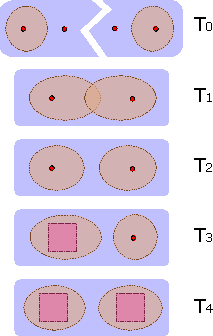
\includegraphics[scale=1.0]{figures/separation-axioms.pdf}
    \caption{Separation axioms. Red dots are points, ovals are open sets and squares are closed sets. [\href{http://mathroughguides.wikidot.com/article:point-set-topology}{Source}]}
\end{figure}

\begin{prop}
    The following results demonstrate how each axiom adds additional structure to the space:
\begin{enumerate}
    \item $T_1 \implies$ All finite sets are closed;
    \item $T_2\implies T_1$;
    \item Regular $\implies$ Hausdorff;
    \item Normal $\implies$ Regular.
\end{enumerate}
\end{prop}

\begin{example}
    The category $\mathsf{Hausd}$ of Hausdorff spaces is a full subcategory of $\mathsf{Top}$.
\end{example}

\begin{thm}[Urysohn Lemma]\index{Lemma!Urysohn}
    A space $X$ is normal iff for any two disjoint closed subsets $A$ and $B$ there exists a continuous function
\begin{equation}
f\in C(X,[0,1]) ~\text{such that}~ \restr{f}{A} = 0, \restr{f}{B} = 1.
\end{equation}
\end{thm}

\begin{thm}
    All metric spaces are normal.
\end{thm}
\begin{proof}
    Exercise.
\end{proof}

\begin{thm}[Urysohn]
    A normal space with a countable base is \emph{metrizable}, i.e., we can construct a canonical metric whose induced topology coincides with the topology of the space.
\end{thm}

\begin{prop}
    If $X$ is Hausdorff, every compact subset of $X$ is closed.
\end{prop}
\begin{proof}
    Exercise. \emph{Hint:} prove that the complement of the compact set is open by using Proposition~\ref{open iff contains neighborhoods}.
\end{proof}

\begin{prop}
    Every compact Hausdorff space is normal.
\end{prop}
\begin{proof}
    Exercise.
\end{proof}

\begin{thm}[Heyne-Borel]\index{Theorem!Heyne-Borel}
    In Euclidean space $\bbR^n$, a subset is compact iff it is closed and bounded.
\end{thm}

The following theorem is one of the most fundamental theorems in functional analysis, and it essentially characterizes compact subsets of the set of continuous functions defined on a compact subset of $\bbR^n$. We state it simply as an example of usage of the above topological terminology.
\begin{thm}[Arzel\`a-Ascoli]\index{Theorem!Arzel\`a-Ascoli}
    Let $X$ be a compact Hausdorff space. A subset $F$ of the space $C(X,\bbR )$ of continuous real-valued functions on $X$ is relatively compact (i.e., its closure is compact) in the topology given by the sup-norm $\lVert f\rVert=\sup_X \vert f\rvert$ iff it is equicontinuous (i.e., all elements $f\in F$ are uniformly continuous functions and the $\delta$ in the definition of uniform continuity is universal for all $f\in F$) and pointwise bounded (i.e., for every $x\in X$ the set $\{f(x)\}_{f\in F}$ is bounded).
\end{thm}







\section{Homotopy}\label{sec.homotopy}

\begin{defn}[Homotopic maps]\index{Homotopy} 
    Two continuous maps $f_0,f_1\in C(X, Y)$ are called homotopic (we often write $f\sim g$) if there exists a continuous map, called homotopy, $F\in C([0,1]\times X,Y)$ such that $F(0,x)=f_0(x)$ and $F(1,x)=f_1(x)$. Here, $[0,1]$ has the standard topology. For convenience, we will often describe homotopies as \emph{families of maps} $f_t:X\to Y$ defined by $f_t(x)=f(t,x)$.
\end{defn}
\begin{prop}
    Homotopy is an equivalence relation on $C(X,Y)$. (The set of all homotopy classes of continuous maps from $X$ to $Y$ is denoted by $[X,Y]$. This set defines the morphisms in the (naive) homotopy category $\mathsf{hTop}$.)
\end{prop}
\begin{proof}
    Exercise.
\end{proof}

The first argument of $F(t,x)$ is essentially ``time'', and $F(t,\cdot)$ continuously interpolates between $f_0$ and $f_1$ as time goes from 0 to 1. In topology, homotopy is synonymous with the phrase ``continuous deformation''.


\begin{defn}[Contractible space]\index{Contractible space}
    A space $X$ is called contractible if it is homotopy equivalent to the one-point space, i.e., there exists a point $x_0\in X$ such that the constant map $f(x)=x_0$ is homotopic to the identity, $f\sim \id_X$. This property is in fact independent of $x_0$.
\end{defn}
\begin{prop}
    Any contractible space is path-connected.
\end{prop}
\begin{proof}
    Exercise. \emph{Hint:} consider paths traced out by $F(t,x)$ for fixed $x$'s.
\end{proof}
\begin{example}
\begin{enumerate}
    \item $\bbR^n$, $B^n$, $(0,1)^n$ are all contractible via, say, $F(t,x)=tx$ (they are also all homeomorphic to each other).
    \item Any two continuous functions $f,g:\bbR \to\bbR $ are homotopic via homotopy $F(t,x)=tg(x)+(1-t)f(x)$.
\end{enumerate}
\end{example}
\begin{xca}
    Show that if $Y$ is contractible, then any two maps $f,g\in C(X,Y)$ are homotopic. This is a generalization of the above example for $X=Y=\bbR $.
\end{xca}
\begin{thm}[Brouwer]
    The sphere $\bbS^n$ is not contractible.
\end{thm}
\begin{proof}
    There is a plethora of different ways to prove this theorem, from pure analytical to algebraic. We will delay the proof until we compute the homology groups of the spheres in Part \ref{Part II} and observe that they differ from those of a contractible space (and homology groups are topological invariants).
\end{proof}
\begin{thm}[Brouwer's fixed point theorem]\index{Theorem!Brouwer's fixed point}\label{thm Brouwer's fixed point}
    Any continuous map $f\in C\left(\xoverline{B^n},\xoverline{B^n}\right)$  from the closed unit ball to itself has at least one fixed point ($x_0$ such that $f(x_0)=x_0$).
\end{thm}
\begin{proof}
    For $n=1$ this is clear. For $n\geq 2$, suppose $f(x)\neq x$ for all $x$. Then we can define $h(x)$ as the point of intersection of the ray $[f(x),x)$ with the boundary of the ball. Then $F(t,x)=h(tx)$ is a contracting homotopy, which contradicts the last theorem.
\end{proof}
\begin{rem}
    These two theorems are in fact equivalent. The fixed point theorem can be proven purely analytically, and the contractibility theorem will follow. The simplest modern proof of non-contractibility of $\bbS^n$ is based on homology.
\end{rem}

\begin{defn}[Retraction, Deformation retraction]\index{Retraction}\index{Deformation!retraction}
    A retraction of a topological space $X$ onto its subspace $A\subset X$ is a continuous map $r:X\to A$ such that $\restr{r}{A}=\mathrm{id}_A$. A deformation retraction is a homotopy from the identity map $\mathrm{id}_X$ to $r$. A \emph{strong} deformation retraction also satisfies $\restr{r_t}{A}=\mathrm{id}_A$ for all $t\in[0,1]$ (this is often included in the definition of a deformation retraction).
\end{defn}

\begin{defn}[Homotopy equivalence of spaces]\index{Homotopy equivalence}
    Two topological spaces $X$ and $Y$ are called homotopy equivalent if there exist two continuous maps $f\in C(X,Y)$, $g\in C(Y,X)$ such that their compositions are homotopic to identity: $g\circ f\sim \id_X$ and $f\circ g\sim \id_Y$. We write $X\simeq Y$.
    In the presence of basepoints, these homotopies are required to leave the basepoints fixed for all values of the deformation parameter $t$.
\end{defn}

\begin{cor}
    \begin{enumerate}
        \item Deformation retractions are homotopy equivalences.
        \item Contractible spaces are homotopy equivalent to a point.
    \end{enumerate}
\end{cor}

\begin{example}
\begin{enumerate}
    \item $\bbS^1\times\bbR \simeq \bbS^1\simeq M$, where $M$ is the M\"obius band.
    \item $\bbR^n\setminus{0}\simeq \bbS^{n-1}$.
    \item More generally, two spaces $X,Y$ are homotopy equivalent iff they are both deformation retracts of the same space $Z$. That is, there needs to exist $A_X\subset Z$ such that $A_x\cong X$ and there exists a continuous map $F\in C([0,1]\times Z,Z)$ such that $F_X(0,z)=z$, $F_X(1,z)\in A$ and $F_X(t,a)=a$ for any $z\in Z$, $t\in [0,1]$ and $a\in A_x$. Similarly, there needs to exist $A_Y\subset Y$ homeomorphic to $Y$ that is a deformation retract of $Z$.
\end{enumerate}
\end{example}






\section{Fundamental group}

\begin{defn}[Loops, Pointed homotopy]\index{Loop}
    Let $X$ be a path-connected topological space, pick a ``base point'' $x_0\in X$, and consider the set of all \emph{loops} in $X$ based at $x_0$, i.e., paths $\gamma\in C([0,1], X)$ such that $\gamma(0)=\gamma(1)=x_0$. A pointed homotopy between two such loops is a homotopy $F\in C([0,1]\times[0,1],X)$ such that $F(\cdot,0)=F(\cdot,1)=x_0$. Pointed homotopy is an equivalence relation on the set of based loops.
\end{defn}

\begin{defn}[Fundamental/Poincar\'e group]\index{Fundamental group}
    The fundamental group $\pi_1(X,x_0)$ of a path-connected space $X$ with a base point $x_0$ is defined as the set $\{ [\gamma]\}$ of pointed homotopy classes of based loops with the inversion operation given by $[\gamma(t)]^{-1}=[\gamma(1-t)]$ and the multiplication operation 
    \[
    [\gamma_1(t)]\circ [\gamma_2(t)]=\left[ \begin{cases} \gamma_1(2t), & t\in[0,1/2], \\ \gamma_2(2t-1), & t\in(1/2,1] \end{cases}\right].\label{pi1 group op}
    \]
    The unit element is given by the equivalence class of the ``constant loop'' $\gamma(t)\equiv x_0$. If $X$ is not path-connected, then $\pi_1(X,x_0)$ is defined as the fundamental group of the path-connected component containing $x_0$.
\end{defn}

\begin{xca}
    Check that this definition is consistent, i.e., the homotopy classes on the right-hand sides don't depend on the choices of representatives of the classes on the left.
\end{xca}
\begin{defn}[Simple-connectedness]\index{Simply connected space}
    A path-connected space $X$ is called simply connected if its fundamental group is trivial, $\pi_1(X,x_0)=\{e\}$.
\end{defn}

\begin{xca}
Show that contractible spaces are simply connected.
\end{xca}

\begin{thm}
    If a space $X$ retracts onto a subspace $A$, then the homomorphism of fundamental groups $i_\ast:\pi_1(A,x_0)\to \pi_1(X,x_0)$ induced by the inclusion $i: A\hookrightarrow X$ is injective. If $A$ is a deformation retract of $X$, then $i_\ast$ is an isomorphism.
\end{thm}
\begin{proof}
    If $r:X\to A$ is a retraction then $r\circ i=\mathrm{id}_A$, hence by functoriality of $\pi_1$, $r_\ast \circ i_\ast=\mathrm{id}_{\pi_1(A,x_0)}$, which implies injectivity. If $r_t$ is a deformation retraction, then for any loop $\gamma$ in $X$ based at $x_0\in A$ the composition $r_t\circ \gamma$ gives a homotopy of $\gamma$ to a loop in $A$, therefore $i_\ast$ is also surjective.
\end{proof}

\begin{defn}[Alternative approach]
    Recall that the category $\mathsf{Top}_\bullet$ consists of ``pointed topological spaces'' with chosen basepoints and morphisms that are continuous maps mapping basepoint to basepoint. Take the circle $\bbS^1$ and pick a point $\bullet$ in it. Then one can redefine based loops as morphisms between two pointed topological spaces $\gamma\in C((\bbS^1,\bullet),(X,x_0))$. Pointed homotopy in the definition of $\pi_1$ can then be replaced by just homotopy of loops as maps defined on $\bbS^1$.   Thus, as a set, $\pi_1(X)=[\bbS^1,X]_\bullet$ (group of homotopy classes of pointed maps).
\end{defn}

\begin{defn}[Suspension]\index{Suspension}
    The suspension of a topological space $X$, is defined as the quotient space $SX=(X\times [0,1])/(X\times \{0\},X\times\{1\})$ (i.e., a cylinder over $X$ where each of the two faces is then collapsed into a point -- best visualized as a double cone over $X$). If $X$ is a pointed space with basepoint $x_0$, then the \emph{reduced suspension} is defined as $\Sigma X=(X\times [0,1])/(X\times \{0\},X\times\{1\} ,\{x_0\}\times [0,1]))$, and the new basepoint is the image of $(x_0,0)$ in the quotient. Equivalently, $\Sigma X=X\wedge \bbS^1=X\times \bbS^1/(X\vee \bbS^1)$.
\end{defn}

\begin{xca}
    Verify that $\Sigma$ extends to a functor on the category of pointed spaces. This will follow from the uniqueness of the pointed map at the bottom of the following square that makes it commute:
    \[\begin{tikzcd}[every matrix/.append style={name=m},   
    execute at end picture={\draw [<-] ([xshift=-2.3em,yshift=1mm]m-2-2.north) arc[start angle=-90,delta angle=270,radius=0.25cm];}]
   X \arrow[r,"f"]\arrow[d,swap,"\pi_X"]& Y\arrow[d,"\pi_Y"] \\
   \Sigma X\arrow[r,swap,dashed, "\exists !\,\Sigma(f)"]& \Sigma Y
    \end{tikzcd}\]
    where $\pi_X$ and $\pi_Y$ are the quotient maps that define the suspensions.
\end{xca}

\begin{example}
    From Exercise~\ref{wedge sums} we have $\Sigma \bbS^n\cong \bbS^{n+1}$. This holds even when $n=0$ and $\bbS^0=\{-1,1\}$.
\end{example}

\begin{defn}[Compact-open topology]
    Given two spaces $X,Y$, denote the set of all continuous maps between them by $Y^X=C(X,Y)$. The compact-open topology on $Y^X$ is generated\footnote{The topology generated by a collection of sets is simply the coarsest topology in which all of those sets are open. This topology consists of all unions and all finite intersections of these sets.} by the sets $M(K,U)=\{f\in Y^X\mid f(K)\subset U\}$ where $K\subset X$ is compact and $U\subset Y$ is open.
\end{defn}

\begin{prop}
    If $X,Y$ are Hausdorff and $X$ is locally compact, then $C(X,Y)$ is Hausdorff.
\end{prop}
\begin{proof}
    Let $f,g\in C(X,Y)$ with an $x\in X$ such that $f(x)\neq g(x)$. Since $Y$ is Hausdorff, there exist disjoint open neighborhoods $U_1$ of $f(x)$ and $U_2$ of $g(x)$. Then $f^{-1}(U_1)\cap g^{-1}(U_2)$ is an open neighborhood of $x$, because $f$ and $g$ are continuous. Since $X$ is locally compact, this neighborhood contains a compact neighborhood $K$. Then, $M(K,U_1)$ and $M(K,U_2)$ are neighborhoods of $f$ and $g$, respectively. They are disjoint because $U_1$ and $U_2$ are.
\end{proof}

\begin{prop}
    If $X$ is a locally compact Hausdorff space, then the evaluation map $e:Y^X\times X\to Y$, defined by $e(f,x)=f(x)$, is continuous.
\end{prop}
\begin{proof}
    Let $U$ be an open neighborhood of $f(x)$. Since $f$ is continuous and due to the properties of $X$, there is a compact neighborhood $K$ of $x$ such that $f(K)\subset U$. Thus $f\in M(K,U)$ and $M(K,U)\times K$ is mapped into $U$ by the evaluation map $e$. Finally, $M(K,U)\times K \subset Y^X\times X$ is a neighborhood of $(f,x)$. This proves continuity.
\end{proof}


\begin{thm}[{{\cite[Thm.~VII.2.4]{Bredon}}}]\label{compact open continuity}
    Let $X$ be a locally compact Hausdorff space, and $Y$ and $T$ Hausdorff spaces. For any map $f:X\times T\to Y$, denote $f_t(x)=f(x,t)$. Then the continuity of $f$ is equivalent to each $f_t$ being continuous separately and the mapping $t\mapsto f_t$ also being continuous from $T$ into $Y^X$. 
\end{thm}

This theorem implies that if $X$ is locally compact, then a homotopy $X\times [0,1]\to Y$ is the same thing as a path $[0,1]\to Y^X$.
\begin{cor}[The Exponential Law {{\cite[Thm.~VII.2.5]{Bredon}}}]
    Let $X,T$ be locally compact Hausdorff spaces, and $Y$ a Hausdorff space. Then the bijection from Theorem~\ref{compact open continuity} is a natural homeomorphism $Y^{X\times T}\cong \left(Y^X\right)^T$ taking $f$ to $f^\ast$ defined as $f^\ast (t)(x)=f(x,t)=f_t(x)$.
\end{cor}

Similarly, one can show that under similar conditions, one has homeomorphisms $Y^X\times W^X\cong (Y\times W)^X$ (under $f\times g$), $Y^{X\sqcup T}\cong Y^X\times Y^T$ (under $f\sqcup g$), and $Z^Y\times Y^X \cong Z^X$ (under $f\circ g$). For details see \cite[\S VII.2]{Bredon}.
\begin{defn}[Loop space]\index{Loop space}
    The loop space of a pointed space $X$ is the space $\Omega X=X^{\bbS^1}$ that consists of loops based at $x_0$, with the compact-open topology. Its basepoint is the constant loop at $x_0$.
\end{defn}


\begin{prop}\label{suspension maps prop}
    \begin{enumerate}
        \item The set of homotopy classes $[X;\Omega Y]$ is a group under the multiplication induced by the usual multiplication of loops in $Y$;
        \item The set of homotopy classes $[\Sigma X;Y]$ is a group under the multiplication induced by the concatenation of maps along the interval $[0,1]\times\{x_0\}$ in $\Sigma X$ (namely $f(2t,x)$ for $t\leq 1/2$ and $g(2t-1,x)$ after that);
        \item On the set $[\Sigma X;\Omega Y]$, the two multiplications defined above coincide and are abelian.
    \end{enumerate}
\end{prop}
\begin{proof}
    Item 1 is obvious and Item 2 is easily checked by verifying that the concatenation of a map with its time-reversed copy, $f(1-t,x)$, is homotopic to the constant map.

    In item 3, such maps can be denoted $f_{t,s}(x)$, where $t$ is the parameter in $\Sigma X$ and $s$ is the one in $\Omega Y$. The two multiplications differ only in which of these two parameters maps get concatenated along. The idea is then to homotopically deform one into the other. This can be done by using a deformation retract of the square $[0,1]^2$ into a smaller square in the center.  Since we're working with pointed spaces, the whole boundary of the square gets mapped to the basepoint $y_0$. Hence we can replace $f$ and $g$ with their retractions to the smaller square, whereas outside of that square the value is just $y_0$. Now the two different concatenations are clearly homotopic to each other since we can smoothly ``slide'' the domains of $f$ and $g$ around each other, and then undo the original deformation retract. This proves both the equality of the two products and their commutativity. See figure.
    \begin{center}
    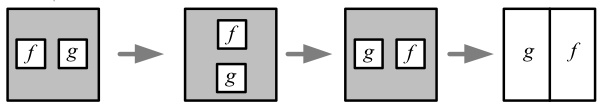
\includegraphics[scale=1]{figures/higher-homotopy.png}
    \end{center}
\end{proof}

\begin{lem}\label{lemma on suspension and loops}
    For any pair of pointed spaces $X,Y$, there is a natural isomorphism of groups $[\Sigma X,Y]\approx [X,\Omega Y]$.
\end{lem}
\begin{proof}
    The isomorphism is induced by the correspondence that identifies $f(t,x)$ with $\gamma(x)(t)=f(t,x)$. One can easily check that this provides a one-to-one correspondence between pointed maps and pointed homotopy on both sides. Furthermore, it is almost obvious that the multiplication on both sides works the same way.
\end{proof}

\begin{defn}[Zeroth degree homotopy set]
    Denote by $\pi_0(X)$ the set of path-connected components of $X$. It can be identified with the set of homotopy equivalence classes of maps from the one-point space into $X$. Note that this set carries no natural structure of a group.
\end{defn}

\begin{rem}
    One of the most useful consequences of the above discussion is that in sufficiently nice topological categories, such as that of topological manifolds, homotopies are just paths in the space of continuous maps. Therefore homotopy classes of maps $[X;Y]$ are nothing but the path-connected components in the space $Y^X$, that is, $\pi_0( Y^X)$. For compact $X$ Lemma~\ref{lemma on suspension and loops} can be shown indirectly using the exponential law, $Y^{\Sigma X}\cong (\Omega Y)^X$. As we've just seen, the multiplications on these spaces correspond, thus we have group homomorphisms $[\Sigma X;Y]= \pi_0(Y^{\Sigma X})\cong \pi_0((\Omega Y)^X)= [X;\Omega Y]$.
\end{rem}
\begin{prop}\label{prop computing pi1}
\begin{enumerate}
    \item $\pi_1$ is a covariant functor $\pi_1:\mathsf{Top}_\bullet\to \mathsf{Gr}$.
    \item For a path-connected space, fundamental groups with different base points are isomorphic (this is why we often abuse the notation by writing $\pi_1(X)$).
    \item For any number of path-connected spaces, $\pi_n(\prod_\alpha X_\alpha)\cong \prod_\alpha \pi_n(X_\alpha)$.
\end{enumerate}
\end{prop}
\begin{proof}
Exercise.
\end{proof}

\begin{lem}\label{lem product of loops}
    If a space $X$ is the union of a collection of path-connected open sets $U_\alpha$ each containing the basepoint $x_0$ and if each intersection $U_{\alpha\beta}$ is path-connected, then every loop in $X$ at $x_0$ is homotopic to a product of loops each of which is contained in a single $U_\alpha$.
\end{lem}
\begin{proof}
    The key is in the compactness of the interval $[0,1]$, which guarantees that the loop can be broken up into a finite number segments each of whose closure is contained inside only one of the $U_\alpha$'s. Call these segments $f_i, i=1,\ldots,n$. Since $x_0$ belongs to each $U_\alpha$, we can then find a path $g_i$ from $x_0$ to the starting point of $f_i$. We can always choose $g_0$ and $g_{n+1}$ to be trivial. The loops we seek are then $g_i\cdot f_i\cdot g_{i+1}^{-1}$. Their product is homotopic to the original loop because all $g_i$'s cancel out.
\end{proof}
\begin{cor}\label{cor pi_1(S^n)=0}
    $\pi_1(\bbS^n)=0$ for $n\geq 2$.
\end{cor}
\begin{proof}
    $\bbS^n$ is the union of the open neighborhoods of two hemispheres, $U_+$ and $U_-$. Each of these is homeomorphic to $\bbR^n$ and $U_+\cap U_-\cong \bbS^{n-1}\times \bbR $. If $n\geq 2$, then $U_+\cap U_-$ is path-connected. By the above lemma, every loop in $\bbS^n$ based at a point $x_0\in U_+\cap U_-$ is a product of two loops within each hemisphere. However both of these loops are trivial since $\pi_1(U_\pm)=0$.
\end{proof}
\begin{cor}
    $\bbR^2$ is not homeomorphic to $\bbR^n$ for $n\neq 2$.
\end{cor}
\begin{proof}
    Assume there is a homeomorphism $f:\bbR^2\to \bbR^n$. The case $n=1$ is easy because $\bbR \setminus\{f(0)\}$ is not connected whereas the supposedly homeomorphic $\bbR^2\setminus\{0\}$ is. 
    When $n>2$, the complement $\bbR^n\setminus\{f(x)\}$ is homeomorphic to $\bbS^{n-1}\times \bbR $, whose fundamental group is $\pi_1(\bbS^{n-1})=0$ by Proposition~\ref{prop computing pi1}. However, for $n>2$ the fundamental group of the complement $\bbR^2\setminus\{x\}$ is $\pi_1(\bbS^1)=\bbZ$. This leads to a contradiction.
\end{proof}

We are now prepared to prove one of the most important theorems about the fundamental group. First let us recall the categorical notion of pushouts (see Definition~\ref{pushouts}). If a path-connected space is represented as a union of two open sets, $X=U\cup V$, then the corresponding set inclusions induce homomorphisms of fundamental groups:
\[
    \begin{tikzcd}[every matrix/.append style={name=m},   
    execute at end picture={\draw [<-] ([xshift=-8.5mm,yshift=1mm]m-2-2.north) arc[start angle=-90,delta angle=270,radius=0.25cm];}]
    X \arrow[r,leftarrow,"l"]\arrow[d,leftarrow,"k"]& V\arrow[d,leftarrow,"j"] \\
    U\arrow[r,,leftarrow,swap,"i"]& U\cap V\\
    \end{tikzcd}
    \quad\quad\quad\quad\quad
    \begin{tikzcd}[every matrix/.append style={name=m},   
    execute at end picture={\draw [<-] ([xshift=-11.5mm,yshift=1mm]m-2-2.north) arc[start angle=-90,delta angle=270,radius=0.25cm];}]
    \pi_1(X) \arrow[r,leftarrow,"l_\ast"]\arrow[d,leftarrow,"k_\ast"]& \pi_1(V)\arrow[d,leftarrow,"j_\ast"] \\
    \pi_1(U)\arrow[r,,leftarrow,swap,"i_\ast"]& \pi_1(U\cap V)\\
    \end{tikzcd}
\]
$X$ itself is in fact the pushout, $X=U\sqcup_{U\cap V}V$. \emph{The Siefert-van~Kampen theorem will show that the functor $\pi_1$ preserves pushouts,} i.e., the fundamental group of the union is isomorphic to the amalgamated free product, $\pi_1(X)\cong \pi_1(U) \ast_{\pi_1(U\cap V)} \pi_1(V)$. By the universal property of the free product, there is a unique homomorphism $\Phi$ in the diagram below that makes the external triangles commute.
\[
    \begin{tikzcd}
    \pi_1(U)\ast \pi_1(V)   \arrow[drr,leftarrow, bend left]   \arrow[ddr,leftarrow, bend right]   \arrow[dr,"\exists! \Phi" description] & & \\
        & \pi_1(X) \arrow[r,leftarrow,swap, "l_\ast"] \arrow[d,leftarrow, "k_\ast"]       & \pi_1(V) \arrow[d,leftarrow, "j_\ast"] \\ & \pi_1(U) \arrow[r,leftarrow,swap, "i_\ast"] &\pi_1(U\cap V) 
    \end{tikzcd}
\]
Note, however, that the ``background square'' involving $\pi_1(U\cap V),\pi_1(U),\pi_1(V)$, and $\pi_1(U)\ast \pi_1(V)$ \emph{does not commute}, so the universal property of the pushout \emph{will not} apply in the other direction to give a homomorphism $\pi_1(X)\to \pi_1(U)\ast\pi_1(V)$. Instead, we will compute $\pi_1(X)$ by finding the kernel of $\Phi$ and factoring it out.

\begin{thm}[Siefert-van Kampen {{\cite[Thm.~1.20]{Hatcher}}}]\index{Theorem!Siefert-van~Kampen}\label{thm seifert-van kampen}
    If $X$ is the union of path-connected open sets $U_\alpha$ each containing the basepoint $x_0\in X$ and if each intersection $U_{\alpha\beta}$ is path-connected, then the homomorphism $\Phi: \ast_\alpha \pi_1(U_\alpha)\to \pi_1(X)$ induced by the inclusions $U_\alpha \hookrightarrow X$ is surjective. 
    
    Denote the inclusion-induced homomorphisms $i_\alpha:\pi_1(U_\alpha)\to \pi_1(X)$ and $i_{\alpha\beta}:\pi_1(U_{\alpha\beta})\to \pi_1(U_\alpha)$. We have $i_\alpha \circ i_{\alpha\beta}=i_{\beta}\circ i_{\beta\alpha}$ since both sides are induced by the inclusion $U_{\alpha\beta}\hookrightarrow X$. Now, if in addition each intersection $U_{\alpha\beta\gamma}$ is path-connected, then the kernel of $\Phi$ is the normal subgroup $N$ generated by all elements of the form $i_{\alpha\beta }(g)i_{\beta\alpha}(g)^{-1}$ for $g\in\pi_1(U_{\alpha\beta})$, and hence $\Phi$ induces a homomorphism $\pi_1(X)\cong \ast_\alpha \pi_1(U_\alpha)/N$.

    In particular, in the case of two sets, $\pi_1(U\cup V)\cong \pi_1(U)\ast_{\pi_1(U\cap V)}\pi_1(V)$.
\end{thm}
\begin{proof}
    The surjectivity of $\Phi$ was already shown in Lemma~\ref{lem product of loops}. 
    
    Now we need to show that the kernel of $\Phi$ is exactly $N$. We already know that $N\subset \ker \Phi$ since $i_\alpha\circ i_{\alpha\beta}=i_\beta\circ i_{\beta\alpha}$. For the reverse inclusion, the idea is to study \emph{factorizations} of loops into ``smaller'' loops $[\gamma_i]$ that are completely contained in one of the $U_\alpha$'s. There are two ``moves'' that, as we would like to show, transform differing factorizations of the same loop into each other. Namely, a substring of the form $[\gamma_i][\gamma_{i+1}]$ can be replaced with $[\gamma_i\cdot \gamma_{i+1}]$, and an element $[\gamma_i]$ viewed as an element of $\pi_1(U_\alpha)$ can be replaced with its analog in $\pi_1(U_\beta)$ if $\gamma_i$ is a loop contained in $U_{\alpha\beta}$. If we can show that all factorizations of a loop can be transformed into each other via a sequence of moves of this kind (or their inverses), that will mean that $\Phi$ induces an \emph{injective} map from the quotient group into $\pi_1(X)$, and thus the kernel of $\Phi$ is exactly $N$.

    The goal is therefore to decompose any homotopy of loops into a sequence of moves like this. A homotopy is a continuous map defined on the unit square, $H:[0,1]\times[0,1]\to X$, whose value on the left and right edges of the square is $x_0$. Now we need to subdivide this square into smaller squares as in the Figure, so that each square is mapped entirely into only one of the open sets $U_\alpha$, and so that the resulting subdivisions of the top and bottom edges of the square are refinements of the subdivisions implied in the two factorizations at hand (that is, each interval of the new subdivision is entirely contained in an interval from the old). Lastly, we can ``perturb'' the squares in the central rows so that each point is contained in at most three squares (this is why triple intersections were required to be path-connected).

    \begin{center}
        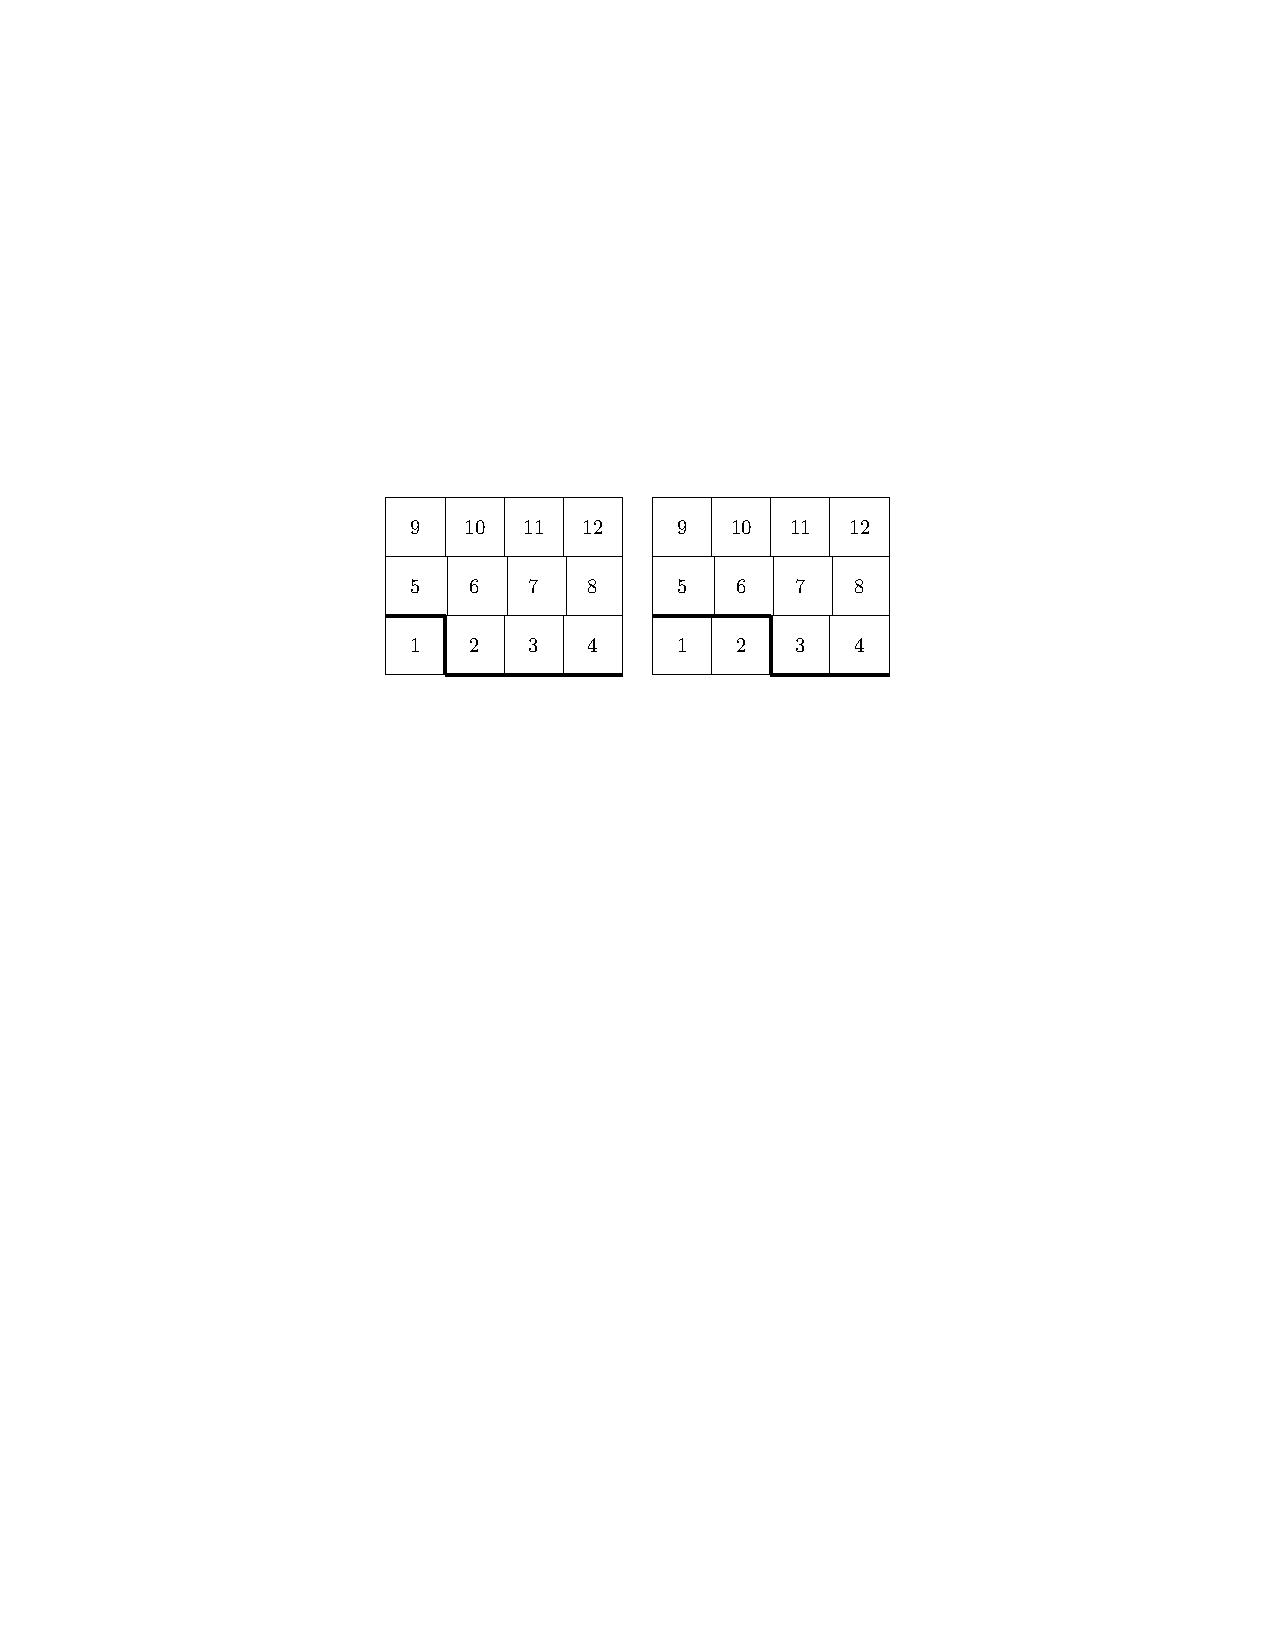
\includegraphics[scale=0.75]{figures/subdivision.pdf}
    \end{center}

    Now we proceed to define a sequence of paths along the edges of the subdivision from the left to the right side of the square that progressively ``capture'' more and more of the squares. For each segment we need to specify which of the open sets in $X$ its image is supposed to belong to, which is exactly the second move (in other words, $i_{\alpha\beta\ast}([\gamma_i])$ and $i_{\beta\alpha\ast}([\gamma_i])$ belong to the same coset in the quotient group). Further, each successive path is homotopic to the last via a deformation of a loop inside one $U_\alpha$. All together, this proves that any two factorizations of the same loop are equivalent in the sense that they differ only by relations that define the group $N$. The illustration below is from \cite[Chapter 10]{LeeTop}.

    \begin{center}
        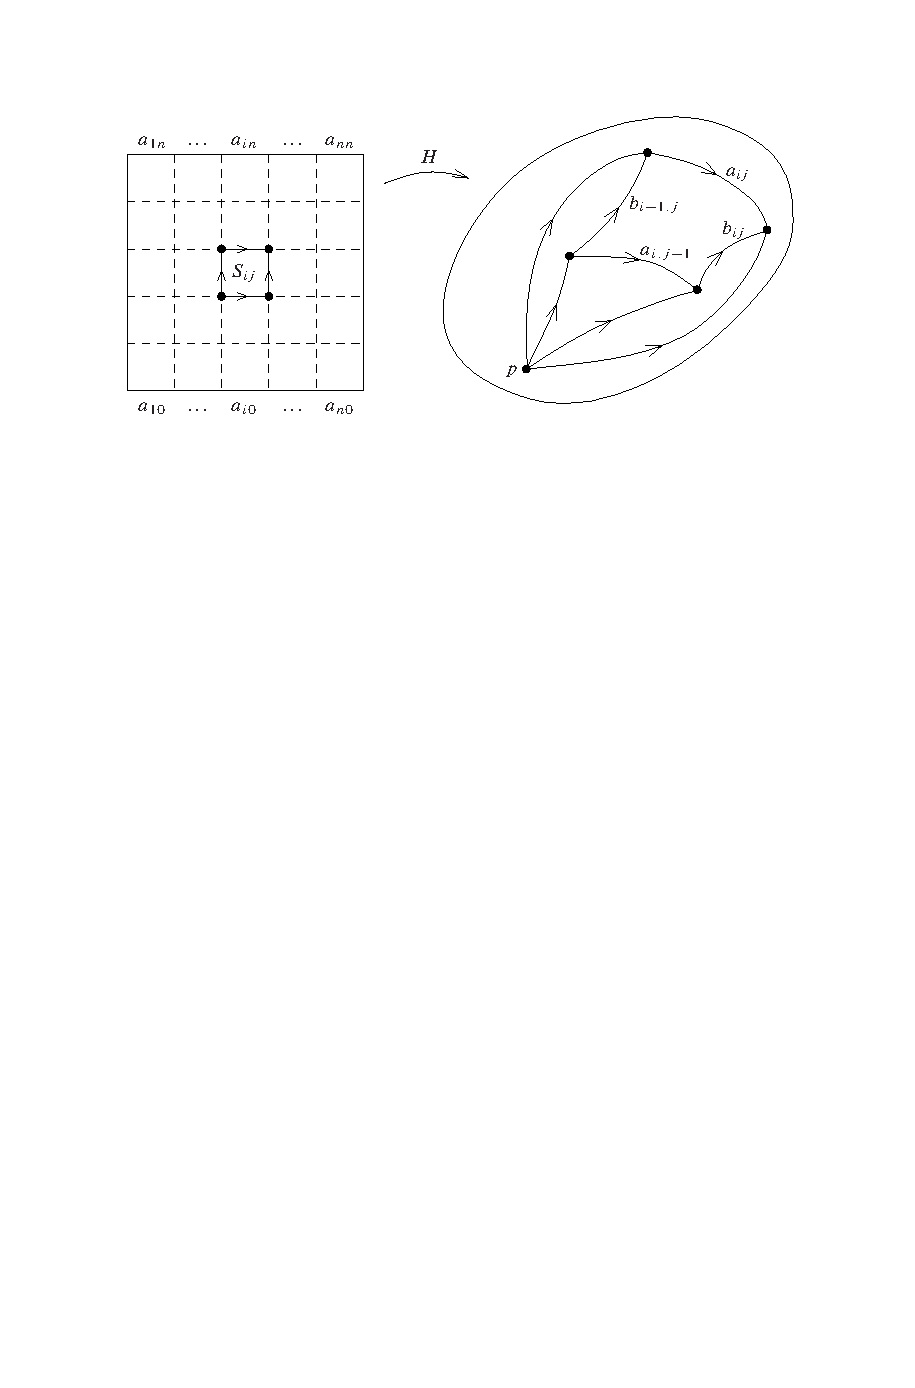
\includegraphics[scale=1]{figures/kernel of Phi.pdf}
    \end{center}
    
    See \cite[Thm.~1.20]{Hatcher} for more details of the proof.
\end{proof}

The conditions on path-connectedness of intersections and on the basepoint seem artificial, and indeed the are. Any open covering of $X$ can be turned into a cover of this kind by taking unions of sets lying along paths connecting them to the original basepoint. The full version of the Seifert-van~Kampen theorem can be stated purely in categorical terms with no extra conditions, however first we will need the notion of the \emph{fundamental groupoid}.

\begin{defn}[Groupoid]\index{Groupoid}
    A groupoid is a set with a unary ``inversion'' map $x\mapsto x^{-1}$ and a partial (i.e., not necessarily defined for any pair of elements) associative binary ``multiplication'' operation $(x,y)\mapsto x\bullet y$. It is associative in the sense that if both $x\bullet y$ and $y\bullet z$ exist, then both $(x\bullet y)\bullet z$ and $x\bullet (y\bullet z)$ exist and coincide. It is also required that $x\bullet x^{-1}$ and $x^{-1}\bullet x$ exist, and that, if $x\bullet y$ exists, then $x\bullet y\bullet y^{-1}=x$ and $x^{-1}\bullet x\bullet y=y$.

   As a consequence of these axioms, $(x^{-1})^{-1}=x$ and $(x\bullet y)^{-1}=y^{-1}\bullet x^{-1}$. Intuitively, groupoids can be thought of as groups with many identities, where only elements belonging to the same identity (which is the case if $x\bullet x^{-1}=x\bullet x^{-1}$) can be multiplied. 
    
    An equivalent definition is that a groupoid is a category where all morphisms are invertible (i.e., isomorphisms). The objects of this category are the ``identities'' of the groupoid. A group is then simply a groupoid with a single object. The category of groupoids is denoted $\mathsf{Grpd}$.
\end{defn}

Free products of groupoids can be constructed in the same way as for groups -- as strings of ``words'' $g_1^{\epsilon_1} \cdots g_n^{\epsilon_n}$ where each product $g_i^{\epsilon_i}\bullet g_{i+1}^{\epsilon_{i+1}}$ must exist and insertions of substrings of the form $gg^{-1}$ produce an equivalent string. These free products have the same universal property and are therefore the pushouts in $\mathsf{Grpd}$.

\begin{defn}[Fundamental groupoid]\index{Fundamental groupoid}
    Given a topological space $X$, let $\Pi(X)$ (also denoted $\Pi_1(X)$) be the category whose objects are points of $X$ and the morphisms $\mathrm{Mor}(x,y)$ are the homotopy equivalence classes of paths $\gamma:[0,1]\to X$ such that $\gamma(0)=x, \gamma(1)=y$. Since continuous images of homotopic paths are homotopic, we have a functor $\Pi:\mathsf{Top}\to \mathsf{Grpd}$.
\end{defn}
Notice that the set of endomorphisms of any $x\in X$ viewed as an object in $\Pi(X)$ is exactly the group $\pi_1(X,x)$. Moreover, it's not difficult to check that homotopies of continuous maps in $\mathsf{Top}$ induce natural transformations of the corresponding $\Pi$-functors.
\begin{prop}
    For a path-connected space $X$, the inclusion $\pi_1(X,x)\hookrightarrow \Pi(X)$ is an equivalence of categories.
\end{prop}
\begin{proof}
    Indeed, viewed as a category with a single object, $\pi_1(X,x)$ forms a skeleton of $\Pi(X)$, since all objects of $\Pi(X)$ are isomorphic due to path-connectedness.
\end{proof}

\begin{thm}[Seifert-van~Kampen]\index{Theorem!Seifert-van~Kampen}
    Let $\mathscr{U}=\{U_\alpha\}_\alpha$ be an open covering of a space $X$ that is closed under finite intersections. Regard $\mathscr{U}$ as an index category whose morphisms are the inclusions of sets. The functor $\Pi$, restricted to sets and maps in $\mathscr{U}$, produces a diagram of groupoids $\Pi(\mathscr{U})$, i.e.
    \[\restr{\Pi}{\mathscr{U}}: \mathscr{U}\to \mathsf{Grpd}.\]
    Then the groupoid $\Pi(X)$ is the colimit (or pushout) of this diagram (that is, the initial object in the category of cones over $\restr{\Pi}{\mathscr{U}}$, see \S\ref{Limits and colimits}).
\end{thm}
\begin{proof}
    We can verify the universal property. For a groupoid $G$ and a set of groupoid homomorphisms $\eta_\alpha:\Pi(U_\alpha)\to G$ (forming a cone over $\restr{\Pi}{\mathscr{U}}$), we must construct a groupoid homomorphism $\wt{\eta}:\Pi(X)\to G$ (which is nothing but a functor between categories) that restricts to $\eta_\alpha$ on $\Pi(U_\alpha)$ for all $\alpha$. On objects, that is on points of $X$, we have no choice but to define $\wt{\eta}(x)=\eta_\alpha(x)$ for $x\in U_\alpha$. This is independent of the choice of $\alpha$ since the cover is closed under finite intersections.

    Now we must define $\wt{\eta}$ on morphisms in $\Pi(X)$, i.e., paths. If a path $\gamma$ connecting $x$ to $y$ lies entirely in a particular $U_\alpha$, we again have only one choice: $\wt{\eta}([\gamma])=\eta_\alpha([\gamma])$. This is consistent (independent of $\alpha$) since $\mathscr{U}$ is closed under finite intersections.

    Now, any path $\gamma$ is the composite of finitely many paths $\gamma_i$, each of which lies in a single $U_{\alpha_i}$. Therefore we must define $\wt{\eta}([\gamma])=\wt{\eta}([\gamma_1])\bullet \cdots \bullet \wt{\eta}([\gamma_n])$. 
    
    Clearly this definition will give the required unique morphism $\wt{\eta}$, provided that it is indeed well defined, i.e., respects the equivalence relation between paths. Thus suppose we have two equivalent paths $\gamma_0\sim \gamma_1$. The equivalence is given by a homotopy $\gamma_t$ through paths with the same fixed endpoints. This homotopy is a map defined on the square $[0,1]\times[0,1]$. We may subdivide the square into subsquares, each of which is mapped entirely into one of the $U_\alpha$'s. We may further choose this subdivision so that the resulting subdivision of $[0,1]\times\{0\}$ refines the subdivision used to decompose $\gamma_0$ into segments as above, and similarly for $\gamma_1$ and the resulting decomposition of $[0,1]\times \{1\}$. We see that the relation $[\gamma_0]=[\gamma_1]$ in $\Pi(X)$ is a consequence of a finite number of relations, each of which holds in one of the $\Pi(U_\alpha)$'s. Therefore $\wt{\eta}([\gamma_0])=\wt{\eta}([\gamma_1])$. This confirms that $\wt{\eta}$ is well defined and satisfies the universal property for pushouts.    
\end{proof}
From this, one can use an ``abstract nonsense'' argument to re-derive the original version of the theorem for the functor $\pi_1(-,x_0)$, see~\cite[\S 2.7]{May}.

The following is a straightforward consequence of the Seifert-van~Kampen Theorem in the ``limit'' where the overlap between the sets turns into a single point. We omit the proof.

\begin{cor}[Fundamental group of a wedge sum {{\cite[Thm.~10.7]{LeeTop}}}]
    Suppose $x_\alpha$ is a \emph{nondegenerate basepoint}\index{Nondegenerate basepoint} for $X_\alpha$ (i.e., $x_\alpha$ has a neighborhood which admits a strong deformation retraction into $x_\alpha$). Then the basepoint of $\bigvee_{\alpha }X_\alpha$ is nondegenerate and the fundamental group of this wedge sum is isomorphic to the free product $\ast_{\alpha}\pi_\alpha(X_\alpha)$.
\end{cor}


\begin{example}
\begin{enumerate}
    \item The shape $\ominus$ is a deformation retract of the figure 8, which itself is just the wedge sum $\bbS^1\vee \bbS^1$, so their fundamental groups are all $\bbZ\ast\bbZ$.
    \item The last example can be generalized to compute $\pi_1$ of an arbitrary connected graph. The result is just the free group generated by the set of ``elementary'' cycles in the graph. More precisely, the number of generators equals the number of all edges of the graph minus the number of edges in a maximal spanning tree of the graph (i.e., a maximal subgraph without cycles).
\end{enumerate}
\end{example}

\begin{xca}{{{\cite[Exercise 10-1]{LeeTop}}}}
    Use the Seifert-van~Kampen theorem to give another proof that $\bbS^n$ is simply connected when $n \geq 2$.
\end{xca}
\begin{xca}{{{\cite[Excercise 10-5]{LeeTop}}}}
    Compute the fundamental group of $\bbR^3$ with the three coordinate axes removed. \emph{Hint:} this space is homotopy equivalent to the 2-sphere with six points removed.
\end{xca}
\begin{xca}[Projective plane]\index{Projective plane}\label{RP2 exercise}
    Show that the projective plane $\RP^2$, constructed out of a disk by identifying the antipodal points on the bounding circle (see Figure~\ref{fig:crosscap}), has the fundamental group $\bbZ_2$.
\end{xca}
\begin{xca}[Crosscap]\index{Crosscap}\label{crosscap exercise}
    Show that the projective plane with a hole (also known as a \emph{crosscap}), constructed out of an annulus by identifying the antipodal points of the outer boundary, is homeomorphic to the M\"obius band, and therefore has fundamental group $\bbZ$.
\end{xca}
\begin{figure}
    \centering
    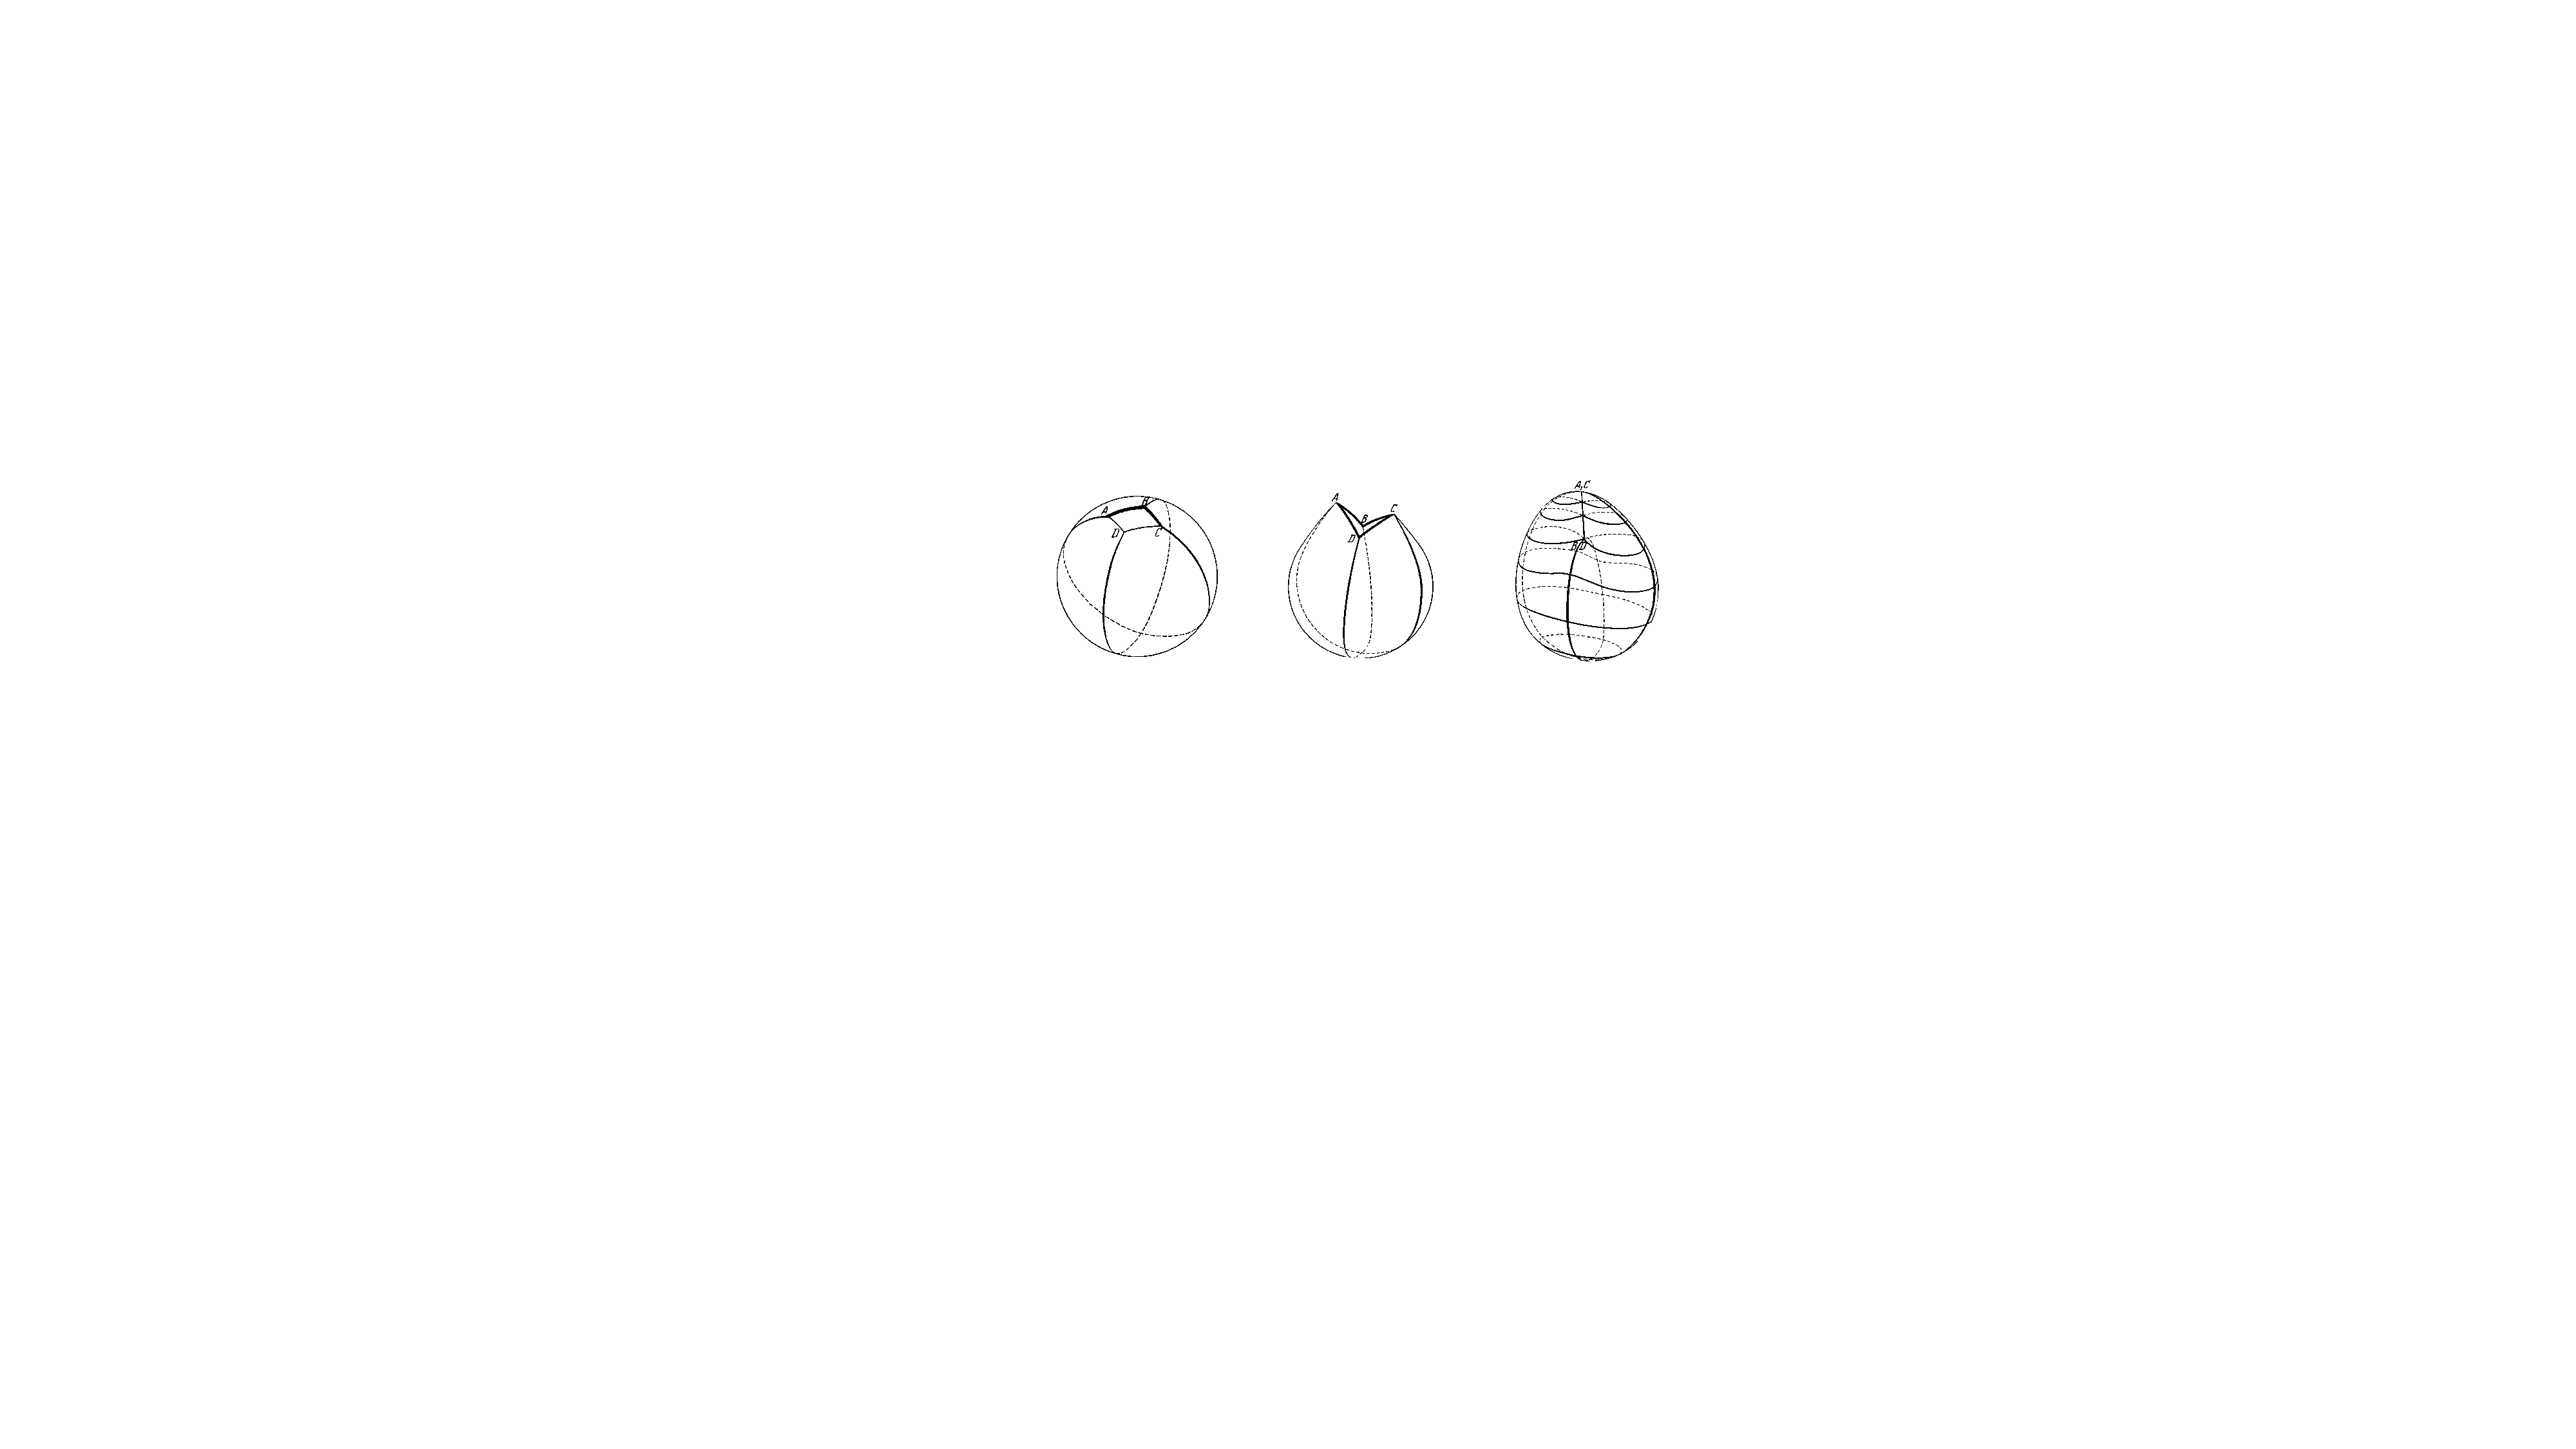
\includegraphics[scale=0.6]{figures/crosscap.pdf}
    \caption{Construction of the projective plane out of a disk. Adding a hole to this surface creates a crosscap, which is homeomorphic to a M\"bius band, see Exercises~\ref{RP2 exercise} and \ref{crosscap exercise}.}
    \label{fig:crosscap}
\end{figure}
\begin{example}{{{\cite[Exercise III.3]{Bredon}}}}
    Consider an annulus. Identify antipodal points on the outer circle. Also identify antipodal points on the inner circle. Calculate the fundamental group of this surface. Is it homeomorphic to any of the orientable compact surfaces? \emph{Hint:} taking $U$ and $V$ to be overlapping annular neighborhoods of the two boundaries of the annulus, the generator of $\pi_1(U\cap V)$ is mapped to the square of the generator in $\pi_1(U)$ and similarly in $\pi_1(V)$; therefore $\pi_1(U\cup V)=\langle a,b\mid a^2=b^2\rangle$.
\end{example}
\begin{xca}[{{\cite[Exercise 1.20]{Hatcher}}}]
    Let $X$ be the subspace of $\bbR^2$ that is the union of the circles $C_n$ of radius $n$ and center $(n, 0)$ for $n = 1, 2, \ldots$. Show that $\pi_1( X )$ is the free group $\ast_n \pi_1( C_n )$, the same as for the infinite wedge sum $\bigvee_{i=1}^\infty \bbS^1$. Show that $X$ and $\bigvee_{i=1}^\infty \bbS^1$ are in fact homotopy equivalent, but not homeomorphic.
\end{xca}

\begin{example}[Hawaiian earring {{\cite[Example~1.25]{Hatcher}}}]\label{hawaiian earring}
    Let $X$ be the subspace of $\bbR^2$ that is the union of the circles $C_n$ of radius $1/n$ and center $(1/n, 0)$ for $n = 1, 2, \ldots$. Initially this space can be mistaken for the infinite wedge sum $\bigvee_{i=1}^\infty \bbS^1$, but in fact it has a much larger fundamental group. This is because in the topology induced from $\bbR^2$ it is possible for a continuous loop $\gamma[0,1]\to X$ to cover an infinite number of circles $C_n$ at once, unlike in the case of the wedge sum. As a result, $\pi_1(X)$ can be mapped surjectively onto the infinite direct product group $\prod_{n=1}^\infty \bbZ$, which is uncountably large. 
\end{example}

\begin{example}[Torus knots {{\cite[Example~1.24]{Hatcher}}}]
    For relatively prime integers $m,n$, the \emph{torus knot}\index{Torus knots}\index{Knot!torus} $K=K_{m,n}\subset \bbR^3$ is the image of the embedding $f:\bbS^1\to \bbS^1\times \bbS^1\cong \bbT^2\subset\bbR^3$ given by $f(z)=(z^m,z^n)$ ($z=\rme^{2\rmi\pi t}$), where the torus $T$ is embedded in space in the standard way. Let us compute $\pi_1(\bbR^3\setminus K)$. First, we can safely replace $\bbR^3$ with its compactification $\bbS^3$ by adding ``a point at infinity''. This isomorphism follows from the Seifert-van~Kampen theorem. Now we may decompose $\bbS^3\setminus \bbT^2$ into two open solid tori $U,V$. Let $C$ be an open tubular neighborhood of $T\setminus K$. Then $U\cup C$ and $V\cup C$ form an open covering of $\bbS^3\setminus K$ with a path connected intersection. The fundamental groups of $U\cup C$, $V\cup C$, and the intersection $C$ are all isomorphic to $\bbZ$ and generated by loops $x,y,z$, respectively. The inclusions of $C$ into $V\cup C$ or $U\cup C$ map $z$ to $x^m$ or $y^n$. Therefore $\pi_1(\bbS^3\setminus K)=\langle x,y\mid x^m=y^n\rangle$. The center of this group is the subgroup generated by the element $x^m=y^n$, and the factor by the center is exactly $\bbZ_m\ast\bbZ_n$. By commuting all powers of $x^m$ through to the left, the elements of this group can be uniquely represented by strings of the form $x^{mk}y^{l_0}x^{k_1}y^{l_1}x^{k_2}y^{l_2}\cdots$ where $k\in\bbZ$, $k_i\in {0,\ldots,m}$ and $l_i\in\{0,\ldots,n\}$.
\end{example}

\begin{example}[Lens spaces {{\cite[Exercise III.10]{Bredon}}}]\label{example Lens space bredon}
    Let $X=(\bbD^2\times \bbS^1)\sqcup_f (\bbD^2\times \bbS^1)$ be the gluing of two solid tori along the map $f:\bbS^1\times \bbS^1\to \bbS^1\times \bbS^1$ induced from the linear map $\bbR^2\to\bbR^2$ given by an integer matrix $\begin{pmatrix}a&b\\c&d\end{pmatrix}$. The fundamental group of a solid torus are generated by one generator, call it $\gamma_1$ and $\gamma_2$ for the two solid tori correspondingly; in addition, the two solid tori overlap by a space that deformation retracts onto a torus $\bbT^2$ whose fundamental group is generated by two simple generators $\alpha$ and $\beta$; assuming $a\neq 0$, by Seifert-van~Kampen, from one inclusion we have the mappings $\alpha\mapsto\gamma_1$ and $\beta\mapsto e$, whereas from the other we get $\alpha\mapsto \gamma_2^d$ and $\beta\mapsto \gamma_2^c$. The resulting identification $\gamma_1\sim \gamma_2^d$ simply allows us to drop $\gamma_1$ from the list of generators. Thus $\pi_1(X)$ is the cyclic group $\langle \gamma_2\mid \gamma_2^c\rangle=\bbZ_c$. Note that the case $a=0$ is special -- in that case $\pi_1(X)=\bbZ$. If the matrix of $f$ is invertible (which is true iff $\det f=\pm1$) and is parametrized as $\begin{pmatrix}q&(qq'-1)/p\\p&q'\end{pmatrix}$, the resulting space is the so called \emph{lens space}\index{Lens spaces} $L(p;q)$ with fundamental group $\bbZ_p$. We have $L(1;0)=\bbS^3$ ($f=\id$) and $L(2;1)=\RP^3$ ($f=-\id$).
\end{example}





\clearpage

\chapter{Manifolds}

\section{Topological manifolds}
\begin{defn}[Locally Euclidean Space]\index{Locally Euclidean Space}
    A topological space $X$ is locally $n$-dimensional Euclidean if every $x\in X$ has an open neighborhood homeomorphic to the open $n$-dimensional ball, $U_x\cong B^n$. 
\end{defn}
\begin{defn}[Second-countability]\index{Second countable space}
    A topological space is called second countable if it has a countable basis of topology.
\end{defn}
\begin{defn}[Paracompactness]\index{Paracompact space}
\begin{enumerate}
    \item A collection of subsets $A_\alpha, \alpha \in I,$ of $X$ is called locally finite if every $x\in X$ has an open neighborhood $U_x$ such that $U_x\cap A_\alpha \neq \varnothing$ only for a finite number of $\alpha$'s. If all $A_\alpha$'s are open, this is the same as $x$ being an element of only finitely many of them.
    \item Given an open covering $\{U_\alpha\}$ (i.e., a collection of open sets such that $\bigcup_\alpha U_\alpha=X$), a refinement of it is an open covering $\{V_\beta \}$ such that $\forall \beta \;\exists \alpha: V_\beta \subset U_\alpha $.
    \item $X$ is called paracompact if every open covering of $X$ admits an open, locally finite refinement.
\end{enumerate}
\end{defn}
\begin{defn}[Topological manifold]\index{Manifold!topological}
    A topological manifold is a second countable, Hausdorff, locally Euclidean space.
\end{defn}
The following proposition is the reason why second countability is often substituted with paracompactness in the definition of manifolds.
\begin{prop}[{{\cite[Thm. 1.15]{Lee}}}]
    All topological manifolds are paracompact (and locally compact).
\end{prop}

\begin{defn}[Charts]\index{Chart}
    Let $X$ be an $n$-dimensional topological manifold. A \emph{chart} on it is a pair $(U,\varphi)$, where $U\subset X$ is an open set and $\varphi:U\to \bbR^n$ is a continuous map (called the chart map) that is also a homeomorphism onto its image $\wh{U}=\varphi (U)$, i.e., $U\cong \varphi(U)=\wh{U}$. The chart is called a \emph{coordinate ball} if $\wh U$ is a ball in $\bbR^n$. The values $\bf{x}=\varphi(x)\in\bbR^n$ of $\varphi$ are called \emph{coordinates} of the corresponding points on $X$. Hence, sometimes we will write $(U,\bf{x})$ to denote the chart.
\end{defn}
\begin{rem}
    Since $X$ is locally Euclidean, every point $x$ automatically has a chart $(U_x,\varphi)$ around it. In particular, every manifold has an open covering by charts $(U_\alpha,\varphi_\alpha)$.
\end{rem}

\begin{thm} All topological manifolds have the following properties.
\begin{enumerate}[label=(\alph*)]
    \item There is a countable basis consisting of coordinate balls (it can also be made locally finite and every ball can be made precompact)
    \item Local compactness.
    \item Local path-connectedness (i.e., every point has a path-connected neighborhood).
    \item At most countably many connected components, each open and a topological manifold of its own.
    \item The fundamental group $\pi_1(X)$ is at most countable.
\end{enumerate}
\end{thm}
\begin{proof}
    (1,2): Pick an open covering by charts $\{U_\alpha\}$. Each $U_\alpha $ can be covered by countably many coordinate balls $V_{\alpha_i}$ because $\wh{U}_\alpha$ can be covered by countably many balls in $\bbR^n$. By second countability, there is a countable subcovering and basis $\{V_\beta\}$. Fixing a chart $U$ and covering it by coordinate balls $V_\alpha$, we have that $\xoverline{V}_\beta$ is compact in $U$ (because it's homeomorphic to a closed ball), therefore closed in $X$ by Hausdorffness. Therefore it's also compact in $X$, i.e., $V_\beta$'s are precompact. The covering can also be made locally finite: let $\{K_i\}_{i=1}^\infty$ be an exhaustion of $M$ by compact sets (i.e., $\bigcup_i K_i=M$; we will prove the existence in Prop. \ref{prop.exhaustion}). After picking out a finite subcovering of every compact ``stripe'' $K_{i+1}\setminus \Int K_{i}$ by charts that are small enough to fit within the wider open ``stripe'' $\Int K_{i+2}\setminus K_{i-1}$ (possible because all charts still form a basis), we end up with a locally finite covering (since every point of the manifold is contained only in 3 of the open stripes).

    (3) is obvious because it holds for balls. (4) follows because second countability implies countable number of components. The rest is obvious. For (5) see \cite[Thm.~1.16]{Lee}.
\end{proof}

\begin{lem}
    Locally path-connected and connected implies path-connected.
\end{lem}
\begin{proof}
    The reverse direction is obvious. In the forward direction, introduce the set $C=\{q:q\text{ is connected with }p\}$  for some fixed $p\in X$. We will prove that $C$ is clopen and therefore equal to $X$.

    $C$ is open because $X$ is locally path-connected.
    $C$ is closed because for any $z\in\xoverline{C}$ there is a path-connected neighborhood $U_z$, thus $U_z\cap C\neq \varnothing$, and $z\in C$. Therefore $\xoverline C=C$. 
    But $X$ is connected, and $C$ is clearly not empty, therefore $C=X$, and lastly $C$ is path-connected by definition.
\end{proof}
\begin{cor}
    For manifolds, connectedness is equivalent to path-connectedness. In particular, connected components of manifolds are path-connected.
\end{cor}

\begin{example}
\begin{enumerate}
    \item Any open set in $\bbR^n$ is a manifold.
    \item $\bbS^n$ is a manifold because it can be covered by finitely many charts $(U_i,\varphi_i)$, where $U_i$ is an open hemisphere whose ``equator'' lies on one of the coordinate hyperplanes, and $\varphi_i$ is simply the orthogonal projection to that hyperplane.
    \item An $n$-dimensional torus $\bbT^n=(\bbS^1)^{\times n}$ is a manifold.
    \item The figure eight, 8, as a subset of $\bbR^2$, is not a manifold, because its center doesn't have a neighborhood homeomorphic to an interval.
    \item Matrices $\Mat(n,\bbR )$ form an $n^2$-dimensional manifold (isomorphic to $\bbR^{n^2}$). So do invertible matrices $\GL(n,\bbR )$ (being an open subset in $\bbR^{n^2}$) and all other classical matrix groups.
\end{enumerate}
\end{example}

\section{Smooth structures}
\begin{defn}[Atlas]\index{Atlas!topological}
    An atlas $\mathcal{A}$ for a topological manifold $M$ is a collection of continuous charts $\{(U_\alpha,\varphi_\alpha)\}$, $\varphi_\alpha:U_\alpha\to \wh{U}_\alpha \subset \bbR^n$ such that $\bigcup_\alpha U_\alpha =M$.
\end{defn}
Throughout these notes we also adopt the notation where for any atlas as above, $U_{\alpha\beta}=U_\alpha \cap U_\beta$, $U_{\alpha\beta\gamma}=U_\alpha \cap U_\beta \cap U_\gamma$, etc.

\begin{defn}[Smooth atlas]\index{Atlas!smooth}
    An atlas is called smooth (or of class $C^k$ or $C^\omega$) if all of the \emph{transition functions} $\varphi_{\beta\alpha}=\varphi_\beta\circ\varphi_\alpha^{-1}:\varphi_\alpha(U_{\alpha\beta})\to\varphi_\beta(U_{\alpha\beta})$ are smooth/$C^\infty$ (of class $C^k$, or real analytic, respectively) in the sense of multivariate calculus on $\bbR^n$.
\end{defn}
\begin{defn}[Equivalent atlases]\index{Atlas!equivalence of}
    Two atlases $\mathcal{A}_1$ and $\mathcal{A}_2$ are called equivalent, or compatible, if $\mathcal{A}_1\cup\mathcal{A}_2$ is still an atlas of the same smoothness class.
\end{defn}
\begin{defn}[Differentiable structure]\index{Differentiable structure}\index{Smooth structure}
    A smooth ($C^k$, analytic) structure on a topological manifold $M$ is an equivalence class $[\mathcal{A}]$ of smooth (respectively, $C^k$, $C^\omega$) atlases on it. 
\end{defn}
\begin{defn}[Smooth manifold]\index{Manifold!smooth}
    A smooth manifold is a pair $(M,[\mathcal{A}])$ consisting of a topological manifold and a smooth structure.
\end{defn}

\begin{rem}
    Recall that the second countability of topological manifolds implies their paracompactness (but not vice versa). In the case of differentiable manifolds, these properties turn out to be equivalent, and also equivalent to metrizability, or to the existence of smooth partitions of unity (see next section). This is why the definitions sometimes differ.
\end{rem}

\begin{rem}
    Given a manifold with one type of structure, e.g., a topological manifold, we might be able to find more special structures compatible with the given one. Compatibility here means that the atlas defining the latter structure is a subset of the former. For example, given a $C^1$-manifold, its atlas might (and, as it turns out, always does) contain a sub-atlas whose transition maps are of class $C^2$. In general there might be multiple non-equivalent sub-atlases of any required type, but a theorem of Whitney shows that every $C^1$-manifold has a unique compatible real analytic structure (a similar statement does not hold for topological manifolds). We will encounter this idea many times throughout this book: fiber bundles, Lie groups, and more general Cartan geometries can all be defined using special atlases compatible with the original structure.
\end{rem}

\begin{example}
\begin{enumerate}
    \item Let $\psi:\bbR \to\bbR $ be $\psi(x)=x^3$. Then $\{(\bbR ,\psi)\}$ is an atlas that defines a smooth structure on $\bbR $. It is not smoothly compatible with the standard smooth structure given by the chart map $\varphi(x)=x$, because the transition function $\varphi\circ \psi^{-1}(x)=x^{1/3}$ is not smooth. Therefore $\bbR $ has many (in fact, infinitely many) different smooth structures.
    \item Any real or complex vector space is automatically a smooth manifold.
    \item Spaces of matrices, classical groups, spheres... are all smooth manifolds with their standard structures.
    \item Not every topological manifold admits a smooth structure, although examples are pretty difficult to construct. On the other hand, any $C^1$ manifold admits a compatible (in the $C^1$ sense) smooth structure, which is unique up to diffeomorphism (see below). This is why even mathematicians are mostly happy working with just either topological or immediately smooth/analytic manifolds. Interestingly, all topological manifolds in dimensions 1,2, and 3 admit unique (up to diffeomorphism) smooth structures.
    \item All Lie groups (defined as smooth manifolds with a group structure in which multiplication and inversion are smooth maps) in fact support a unique (up to diffeomorphism) $C^\omega$ structure. This is an immediate consequence of the convergence of the Baker-Campbell-Hausdorff series, as we will see.
\end{enumerate}
\end{example}

From now on we work only with smooth manifolds, and use the word ``manifold''  to mean ``smooth manifold'' unless otherwise specified.
\begin{defn}[Smooth maps]\index{Smooth map}
    Let $M$ and $N$ be two manifolds with atlases $\{(U_\alpha,\varphi_\alpha)\}$ and $\{(V_\beta,\psi_\beta)\}$, respectively. A map $f:M\to N$ is called smooth if all of its \emph{local representatives} $f_{\beta\alpha}=\psi_\alpha\circ f\circ \varphi_\beta^{-1}:\wh{U}_\beta\to \wh{U}_\alpha$ are smooth. The set of all smooth maps between two manifolds is denoted by $C^\infty (M,N)$. When $N=\bbR $, we write $C^\infty(M)=C^\infty (M,\bbR )$ for the space of ``smooth functions''. The category $\mathsf{Man}^\infty$ is the category of smooth manifolds with smooth maps for morphisms.
\end{defn}
\begin{xca}
    Check that all chart maps in any atlas of a smooth manifold $M$ are smooth as maps from $M$ to the standard $\bbR^n$.
\end{xca}
\begin{rem}
    The above exercise illustrates the general alternative approach to manifolds: instead of defining a smooth structure in terms of charts, we could describe it by specifying \emph{what smooth functions should be} by describing the subsets of the sets of local continuous functions $C(U_\alpha)$ that we want to be smooth (more precisely, one has to pick a subsheaf of the sheaf of continuous functions that is locally isomorphic to the sheaf of smooth functions on $\bbR^n$).
\end{rem}
\begin{defn}[Manifolds with boundaries]\index{Manifold!with boundaries/corners}
    Let $\wb\bbR_+^n$ be the closed upper half-space in $\bbR^n$ (i.e., $x^n\geq 0$). An $n$-dimensional manifold with boundaries is defined just like a smooth manifold, only now some of the chart maps can map to $\wb\bbR_+^n$. The smoothness of boundary transitions is characterized as follows: any function $\wb\bbR_+^n\to \wb\bbR_+^n$ is called smooth if it can be extended as a smooth function into an open neighborhood of $\wb\bbR_+^n$. The set of points of $M$ that map to the boundary of $\wb\bbR_+^n\subset \bbR^n$, i.e., the hyperplane $x^n=0$, is called the boundary $\partial M$. We also denote the interior by $\mathring M=M\setminus \partial M$.
\end{defn}
\begin{example}
    $\sqrt{y}:\wb\bbR_+\to\bbR $ is not smooth on $\wb\bbR_+$ with the standard smooth structure. However, it can be taken to be the chart map defining a new smooth structure on $\wb\bbR_+$, and in that new structure it'll become smooth, because its local representative will be the identity map.
\end{example}
\begin{rem}
    Similarly, one can define \emph{manifolds with corners} using chart maps that can take values in quadrants, octants, and so on, of $\bbR^n$.
\end{rem}

\begin{defn}[Diffeomorphisms]\index{Diffeomorphism}
    A smooth map $f:M\to N$ between manifolds is a called a diffeomorphism if it has a smooth inverse. They are the isomorphisms in $\mathsf{Man}^\infty$.
\end{defn}
\begin{prop}
\begin{enumerate}
    \item Diffeomorphisms are homeomorphisms and open.
    \item If $M$ and $N$ have boundaries and $f:M\to N$ is a diffeomorphism, then $f(\partial M)=\partial N$ and $\restr{f}{\mathring M}: \mathring M\to \mathring N$ is a diffeomorphism.
\end{enumerate}
\end{prop}
\begin{example}
\begin{enumerate}
    \item Different smooth structures can be diffeomorphic! Take $\bbR $ with the chart $\psi(x)=x^3$ that we considered earlier. It is diffeomorphic to the standard smooth structure given by the chart $\varphi(x)=x$, and the diffeomorphism is given by $\psi$ itself! Indeed, its local representative in the two charts is $\varphi\circ \psi \circ\psi^{-1}(x)=x$. In this manner one can show that there is only one smooth structure on $\bbR$ up to diffeomorphism.
    \item Historically the first manifolds to be found to support more than one non-diffeomorphic smooth structure were spheres, starting with $\bbS^7$ which has 28 diffeomorphism classes of smooth structures. These smooth structures are now known as Milnor's \emph{exotic spheres}.
    \item $\bbR^n$ has only one smooth structure up to isomorphism for all $n\neq 4$. For $n=4$, it admits \emph{uncountably many} non-diffeomorphic structures. This makes the study of four-dimensional topological manifolds especially sophisticated, and there are still many very fundamental unsolved problems in four-dimensional topology \cite{smooth.structures}.
    \item In every dimension $n\geq 4$ there exist \emph{compact} topological manifolds that don't admit any compatible smooth structure.
\end{enumerate}
\end{example}

\begin{xca}
    Show that $\bbS^1$ supports only one smooth structure up to diffeomorphism.
\end{xca}






\section{Partitions of unity}

First we note that on $\bbR^n$ there exist bump functions, i.e., for any point $x_0$ and any two radii $0<r_1<r_2$ there is a function $\eta\in C^\infty(\bbR^n)$ such that $\restr{\eta}{B_{r_1}(x_0)}=1$ and $\restr{\eta}{\bbR^n\setminus \overline{B_{r_2}}(x_0)}=0$.
\begin{xca}
    Using the function $\int_a^x \rme^{\frac{1}{(x'-a)(b-x')}} \dd x'$ defined on $(a,b)$, construct a general bump function for $\bbR^n$.
\end{xca}

Now, any manifold $M$ can be covered by a locally finite collection of coordinate balls $(U_\alpha,\varphi_\alpha)$. Let $\eta_\alpha$ be a bump function that equals $0$ outside of the ball $\wh{U}_\alpha\subset \bbR^n$. Then define the smooth functions
\[f_\alpha =\begin{cases} \eta_\alpha\circ\varphi_\alpha, & \text{on }U_\alpha, \\ 0, & \text{on }M\setminus U_\alpha.\end{cases}\]
Finally, we normalize this collection of functions by defining
\[\chi_\alpha(x)=\frac{f_\alpha(x)}{\sum_\alpha f_\alpha (x).}\]
This expression is well-defined because the sum in the denominator is finite for every fixed $x$. These functions have the following properties:
\begin{enumerate}
    \item $\chi_\alpha\in C^\infty(M)$,
    \item $0\leq \chi_\alpha\leq 1$,
    \item $\supp \chi_\alpha\subset U_\alpha$,
    \item $\{\chi_\alpha\}$ is locally finite, i.e., only finitely many of them are nonzero at any given point $x\in M$,
    \item $\sum_\alpha \chi_\alpha (x)\equiv 1$.
\end{enumerate}

\begin{defn}[Partition of unity]\index{Partition of unity}
    Any collection of functions satisfying the above list of properties is called a \gls{pou} subordinate to the open covering (not necessarily by coordinate balls) $\{U_\alpha\}$ of $M$.
\end{defn}

\begin{prop}[{{\cite[Thm.~4.85]{LeeTop}}}]
    Any open covering of a paracompact Hausdorff space admits a subordinate \gls{pou}.
\end{prop}

\begin{prop}
    Any open covering of a smooth manifold admits a subordinate partition of unity.
\end{prop}
\begin{proof}
    Any open covering has a locally finite refinement consisting of coordinate balls, which allows us to apply the construction above to the refinement. Notice that second countability is key to the existence of partitions of unity.
\end{proof}
\begin{thm}[Extension lemma]\label{extension lemma}\index{Extension lemma}
    Let $A\subset M $ be a closed subset, and $f\in C^\infty(A,\bbR^k)$. Then for any open $U$ such that $A\subset U$, there exists an extension $\wt{f}\in C^\infty(M,\bbR^k)$: $\restr{\wt{f}}{A}=f$, such that $\supp \wt{f}\subset U$.
\end{thm}
\begin{proof}
    Pick $p\in A$ and neighborhood $U_p\subset U$. Let $\wt{f}_p: U_p\to\bbR^k$ be a smooth extension of $f$ from $U_p\cap A$. It is guaranteed to exist for sufficiently small $U_p$ by definition of smoothness on closed subsets of $\bbR^n$ and smoothness of chart maps.

    Then $\{U_p\}_{p\in A}\cup \{M\setminus A\}$ is an open covering of $M$. Let $\{\chi_p\}\cup\{\chi_0\}$ be a \gls{pou} subordinate to this covering (and $\chi_p=0$ inevitably for almost all $p$ so that the resulting collection is locally finite). Therefore $\chi_p\cdot \wt{f}_p:U_p\to\bbR^k$ are smooth and vanishing at the boundary of $U_p$, which allows us to extend them by zeros to smooth functions on all $M$. Finally, $\wt{f}=\sum_{p\in A} \chi_p \wt{f}_p$ is the extension we seek with support inside $U$.
\end{proof}
\begin{defn}[Exhaustion function]\index{Exhaustion}
    A function $f\in C^\infty(M)$ is called an exhaustion function for $M$ if for every $c\in\bbR $ the preimage $f^{-1}((-\infty,c])$ is relatively compact (i.e., has compact closure in $M$).
\end{defn}
\begin{prop}\label{prop.exhaustion}
    Every smooth manifold has an exhaustion function.
\end{prop}
\begin{proof}
    Let $\{V_\alpha\}$ be a countable open covering by precompact sets and $\{\chi_\i\}_{i=1}^\infty$ a subordinate \gls{pou}. Define $f(x)=\sum_{n=1}^\infty n\cdot \chi_n(x)$. 

    Clearly $f^{-1}((-\infty,c])\subset \bigcup_{i=1}^{[c]+1}\xoverline{V_i}$, which is a compact set.
\end{proof}







\section{Sard's theorem}

In $\bbR^n$, a set $A$ is said to have\emph{ zero measure} if for any $\epsilon>0$ it can be covered by a collection of open balls $B_i$ such that the total volume of these balls is less than $\epsilon$.

\begin{defn}[Measure zero]
    Even though there is no canonical way to measure volumes on manifolds, there is still a consistent notion of zero measure. Namely, a set $A\subset M$ has zero measure if all the sets $\varphi_\alpha(A\cap U_\alpha)$ are measure zero in $\bbR^n$ for an atlas $\{(U_\alpha,\varphi_\alpha)\}$.
\end{defn}

\begin{defn}[Rank of a map]\label{def.rank}\index{Rank of a map}
    Let $f\in C^\infty (M^m,N^n)$ (superscripts here indicate the dimensions of the manifolds). We say that the rank of $f$ at $p\in M$ is $\rank_p f=r$ if there exist two local charts, $(U,\varphi)$ around $p \in M$ and $(V,\psi)$ around $f(p)\in N$, such that the local representative of $f$ in these charts is $\psi\circ f\circ\varphi^{-1}(x^1,\ldots,x^m)=(x^1,\ldots,x^r,\underbrace{0,\ldots,0}_{n-r})$.
\end{defn}

\begin{defn}[Critical and regular points/values]\index{Critical points/values}\index{Regular points/values}
    $p\in M$ is said to be a critical point of $f\in C^\infty(M^m,N^n)$ if $\rank_p f<n$, i.e.~if its differential at $p$ is not surjective. In this case, $f(p)\in N$ is called a critical value of $f$. Otherwise, $p$ is a regular point, and a regular value is one all of whose preimages are regular points.
\end{defn}

The main property of regular values of smooth maps is that they are generic, as demonstrated by the following deep theorem. We will need this result when we talk about transversality in the context of fiber bundles.

\begin{thm}[Sard]\index{Theorem!Sard}\label{thm sard}
    For any $f\in C^\infty(N,M)$ the set of critical values (also known in some contexts as the \emph{caustic}) of $f$ has measure zero in $M$.
\end{thm}
\begin{proof}
    This theorem is essentially entirely local, i.e., it suffices to prove it for $N=\bbR^n$ and $M=\bbR^m$. Every manifold can be broken up into a countable number of neighborhoods, and a countable union of sets of measure zero is still measure zero.

    Let $C\subset \bbR^m$ be the set of critical points of $f:\bbR^n\to \bbR^m$ and pick $x_0\in C$. Then, after some rotation of the space, we can assume that its derivative maps $f'_{x_0}(\bbR^n)=\bbR^k\times \{0\}\subset \bbR^m$, where $k\leq n-1$ is the rank of the Jacobi matrix at $x_0$.  If we choose a ball $B_r(x_0)$ of radius $r$ around $x_0$, then
    \[f'_{x_0}(B_r(x_0))\subset (\bbR^k\times \{0\})\cap B_\epsilon(f(x_0)),\quad \epsilon=r\cdot \mathrm{Lip}f,\]
    where $\mathrm{Lip}f$ is the Lipschitz constant of $f$ inside $B_r(x_0)$ (equal to the supremum of all directional derivatives in unit directions). We only need the existence of such an $\epsilon$ and that it goes to zero with $r\to 0$.

    Therefore $f'_{x_0}(B_r(x_0))$ can be covered by $N^k$ cubes of diameter $\epsilon/N$. By differentiability there exists $\delta>0$ such that 
    \[\lvert f(y)-f(x_0)-f'_{x_0}(y-x_0)\rvert\leq \frac{1}{N}|y-x_0|,\quad \text{ for all }y\in B_\delta(x_0).\]
    So $f(y)$ is within $r/N$ distance of the hyperplane $f(x_0)+f'_{x_0}(\bbR^n)$ (provided that $r<\delta$). Therefore the image $f(B_r(x_0))$ itself is contained in a neighborhood of $f'_{x_0}(B_r(x_0))$ of radius $r/N$. Thus we can construct $N^k$ disjoint sets $E_j$ of diameter $\sim r/N$ that cover $f(B_r(x_0))$.

    We repeat the above for every point $x\in C$ and get $r_x>0$ such that $f(B_{r_x}(x))\subset \bigsqcup_{j=1}^{N^k}E_j^x$. By \href{https://en.wikipedia.org/wiki/Vitali_covering_lemma}{Vitali's covering lemma}, there is a countable subcovering, so $C\subset \bigsqcup_{i=1}^\infty B_{r_i}(x_i)$ such that $\{B_{r_i/5}(x_i)\}$ are disjoint and for every $i$ there are sets $E^i{}_j,j=1,\ldots,N^k$ such that $\mathrm{diam}(E^i{}_j)\sim r/N$ and $f(B_{r_i}(x_i))\subset \bigsqcup_{j=1}^{N^k}E^i{}_j$. Thus $f(C)\subset \bigsqcup_{i=1}^\infty\bigcup_{j=1}^{N^k}E_j^i$. We can safely assume that $C\subset [-l,l]^n$ for some $l\in \bbN$ (otherwise it can be broken up into countably many pieces of this kind, which won't upset the result of the theorem). By compactness we can then assume that $r_x<1$ for all $x\in C$. Thus
    \begin{multline}
        \mathrm{volume}(f(C))\leq \sum_{i,j}(\mathrm{diam}(E^i{}_j))^n\leq \sum_{i,j}\left(\frac rN\right)^n\lesssim \sum_{i}N^k\frac{r^n}{N^n}\lesssim \\
        \lesssim 5^nN^{k-n}\sum_i\frac{r^n}{5^n}\lesssim 2\cdot 5^n N^{k-n}\cdot \mathrm{volume}([-l,l]^n),
    \end{multline}
    since $C$ lies inside $[-l,l]^n$ and is covered by balls of radii $r_i\leq 1$ with disjoint sub-balls, so the sum of the volumes of these sub-balls can only exceed the volume of $[-l,l]^n$ by at most a constant factor (coming from pieces that stick out of $[-l,l]^n$), say $2$.

    But now, $k<n$, thus in the limit $N\to \infty$ we find that the volume of $f(C)$ has to be zero. This proof is due to Behnam Esmayli, a more conventional one can be found in \cite[Thm.~6.10]{Lee}.
\end{proof}
\begin{rem}
    The ability to globalize the proof of this theorem depends crucially on second countability. Indeed, we could consider a non-second-countable $1$-dimensional ``manifold'' given by the uncountable disjoint union of lines $M=\bigsqcup_{a\in \bbR} R_a=\bigsqcup_{a\in \bbR} \bbR$ (so called \emph{long line}\index{Long line}), and define a function $f:M\to \bbR$ by $\restr{f}{R_a}=a$. In this case $f$ is smooth and every value $a\in\bbR$ is a critical value, contrary to Sard's theorem. This violates the setting of the theorem because we found an uncountable family of local neighborhoods ($R_a$), for each of which the set of critical values has measure zero (one point $a$). But the union of an uncountable number of sets of measure zero can have nonzero measure. Thus, second countability is key to Sard's theorem working on general manifolds.
\end{rem}






\section{Inverse \& Implicit Mapping Theorems}

In this \sect\ we just recall the statements of two basic theorems of multivariate calculus.
\begin{thm}[\gls{inmt}]\label{InMT}\index{Theorem!Inverse mapping}
    Let $U,V\subset\bbR^n$ be open and $f\in C^\infty(U,V)$. If the Jacobi matrix $\frac{\partial f^i}{\partial x^j} (\bf{a})$ is invertible for some $\bf{a}\in U$, then there are neighborhoods $\bf{a}\in U_{\bf{a}}\subset U$ and $f(\bf{a})\in V_{f(\bf{a})}\subset V$ such that $\restr{f}{U_{\bf{a}}}:U_{\bf{a}}\to V_{f(\bf{a})}$ is a diffeomorphism.
\end{thm}
Meaning: any smooth map whose Jacobi matrix is non-singular at a point is locally a diffeomorphism around that point.

\begin{thm}[\gls{immt}]\label{ImMT}\index{Theorem!Implicit mapping}
    Let $U\subset \bbR^n\times \bbR^k$ be open, $(\bf{x},\bf{y})=(x^1,\ldots,x^n,y^1,\ldots,y^k)\in U$. Let $\Phi\in C^\infty(U,\bbR^k)$ (with components $\Phi^j$) and $\Phi(\bf{x},\bf{y})=\bf{c}$ for all $(\bf{x},\bf{y})\in U$. If the matrix $\left(\frac{\partial\Phi^i}{\partial y^j}(\bf{y},\bf{x})\right)_{i,j=1}^k$  is non-singular, then there are open neighborhoods $\bf{x}\in V_{\bf{x}}\subset \bbR^n$ and $\bf{y}\in W_{\bf{y}}\subset\bbR^k$ and a smooth map $f\in C^\infty (V_{\bf{x}},W_{\bf{y}})$ such that 
\[\forall\,(\bf{v},\bf{w})\in V_{\bf{x}}\times W_{\bf{y}},\;\; \Phi (\bf{v},\bf{w})=\bf{c} \Leftrightarrow \bf{w}=f(\bf{v}).\]
\end{thm}
Meaning: the equation $\Phi(\bf{x},\bf{y})=\bf{c}$ can be locally solved for $\bf{y}=\bf{y}(\bf{x})$ if the matrix $\partial \Phi/\partial\bf{y}$ is invertible.

\begin{comment}
\PRLsep
\begin{center}
  {\red Lecture 5 on 7 Dec 2018 ended here}
\end{center}
\end{comment}

\section{Tangent spaces}
    In $\bbR^n$, vectors don't have ``base points'' because they can always be parallel transported to the origin. On a manifold, this is impossible without additional structure, which is why there is a tangent space ``attached'' to every point $p\in M$. 
\begin{defn}[Tangent vector I]\index{Tangent vector}\index{Vector}
    Let $m\in M$. If $m\in \mathring M$, consider all curves $\gamma\in C^\infty((-1,1),M)$ such that $\gamma(0)=m$. If $m\in \partial M$, consider instead all curves with domains $(-1,0]$ or $[0,1)$. Introduce the equivalence relation $\gamma_1\sim \gamma_2$  iff $\restr{\frac{\dd}{\dd t}}{t=0}(\varphi_\alpha\circ \gamma_1)(t)=\restr{\frac{\dd}{\dd t}}{t=0}(\varphi_\alpha\circ \gamma_2)(t)$ for any chart $\varphi_\alpha$ around $p$. A tangent vector at $x$ is an equivalence class $[\gamma]_m$ of curves passing through $m$. The set of all tangent vectors at $m$ is denoted by $\T_m M$.
\end{defn}

\begin{enumerate}
    \item $T_m M$ is imbued with the structure of a real vector space as follows:
    \begin{enumerate}
        \item $\lambda\cdot [\gamma(t)]_m\coloneqq [\gamma(\lambda t)]_m$ for $\lambda\in\bbR $.
        \item $[\gamma_1(t)]_m+[\gamma_2(t)]_m\coloneqq [\varphi_\alpha^{-1}(\varphi_\alpha(\gamma_1(t))+\varphi_\alpha(\gamma_2(t)))]_m.$
    \end{enumerate}
    \item We will show later that $\dim \T_m  M=\dim M$.
\end{enumerate}


\begin{defn}[Tangent vector II]
    $\T_m  M$ can be alternatively defined as the set of all \emph{derivations}\index{Derivation} at $m$, i.e., linear functionals $v:C^\infty(M)\to \bbR $ such that $v[f\cdot g]=f(m)v[g]+g(m)v[f]$. This is obviously a vector space. Notably, this definition doesn't need to be modified if $m\in\partial M$.
\end{defn}

\begin{prop}
    The two definitions of tangent spaces given above are isomorphic as vector spaces.
\end{prop}
\begin{proof}
    An explicit linear isomorphism between the two constructions is $[\gamma]_m\mapsto v[f]=\restr{\frac{\dd}{\dd t}}{t=0}f(\gamma(t))$ (this is called the \emph{directional derivative} along the tangent vector $[\gamma]_m$). 

    All derivations on the algebra of smooth functions can be shown to be directional derivatives, which allows us to invert this mapping. Namely, for a chart map $\varphi_\alpha$, the $n$ numbers $v[\varphi_\alpha^i]$ are components of a vector $\wh{v}\in \bbR^n$. Now we can let $\wh{\gamma}(t)=\varphi_\alpha(m)+t\wh{v}$ and $\gamma(t)=\varphi_\alpha^{-1}(\wh{\gamma}(t))$. It is easy to show that this is a linear inverse to the above mapping.
\end{proof}


\begin{xca}
    Check that the definition of a tangent vector and all of the following constructions are consistent, i.e., independent of the choices of charts $\varphi_\alpha$ or representatives $\gamma(t)$ of equivalence classes.
    \end{xca}
    \begin{defn}[Differential/push-forward]\index{Push-forward}
    Let $F\in C^\infty(M,N)$ and $p\in M$. The push-forward, or the \emph{derivative}, of $F$ at $m$ is the linear map $F_{\ast m}:T_m M\to T_{F(m)} N$ defined via \[F_{\ast m}([\gamma]_m)=[F\circ\gamma]_{F(m)},\] or equivalently \[F_{\ast m}(v)[f]=v[f\circ F]\] for any $f\in C^\infty (N)$.
\end{defn}

\begin{rem}[Coordinate expressions for derivatives]
    In local coordinates (i.e.~replacing $F$ with some function $\wh{F}:\bbR^m\to\bbR^n$,
    \[F_{\ast m}([\gamma]_m)=\restr{\frac{\dd}{\dd t}}{t=0} \wh{F}(\gamma(t)).\label{eq differential in local coordinates}\]
    and 
    \[\wh{F}_{\ast m}(v)[f]=\restr{\frac{\dd}{\dd t}}{t=0}f(F(\gamma(t)).\]
\end{rem}


\begin{thm}\label{prop of push-forwards}
    Consider smooth maps between manifolds $M\overset{f}{\to}N\overset{g}{\to}P$. Then
\begin{enumerate}
    \item $f_{\ast m}:\T_m M\to \T_{f(m)} N$ is linear;
    \item $(g\circ f)_{\ast m}=g_{\ast f(m)}\circ f_{\ast m}$ (chain rule);
    \item $(\id_M)_{\ast m}=\id_{\T_m M}$;
    \item if $f$ is a local diffeomorphism at $x$ then $f_{\ast m}$ is invertible and $(f_{\ast m})^{-1}=(f^{-1})_{\ast m}$ (the converse is also true by \gls{inmt});
    \item In local coordinates, $f_{\ast m}$ is represented by the Jacobi matrix of the local representative $f_{\beta\alpha}$;
    \item $\dim T_m M=\dim M$, even for points on $\partial M$;
    \item \gls{inmt} doesn't hold at the boundary.
\end{enumerate}
\end{thm}
\begin{proof}
    The first few statements are trivial and are left as an exercise.
    6) A local chart map $\varphi_\alpha$ can be viewed as a local diffeomorphism to an open subset of $\bbR^n$. Since $T_{\varphi_\alpha(m)}(\bbR^n)=\bbR^n$ (because we know that equivalence classes of curves at a point of $\bbR^n$ are uniquely characterized by their tangent vectors), we have a linear map $(\varphi_\alpha)_{\ast m}:\T_m M\to \bbR^n$, which is an isomorphism by 4). Therefore the dimensions coincide. Nothing really changes at the boundary.

    7) Consider the inclusion map $i:\wb\bbR^n_+\hookrightarrow \bbR^n$. Clearly $i_{\ast 0}=\id$ is invertible, but $i$ itself is not a local diffeomorphism because $i(B^n\cap \wb\bbR^n_+)$ is the image of an open set that is not open in $\bbR^n$.
\end{proof}

All of this implies that the map $\T_m:(M,m)\mapsto \T_m M$ extends to a covariant functor $\T_m:\mathsf{Man}_\bullet^\infty\to \mathsf{Vect}_\bbR$. It respects morphisms (smooth maps) $f:M\to N$ between pointed\footnote{The requirement that these manifolds be pointed is a mere technicality for the sake of the definition of a functor. Given a map $f:M\to N$ and a point $f\in M$, we can always create the pairs $(M,m)$ and $(N,f(m))$ and treat $f$ as a pointed map.} manifolds because the following diagram commutes:
\[
\begin{tikzcd}[every matrix/.append style={name=m},   
    execute at end picture={\draw [<-] ([xshift=-2.6em,yshift=1mm]m-2-2.north) arc[start angle=-90,delta angle=270,radius=0.25cm];}]
   M \arrow[r,"f"]\arrow[d,swap,"\T_m"]& N\arrow[d,"\T_{f(m)}"] \\
   \T_m M\arrow[r,swap, "\T_m  f"]& \T_{f(m)}N.
\end{tikzcd}
\]

As we will show later, the tangent space over $m\in M$ in a certain sense ``varies smoothly with $m$'' and together all of the tangent spaces comprise a single object called the \emph{tangent bundle}. A similar thing happens to the functors $\T_m$.

\section{Rank}
We have defined rank in Definition~\ref{def.rank}. However, that definition is not practical because it's an existence statement rather than a constructive ``measurement''.

Recall that for a matrix $A\in \Mat(n\times m,\bbR )$ its rank $\rank A$ is defined as the maximal number of linearly independent columns (equivalently, rows) in it. More abstractly, the rank of a linear operator is the dimension of its image, $\rank A=\dim(\im (A))$. The following theorem establishes the equality between the rank of a smooth map and the rank of its differential.

\begin{thm}[Rank theorem]\index{Rank theorem}\label{Rank thm}
    For $f\in C^\infty(M,N)$, $\rank_m f=\rank (f_{\ast m})$.
\end{thm}
\begin{proof}
    This is the \gls{inmt} in disguise. Since this theorem is local, we can safely replace $M$ and $N$ by open domains $U\subset \bbR^k$ and $V\subset \bbR^n.$

    Assume $\rank(f_{\ast m})=r$. Introduce coordinates $(x^1,\ldots,x^r$, $y^1,\ldots,y^{k-r})$ on $U$ and $(v^1,\ldots,v^r$, $w^1,\ldots,w^{n-r})$ on $V$. In these coordinates, we can write \[f(x,y)=(F(x,y),G(x,y)).\] \Gls{wlog}, $m=0$, $f(m)=0$, and  $F_{\ast (0,0)}$ is a nonsingular square matrix.

    Define $\varphi:U\to\bbR^m$ by $\varphi(x,y)=(F(x,y),y)$. Its differential at $(0,0)$ is nonsingular by assumption, so by the \gls{inmt} we locally have an inverse and by definition of $\varphi$, the composition of $\varphi^{-1}$ with $f$ will have the form 
    \[
    f\circ\varphi^{-1}=(x,\wt{G}(x,y)).
    \]
    Finally, by a trivial change of coordinates $\psi(v,w)=(v,w-\wt{G}(v,0))$ we can bring the local form of $f$ to \[\psi\circ f\circ \varphi^{-1}(x,y)=(x,0),\] which means that $\rank_m f=r$. The converse direction is obvious.
\end{proof}

\begin{prop}\label{domain of maximal rank}
    For any smooth map $f\in C^\infty (M,N)$ the set of points $m\in M$ where the rank is maximal, i.e., $\rank_m f=\min(\dim M,\dim N)$, is open in $M$.
\end{prop}
\begin{proof}
    Let $\dim M=k$ and $\dim N=n$. The mapping $D:m\mapsto \wh{f}_{\ast m}$ is a continuous (in fact, smooth) map $U_\alpha\subset M\to \Mat(n\times k,\bbR )$. The subset of all matrices of maximal rank is open in $\Mat(n\times k,\bbR )$ (essentially because small perturbations can't make linearly independent vectors dependent\footnote{The converse is not true, which is why the set of matrices of any fixed non-maximal rank is not open.}). By continuity of $D$, the set of $m$ at which the rank is maximal is also open (in every $U_\alpha$ and thus in all of $M$).
\end{proof}

Therefore we see that maps of maximal rank are of special significance. Moreover, they fall into two categories: if $\dim M\leq \dim N$, then the maximal rank equals $\dim M$; if $\dim M\geq \dim N$, the maximal rank is $\dim N$. In the first case, matrices of maximal rank are exactly the injective ones, whereas in the second case they are the surjective ones.

\begin{defn}[Smooth immersions and submersions]
    Among all maps of \emph{constant rank} we single out two special classes.\index{Immersion!smooth}\index{Submersion!smooth}
\begin{enumerate}
    \item $f\in C^\infty(M,N)$ is called an immersion if $f_{\ast m}:\T_m  M\to \T_{f(m)} N$ is injective for all $m$. Equivalently, $f$ is an immersion iff it has everywhere maximal rank and $\dim M\leq \dim N$.
    \item $f\in C^\infty(M,N)$ is called a submersion if $f_{\ast m}:\T_m  M\to \T_{f(m)} N$ is surjective for all $m$. Equivalently, $f$ is a submersion iff it has everywhere maximal rank and $\dim M\geq \dim N$.
\end{enumerate}
\end{defn}

\begin{rem}
    As is clear from Theorem~\ref{Rank thm}, a submersion is a map that is locally an orthogonal projection onto a subspace (in some coordinates), and an immersion is one that is locally an inclusion as a lower-dimensional subspace. A map that is both a submersion and an immersion is a local diffeomorphism. Note that ``locality'' here is understood both in domain and in range -- we have to pick out open neighborhoods of both $m$ and $f(m)$. An immersion for which this property holds globally on the entire domain (i.e.~locally only in the target manifold) is just an injective immersion. Meanwhile, the attempt to define maps that are ``projections locally in the target'' will lead us to the concept of fiber bundles, and it will not be enough for them to be surjective submersions.
\end{rem}


\begin{thm}[Global rank theorem]\label{Global rank}\index{Rank theorem!global}
Let $f\in C^\infty(M,N)$ have constant rank $r$. Then
\begin{enumerate}
    \item if $f$ is injective, it is an immersion;
    \item if $f$ is surjective, it is a submersion;
    \item if $f$ is bijective, it is a diffeomorphism.
\end{enumerate}
\end{thm}
\begin{proof}
\begin{enumerate}
    \item Suppose it is not an immersion. Then $r<\dim M$, which means that in some coordinates we have $\wh{f}(0,\ldots,0,\epsilon)=(0,\ldots,0)$ for all sufficiently small $\epsilon$. This contradicts injectivity.
    \item Suppose it is not a submersion. Then $r<\dim N$. There exists a (countable) open covering  $\{U_\alpha\}$ of $M$ such that $f(U_\alpha)$ are ball-slices $B^n\cap \{y^{r+1}=y^{r+2}=\cdots=y^n=0\}$. We have $f(M)=\cup_\alpha f(U_\alpha)$, but at the same time $f(U_\alpha)$'s are \emph{nowhere dense} (i.e., closure has empty interior). By \href{https://en.wikipedia.org/wiki/Baire_category_theorem}{Baire category theorem}, a countable union of nowhere dense sets has an empty interior, which implies $\Int  f(M)=\varnothing$. This contradicts surjectivity, because $\Int  N\neq\varnothing$.
    \item Obvious (a bijective local diffeomorphism is a diffeomorphism).
\end{enumerate}
\end{proof}



\section{Immersions and embeddings}

\begin{figure}
    \centering
    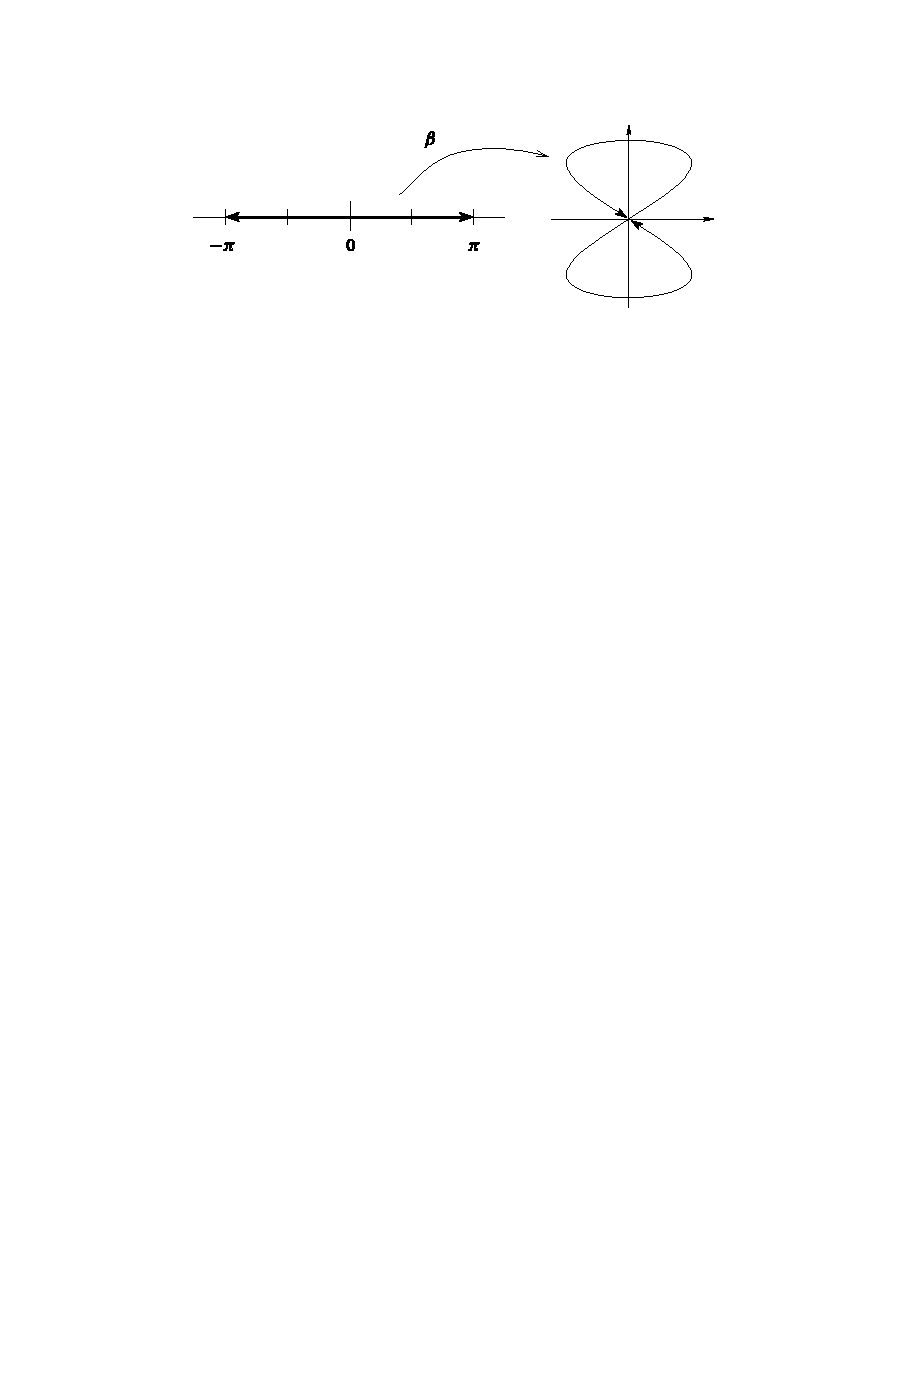
\includegraphics{figures/immersion.pdf}
    \caption{The figure-eight curve $\beta:(-\pi,\pi)\to \bbR^2$ given by $\beta(t)=(\sin 2t,\sin t)$ is an immersion but not an embedding. Its domain is open but its image is closed.}
    \label{fig:immersion}
\end{figure}

As we described above, immersions are maps with injective differentials. Immersions themselves don't need to be injective, and even if they are, their images, as topological subspaces of the codomain, are not even always homeomorphic to the domain. For example, the map in Figure~\ref{fig:immersion} is an immersion whose image is not homeomorphic to the domain. Maps that do respect subspace topology in this way are called embeddings.

In the topological category, the situation is different. A topological immersion is the intuitive analog of the smooth immersion: the injectivity of differentials is replaced by a local homeomorphism property on the domain. 

\begin{defn}[Topological immersion]\index{Immersion!topological}
    A continuous map $f:X\to Y$ is called a topological immersion if for every $x\in X$ there is an open neighborhood $U\subset X$ of $x$ such that $\restr{f}{U}\to f(U)$ is a homeomorphism, where $f(U)$ is taken to have the subspace topology inherited from $Y$.
\end{defn}

A topological embedding then is a global version of a topological immersion: the entire map has to be a homeomorphism onto the image. In particular, it has to be injective.

\begin{defn}[Topological embedding]\index{Embedding!topological}
A topological embedding is a continuous map $f:X\to Y$ that is a homeomorphism onto its image (where the image $f(X)\subset Y$ is taken to have the subspace topology in the target). In other words, it is an injective map such that the topology on the domain must coincide with the initial topology induced by the map.
\end{defn}


In this way the concept of a topological embedding map is dual to that of a topological quotient maps. In the smooth category the picture is a bit different. First, the intuitive smooth version of a quotient map is a smooth submersion that is a topological quotient map. However, as we will see in \S\ref{sec: submersions}, every smooth submersion is automatically a quotient map, so the second requirement can be dropped. On the other hand, smooth immersions are not always topological embeddings (although they are topological immersions). This is why smooth submersions and smooth immersions are not dual concepts, but instead the concept dual to smooth submersions is the following concept of a smooth embedding.

\begin{defn}[Smooth embedding]\index{Embedding!smooth}
A smooth embedding is a smooth immersion that is topological embedding.
\end{defn}

\begin{example}
\begin{enumerate}
    \item Much like the example in Figure~\ref{fig:immersion}, the mapping of $\bbS^1$ onto a figure eight in $\bbR^2$ can be represented by a parametric map $f(t)=(f_x(t),f_y(t))$. It is an immersion provided that $f'(t)$ doesn't vanish anywhere. However, it is not an embedding because the image (figure eight) is not homeomorphic to the circle.
    \item Excluding the one point on the circle that is mapped to the center point of the figure eight in the last example, we obtain a map $f:(0,1)\to \bbR^2$ whose image is still the whole figure eight. This is an injective immersion. However, it is still not an embedding because the image is compact in the subspace topology, whereas the open interval is not a compact space.
    \item $\gamma:\bbR \to \bbT^2$ given by $\gamma(t)=(\rme^{2\pi\rmi t},\rme^{2\pi\rmi \alpha t})$ for $\alpha\in\bbR \setminus\mathbb{Q}$ is an injective immersion. However, its image is dense in the torus, which means that its subspace topology is very different from that of the real line. Namely, there exist convergent sequences of points in the image whose preimages don't converge on the real line. This means that $\gamma^{-1}$ is not continuous and $\gamma$ is not an embedding.
    \item The map $f(x)=(0,x^3)$ is a topological embedding $\bbR \hookrightarrow\bbR^2$ but not a smooth embedding because its differential has rank zero at $x=0$. Essentially this restriction insures that smooth structures induced via smooth embeddings coincide with the original ones. The smooth structure induced via $(0,x^3)$ from $\bbR^2$ (with the standard structure) would give one of the non-standard smooth structures on $\bbR $.
\end{enumerate}
\end{example}

\begin{prop}[{{\cite[Prop.~4.22]{Lee}}}]
An injective immersion $f\in C^\infty (M,N)$ is a smooth embedding if any of the following hold:
\begin{enumerate}
    \item $f$ is open or closed;
    \item $f$ is proper;
    \item $M$ is compact;
    \item $\partial M=\varnothing$ and $\dim M=\dim N$.
\end{enumerate}
\end{prop}

\begin{thm}[Local embedding theorem {{\cite[Thm.~4.25]{Lee}}}]\label{thm.local embedding}
$f\in C^\infty (M,N)$ is an immersion iff it is a local embedding (i.e., every point in $M$ has a neighborhood on which the restriction of $f$ becomes an embedding). 
\end{thm}

\begin{comment}
\PRLsep
\begin{center}
  {\red Lecture 6 on 15 Dec 2018 ended here}
\end{center}
\end{comment}



\section{Submanifolds}
Immersions and embeddings give rise to the notions of immersed and embedded submanifolds.

\begin{defn}\index{Submanifold!immersed}\index{Submanifold!embedded}\index{Submanifold!weakly embedded}\index{Submanifold!initial}\index{Submanifold!properly embedded}
Let $S$ and $M$ be smooth manifolds and let $i:S\to M$ be a continuous map. This triple $S\overset{i}{\to}M$ is called:\index{Submanifold}
\begin{enumerate}
    \item an immersed submanifold if $i$ is a smooth immersion. We write $S<M$.
    \item  a weakly embedded submanifold, or \emph{initial}, if it is immersed and every smooth map $f:N\to M$ such that $\im f\subset S$ restricts in the codomain to a smooth map $f:N\to S$.
    \item an embedded submanifold if $i$ is a smooth embedding map. Often $S\subset M$ with the subspace topology. Then $i$ is required to be a only a topological embedding (and a smooth structure on $S$ can be induced via $i$). We write $S\sub M$.
    \item a properly embedded submanifold if $i$ is a proper smooth embedding map. We write $S\sube M$.
\end{enumerate}
The codimension \index{Codimension} of a submanifold is defined as $\codim S=\dim M -\dim S$.
\end{defn}

Note that sometimes immersed ``submanifolds'' are defined as images of arbitrary immersions, but we avoid that definition since such subsets generally don't admit any manifold structure (since they can self-intersect).

\begin{example}\label{example submanifolds}
\begin{enumerate}
    \item Any open subset is a codimension zero embedded submanifold.
    \item If $F:M\to N$ is an embedding, then $F(M)\sub N$ in the subset sense. i.e., embedded submanifolds inside $N$ are exactly the images of embedding maps.
    \item If $S\sub M$ as a subset, then $S$ is closed iff $S\sube M$.
    \item If $S\sub M$ and $S$ is compact, then $S\sube M$.
    \item  The figure eight immersion $t\mapsto (\sin 2t,\sin t)$ is a weak embedding but not an embedding.
    \item If $f\in C^\infty(N,M)$, then its graph $\mathrm{graph}(f)\subset N\times M$ is an embedded submanifold.
\end{enumerate}
\end{example}


\begin{prop}[{{\cite[Prop.~5.18]{Lee}}}]\label{prop 5.18 Lee}
    If $F:M\to N$ is an injective smooth immersion, then $F(M)$ has a unique topology and smooth structure such that it is a smooth submanifold of $N$ and such that $F:M\to F(M)$ is a diffeomorphism onto its image.
\end{prop}
\begin{proof}
    The topology and smooth structure on $F(M)$ are induced by $F$ itself (i.e.~$U\subset N$ is open iff $F^{-1}(U)\subset M$ is open, and the charts on $F(M)$ are $(F(U),\varphi\circ F^{-1})$ for every chart $(U,\varphi)$ on $M$), and they obviously turn $F$ into a diffeomorphism onto its image, and these are the only topology and smooth structure with this property. The inclusion $F(M)\hookrightarrow N$ can be written as a composition $F(M)\overset{F^{-1}}{\to}M\overset{F}{\to}N$. As a composition of a diffeomorphism and a smooth immersion, it is a smooth immersion.
\end{proof}


\begin{prop}[Slice charts {{\cite[Thm.~5.8]{Lee}}}]\index{Slice chart}
    A subset $S\subset M$ is an embedded submanifold iff every point $m\in S$ has a local \emph{slice chart}, that is, a local chart map $\varphi$ on a neighborhood $U_m\subset M$  such that its image is a slice ball: $\varphi(S\cap U_m)=\{(x^1,\ldots,x^k,0,\ldots,0)\}$, where $k$ is a fixed number called the \emph{dimension} of $S$. In particular, given the existence of slice charts, there is a unique smooth structure on $S$ (given by a codomain restriction of the slice atlas) compatible with the subset topology such that $S\sub M$.
\end{prop}
\begin{proof}
    It suffices to check that slice charts, whose existence was proved above, form a smooth atlas on $S$. This also proves that, given a topologically embedded submanifold $S$ in a smooth manifold $M$, one can induce a smooth structure on $S$, essentially by defining the slice atlas. See the cited reference for full details.
\end{proof}


\begin{cor}
    $\partial M$ has slice charts by definition, therefore it is an embedded submanifold.
\end{cor}

\begin{prop}
    An embedded submanifold  $S\subset M$ is properly embedded iff it is a closed subset of $M$.
\end{prop}
\begin{proof}
    Exercise.
\end{proof}

\begin{thm}[Level Set Theorem]\index{Theorem!Level set}\label{thm level set submanifold}
    If $f\in C^\infty(M,N)$ has constant rank $r$ then the level set $f^{-1}(q)$ for any $q\in N$ is a properly embedded codimension $r$ submanifold.
\end{thm}
\begin{proof}
    By definition of rank, there are coordinates in which the local representative is $\wh{f}(x^1,\ldots,x^n)=(x^1,\ldots,x^r,0,\ldots,0)$. Therefore, assuming $q$ is the origin of its coordinate system, $f^{-1}(q)=(0,\ldots,0,\underbrace{y^1,\ldots,y^{n-k}}_{\text{arbitrary}})$. This means that $f^{-1}(q)$ is a local ball slice and therefore an embedded submanifold. It is closed as a preimage of a closed set under a continuous map, and therefore properly embedded.
\end{proof}
\begin{cor}
    Each level set of a smooth submersion $f:M\to N$ is properly embedded and of dimension $\dim N$.
\end{cor}
\begin{cor}[Regular level set theorem]
    Every regular level set (i.e., level set of a regular value) of a smooth map $f:M\to N$ is a properly embedded submanifold of codimension $\dim N$.
\end{cor}
\begin{proof}
    Since the set of all regular points, being the set of points where $f_{\ast}$ has maximal rank, is open (Proposition~\ref{domain of maximal rank}), the level set is contained in it together with an open neighborhood $U$ of itself: $f^{-1}(q)\subset U\subset M$. Then $\restr{f}{U}$ is a smooth submersion and we can use the last Corollary.
\end{proof}

\begin{prop}
\begin{enumerate}
    \item All embedded submanifolds $S\subset M$ have local defining functions, i.e., $\varphi:C^\infty((U\subset M, \bbR )$ such that $\varphi^{-1}(0)=S\cap U$.
    \item An immersion is a local embedding (i.e., its restriction to a sufficiently small neighborhood $U\subset S$ of a point $m\in S$ is an embedding\footnote{Not true for sufficiently small neighborhoods $V\subset M$ of $m\in S\subset M$ that the restriction of the immersion to $S\cap V$ becomes an embedding!}).
\end{enumerate}
\end{prop}
\begin{proof}
\begin{enumerate}
    \item Take a local slice chart such that $\restr{S}{U}=\{(x^1,\ldots,x^k,0,\ldots,0)\}$ and define $\varphi=(x^{k+1})^2+\cdots+(x^m)^2$.
    \item By Theorem~\ref{thm.local embedding}.
\end{enumerate}
\end{proof}

\begin{thm}[Extensions of functions]
\begin{enumerate}
    \item If $S\sub M$ as a subset, then any $f\in C^\infty(S)$ can be extended to a $\wt f\in C^\infty(U)$ for some open neighborhood $S\subset U\subset M$ (possibly $U=S$).
    \item If in the above, $S\sube M$, then there is extension to the whole $M$.
\end{enumerate}
\end{thm}
\begin{proof}
\begin{enumerate}
    \item These extensions are possible locally because they are possible in $\bbR^n$ (extensions off a coordinate ball slice; no extension needed if the dimension of the slice is $n$). Then we use a \gls{pou} to glue them together around $S$ much like in Theorem~\ref{extension lemma}.
    \item In this case we can just refer to the extension lemma \ref{extension lemma} for closed subsets since any properly embedded manifold is a closed subset in $M$.
\end{enumerate}
\end{proof}

\begin{xca}
Show that the two parts of the last theorem are in fact sufficient, i.e., they are criteria for $S$ being embedded or properly embedded, respectively.
\end{xca}

\begin{thm}[Restrictions to submanifolds {{\cite[Thms.~5.27-30]{Lee}}}]\label{thm 5.27 Lee}\label{thm restrictions to submfds}
Let $S< M$ as a subset and $f\in C^\infty(M,N)$. Then:
\begin{enumerate}
    \item the restriction $\restr{f}{S}:S\to N$ is smooth;
    \item if $K<N$, $f(M)\subset K$, and $f$ is continuous as a map $M\to K$, then the codomain restriction $\restr{f}{}^{K}:S\to K$ is also smooth.
    \item if $K\sub N$ and $f(S)\subset K$, then the double restriction $\restr{f}{S}^{K}:S\to K$ is also smooth.
\end{enumerate}
\end{thm}
\begin{proof}
The idea is to show that $\restr{f}{S}=f\circ i$, where $i:S\hookrightarrow M$ is the smooth inclusion map. This is smooth by virtue of being a composition of smooth maps. For the rest, see the cited reference.
\end{proof}

Note that to be able to restrict a smooth map in range to an immersed manifold $S$, we need it to be continuous as a map to $S$ with respect to the subspace topology on $S$. Immersed submanifolds which allow for restrictions of smooth maps in range without any such restrictions are exactly the weakly embedded ones.

\begin{rem}
    The terminology around submanifolds is quite confusing and generally only the concept of embedded submanifolds is consistent across different authors. Our use of the term `immersed submanifold' (meaning an image of a smooth injective immersion) is consistent with \cite{Lee}. As indicated in Theorem~\ref{thm 5.27 Lee}, a closely related concept is that of weakly embedded (as in \cite{Lee}), or initial (as in \cite{RS1}), submanifolds. The definition of weakly embedded submanifolds can be thought of as a universal property, and as we've shown above, every embedded submanifold is weakly embedded, however the converse is not true. In other words, we have the following strict inclusions:
    \[\text{Proper embeddings}\subset \text{Embeddings}\subset\text{Weak embeddings}\subset\text{Immersions}.\]
\end{rem}

\begin{thm}[{{\cite[Thm.~5.31]{Lee}}}]\label{thm 5.31 Lee}
    If $S\sub M$ is embedded, then the subspace topology on $S$ and the smooth structure defined by slice charts are the only topology and smooth structure with respect to which $S$ is an embedded or even immersed manifold.
\end{thm}

\begin{thm}[{{\cite[Thm.~5.32]{Lee}}}]\label{thm 5.32 Lee}
    If $S< M$ is immersed, then for a given topology on $S$ there is only one smooth structure making $S$ into an immersed submanifold.
\end{thm}

It is certainly possible for a given subset of $M$ to have more than one topology making it into an immersed submanifold. However, for weakly embedded submanifolds we have a stronger uniqueness result.

\begin{thm}[{{\cite[Thm.~5.33]{Lee}}}]\label{thm 5.33 Lee}
    If $S\subset M$ is a weakly embedded submanifold, then $S$ has only one topology and smooth structure with respect to which it is an immersed submanifold.
\end{thm}


\begin{xca}
\begin{enumerate}
    \item Show $\partial f^{-1}(q)=f^{-1}(q)\cap \partial M$ for any $f\in C^\infty(M,N)$ and $q\in N$ that is a regular value for both $f$ and $\restr{f}{\partial M}$.
    \item Give an example of an immersion $S<M$ and a function $f\in C^\infty(M)$ such that the restriction $\restr{f}{S}$ is not smooth.
\end{enumerate}

\end{xca}




\section{Submersions}\label{sec: submersions}

Recall that a split epimorphism is an epi that has a ``right inverse'', or a section/coretraction. In the category $\mathsf{Man}^\infty$, epimorphisms are exactly the smooth maps whose images are dense in the target. Split epimorphisms, however, have to be truly surjective.

\begin{defn}[Local section]\index{Section}
A local section of a continuous (or smooth) map $\pi:M\to N$ is a continuous (resp.~smooth) map $\sigma :U\to M$ defined on an open set $U\subset N$ such that $\pi\circ\sigma =\id_U$.
\end{defn}

This allows us to introduce a topological version of submersions. It looks drastically different from the definition in the smooth case.

\begin{defn}[Topological submersion]\index{Submersion!topological}
    A continuous map $f:X\to Y$ is called a topological submersion if for every $x\in X$ there exists an open neighborhood $V\subset Y$ of $f(x)$ and a local section $\sigma_V:V\to X$ of $f$ that contains $x$ in its image, i.e.~$x\in \sigma(V)$ and $f\circ\sigma=\id_V$. 
\end{defn}

An alternative way to define topological submersions would be to read the Rank Theorem~\ref{Rank thm} (also known as the Local Submersion Theorem in the special case of submersions) combined with our definition of rank (Def.~\ref{def.rank}) to write down a topological characterization of submersions: around every point $x\in X$ there is a neighborhood $U\subset X$ of $x$ and a neighborhood $V\subset Y$ of $f(x)$ and a homeomorphism $\phi:U\to V\times Z$ with some space $Z$ such that $f$ is locally equivalent to the projection onto the first component of $V\times Z$, i.e.~$\restr{f}{U}=\pr_1\circ \phi$. This definition turns out to be a special case of the one given above.

We will now show that smooth submersions are the exact analog of topological submersions: a smooth map is a submersion iff each point in the domain admits a smooth local section through it.

\begin{thm}[Local Section Theorem {{\cite[Thm.~4.26]{Lee}}}]\index{Theorem!Local Section}\label{thm: local section}
    $\pi\in C^\infty(M,N)$ is a submersion iff every $m\in M$ lies in the image of a smooth local section of $\pi$.
\end{thm}
\begin{proof}
    For the forward direction, we have in some local coordinates $f_{\alpha\beta}(x^1,\ldots,x^m)=(x^1,\ldots,x^n)$, where we assume that $m$ is the origin of the coordinate system. Therefore the map locally defined by $\sigma_{\alpha\beta}(y^1,\ldots,y^n)=(y^1,\ldots,y^n,0,\ldots,0)$ is indeed a local section and its image passes through $m$.
    
    For the backward direction, let $m\in M$ and find a local section $\sigma$ such that $m\in \sigma(U)$. Then $m=\sigma(q)$ for some $q\in N$ and $\pi\circ\sigma=\id_U$. Therefore, by taking the differential, $\pi_{\ast m} \sigma_{\ast q}=\id_{T_q N}$, which implies that $\pi_\ast$ is surjective.
    \end{proof}
    
    Next we would like to find the smooth analog for the concept of a quotient map. Recall that a \emph{topological quotient map} is a surjective, strongly continuous map (i.e., $V$ is open iff $f^{-1}(V)$ is open). Openness implies strong continuity, thus open surjective maps are necessarily quotient maps, but not every topological quotient map is open (e.g., the gluing $\bbD^n\slash \partial \bbD^n$ of the boundary of a ball that gives a sphere is not open). In fact, a surjective continuous map $q$ is a quotient map iff it takes open sets that are unions of fibers of $q$ to open sets. However, these subtleties turns out to be irrelevant in the smooth case as the natural smooth analogs of surjective continuous maps, \emph{submersions}, turn out to be open by the following proposition.
    
    \begin{prop}\label{thm submersions are open quotient maps}
    Any smooth surjective submersion is an open topological quotient map.
    \end{prop}
\begin{proof}
Call the map in question $\pi$. Let $W\mathring{\subset} M$ be an open set and $m\in W$. Pick a local section $\sigma $ passing through $m$, and pick a point $y\in \sigma^{-1}(W)$. Then $y=\pi\circ\sigma(y)\in\pi(W)$. Therefore $\sigma^{-1}(W)$ is an open neighborhood of $\pi(m)$ contained inside $\pi(W)$. Since $\pi(m)$ can be any point in $\pi(W)$, this means that $\pi(W)$ is open, making $\pi$ an open map.

We have thus proved that a smooth submersion is open. A surjective submersion is then a topological quotient map.
\end{proof}

This result motivates the definition of quotient maps in the smooth category $\mathsf{Man}^\infty$. Namely, we only need to require the submersion property (i.e., ``infinitesimal surjectivity'') on top of simple surjectivity. By the above result, there is no need to require them to be topological quotient maps.

\begin{defn}[Smooth quotient map]\index{Quotient map!in smooth category}
A \emph{smooth} quotient map is a surjective submersion.
\end{defn}

We have shown that smooth submersions are always open (unlike topological ones). Thus, given a smooth submersion $f:M\to N$, we know that $f(M)$ is open in $N$ and thus an embedded submanifold. Hence we can safely restrict $f$ in its range and obtain a smooth quotient map. With this remark, \emph{smooth submersions and smooth quotient maps are functionally the same thing}.

\begin{rem}
    $\pi\in C^\infty(M,N)$ is a smooth quotient map iff it is a topological quotient map and the given topology and smooth structure on $N$ are the unique ones that make $\pi$ into a smooth submersion. See \cite[Problem 4-7]{Lee}.
\end{rem}

What we have learned can be summarized in the following table, with the lower right cell being a teaser of what's to come.

\begin{center}
\begin{tabular}{ccc}
    & \emph{Injective version} & \emph{Surjective version} \\
    \toprule
    \emph{Basic version} & Immersion & Submersion  \\
    \midrule
    \emph{Stronger version}  & Injective Immersion & Surjective Submersion (a.k.a.~Quotient Map) \\
    \midrule
    \emph{Strongest version}  & Embedding & Fiber Bundle \\
    \bottomrule
\end{tabular}
\end{center}
 
 This table also indicates two possible directions a course in differential geometry can take. The theory of embedding maps (including Whitney's and Nash's embedding theorems, among many others) is fairly sophisticated, and so is the theory of fiber bundles. However, we will mostly follow the ``submersion route'' due to its distinct relevance to physics.







\clearpage

\chapter{Covering spaces}

A very special type of a submersion is a covering map (which, as we will see, is a special case of a fiber bundle). It turns out that the smooth structure doesn't add much to the study of these objects, so we will mostly work in the category of topological spaces. The content of this section is borrowed from the excellent books \cite{Bredon} and  \cite{tomDieck}, however we can also recommend \cite[Ch.~11]{LeeTop} for a quicker treatment of the case of topological manifolds.


\section{Homotopy lifting}



\begin{defn}[Topological covering map]\index{Covering map!topological}
    A continuous map $E\overset{\pi}{\to} M$, where $E$ is called the \emph{total space}\index{Total space}, $M$ the \emph{base space}\index{Base space} and $\pi$ the projection, is a \emph{topological} covering map if it is surjective and every $m\in M$ has an open neighborhood $U$ such that $\pi^{-1}(U)$ consists of at most countably many connected components $\wt{U}_i$ and each restriction $\restr{\pi}{\wt{U}_i}:\wt{U}_i\to U$ is a homeomorphism. Such $U_i$ are called \emph{elementary} or \emph{evenly covered}, and we say that $\pi$ is \emph{trivial} over $U_i$. The preimage $\pi^{-1}(m)$ of a point in the base is called the \emph{fiber above} $m$\index{Fiber}.
\end{defn}

\begin{defn}[Smooth covering map]\index{Covering map!smooth}
    A smooth map $E\overset{\pi}{\to} M$ between smooth manifolds $E$ and $M$ is a \emph{smooth} covering map if it is a topological covering map and each restriction $\restr{\pi}{\wt{U}_i}$ is a diffeomorphism.
\end{defn}

In other words, the total space $E$ is locally isomorphic to parts of $M$, but the preimage of an open set in $M$ can consist of countably many copies of itself embedded in $E$.

\begin{prop}The following properties hold for any smooth covering map $\pi$.
\begin{enumerate}
    \item The neighborhood $U$ whose existence is required in the definition has to be connected.
    \item Covering maps are local diffeomorphisms, submersions, open maps, and quotient maps.
    \item If $\pi $ is injective then it is diffeomorphism.
    \item For $m\in \pi^{-1}(q)$ and $U$ a neighborhood of $q$ as in the definition, there is a unique local section $\sigma:U\to E$ of $\pi$ such that $\sigma(q)=m$.
\end{enumerate}
\end{prop}
\begin{proof}
\begin{enumerate}
    \item Obvious because every connected component of the preimage can't be diffeomorphic to a disconnected $U$.
    \item Obviously a local diffeomorphism. Submersion because local diffeomorphism. Open for the same reason (or because a submersion). Quotient because surjective and submersion.
    \item If $\pi$ is injective, it's an immersion by the Global Rank Theorem~\ref{Global rank}. A map that is an immersion and a submersion is a diffeomorphism.
    \item A section is guaranteed by definition. Just let $\wt{U}$ be the connected component of $\pi^{-1}(U)$ that contains $m$. Then $\restr{\pi}{\wt{U}}$ is a diffeomorphism whose inverse is obviously a section passing through $m$ defined on $U$. Now, suppose there is another section $\sigma':U\to E$ with the same properties. Then $\sigma'(U)\subset \wt{U}$ since $U$ is connected and $\sigma'(q)=m$. But then both $\sigma$ and $\sigma'$ are right inverses to the bijective map $\restr{\pi}{\wt{U}}$, so they have to coincide.
\end{enumerate}
\end{proof}

For now we consider arbitrary covering spaces, not just smooth ones.

\begin{lem}[Lebesque Lemma]\index{Lemma!Lebesque}\label{Lebesque lemma}
    Let $X$ be a compact metric space and let $\{U_\alpha\}_\alpha$ be an open covering of $X$. Then there exists a constant $ \delta >0$ such that any subset $A\subset X$ of diameter $\mathrm{diam} (A)<\delta$ is contained in $U_\alpha$ for some $\alpha$.
\end{lem}
\begin{proof}
    For each $x\in X$ there is an $r(x)>0$ such that the ball $B_{2r(x)}(x)$ is contained inside $U_\alpha$ for some $\alpha$. Then by compactness $X$ is covered by a finite number of the balls $B_{r(x)}(x)$, say for $x=x_1,\ldots,x_n$. Define $\delta=\min \{r(x_i)\mid i=1,\ldots,n\}$. Now if $\mathrm{diam} (A)<\delta$, then there is an $i$ such that $\mathrm{dist}(A,x_i)<r(x_i)$. Since $\mathrm{diam}(A)<\delta\leq r(x_i)$, by the triangle inequality $\mathrm{dist}(a,x_i)<2r(x_i)$. Thus $A\subset B_{2r(x_i)}(x_i)\subset U_\alpha$ for some $\alpha$.
\end{proof}
\begin{lem}[{{\cite[Lem.~3.2]{Bredon}}}]\label{Lemma 3.2 Bredon}
    Let $W$ be a topological space and let $\{U_\alpha\}_\alpha$ be an open covering of $W\times I$ (where $I=[0,1]$).  Then for any $w\in W$ there is a neighborhood $N\subset W$ of $w$ and a positive integer $n$ such that $N\times [i/n, (i+1)/n]\subset U_\alpha$ for some $\alpha$, for each $0\leq i <n$.
\end{lem}
\begin{proof}
    $\{w\}\times I$ can be covered by a finite refinement of $\{U_\alpha\}_\alpha$ of the form $\{N_i\times V_i\}_i$ by compactness of $I$. The Lebesque Lemma~\ref{Lebesque lemma} implies the existence of $n$ such that $[i/n,(i+1)/n]$ is contained in one of the $V_j$. Now take $N=\bigcap_i N_i$.
\end{proof}

\begin{thm}[Path Lifting Property]\index{Path lifting property}\label{Path lifting property}\index{Path Lifting Property}
    Consider a topological covering space $E\overset{\pi}{\to}M$ and let $\gamma:[0,1]\to M$ be a path in $M$. Given a point $m$ in the fiber above $\gamma(0)$, there is a unique path $\wt{\gamma}:[0,1]\to E$ such that $\wt{\gamma}(0)=m$ and $\pi\circ\wt{\gamma}=\gamma$. We call $\wt{\gamma}$ the \emph{lift} of $\gamma$ based at $m$.\index{Lift of a path}
\end{thm}
\begin{proof}
    By the Lebesque Lemma, there is an $n$ such that each $\gamma([i/n,(i+1)/n])$ lies in an elementary set. Then we can lift by induction in $i$ on each elementary set using the local homeomorphism. At each stage of the induction, the list is already defined at the left-hand endpoint, leading to uniqueness since it singles out a connected component in the preimage of the elementary set.
\end{proof}
This property is a characteristic property of covering maps and is key in many applications of this theory, such as complex analysis, where the Riemann surfaces of analytic functions are obtained via analytic continuation along paths in the complex plane. The uniqueness of analytic continuation is what guarantees the existence of such a covering map. In fact, the lifting property can be used to define the notion of a covering map.

Now we show the more general form of the lifting property.
\begin{thm}[Covering Homotopy Property/Homotopy Lifting Property]\index{Homotopy Lifting Property}\index{Covering Homotopy Property}\label{homotopy lifting property}
    Given a covering space $\pi :E\to M$, a locally connected space $W$, a homotopy $F :W\times I\to M$, and a map $\wt{f}_0:W\to E$ lifting $f_0=F(\cdot ,0)$, there exists a unique homotopy $\wt{F}_t: W\times I\to E$ of $\wt{f}_0$ that lifts $F$.
\end{thm}
\begin{proof}
    Define $\wt{F}$ on each $\{w\}\times I$ as the unique lifting of a path from Theorem~\ref{Path lifting property}. Now we need to show continuity in $w$. By Lemma~\ref{Lemma 3.2 Bredon} we can find a connected neighborhood $N$ of $w$ in $W$ and an integer $n$ so that $F(N\times [i/n,(i+1)/n])$ is in some elementary set $U_i$. Assuming that $\wt{F}$ is continuous on $N\times \{i/n\}$ we see that $\wt{F}(N\times\{i/n\})$, being connected, must be contained in a  single connected component, say $V$ of $\pi^{-1}(U_i)$. But then on $N\times[i/n,(i+1)/n]$, the lifting $\wt{F}$ must be $F$ composed with the inverse of the homeomorphism $\restr{\pi}{V}:V\to U_i$ (again using connectivity). But this means that $\wt{F}$ is continuous on all of $N\times [i/n,(i+1)/n]$. A finite induction then shows that $\wt{F}$ is continuous on each $N\times I$, and hence everywhere.
\end{proof}
\begin{rem}
    With a slight improvement of the proof, the condition of local connectedness for $W$ can be dropped.
\end{rem}

The uniqueness part of this property is special to covering spaces. In topology, \emph{fibrations} $\pi: P\to M$ \index{Fibration} are generally defined as maps that have the homotopy lifting property (but without uniqueness).

\begin{defn}[Relative homotopy]\index{Relative homotopy}
    Let $X,Y$ be a topological spaces and $K\subset X$ a subspace of $X$. Two maps $f_0,f_1:X\to Y$ are said to be homotopic \emph{relative} to $A$ if there exists a homotopy $F:X\times I\to Y$ such that $F(a,t)=f_0(a)=f_1(a)$ is constant along $I$ for each $a\in A$. We say that this is a homotopy ``$\rel A$''. In particular, if $A$ is a point, this is pointed homotopy that we used in defining homotopy groups. If $A=\{0,1\}\subset I$, this introduces the notion of \emph{homotopy of paths with fixed endpoints}.
\end{defn}
\begin{cor}[{{\cite[Cor.~3.7]{Bredon}}}]\label{cor 3.5 Bredon}
    If $\gamma_0\sim \gamma_1$ are two paths homotopic in $M$ and $\wt{\gamma}_0$, $\wt{\gamma}_1$ are their respective lifts in the covering space $\pi:E\to M$, then their endpoints coincide, $\wt{\gamma}_0(1)=\wt{\gamma}_1(1)$, and $\wt{\gamma}_0$ and $\wt{\gamma}_1$ are homotopic with fixed endpoints.
\end{cor}
\begin{cor}
    Let $\pi:E\to M$ be a covering map. If $\gamma$ is a trivial loop (i.e., homotopic to a constant loop) in $M$ then any lifting of $\gamma$ to a path in $E$ is also a trivial loop.
\end{cor}

All of these properties of covering maps with respect to homotopies allow us to pass instead to equivalence classes of homotopic paths, which will transform the study of covering spaces as topological objects into the study of their algebraic functors, namely the fundamental group. 
\begin{cor}[{{\cite[Cor.~3.7]{Bredon}}}]\label{cor 3.7 Bredon}
    Let $\pi:E\to M$ be a covering map and $\pi(p_0)=x_0$. Then \[\pi_\ast : \pi_1(E,p_0)\to \pi_1(M,x_0)\] is a monomorphism whose image consists of the classes of loops at $x_0$ in $M$ which lift to loops at $p_0$ in $E$.
\end{cor}
\begin{cor}[Monodromy Theorem]\index{Theorem!Monodromy}\index{Monodromy}
    If $\gamma$ is a loop in $M$ based at $x_0$ which lifts to a loop in $E$ based at $p_0$ then any loop homotopic to $\gamma$ with fixed endpoints also lifts to a loop in $E$ based at $p_0$.  That is, lifting to a loop is a property of the class $[\gamma]\in\pi_1(M,x_0)$.
\end{cor}
\begin{cor}[{{\cite[Cor.~3.9]{Bredon}}}]\label{cor 3.9 Bredon}
    If a Hausdorff, path-connected, and locally path-connected space $M$ has a nontrivial covering space (i.e., one which is not just a direct product of $M$ with a discrete space) then $\pi_1(M,x_0)\neq 1$.
\end{cor}
\begin{proof}
    Let $p_0,p_1$ be two points in the fiber above $x_0$ and let $\gamma $ be a path between them. The  $\pi\circ \gamma$ is a loop in $M$ which does not lift to a loop in $E$. Then  by Corollary~\ref{cor 3.7 Bredon} it follows that $[\pi\circ \gamma]\in\pi_1(M,x_0)$ is not in the image of $\pi_1(E,p_0)$ and hence it is a nontrivial element.
\end{proof}

As a consequence of Corollary~\ref{cor 3.9 Bredon} we now know several spaces having nontrivial fundamental groups: the circle, the Klein bottle, and the projective plane. Let us start with the circle.

\begin{defn}[Degree on a circle]\index{Degree}
    Consider the covering space of $\bbS^1$ defined by the exponential map $p:\bbR \to \bbS^1$, $p(t)=\rme^{2\pi\rmi t}$. Let $\gamma :I\to \bbS^1$ be a loop based at $1\in \bbS^1$. Let $\wt\gamma :I\to \bbR $ be a lifting of $\gamma$ such that $\wt\gamma(0)=0$. Then $\wt\gamma(1)=n\in p^{-1}(\{1\})=\bbZ$. By Corollary~\ref{cor 3.5 Bredon}, $n$ depends only on the homotopy class $[\gamma]\in\pi_1(\bbS^1)$. This integer $n$ is called the degree of $\gamma$ and we write $n=\mathrm{deg}(f)$.
\end{defn}
\begin{thm}[Fundamental group of the circle]\label{pi_1 of the circle thm}
    $\mathrm{deg}: \pi_1(\bbS^1)\to \bbZ$ is an isomorphism.
\end{thm}
\begin{proof}
    First we show that $\mathrm{deg}$ is a homomorphism. Given two loops $\beta,\gamma:I\to \bbS^1$ and their lifts $\wt \beta,\wt\gamma$ both starting at $0\in\bbR $, we have $\wt{\beta}(1)=\mathrm{deg}(\beta)=n$ and  $\wt{\gamma}(1)=\mathrm{deg}(\gamma)=m$. Define $\wt{\gamma}'(t)=\wt{\gamma}(t)+n$. Then $\wt{\gamma}'(0)=\wt{\beta}(1)$, so $\wt{\beta}\bullet \wt{\gamma}'$ is defined, covers $\beta\bullet\gamma$, and $\wt{\beta}\bullet \wt{\gamma}'(1)=\wt{\gamma}'(1)=\wt{\gamma}(1)+n=m+n$, as claimed.

    Second, $\mathrm{deg}$ is surjective since a path from $0$ to $n$ in $\bbR $ maps to a loop in $\bbS^1$ of degree $n$ by definition.

    Third, we sow that $\mathrm{deg}$ is a monomorphism by showing its kernel is zero. Suppose $\gamma:I\to \bbS^1$ has degree $0$. Then, for a lifting $\wt\gamma$ we have $\wt\gamma(1)=0=\wt\gamma(0)$ so that $\wt\gamma$ is a loop and represents an element $\wt{\gamma}\in\pi_1(\bbR ,0)=1$, since $\bbR $ is contractible. Thus $[\gamma]=p_\ast([\wt\gamma])=p_\ast (1)=1$.
\end{proof}


\begin{rem}\label{covering spaces and connections}
	The Path Lifting Property is our first example of a \emph{connection}\index{Connection}. A connection is a prescription for lifting curves from the base $M$ into the total space. Alternatively, it is a prescription for lifting vector fields in the base to what is called \emph{horizontal} vector fields in the total space. On covering spaces, as we see, the connection is unique due to the fact that the total space is locally diffeomorphic to the base.
	
	The monodromy (how points in the fiber get permuted after a transport over a curve in the base) is also known as \emph{holonomy}\index{Holonomy} in the context of connections.
\end{rem}


\begin{comment}
    \begin{samepage}
        \PRLsep
        \begin{center}
            {\red Lecture 7 on 11 Jan 2019 ended here}
        \end{center}
    \end{samepage}
\end{comment}

\[
\begin{tikzcd}[every matrix/.append style={name=m}, row sep=large, column sep=large,   
execute at end picture={\draw [<-] ([xshift=-5mm,yshift=0mm]m-2-2.north) arc[start angle=-90,delta angle=-270,radius=0.25cm];}]
   & E\arrow[d,"\pi"]\\
   W \arrow[r,"f", swap] \arrow[ur,"\wt f",dashed] & M
\end{tikzcd}
\]
Aside from homotopies, one can try to lift arbitrary mappings into the base space of a fibration. In general the existence of these liftings is difficult to establish. In the case of covering spaces, however, the answer is quite simple: a map from a space $W$ into $M$ can be lifted into the total space of $\pi:E\to M$ iff the images of all nontrivial loops in $W$ are among those loops in $M$ that can be lifted to $E$, and the lifting is unique. This is formalized in the following theorem.

\begin{figure}
    \centering
    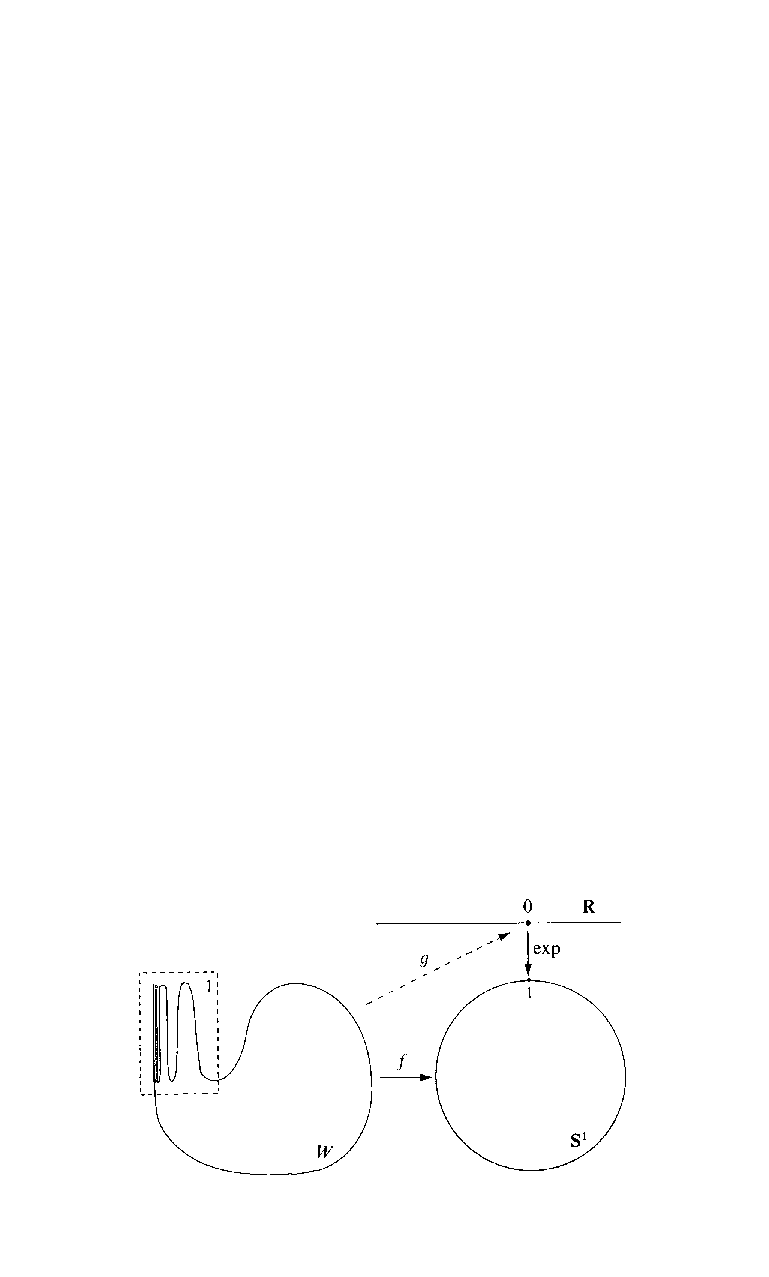
\includegraphics[width=0.7\textwidth]{figures/discont_lift.pdf}
    \caption{The map $f$ here collapses the entire ``$\sin 1/x$'' part of the space on the left into the basepoint $1$ on the circle. If a lifting map $g$ into the real line existed, then the vertical part of the ``$\sin 1/x$'' curve would have to be mapped to $0$, whereas the wiggly part would map to $1$ under $g$, making it discontinuous. From \cite[Fig.~III-6]{Bredon}.}
    \label{fig:discont_lift}
\end{figure}

\begin{thm}[Lifting Theorem]\index{Theorem!Lifting}\label{Lifting Theorem}
    Let $\pi:E\to M$ be a covering map with $\pi (p_0)=x_0$. Assume that $W$ is path-connected and locally path-connected and that $f:W\to M$ is a map with $f(w_0)=x_0$. Then a pointed map $\wt f:(W,w_0)\to (M,x_0)$ such that $\pi\circ\wt{f}=f$ exists iff $f_\ast (\pi_1(W,w_0))\subset \pi_\ast (\pi_1(E,p_0))$. Moreover, $\wt f$ is unique.
\end{thm}
\begin{proof}
    Let us construct $\wt f$ explicitly. Given $w\in W$, let $\lambda:I\to W$ be a path from $w_0$ to $w$. Then $f\circ \lambda$ is a path in $M$. Lift this to a path $\wt\lambda:(I,0)\to (E,x_0)$ and let $\wt{f}(w)=\wt{\lambda}(1)$. Then $\pi\circ \wt{f}(w)=\pi(\wt{\lambda}(1))=f(\lambda(1))=f(w)$.

    To see that $\wt{f}$ is well defined, suppose $\lambda'$ is another path in $W$ from $w_0$ to $w$ and let $\eta=(\lambda ')^{-1}$ be the reverse path from $w$ to $w_0$. Then $\lambda\bullet \eta$ is a loop based at $w_0$, and $(f\circ \lambda)\bullet (f\circ\eta)$ is a loop in $M$ based at $x_0$. Since 
    \[[f\circ\lambda \bullet f\circ\eta]=f_\ast([\lambda\bullet\eta]\in \im(f_\ast)\subset \im(\pi_\ast),\]
    $f\circ\lambda\bullet f\circ\eta$ lifts to a loop in $E$ based at $p_0$. The reverse of the portion of this lifting corresponding to $\eta$ then is a lifting $\wt{\lambda}'$ of $\lambda '$ and $\wt{\lambda}'(1)=\wt{\lambda}(1)$, as required.

    Next, we have to show that $\wt{f}$ is continuous. Let $w\in W$  and put $x=f(w)$. Let $U\subset <$ be an elementary neighborhood of $x$, and by local path-connectedness of $W$ we can let $V$ be a path-connected neighborhood of $w$ such that $f(V)\subset U$. For any point $w'\in V$ we can construct a path from $w_0$ to $w'$ by concatenating a given path $\lambda$ to $w$ with a path $\sigma$ in $V$ from $w$ to $w'$. Since $f(V)$ is contained in an elementary set, the lifting of $f\circ \sigma$ is simply $f\circ\sigma$ composed with the local inverse of $\pi$ that takes $U$ to the component of $\pi^{-1}(U)$ that contains $\wt{f}(w)$. This same component is used for all $w'\in V$ and it follows that $\wt{f}$ is continuous at $w$.

    The converse direction of the theorem follows immediately from $f_\ast=\pi_\ast\circ \wt{f}_\ast$.
\end{proof}
\begin{rem}
    Unlike in the homotopy lifting property (Theorem~\ref{homotopy lifting property}), the condition of local path connectedness for $W$ cannot be dropped here. See an example in Figure~\ref{fig:discont_lift}.
\end{rem}

\begin{cor}[{{\cite[Cor.~4.2]{Bredon}}}]\label{cor 4.2 Bredon}
    Under the conditions of the Lifting Theorem~\ref{Lifting Theorem}, if $W$ is also simply connected, then the lifting $\wt{f}$ always exists and is unique given a basepoint $p_0\in E$.
\end{cor}

\begin{cor}\label{cor homotopy groups of coverings}
    Given a covering space $E\overset{\pi}{\to}M$, there is a natural isomorphism of higher homotopy groups
    \[\pi_n(E,p_0)\cong \pi_n(M,x_0),\; n\geq 2.\]
\end{cor}
\begin{proof}
    Injectivity follows from the uniqueness of the liftings of maps $\bbS^n\to M$ into $E$. Surjectivity follows from the Lifting Theorem~\ref{Lifting Theorem} combined with the fact that $\pi_1(\bbS^n)$ is trivial for $n\geq 2$ (Corollary~\ref{cor pi_1(S^n)=0}).
\end{proof}

\begin{cor}\label{cor: homotopy groups of circle}
    $\pi_n(\bbS^1)=1$ for $n>1$.
\end{cor}
\begin{proof}
    Any map $f:\bbS^n\to \bbS^1$ lifts to $\wt{f}:\bbS^n\to \bbR $ by Corollary~\ref{cor 4.2 Bredon}. But $\wt f$ is homotopically trivial since $\bbR $ is contractible, so $f=\pi\circ\wt{f}$ is also homotopically trivial.
\end{proof}


\section{Morphisms of covering spaces}


\begin{defn}[Category of covering spaces]
The category $\mathsf{Cov}_M$ of covering spaces of a given base $M$ (say, topological covering spaces) consists of all covering spaces of $M$. The morphisms between two covering spaces $\pi$ and $\pi'$ are morphisms $f:E\to E'$ that ``map fibers to fibers'', i.e., $\pi'\circ f=\pi$, or equivalently if the following triangle commutes:
\[
\begin{tikzcd}[every matrix/.append style={name=m},   
execute at end picture={\draw [<-] ([xshift=0mm,yshift=-2mm]m-2-2.north) arc[start angle=-90,delta angle=-270,radius=0.25cm];}]
   E \arrow[rr,"f"]\arrow[ddr,swap,"\pi"]& & E'\arrow[ddl,"\pi'"]\\
   & \, & \\
   & M & \\
\end{tikzcd}
\]
\end{defn}


\begin{lem}[{{\cite[Lem.~4.4]{Bredon}}}]\label{lem 4.4 Bredon}
    Let $W$ be connected and $E$ be Hausdorff. Let $\pi:E\to M$ be a covering map and $f:W\to M$ a map. Let $\wt{f}_1,\wt{f}_2$ be two liftings of $f$ into $E$. If $\wt{f}_1(w)=\wt{f}_2(w)$ for some point $w\in W$, then $\wt{f}_1\equiv \wt{f}_2$.
\end{lem}
\begin{proof}
    Let $\wt{f}_1(w)=\wt{f}_2(w)=p$. Let $U$ be an elementary open neighborhood of $f(w)$ in $M$. Let $V$ be the component of $\pi^{-1}(U)$ containing $p$. Then $A=\wt{f}_1^{-1}(V)\cap\wt{f}_2^{-1}(V) $ is an open set in $W$ and for $a\in A$ we have $\wt{f}_1(a)=\wt{f}_2(a)$ since the homeomorphism $\pi:V\to U$ maps them both to $f(a)$. This shows that the set $\{w\in W\mid \wt{f}_1(w)=\wt{f}_2(w)\}$ is open. But this set is also closed since it is the inverse image of the diagonal under the map $\wt{f}_1\times \wt{f}_2:W\to E\times E$, and the diagonal is closed since $E$ is Hausdorff. Since $W$ is connected, this set is either empty or all of $W$.
\end{proof}
\begin{cor}[{{\cite[Cor.~4.5]{Bredon}}}]\label{cor 4.5 Bredon}
    Let $\pi_i:E_i\to M$, $i=1,2$, be covering maps such that $E_1$ is simply connected, and let $p_i\in E_i$ be such that $\pi_1(p_1)=\pi_2(p_2)$. Then there is a unique morphism of covering spaces $f:E_1\to E_2$ such that $f(p_1)=p_2$. Moreover, $f$ is a covering map.
\end{cor}
\begin{proof}
    By the Lifting Theorem~\ref{Lifting Theorem}, since $\pi_1(E_1,p_1)=1$, there is a lifting of $\pi_1\to E_1\to M$ to a map $f:E^1\to E^2$ such that $\pi_2\circ f=\pi_1$. It is unique by Lemma~\ref{lem 4.4 Bredon}.  It is an easy exercise to show that $f$ is a covering map.
\end{proof}
\begin{cor}[{{\cite[Cor.~4.6]{Bredon}}}]\label{cor 4.6 Bredon}
    If in Corollary~\ref{cor 4.5 Bredon} both $E_1$ and $E_2$ are simply connected, then the unique map $f$ is a homeomorphism.
\end{cor}
\begin{proof}
    By Corollary~\ref{cor 4.5 Bredon}, in addition to $f$ there is also an analogous map $k:E_2\to E_1$. Then $k\circ f:E_1\to E_1$ covers the identity map at $p_1$. By Lemma~\ref{lem 4.4 Bredon}, it must equal the identity everywhere. Similarly $g\circ k=\mathrm{id}_{E_2}$, hence $k=f^{-1}$.
\end{proof}

This implies that all simply connected covering spaces of a given base space $M$ are isomorphic in the category $\mathsf{Cov}_{\bullet M}$. Such covering spaces are called \emph{universal}, and are guaranteed to exist under the following mild restriction.

\begin{defn}[Locally relatively simply connected space]
    A space $X$ is locally relatively simply connected (or semilocally simply connected) if each point has a neighborhood $U$ such that all loops inside of $U$ are homotopically trivial in $X$ (i.e., for any $u\in U$ the homomorphism $\pi_1(U,u)\to \pi_1(X,u)$ is trivial).
\end{defn}

One can show that the existence of a simply connected covering space is equivalent to $M$ being locally relatively simply connected (see~\cite[Theorem~8.4]{Bredon}). Since we are mostly interested in manifolds, we will only prove the existence. Let us only work with connected, locally simply connected spaces (in particular, connected manifolds).

\begin{figure}[tp]
    \centering
    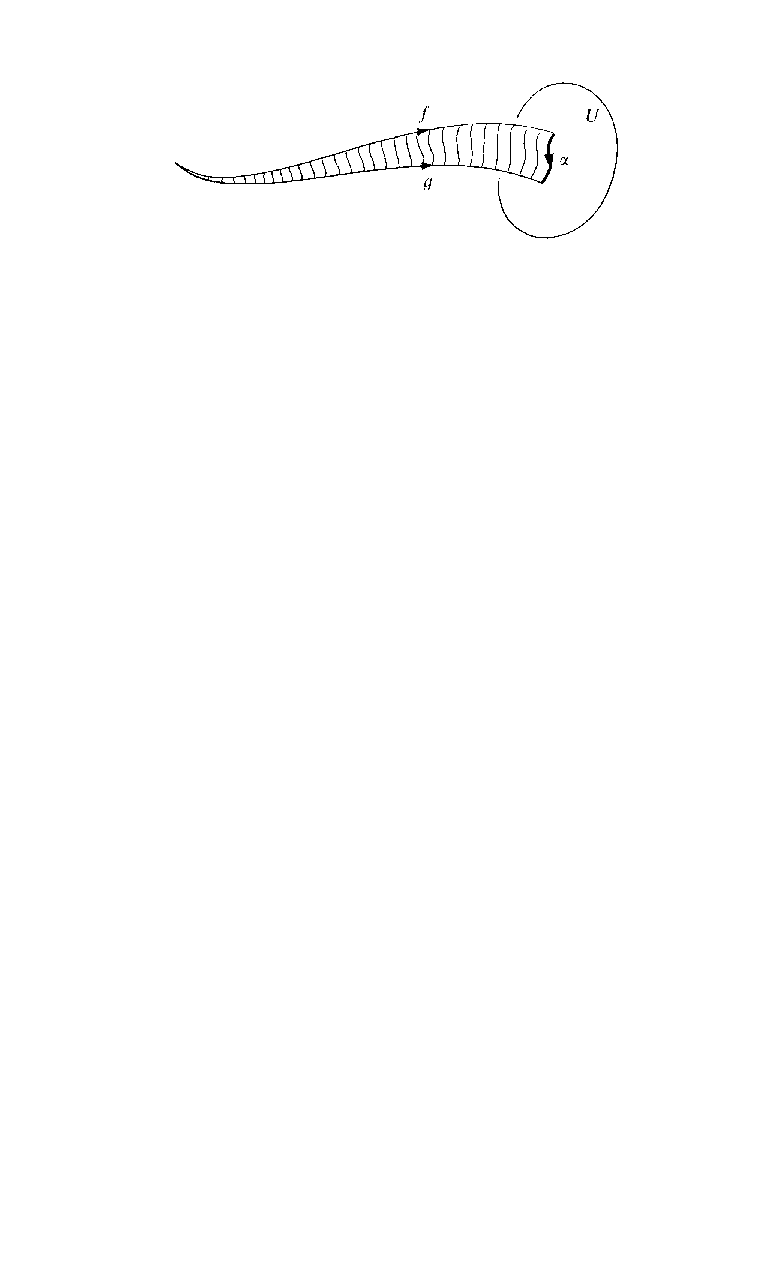
\includegraphics[width=0.5\textwidth]{figures/uni_open_set.pdf}
    \caption{Topology of the universal cover.\label{fig univ cover}}
\end{figure}

\begin{thm}[Universal cover {{\cite[Thm.~11.43]{LeeTop}}}, {{\cite[Thm.~8.4]{Bredon}}}]\index{Universal cover}
    For a given base $M$ that is a connected and \emph{locally relatively simply connected} Hausdorff space, there is a unique (up to homeomorphism) topological covering space $E\overset{\pi}{\to}M$ whose total space $E$ is simply connected. This covering space is denoted by $\wt M$ and is called the \emph{universal cover} of $M$.\index{Universal cover}
\end{thm}
\begin{proof}
    For the full proof see the references in the title. The basic idea is to explicitly construct $\wt M$ as the space of endpoints of all possible paths in $M$ based at a fixed point $m\in M$. Two paths are equivalent if their endpoints coincide and they are homotopic with fixed endpoints. The topology on this set of paths is introduced by considering sets of homotopic paths with endpoints belonging to an open set in $M$ (and the homotopies fix the starting point but can move the endpoint within the open set, see Figure~\ref{fig univ cover}). The projection $\pi$ maps a path to its endpoint. It is not difficult to check that this is indeed a topological covering map and the total space is simply connected. Uniqueness will follow from the universal property described below.
\end{proof}
\begin{rem}
    By examining the details of the proof one can notice that local simply-connectedness is not actually required, and semilocal simply-connectedness is sufficient. The converse direction is clear: if a loop is in an evenly covered subspace of $M$ then it lifts to $E$, and if $E$ is simply connected, the loop must be trivial in $E$. But then the composition of its homotopy to a constant loop with the covering map $\pi$ shows that the original loop in $M$ must be trivial. Thus we have shown that a connected and locally path-connected $M$ has a universal covering space iff it is locally relatively simply connected.
\end{rem}
\begin{example}
    The Hawaiian earring (Example~\ref{hawaiian earring}), as well as the infinite-dimensional torus $\bbT^\infty=\prod_{i=1}^\infty \bbS^1$, are not locally relatively simply connected, and thus don't have universal coverings.
\end{example}

\begin{thm}[{{\cite[Prop.~4.40]{Lee}}}]
Let $E\overset{\pi}{\to}M$ be a topological covering map and fix a smooth structure on $M$. Then $E$ is a topological manifold that supports a unique smooth structure such that $\pi$ is a smooth covering map with $\pi^{-1}(\partial M)=\partial E$.
\end{thm}

This theorem essentially means that in order to classify smooth covering spaces above a smooth base manifold, it suffices to only classify the topological covering spaces, and they are in one-to-one correspondence with the smooth ones. In other words, the theory of covering spaces is an intrinsically topological theory that doesn't gain or lose anything from imposing smooth structures.

\begin{cor}
For a connected smooth manifold $M$, there exists a unique simply connected smooth covering space called the universal covering manifold of $M$.
\end{cor}
From now on we won't really distinguish between smooth and topological covering spaces, although we only care about the smooth case.

Corollaries~\ref{cor 4.5 Bredon} and \ref{cor 4.6 Bredon} can now be restated in terms of morphisms:
\begin{cor}[Universality of the universal cover]\index{Universal property!of universal covers}
    \;
    \begin{enumerate}
       \item Any morphism of covering spaces is itself a covering map;
        \item If $M$ is a topological manifold (or any space that has a universal covering space), then $\wt{M}$ is the initial object in the category $\mathsf{Cov}_{\bullet M}$ of pointed covering spaces of $M$ (i.e., objects are $E\overset\pi\to M$ with a basepoint $p_0\in E$ and morphisms must respect the basepoints).
    \end{enumerate}
\end{cor}

In the category of non-pointed covering spaces, the universal cover is not an initial object, but the arrows coming out of it are unique up to automorphisms of the two covering spaces at the ends of the arrow. We now describe the sets of such automorphisms.

\section{Deck transformations}

\begin{defn}[Group action]
    An (right/left) action of a group $G$ on a set (or a space, a manifold) $X$ is a map $\Phi: G\times X\to X$, with its partial maps denoted by $\Phi_g=\Phi (g,\_):X\to X$ and $\Phi_x=\Phi(\_,x):G\to X$, such that $\Phi_e=\mathrm{id}_X$ and one of the following:
    \begin{align}
        \text{left action}:&& \Phi_g\circ \Phi_h&=\Phi_{gh},\\
        \text{right action}:&& \Phi_g\circ \Phi_h&=\Phi_{hg}.
    \end{align}
    In other words, right actions are the same thing as left actions on the opposite group $G^{\mathrm{op}}$. For this reason right actions are usually written as $x\cdot g=\Phi_g(x)$ and left actions as $g\cdot x=\Phi_g(x)$. The sets $G(x)=\Phi_x(G)$ are called \emph{orbits}.
\end{defn}
In the topological and smooth categories one usually considers continuous or smooth group actions, provided $G$ is a Lie group, but we will delay that discussion until \S\ref{sec: Lie group actions}. For now $G$ will always be a discrete group (i.e., a group with discrete topology), so any condition of continuity or smoothness on the action is simply a condition on each $\Phi_g$ individually.

\begin{defn}[$G$-equivariant maps]\index{Equivariant maps}\index{$G$-Set}
    The category of sets (spaces, manifolds) carrying a (left) action of $G$ is called $G\mathsf{-Set}$. Morphisms in this category are maps $f:X\to Y$ such that for all $g\in G$, $f(g\cdot x)=g\cdot f(x)$. These maps are called $G$-equivariant. Similarly, $G\mathsf{-Set}_\bullet$ consists of pointed sets with equivariant maps that respect basepoints. 
\end{defn}
\begin{defn}[Stabilizer]\index{Stabilizer}
    Given a group $G$ acting on a set $X$, and a point $x\in X$, the stabilizer of $x$ is defined as the subgroup $G_x=\{g\in G\mid \Phi(g,x)=x\}$.
\end{defn}
\begin{defn}[Transitive action]
    An action $\Phi$ is called transitive if it has only one orbit, i.e., for each pair $x,y\in X$ there is an $g\in G$ such that $\Phi(g,x)=y$.
\end{defn}
\begin{defn}[Simply transitive action]
    An action $\Phi$ is called simply transitive if for each pair $x,y\in X$ there is a \emph{unique} element $g\in G$ such that $\Phi(g,x)=y$.
\end{defn}
\begin{defn}[Faithful action]
    An action $\Phi$ is called faithful if no nontrivial elements of $G$ act trivially: $\Phi_g=\mathrm{id}_X \Leftrightarrow g=e$.
\end{defn}
\begin{defn}[Free action]
    An action $\Phi$ is called free if no nontrivial elements of $G$ have any fixed points: $\exists\,x\in X: \Phi(g,x)=x\Leftrightarrow g=e$. 
\end{defn}
\begin{prop}
    An action is simply transitive iff it is free and transitive.
\end{prop}
\begin{proof}
    Assume a left action for simplicity. For the necessary condition, we only need to show freeness. If $\Phi_g=\mathrm{id}_X$, then $g\cdot x=x=e\cdot x$, therefore by simple transitivity $g=e$.

    For the converse, assume there are two elements such that $g_1\cdot x=g_2\cdot x=y$. Then $g_2^{-1}g_1\cdot x=x$, which means $g_2^{-1}g_1=e$ by freeness.
\end{proof}

Throughout this section let $E\overset{\pi}{\to}M$ be a covering space with a fixed point $x_0\in M$. For simplicity we also denote
\[G=\pi_1(M,x_0),\quad \quad F=\pi^{-1}(x_0).\]
The discrete set $F$ is called the \emph{fiber} of $\pi$ over $x_0$. We are going to describe an action of the group $G$ on $F$ as a group of permutations. 

Let $p\in F$ and let $g\in G$ be an element represented by a loop $\gamma :I\to M$. Lift it to get a map $\wt{\gamma}$ in $E$ with $\wt{\gamma}(0)=p$. Then define
\[\Phi(g,p)=p\cdot g =\tilde{\gamma}(1) \in F.\]
By Corollary~\ref{cor 3.5 Bredon} this does not depend on the choice of $\gamma$ and thus is a well-defined map $\Phi:F\times G\to F$. Now we can check some properties of this function:
\begin{enumerate}
    \item $x\cdot e=x$.
    \item $(x\cdot g)\cdot h=x\cdot (gh)$, i.e., it is a right action (because the product of two loops $gh$ corresponds to the application of $\Phi_g$ and then $\Phi_h$).
    \item $E$ is connected iff this action is transitive (i.e., there is only one orbit, $p\cdot G=F$). To see this, pick a path in $E$ from $p_0$ to another $p\in F$. This projects onto a loop $\gamma$ in $M$ and $g=[\gamma]$ provides the required element: $p_0\cdot p=p$. Conversely, if $E$ is not connected, the action is obviously not transitive.
    \item The stabilizer of a point is $G_{p_0}=\{g\in G\mid p_0\cdot g=p_0\}$. Then 
    \[
        \boxed{G_{p_0}=\im \pi_\ast=\pi_\ast(\pi_1(E,p_0))}\label{stabilizer}
    \]
    where $\pi_\ast:\pi_1(E,p_0)\to \pi_1(M,x_0)=G$ is the homomorphism induced by $\pi$. This is true because $g\in G_{x_0}$ iff $g=[\gamma]$ and $\gamma$ lifts to a loop at $p_0$, i.e., iff $g\in \im p_\ast$.
    \item Assuming $E$ is connected, the map $\phi: \ _{G_{p_0}}\bslash^{G}\to F$ taking the right coset $G_{x_0}g$ to $p_0\cdot (G_{p_0}g)=p_0\cdot g$ is a bijection.
\end{enumerate}
Obviously any covering space decomposes into a disjoint union of connected components, and the action of $\pi_1(M)$ is transitive on the fiber of each component separately. In what follows, we generally assume that $E$ is connected. In summary, we have the following theorem.
\begin{thm}
    Given a connected covering space $\pi:E\to M$, there is a one-to-one correspondence between the set $_{\pi_\ast(\pi_1(E,p_0))}\bslash^{\pi_1(M,x_0)}$ of right cosets, and the fiber $\pi^{-1}(x_0)$. (Note that $\pi_\ast(\pi_1(E,p_0))\cong \pi_1(E,p_0)$ since $\pi_\ast$ is a monomorphism by Corollary~\ref{cor 3.7 Bredon}.)
\end{thm}
\begin{cor}
    The number of sheets of a connected covering space equals the index (number of left or right cosets) of $G_{p_0}=\pi_\ast(\pi_1(E,p_0))$ in $G=\pi_1(M,x_0)$.
\end{cor}
\begin{cor}
    If $\wt\pi:\wt M\to M$ is a universal covering map (i.e., $\wt M$ is simply connected), then the number of sheets equals the order (cardinality) of the group $\pi_1(M,p_0)$.
\end{cor}

\begin{example}[Fundamental groups of real projective spaces]
    Since $\bbS^n$ is simply connected for $n>1$ and $\bbS^n$ is a double covering of the real projective space $\RP^n$, it follows that $\pi_1(\RP^n)\cong \bbZ_2$.
\end{example}

\begin{defn}[Deck transformations]\index{Deck transformations}
    For a covering space $E\overset{\pi}{\to}{M}$, consider the group $\Aut(\pi)$ of automorphisms of this covering space in the category $\mathsf{Cov}_M$ (also called \emph{deck transformations}). Its elements are homeomorphisms of $E$ that cover the identity map on $M$. For a given elementary open set $U\subset M$, they permute the connected components $U_i$ of the preimage $\pi^{-1}(U)$. In other words, the group $\mathrm{Aut}(\pi)$ acts on $E$ via morphisms of covering spaces.
\end{defn}

\begin{prop}[{{\cite[Prop.~6.2]{Bredon}}}]\label{prop 6.2 Bredon}
    If $a\in \Aut(\pi)$ and $g\in\pi_1(M,p_0)$ and $x\in \pi^{-1}(x_0)$ then $a(x)\cdot g=a(x\cdot g)$. In other words, deck transformations are equivariant with respect to the action of $\pi_1(M,x_0)$.
\end{prop}
\begin{proof}
    Let $\gamma$ be a loop at $x_0$ representing $g$ and lift it to a path $\wt\gamma$ starting at $p$. Then $\wt\gamma(1)=p\cdot g$ by definition. Look at the path $a\circ \wt{\gamma}$. It is a lifting of $\gamma$ and starts at $a(p)$. Thus is ends at $a(p)\cdot g$ by definition of the latter. But it also ends at $a(\wt\gamma(1))$, which is $a(p\cdot g)$.
\end{proof}

This proof actually shows that not only automorphisms are $G$-equivariant, but all morphisms in the category $\mathsf{Cov}_M$ are. This means that the action of $\pi_1(M)$ that we've constructed is \emph{natural}. These results can be summarized by the following theorem.
\begin{thm}[Monodromy Action]\index{Monodromy (covering spaces)}
For any covering space $E\overset{\pi}\to M$, 
\begin{enumerate}
    \item there is a natural homomorphism $\pi_1(M)\to \Aut(\pi)$ called the \emph{monodromy action};
    \item $\Aut(\wt \pi)\cong\pi_1(M)$, where $\wt\pi$ is the universal cover.
\end{enumerate}
\end{thm}

\begin{defn}[Normalizer]\index{Normalizer of a subgroup}
For a subset (not necessarily a subgroup) $H\subset G$ of a group $G$, its normalizer is 
\[\rmN_G(H)=\{n\in G\mid nH=Hn\}.\]
A subgroup $H$ is normal in $G$ iff $\rmN_G(H)=G$. Otherwise, $\rmN_G(H)$ is the largest subgroup of $G$ such that $H$ is a normal subgroup of $\rmN_G(H)$.
\end{defn}
\begin{rem}
    If $H$ is a subgroup, then $H\subset \rmN_H(H)$. Moreover, $\rmN_G(g^{-1}Hg)=g^{-1}\rmN_G(H)g$, so the normalizers of conjugate subsets are conjugate.
\end{rem}

The following lemma is the analog of the ``change of coordinates'' formulas in linear algebra: mapping the coordinates of vectors to a new basis is equivalent to conjugating the matrices representing linear operators.
\begin{lem} For any group $G$ acting on a set $X$ from the right,
\[\boxed{G_{p_0\cdot g}=g^{-1}G_{p_0}g.}\label{conjugate stabilizers}\]
Similarly, for left actions, $G_{g\cdot p_0}=gG_{p_0}g^{-1}$.
\end{lem}
\begin{proof}
    \[
        G_{p_0\cdot g}=\{h\mid (p_0\cdot g)\cdot h=p_0\cdot g\}=\{h\mid p_0\cdot ghg^{-1}=p_0\}=\{h\mid ghg^{-1}\in G_{p_0}\},
    \]
\end{proof}

The most important question in the study of deck transformations is: given two points in the fiber, when does there exist a deck transformation mapping one to the other? This is answered in the following theorem.
\begin{thm}[{{\cite[Thm.~6.3]{Bredon}}}]\label{thm 6.3 Bredon}
    Provided $E$ is connected, let $p,p_0\in F=\pi^{-1}(x_0)$, $G=\pi_1(M,x_0)$ and $G_{q}=\pi_\ast(\pi_1(E,q))$ for any $q\in E$. Then \gls{tfae}:
    \begin{enumerate}[label=(\arabic*)]
        \item $\exists\, a\in \mathrm{Aut}(\pi)$ such that $a(p_0)=p$.
        \item $\exists\, g\in \rmN_G(G_{p_0})$ such that $p_0\cdot g=p$.
        \item $G_{p_0}=G_p$.
    \end{enumerate}
\end{thm}
\begin{proof}
    Recall that $G_{p_0}=\pi_\ast(\pi_1(E,p_0))$ and $G_{p}=\pi_\ast(\pi_1(E,p))$. By the Lifting Theorem~\ref{Lifting Theorem} a map $a$ covering the identity and taking $p_0$ to $p$ exists iff $\pi_\ast(\pi_1(E,p_0))\subset \pi_\ast(\pi_1(E,p))$. Similarly, a map $a'$ covering the identity and mapping $p$ to $p_0$ exists iff the opposite inclusion holds. If both exist then $a\circ a'$ covers the identity and has a point in common with the identity, therefore $a\circ a'=\mathrm{id}_E$ by Lemma~\ref{lem 4.4 Bredon}. This proves the equivalence $(1)\Leftrightarrow (3)$.

    Now we can prove $(2)\implies(3)$: if $p=p_0\cdot g$ and $g\in \rmN_G(G_{p_0})$ then $G_p=G_{p_0\cdot g}=g^{-1}G_{p_0}g=G_{p_0}$ as claimed.

    For $(3)\implies (2)$, suppose $G_{p_0}=G_p$ and $p=p_0\cdot g$ (such a $g$ exists since $G$ acts transitively on $F$). Then $G_{p_0}=G_p=G_{p_0\cdot g}=g^{-1}G_{p_0}g$, so $g\in \rmN_G(G_{p_0})$.
\end{proof}
From $(2)\Leftrightarrow(1)$ and the last part of the proof we have the following Corollary.
\begin{cor}[{{\cite[Cor.~6.4]{Bredon}}}]\label{cor 6.4 Bredon}
    For a connected covering space, the subgroup $G_{p_0}=\pi_\ast(\pi_1(E,p_0))$ is normal in $G=\pi_1(M,x_0)$ iff the action of $\mathrm{Aut}(\pi)$ is (simply) transitive on $F=\pi^{-1}(x_0)$.
\end{cor}
\begin{cor}[{{\cite[Cor.~6.5]{Bredon}}}]\label{cor 6.5 Bredon}
    In a connected covering space, if $p$ ranges over the fiber $F$ then $G_p$ ranges over all conjugates of $G_{p_0}=\pi_\ast(\pi_1(E,p_0))$.
\end{cor}
\begin{proof}
    This is a consequence of (\ref{conjugate stabilizers}).
\end{proof}

\begin{rem}
    It is worth providing some intuition for normalizers. If two points in a $G$-set belong to the same orbit, i.e., they can be mapped into each other by some elements of $G$, then their stabilizers are obviously conjugate subgroups of $G$.

    By definition, conjugation doesn't change a normal subgroup (as a set, not pointwise). Therefore if a stabilizer of a point is normal, then all other points in that orbit have the same exact stabilizer. In particular, this means that the only elements of the group which actually move the points in the orbit are the cosets of the normal stabilizer. Moreover, if you have two group elements from the same coset of this normal stabilizer, then they act on the orbit \emph{in the exact same manner}.
\end{rem}

\begin{defn}[Regular covering map]
    A covering map $\pi$ is called regular if $\mathrm{Aut}(\pi)$ is transitive on the fiber. In the case of a connected total space this is equivalent to $G_{p_0}=\pi_\ast(\pi_1(E,p_0))$ being normal in $\pi_1(M,x_0)$.
\end{defn}

In other words, normal subgroups of $\pi_1(M,x_0)$ correspond to regular connected covering spaces of $M$. A regular covering space is one whose fundamental group ``looks the same'' in terms of the generators of $\pi_1(M,x_0)$ regardless of the choice of the basepoint $p_0$ in the fiber. Such covering spaces have an inherent ``symmetry'' given by the quotient group $G/G_{p_0}$ (which exists because $G_{p_0}$ is normal). Obviously, any regular covering space that is not connected is a disjoint union of isomorphic connected regular covering spaces. Hence, it suffices to study only the connected ones. For an example of a connected non-regular covering space, see Figure~\ref{fig:threefold-cover}.

\begin{figure}
    \centering
    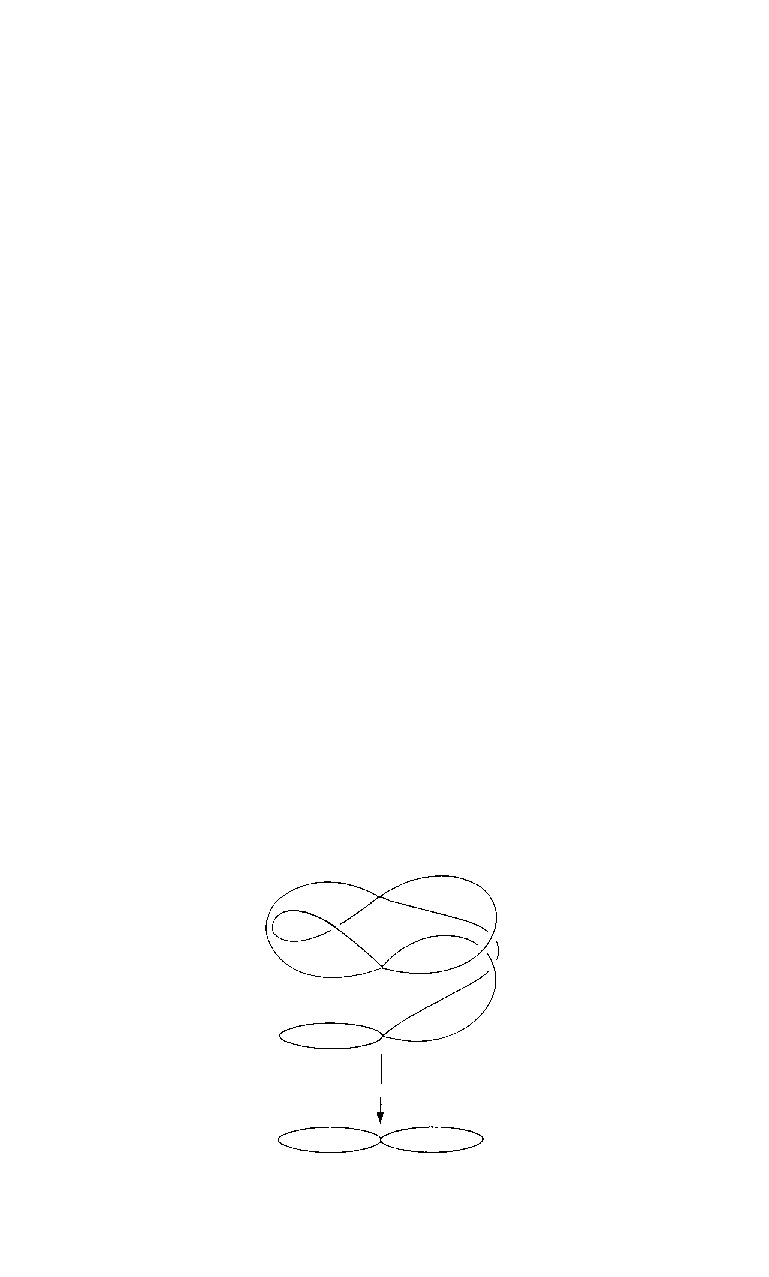
\includegraphics[width=0.4\textwidth]{figures/threefold_cover.pdf}
    \caption{This threefold cover of the figure eight space is not regular. Indeed, its group of automorphisms is trivial.}
    \label{fig:threefold-cover}
\end{figure}

\begin{rem}
    These ideas comprise the powerful \emph{Reidemeister-Schreier method} for finding presentations of subgroups $H\leq G$ given a presentation of $G$. Namely, one constructs a base space whose fundamental group is $G$, then finds a covering space corresponding to $H$ and computes its fundamental group.
\end{rem}

\begin{defn}
    Define the map $\Theta:\rmN_G(G_{p_0})\to \mathrm{Aut}(\pi)$ by $\Theta(g)=a_g$ where $a_g$ is the unique deck transformation such that $a_g(p_0)=p_0\cdot g$.
\end{defn}
\begin{thm}[Classification of Deck Transformations {{\cite[Thm.~6.8]{Bredon}}}]\label{thm 6.8 Bredon}
    $\ker \Theta=G_{p_0}$, and consequently,
    \[\mathrm{Aut}(\pi)\cong \rmN_G(G_{p_0})\slash G_{p_0}.\]
\end{thm}
\begin{proof}
    First, 
    \[a_h(a_g(p_0))=a_h(p_0\cdot g)=a_h(p_0)\cdot g=(p_0\cdot h)\cdot g=p_0\cdot (hg)=a_{hg}(p_0).\]
    This proves that $\Theta$ is a homomorphism. Next note that if $a\in \mathrm{Aut}(\pi)$ then there is an $g\in \rmN_G(G_{p_0})$ such that $a(p_0)=p_0\cdot g=a_g(p_0)$. Therefore $a=a_g$, which shows the surjectivity of $\Theta$.

    Finally we compute the kernel of $\Theta$. The result follows from the chain of equivalences
    \[a_g=\mathrm{id}_E \Leftrightarrow p_0\cdot g=p_0\Leftrightarrow g\in G_{p_0}.\]
\end{proof}
\begin{cor}
    If the covering map $E\overset{\pi}{\to} M$ is regular, then 
    \[\mathrm{Aut}(\pi)\cong G/G_{p_0}\]
\end{cor}
\begin{cor}
    If $\wt{M}\overset{\wt\pi}{\to} M$ is a universal covering map, then
    \[\mathrm{Aut}(\wt\pi)\cong G=\pi_1(M,x_0).\]
\end{cor}





\section{Classification of covering spaces}

Our examination of connected covering spaces allows us to easily prove the following classification of connected covering spaces in terms of subgroups of the fundamental group of the base.

\begin{thm}[Classification of coverings I]
    Let $M$ be path-connected and semilocally simply connected so that it has a universal covering space $\wt{M}$. Then the following \emph{Galois correspondence} holds:
\begin{enumerate}
	\item The isomorphism classes of connected pointed covering spaces of $M$ are in one-to-one correspondence with subgroups of $G=\pi_1(M, x_0)$. 
	\item The isomorphism classes of connected covering spaces of $M$ without basepoints are in one-to-one correspondence with the conjugacy classes of subgroups of $G=\pi_1(M, x_0)$.
    % sets $F$ (finite or countable) with an action of the group $\pi_1(M)$ (a group action on $F$ is an element of $\Hom(\pi_1(M),G)$, where $G$ is the full permutation group of the points of $F$).
\end{enumerate}
The correspondence is given by $E\leftrightarrow \pi_\ast(\pi_1(E,p_0))=G_{p_0}$ where $\pi$ is the covering map.
\end{thm}
\begin{proof}
    The second statement follows from the first combined with Corollary~\ref{cor 6.5 Bredon}. It remains to show that the map taking a covering map with a basepoint, $\pi:(E,p_0)\to (M,x_0)$, into the subgroup $\pi_\ast(\pi_1(E,p_0))$ of $\pi_1(M,x_0)$ is a bijection. It is an injection by the Lifting Theorem~\ref{Lifting Theorem}. 
    
    To see that it is a surjection, suppose that $H\subset \pi_1(M,x_0)=G$ is a subgroup. Since $\wt{M}$ is simply connected, Theorem~\ref{thm 6.8 Bredon} gives the isomorphism $\Theta:G\to \mathrm{Aut}(\pi)$, where $\Theta(g)=a_g$. Under this map, $H$ is mapped to a subgroup $A_H\leq \mathrm{Aut}(\pi)$. Put $E=\wt{M}/A_H$ which projects to $M$ canonically. Let $p_0$ be the image of the basepoint $\wt{p}_0\in\wt{M}$. We wish to identify $\pi_\ast(\pi_1(E,p_0))$. Let $\gamma$ be a loop in $X$ at $p_0$. Lifting this to $\wt{M}$ at $\wt{p}_0$ gives the same path as a lifting of the projection of $\gamma$ to a loop at $x_0$ in $M$. Thus the lifting ends at $a_g(\wt{p}_0)$, where $g\in\pi_1(M,x_0)$ is the homotopy class of the projection of $\gamma$ to $M$. But for $\gamma$ to be a loop in $E=\wt{M}/A_H$, we must have that $\wt{p}_0$ and $a_g(\wt{p}_0)$ are in the same orbit of $A_H$. This is true iff $a_g\in A_H$, and this holds iff $g\in H$. But $g$ is an arbitrary element of $\pi_\ast(\pi_1(E,p_0))$. Thus $H=\pi_\ast(\pi_1(E,p_0))$.
\end{proof}


Now we restate the classification theorem as it was described in Example~\ref{covering category thm}. We consider all, not only connected, coverings. 

Given an action of a group $G$ on a space $X$, the space $X$ decomposes into a disjoint union of orbits of $G$. Let us assume a discrete topology on $G$, in which case a continuous/smooth action is simply one for which the maps $\Phi_g:X\to X$ are continuous/smooth for all $g$. The set of all orbits is denoted by $X\slash G$ and, if imbued with the quotient topology descended from $X$, is called the \emph{orbit space}. Note that the canonical projection $p:X\to X\slash G$ that takes a point to its orbit is open because for an open $U\subset X$, $p^{-1}(p(U))=\bigcup_g (g\cdot U)$, which is a union of open sets.

Every covering map of $M$ gives rise to an action of $G=\pi_1(M,x_0)$ on the fiber $F=F_{x_0}$. Under this action $F$ decomposes into a disjoint union of orbits $F_j$, each of them associated with a conjugacy class of stabilizer subgroups $H_j<G$. This determines a functor from the category $\mathsf{Cov}_M$ of coverings of $M$ to the category $G\mathsf{-Set}$ of sets with a (left) action of $G=\pi_1(M,x_0)$. If $F$ is a $G$-set with a transitive action of $G$, then the stabilizers of any two of its points are conjugate subgroups of $G$. Choosing $p_0\in F$ and denoting $H=G_{p_0}$, we have that $F$ is isomorphic to the set of cosets $G\slash H$, also called a \emph{homogeneous set}. From such a $G$-set $F$ we can easily reconstruct a connected covering space $\pi$ by taking the universal covering space $\wt{M}$ and letting $\pi:\wt{M}\to \wt{M}\slash H$ be the orbit map of the action of $H$ on $\wt{M}$. If $F$ is not homogeneous, then it is a disjoint union of homogeneous sets (orbits), and the corresponding covering space is a disjoint union of the corresponding connected ones. This provides a functor in the opposite direction. It is easy to check that these two functors are each other's quasi-inverses. We thus have the second version of the theorem.

\begin{thm}[Classification of coverings II {{\cite[Thm.~3.3.2]{tomDieck}}}]\label{covering spaces category equivalence thm}
    If $M$ admits a universal covering space, then the category $\mathsf{Cov}_M$ is equivalent to the category $\pi_1(M)\mathsf{-Set}$. The corresponding functor returns the action of $\pi_1(M)$ on the fiber of the covering space and restricts morphisms to the fiber. Its quasi-inverse reconstructs a connected component of a covering space from each orbit of the $\pi_1(M)$-set as the quotient of the universal covering by the action of the stabilizer subgroup. Similarly, $\mathsf{Cov}_{M\bullet}$ is equivalent to $\pi_1(M)\mathsf{-Set}_\bullet$.
\end{thm}

\begin{rem}
    An action of a group $G$ on a set $X$ is really a homomorphism from $G$ into the group $\mathrm{Aut}(X)$ of automorphisms (bijective mappings, a.k.a.~permutations) of $X$. The element of $\Hom(\pi_1(M),\mathrm{Aut}(F))$ representing a given covering space is called the \emph{characteristic class}\index{Characteristic class} of this covering space. Therefore for a given discrete fiber $F$, all covering spaces of $M$ with fiber $F$ are completely classified by a characteristic class that is a contravariant functor from the category $\mathsf{Cov}_M(F)$ of all such covering spaces to the category of $\pi_1(M)$ actions on $F$.
\end{rem}

The next corollary follows from the fact that the fundamental group $\pi_1$ is a homotopy invariant.
\begin{cor}
    The isomorphism classes of covering spaces of two base manifolds that are homotopy equivalent are in one-to-one correspondence. That is, the set of (isoclasses of) covering spaces is a homotopy invariant. 
\end{cor}


\begin{rem}
    Due to the path lifting property, we have a set-valued \emph{transport functor}\index{Transport functor} $T_\pi:\Pi(M)\to \mathsf{Set}$ on the fundamental groupoid that takes a path $\gamma$ in $M$, say connecting $x\in M$ to $y\in M$, and produces a map $T_\pi[\gamma]:F_x\to F_y$. Thus $T_\pi$ is an element of the category $[\Pi(M),\mathsf{Set}]$ consisting of functors from $\Pi(M)$ to $\mathsf{Set}$ and natural transformations between them. A morphism of covering spaces also induces a natural transformation between their transport functors (covariantly), therefore we have a functor $T:\mathsf{Cov}_M\to [\Pi(M),\mathsf{Set}]$. The classification theorem can be restated in yet another form: if $M$ is path-connected and semilocally simply connected, then $T$ is an equivalence of categories.
\end{rem}


Now we focus on regular coverings and to each such covering associate a functor that produces other (non-regular) coverings, providing another valuable version of the classification theorem. 

\begin{defn}[Properly discontinuous action]\index{properly discontinuous action}
    An action of a group $G$ on a space $X$ is properly discontinuous if each point $x\in X$ has a neighborhood $U$ such that $\exists\, g\cdot U\cap U\neq \varnothing \Leftrightarrow g=e$.
\end{defn}
\begin{rem}
    Any properly discontinuous action is free. Indeed, suppose $g\cdot x=x$ for some $g\in G$ and $x\in X$. Then the neighborhood $U$ of $x$ guaranteed to exist by definition of a properly discontinuous action necessarily satisfies $g\cdot U\cap U\neq\varnothing$, and therefore $g=e$. Hence the action is free.
\end{rem}

\begin{defn}[$G$-principal covering]
    A right $G$-principal covering is a covering map $\pi:E\to B$ with a properly discontinuous action of $G$ on $E$ such that $\pi(p\cdot g)=\pi(p)$ for all $(g,p)\in G\times E$ and such that the induced action on each fiber is transitive.
\end{defn}

\begin{example}
    The orbit map $E\to E\slash G$ of any properly discontinuous action is obviously a $G$-principal bundle. Conversely, every $G$-principal covering $\pi:E\to B$ induces a homeomorphism $\pi':E\slash G\cong B$ given by $p\cdot G\mapsto \pi(p)$. Indeed, since the action is transitive, the fiber $\pi^{-1}(x)$ coincides with the orbit $p\cdot G$ for any $p\in\pi^{-1}(x)$. Hence an inverse to $\pi'$ is given by $x\mapsto \pi^{-1}(x)=p\cdot G$. Its continuity follows from the fact that $\pi$ is a local homeomorphism.
\end{example}

We now examine the relationship between principal and regular coverings. 

\begin{prop}[{{\cite[Prop.~3.1.8]{tomDieck}}}]
    Let $\pi:E\to B$ be a covering map. Then:
    \begin{enumerate}[label=(\arabic*)]
        \item If $E$ is connected, then the action of $\Aut(\pi)$ (an any of its subgroups) is properly discontinuous.
        \item Let $B$ be locally path connected and let $H$ be a subgroup of $\Aut(\pi)$. Then the map $\pi':E\slash H\to B$ induced by $\pi$ is a covering map.
    \end{enumerate}
\end{prop}
\begin{proof}
    (1) Let $p\in E$ and $g\in \Aut(\pi)$. Let $U$ be an evenly covered neighborhood of $\pi(p)$, and let $U_p$ be the sheet over $U$ containing $p$. For $q\in U_p\cap gU_p$ we have $\pi(q)=\pi(g^{-1}q)$, since $g^{-1}$ is an automorphism. Hence $q=g^{-1}q$, since both elements are contained in $U_p$. This shows $g^{-1}=e$, hence $U_p\cap gU_p=\varnothing$ for $g\neq e$, and we see that the action is properly discontinuous.

    (2) Let $U\subset B$ be open, path connected, and evenly covered. Let $\pi^{-1}(U)=\bigcup_j U_j$ be the decomposition into sheets over $U$. An element $h\in H$ permutes the sheets, since they are the path components of $\pi^{-1}(U)$. The equivalence classes with respect to $H$ are therefore open in the quotient topology of $E\slash H$ and are mapped bijectively and continuously under $\pi'$. Since $\pi$ is open, so is $\pi'$. Hence $\pi'$ is trivial over $U$. Since $B$ is locally path connected, it has an open covering by such sets $U$.
\end{proof}
\begin{cor}
    A $G$-principal covering $\pi:E\to B$ induces a homeomorphism $E\slash G\cong B$.
\end{cor}

Thus the group $\mathrm{Aut}(\pi)$ of deck transformations of any covering space $E\overset{\pi}{\to}M$ acts properly discontinuously, and if $\pi$ is regular, this action is transitive on each fiber. Therefore 
\begin{center}
    a regular covering $\pi$ is an $\Aut(\pi)$-principal covering.
\end{center}

Now we ask the opposite question: what kind of coverings can properly discontinuous actions give rise to?

\begin{prop}
    If $G$ acts properly discontinuously on a path-connected and locally path-connected Hausdorff space $E$, then the \emph{orbit map} $\pi:E\to E\slash G$ is a regular covering map with deck transformation group $\mathrm{Aut}(\pi)=G$.
\end{prop}
\begin{proof}
    Let $U\subset X$ be a path-connected open set as in the definition of properly discontinuous actions and put $U^\ast =\pi(U)$, which is open as remarked above. Since $U\to U^\ast$ is continuous, $U^\ast$ is path-connected. Also, the sets $g\cdot U$ are the components of $\pi^{-1}(U^\ast)$. The maps $g\cdot U\to U^\ast$ are continuous, open, injective and surjective, and hence homeomorphisms. Thus $\pi$ is a covering map. Elements of $G$ are deck transformations and act transitively on the fiber. There are no other deck transformations by Lemma~\ref{lem 4.4 Bredon}.
\end{proof}
\begin{cor}
    If $X$ is simply connected and locally path-connected and $G$ acts properly discontinuously on $X$, then $\pi_1(X\slash G)\cong G$.
\end{cor}


Now let $\pi$ be a $G$-principal covering, so that $\pi$ induces a homeomorphism $E\slash G\cong B$, and by the above proposition, $\Aut(\pi)\cong G$. Therefore every principal covering is regular. We conclude that 
\begin{center}
    a $G$-principal covering $\pi$ is a regular covering with group of deck transformations $G$.
\end{center}


We now explain how, given a regular (or principal) covering, one can produce other coverings.

\begin{defn}[Associated covering]
    A right $G$-principal covering $\pi:E\to B$ gives rise to associated coverings. Let $F$ be a set with left $G$-action (a \emph{$G$-set}). Denote by $E\times_G F$ the quotient space $E\times F\slash \sim $ under the equivalence relation $(p,f)\sim(p\cdot g^{-1},g\cdot f)$ for $(p,f,g)\in E\times F\times G$. The continuous map $\pi_F:E\times_G F\to B$, $(p,f)\mapsto \pi(p)$ is a covering with fiber $F$.

    A $G$-equivariant map $\psi:F_1\to F_2$ induces a morphism of coverings
    \[\mathrm{id}_E\times_G\psi: \; E\times_G F_1\to E \times_G F_2,\; (p,f)\mapsto (p,\psi(f)).\]
\end{defn}

Thus for every right $G$-principal covering $\pi$ (over some base $B$) we have constructed the ``associated covering functor'' $A(\pi):G\mathsf{-Set}\to \mathsf{Cov}_B$ from the category of left $G$-sets (and equivariant maps) to the category of covering spaces of $B$. 

\begin{defn}[Universal $G$-principal covering]
    We call a $G$-principal covering $\pi$ \textit{universal} (among all $G$-principal coverings over all possible base spaces) if the functor $A(\pi)$ is an equivalence of categories.
\end{defn}

The classification theorem~\ref{covering spaces category equivalence thm} can now be restated as follows.
\begin{thm}[Classification of coverings III]
     If a covering map $\pi:E\to B$ is universal (i.e., $E$ is simply connected), then it is also universal $\pi_1(B)$-principal (i.e., the functor $A(\pi)$ is an equivalence of categories).
\end{thm}

In this sense, universal coverings are ``classifying objects'' for all other coverings. Now it is natural to ask whether the converse holds, i.e., whether every universal $G$-principal covering is the universal covering of some space $B$ such that $\pi_1(B)\cong G$. For this it suffices to show that any universal $G$-principal covering must be simply connected.

\begin{prop}
    Let $B$ be a space which admits a universal covering. If a right $G$-principal covering  $\pi:E\to B$ is universal, then $E$ is simply connected, i.e., $\pi$ is a universal covering of $B$.
\end{prop}
\begin{proof}
    First consider the group $G$ acting on itself from the left as a $G$-set. It is clear from the definition that the associated bundle $A(\pi)(G)$ is isomorphic to $\pi$ itself. Now consider any other covering $\pi':E'\to B$. By assumption, $A(\pi):G\mathsf{-Set}\to \mathsf{Cov}_B$ is an equivalence of categories, thus there exists a left $G$-set $F$ such that the covering $A(\pi)(F)$ is isomorphic to $\pi'$. Now pick a point $p_0\in F$. The action $G\acts F$ induces a $G$-equivariant map $g\mapsto g\cdot p_0$. This is a morphism $f:G\to F$ in the category of $G$-sets. Since $A(\pi)$ is a functor, $A(\pi)(f)$ is a morphism from $A(\pi)(G)$ to $A(\pi)(F)$. Since $A(\pi)$ is an equivalence of categories, there is a natural transformation that turns this morphism into a morphism from $\pi$ to $\pi'$. Therefore $\pi$ is an initial object in the category $\mathsf{Cov}_B$, and hence isomorphic to the universal covering.
\end{proof}

We thus have the following abstract reformulation of the classification theorem, which will be a useful reference point for when we classify general fiber bundles.

\begin{thm}[Classification of coverings IV {{\cite[Thm.~3.4.3]{tomDieck}}}]
    A covering map $\pi:E\to B$ is universal $G$-principal for some group $G$ iff it is a universal covering map of $B$ and $G\cong \pi_1(B)$.
\end{thm}
Note that for a fixed $G$ there are many non-isomorphic universal $G$-principal coverings: the universal covering of any space $B$ whose fundamental group is $G$ will work. 

\begin{rem}\label{rem: classifying space for discrete G}
    We will later learn to construct, for any discrete group $G$, a space $X_G$ whose fundamental group is isomorphic to $G$ and which admits a universal covering. Therefore for every group $G$ there exists a universal $G$-principal covering, although it is not unique. Once we learn about $CW$-complexes we will be able to define a special universal $G$-principal covering that is unique up to homotopy (namely the universal covering of the first Eilenberg-MacLane space $\rmK(G,1)$, see \S\ref{sec: CW approx}). This fact will eventually have a natural extension to all groups and fiber bundles: for any group $G$ we will construct a so called classifying space $\rmB G$ and a principal $G$-bundle $\rmE G\to \rmB G$ such that $\rmE G$ is contractible. There will hold isomorphisms $\pi_{n+1}(\rmB G)\cong \pi{n}(G)$ for all $n\geq 0$. In the case of discrete $G$ the bundle $\rmE G\to \rmB G$ is obviously a covering space, and the aforementioned space $X_G$ provides a universal covering that is an ``approximation'' of this space, and for which only the first isomorphism $\pi_1(B)\cong \pi_0(G)\cong G$ holds.
\end{rem}

Since every covering space is a disjoint union of its connected components, let us separately address the classification of \emph{connected} covering spaces in terms of equivalence of certain categories. Let $\pi:E\to B$ be a universal right $G$-principal covering. A left $G$-set $A$ is a disjoint sum of its orbits. We thus have a corresponding decomposition of the total space $E\times_G F$ into the sum of $E\times_G C$, where $C$ runs over the orbits of $F$. An orbit is a transitive $G$-set and is isomorphic to a homogeneous set (set of cosets) $G\slash H$ of some subgroup $H<G$. The homeomorphism $E\times_G G\slash H\cong E\slash H$ shows that the summands $E\times_G C$ are path-connected. The action of $H$ on $E$ is properly discontinuous and therefore $E\to E\slash H$ is an $H$-principal covering. Also the induced map $\pi_H:E\slash H\to B$ is a covering.

The category of homogeneous $G$-sets and $G$-equivariant maps is called the \emph{orbit category} $\mathsf{Orb}(G)$. The sets $G\slash K$ and $G\slash L$ are isomorphic iff the subgroups $K$ and $L$ are conjugate in $G$. The stabilizers of points of $G\slash H$ are conjugate to $H$. The inclusion of the subcategory $\mathsf{Orb}(G)$ into the category of transitive $G$-sets is an equivalence.

Let $\wt{\pi}:\wt{E}\to B$ be a universal right $G$-principal covering with simply connected $E$. Then the functor $A(\wt{\pi})$ induces an equivalence of $\mathsf{Orb}(G)$ with the category of connected coverings of $B$. Each connected covering is thus isomorphic to a covering of the form $\pi_H:\wt{E}\slash H\to B$ for a subgroup $H<G$.

Let $\pi:E\to B$ be a connected covering. The subgroup $\pi_\ast(\pi_1(E,p_0))\subset \pi_1(B,x_0)$ is called the characteristic subgroup $C(\pi,p_0)$ of $\pi$ with respect to $p_0$. Different basepoints $p_0$ lead to conjugate characteristic subgroups, and conversely, every subgroup conjugate to $C(\pi,p_0)$ arises this way. We summarize these results in the final version of the classification theorem:

\begin{thm}[Classification V {{\cite[Thm.~3.4.4]{tomDieck}}}]
    If $M$ admits a universal covering space, then the category of connected coverings of $M$ is equivalent to the orbit category $\mathsf{Orb}(\pi_1(M,x_0))$. The isomorphism class of a connected covering $\pi:E\to M$ corresponds under this equivalence to the isomorphism class of $\pi_1(M,x_0)\slash C(\pi,p_0)$ for any $p\in\pi^{-1}(x_0)$. The isomorphism class of a connected covering is determined by the conjugacy class of its characteristic subgroup.
\end{thm}







\section{Examples of covering spaces}

\begin{example}[Covers of $\bbS^1$ and $\mathbb{C}^\ast$]
    The example that illustrates all the basic features of this theory is $M=\bbS^1$ (which we will represent by unit complex numbers). The universal cover is clearly $\wt{M}=\bbR $ with $\wt\pi(x)=\rme^{2\pi\rmi x}$. The deck transformations of $\wt M$ consist of integer shifts $x\mapsto x+n$, $n\in \bbZ$, therefore $\Aut(\wt M)=\bbZ$. And indeed, $\pi_1(\bbS^1)=\bbZ$. This universal cover can be interpreted as a slice of the Riemann surface of the complex logarithm $w=\ln z$, since the projection on this Riemann surface is exactly $\rme^w$. In fact, the entire Riemann surface (homeomorphic to $\mathbb{C}$) itself is the universal cover of $\mathbb{C}^\ast=\mathbb{C}\setminus\{0\}$. Since $\mathbb{C}^\ast$ and $\bbS^1$ are homotopy equivalent, their covering spaces are in one-to-one correspondence.

    Furthermore, all subgroups of $\bbZ$ have the form $k\cdot \bbZ$, $k\in\mathbb{N}$. The case $k=0$ gives rise to the simply-connected universal cover with $\pi_1(\wt M)=\{0\}$. Other values of $k$ give rise to total spaces that are homeomorphic to $\bbS^1$ but the covering map is $\pi_k(\rme^{\rmi t})=\rme^{\rmi kt}$. These are the $k$-sheeted covers that can also be interpreted as slices of the Riemann surfaces of the complex roots $z^{1/k}$, since the projections on them are exactly $z^k$.
\end{example}

\begin{example}[Universal covers of graphs]
    Let $M=\Gamma$ be a connected graph with $V$ vertices and $E$ edges, i.e., a topological space consisting of $E$ copies of the interval $[0,1]$ some of which are glued to each other at their ends. Such a graph always has a maximal tree, i.e., a subgraph of $\Gamma$ that is a tree and is not contained in any other sub-tree of $\Gamma$. One can show that a maximal tree must contain all vertices of $\Gamma$. Since every tree is a contractible topological space, by retracting a maximal tree of $\Gamma$ into one point we identify all vertices of $\Gamma$ into one point. This shows that $\Gamma$ is homotopy equivalent to the wedge sum of some number of circles, each corresponding to a cycle in the graph. Namely, the number $l$ of cycles in $\Gamma$ equals the number of edges in $\Gamma$ minus the number of edges in a maximal tree of $\Gamma$. This is also equal to $1-\chi(\Gamma)$, where $\chi(\Gamma)=V-E$ is the Euler characteristic. Then by Proposition~\ref{prop computing pi1}, $\pi_1(\Gamma)$  is a free group with $l$ generators. Finally, from the above results it is easy to see that $\wt{\Gamma}$ is the \href{https://en.wikipedia.org/wiki/Cayley_graph}{Cayley graph} of this free group, i.e., the graph whose vertices are all the elements of the group, and the edges incident to a vertex correspond to the generators of the group and their inverses. The vertex on the other end of an edge is the result of the multiplication of the current vertex by the edge's generator (say, from the right). In the case of a free group with $l$ generators, this is a regular tree whose root represents the identity element and each vertex has valency/degree (number of incident edges) equal to $l$. See Fig.~\ref{Fig. Cayley} for an example of a Cayley graph.
\end{example}
\begin{figure}
    \centering
        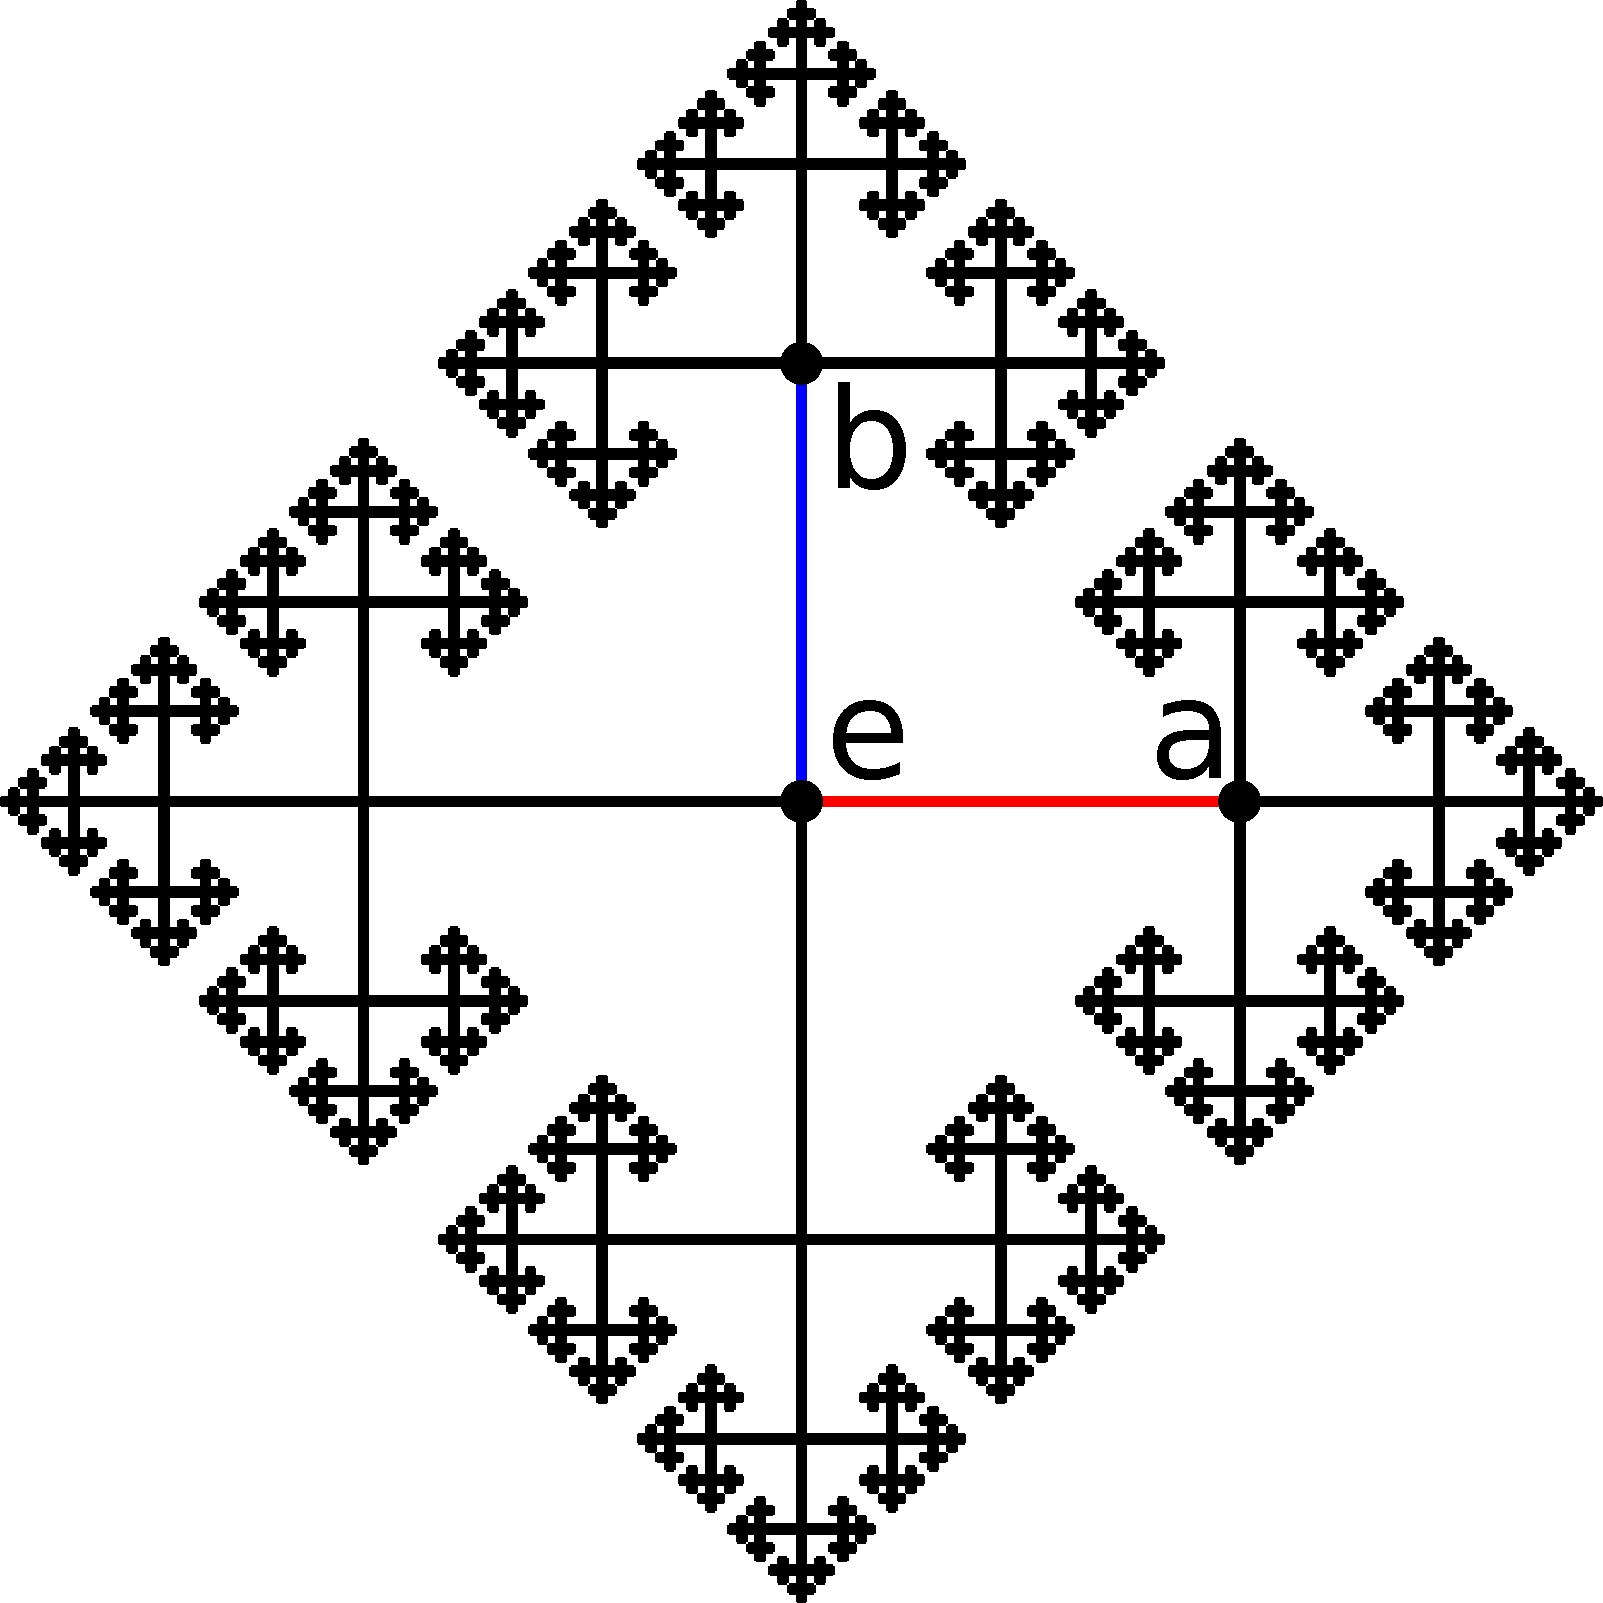
\includegraphics[scale=0.15]{figures/Cayley.pdf}
    \caption{This graph is the universal cover of the figure eight, which is $\Gamma=\bbS^1 \vee \bbS^1$. It is also the Cayley graph of the fundamental group of $\Gamma$, i.e., the free group with two generators $a$ and $b$, $\pi_1(\Gamma)=F(\{a,b\})\cong\bbZ\ast\bbZ$. \label{Fig. Cayley}}
\end{figure}

We can now use the theory of covering spaces to prove a very important basic theorem about free groups. 
\begin{thm}[Nielsen-Schreier]\index{Theorem!Nielsen-Schreier}\label{thm Nielsen-Schreier}
    Any subgroup of a free group is free.
\end{thm}
\begin{proof}
    Let $G$ be a free group. As we've seen, it can be realized as the fundamental group of a \emph{bouquet} $M=\bigvee \bbS^1$ of as many circles as there are generators in $G$. Given a subgroup $H\leq G$, there must exist a covering space $E\overset{\pi}{\to}M$ such that $H=\pi_\ast(\pi_1(E,p_0))$ and $\pi_\ast:\pi_1(E,p_0)\to H\subset \pi_1(M,x_0)$ is an isomorphism. However, any covering space of a graph is a graph (indeed,each edge incident with a vertex in the base can be uniquely lifted to the total space, these liftings are homeomorphisms, and doing so for all vertices gives the total space a structure of a graph). In particular, any covering space of a bouquet of circles is a bouquet of circles. This implies that the fundamental group of $E$ is free, and therefore $H$ is free.
\end{proof}
\begin{cor}
    If a subgroup of a free group of finite rank has finite index, then it is also of finite rank.
\end{cor}
\begin{proof}
    Indeed, if $H\leq G$ has finite index, it can be realized as the fundamental group of a finite covering graph of a finite bouquet of circles. But any such graph has a finitely generated fundamental group.
\end{proof}
\begin{thm}[Schreier formula]
    If $G$ is a free group of finite rank $r_G$ and $H \leq G$ is a subgroup of finite index $n$, then $H$ is free of rank $r_H=n(r_G-1)+1$.
\end{thm}
\begin{proof}
    Let $G=F(x_1,\ldots,x_{r_G})$. This follows from examining the covering graph constructed in Theorem~\ref{thm Nielsen-Schreier}. It has one vertex for each right coset $Hg$ and exactly $2r_G$ edges at each vertex ($r_G$ going in and $r_G$ going out) with the outgoing edge going from $Hg$ to $Hgx_i=(Hg)\cdot x_i$ labeled by the generator $x_i$. Therefore this graph has $V=n$ vertices and $E=nr_G$ edges. The fundamental group of this graph $\wt\Gamma$ is isomorphic to $H$ and is generated by $1-\chi(\wt\Gamma)=1-V+E=n(r_G-1)+1$ loops.
\end{proof}
\begin{cor}
    Let $\Gamma$ be a covering graph of $\bigvee_{i=1}^r \bbS^1$ (with $r>1)$ that corresponds to a subgroup generated by $r'>1$ generators. If $n=(r'-1)/(r-1)$ is a positive integer then $\Gamma$ has $n$ sheets, otherwise $\Gamma$ has infinitely many sheets.
\end{cor}
\begin{cor}
    The free group of two generators, $F(a,b)$, contains free subgroups of any integer rank $r_H$. 
\end{cor}
\begin{proof}
    The set of all words whose degree (the sum of the powers of all generators in it) equals $r_H$ is one such subgroup.

    Alternatively, we can simply notice that the space $\bbS^1\vee \bbS^1$ has covering spaces that are homeomorphic to $\bigvee_{i=1}^r \bbS^1$ for any $r$.
\end{proof}

\begin{example}[Covering spaces of $\bbS^1\vee \bbS^1$]
    Consider the ``figure eight'' space $M=\bbS^1\vee \bbS^1$. Its covering spaces are in one-to-one correspondence with conjugacy classes of subgroups of the free group $F(a,b)$ of two generators (one for each circle in $M$). By Theorem~\ref{thm Nielsen-Schreier}, any subgroup of a free group is free, so each covering space of $M$ is uniquely determined by a subset of $F(a,b)$ that contains no relations (e.g., the set $\{a^2,b^2,a^2b^2\}$ is redundant and should be replaced with $\{a^2,b^2\}$). The elements of this subset generate the image of $\pi_1(E,p_0)$ under the monomorphism $\pi_\ast$.

    Some examples of these covering spaces are given in Figures~\ref{fig:sixfold covering} and \ref{fig:coverings of 8}. The covering in Figure~\ref{fig:threefold-cover} is another one. It is instructive to observe which of the coverings in Figure~\ref{fig:coverings of 8} are regular, and how the subgroups corresponding to them are normal. It is similarly instructive to verify the Lifting Theorem~\ref{Lifting Theorem}: two different covering spaces of $M$ are covering spaces of each other (say with basepoints) only if the generators of the stabilizer of one of them can be expressed in terms of the generators of the other. For example, (11) is a covering space of (1) because  $b^nab^{-n}=(b^2)^{n/2}a(b^{-2})^{n/2}$ if $n$ is even and $b^nab^{-n}=(b^2)^{(n-1)/2}bab^{-1}(b^{-2})^{(n-1)/2}$ otherwise.

    (1) and (2), up to swapping $a$ and $b$, are all of the existing connected double covers (so there are three in total). (3) and (4) are the same covering space but with different basepoints, and one can see how the corresponding subgroups are conjugates of each other by an element that connects those two points, for example $b$.
\end{example}

\begin{figure}
    \centering
    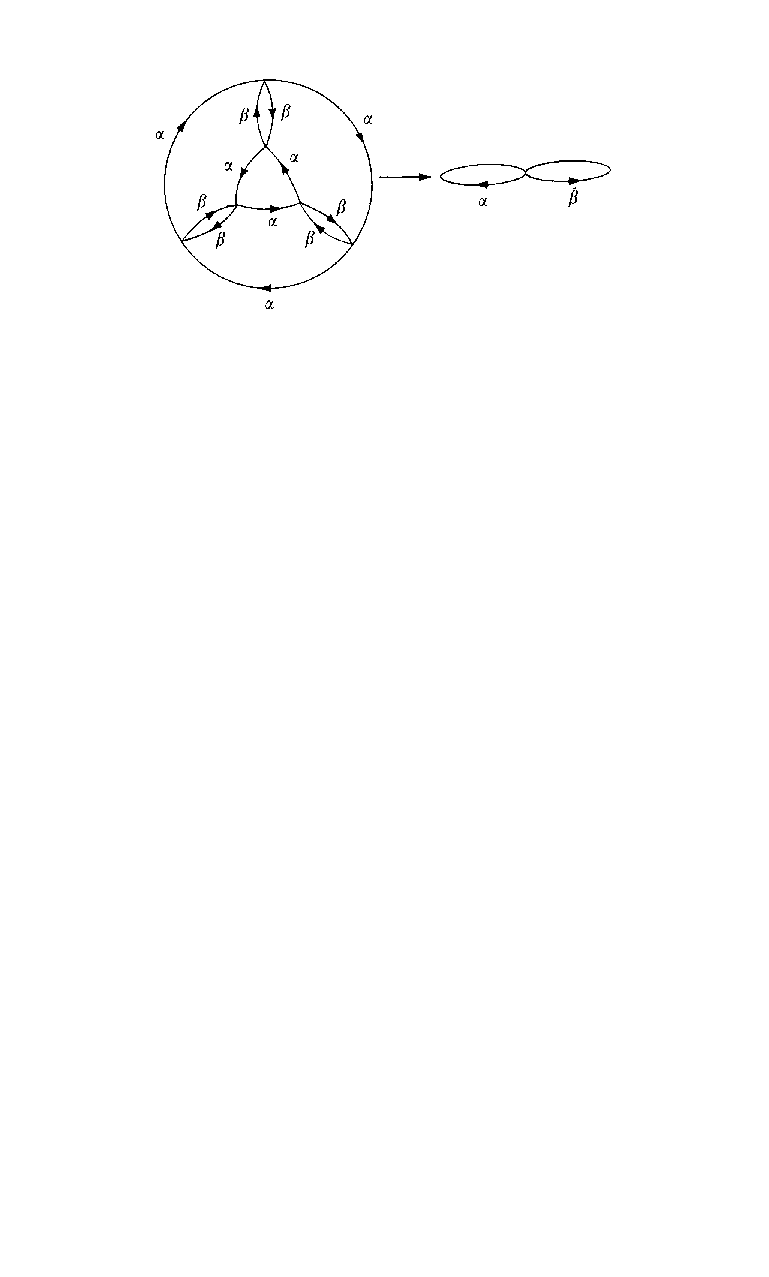
\includegraphics[width=0.6\textwidth]{figures/sixfold.pdf}
    \caption{A sixfold regular covering space of the figure eight. The fundamental group $\pi_1(E,p_0)$ is clearly generated by six loops. This makes it easy to guess that the stabilizer of any vertex is the normal subgroup of the free group $F(\alpha,\beta)$ generated by the six elements $\alpha^3,\beta^2,\left(\alpha\beta^{-1}\right)^2, \left(\alpha^{-1}\beta\right)^2, \alpha\beta^2\alpha^{-1}, \alpha^{-1}\beta^2\alpha$. To find the group of deck transformations, we factor the free group by this normal subgroup, which is equivalent to adding these six generators as relations. It is easy to check that these relations define the permutation group $\rmS_3=\langle a,b\mid a^2,b^2,ababab\rangle$. If we reversed the arrows on the inner triangle of $\alpha$'s, we'd get $\bbZ_2\times \bbZ_3$ instead. From \cite[Fig.~III-7]{Bredon}.}
    \label{fig:sixfold covering}
\end{figure}

\begin{figure}
    \centering
    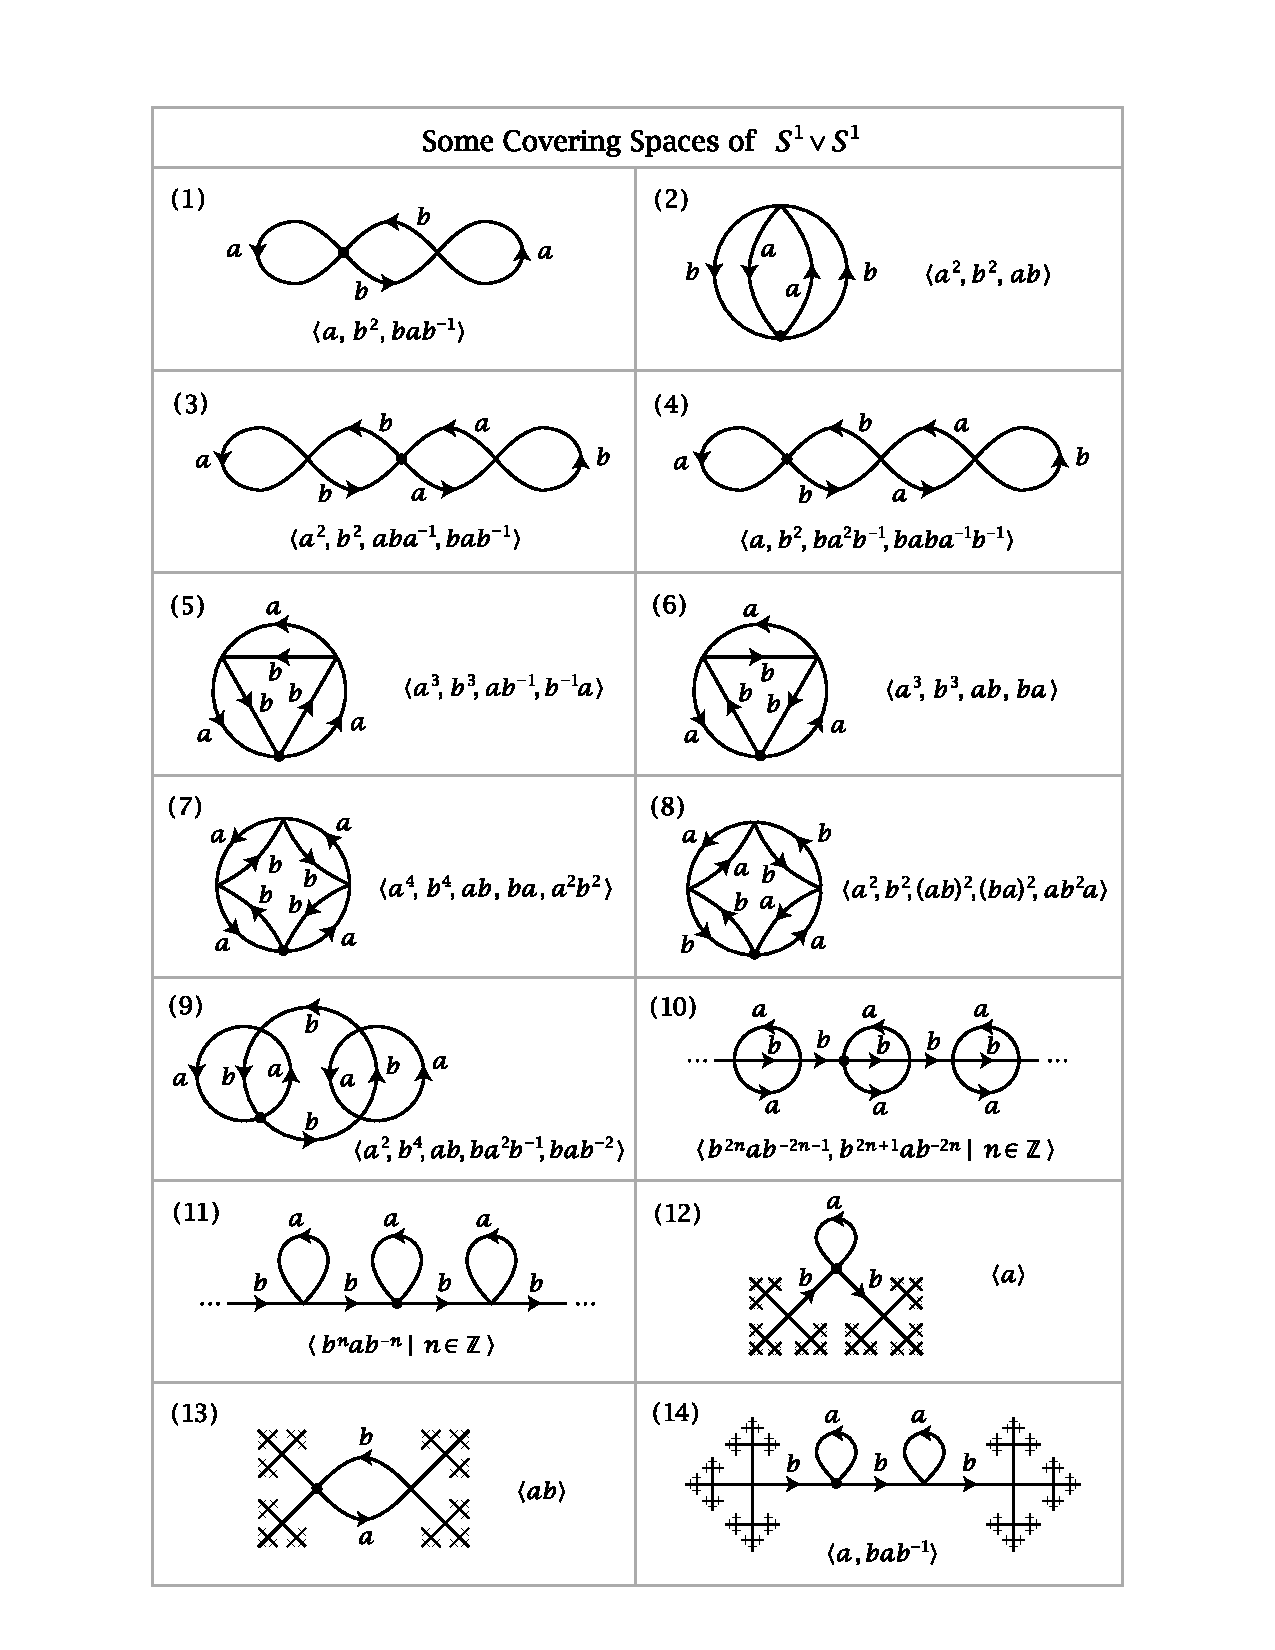
\includegraphics[width=0.67\textwidth]{figures/coverings_8.pdf}
    \caption{Examples of covering spaces of the figure eight space. Each one is a graph with a marked basepoint $p_0$ such that the neighborhood of each vertex locally looks the same as in the base space: two incoming edges (labeled $a,b$) and two outgoing (also labeled $a,b$). The label of an edge indicates which generator of $\pi_1(M)$ it is projected onto by $\pi$. Next to the space is the list of the generators of the local fundamental group $\pi_1(E,p_0)$ expressed in terms of $a,b$, which means that, viewed as part of $\pi_1(M)$, they generate the stabilizer $G_{p_0}=\pi_\ast(\pi_1(E,p_0))$. The number of sheets matches the index of this subgroup. Two vertices are related by a deck transformation iff their stabilizers coincide, otherwise the stabilizers are merely conjugate. For regular coverings (1,2,5,6,7,8,9,11), all stabilizers coincide and therefore are normal. From \cite[p.~58]{Hatcher}.}
    \label{fig:coverings of 8}
\end{figure}


\begin{xca}
    Show that the covering space of the figure eight space $M=\bbS^1\vee \bbS^1$ that corresponds to the normal subgroup generated by $a^2$, $b^2$, and $(ab)^4$ (where $a,b$ are the two generators of the free group $\pi_1(M)$) is regular, and describe what it looks like. \emph{Hint:} this subgroup has index 8, so it's an eight-fold covering.
\end{xca}

\begin{xca}
    Describe the covering space of the figure eight space that corresponds to the commutator subgroup of the free group of two generators. \emph{Hint:} $F(a,b)\slash [F(a,b),F(a,b)]=\bbZ^2$, so this covering space has a $\bbZ^2$-symmetry.
\end{xca}
\begin{xca}
    Identify in $\bbS^1$ the open upper and the open lower semicircle to a point. The resulting space $X$ has four points. Show $\pi_1(X)\cong \bbZ$. Does $X$ have a universal covering?
\end{xca}
\begin{xca}
    Show that the universal cover of $M_1\times M_2$ is $\wt M_1\times \wt M_2$.
\end{xca}
\begin{xca}[{{\cite[Exercise~B.7]{Hatcher}}}]
    If $G$ is a finitely generated free group and $N$ is a nontrivial normal subgroup of infinite index, show, using covering spaces, that $N$ is not finitely generated.
\end{xca}

\begin{example}
    $\widetilde{\bbT^n}=\bbR^n$, $\widetilde{\text{SO}_3}=\text{SU}_2=\bbS^3$, $\widetilde{\text{SO}}_{n>2}=\text{Spin}_n$, $\widetilde{\text{U}_n}=\text{SU}_n\times \bbR $.
\end{example}











\clearpage
\chapter{Homotopy Theory}

\section{Homotopy groups}

\begin{defn}[Homotopy groups]\index{Homotopy groups}
Pick the base points $\bullet\in \bbS^n$ and $x_0\in X$. The set of homotopy classes of maps $\gamma:\bbS^n\to X$ such that $\gamma(\bullet)=x_0$ forms the $n$-th homotopy group $\pi_n(X,x_0)=[\bbS^n;X]_\bullet$. For two such maps, define their product by first mapping $\bbS^n$ onto the wedge sum $\bbS^n\lor \bbS^n$ via contracting an arbitrarily chosen equator (which is homeomorphic to $\bbS^{n-1}$) into one point, then apply $\gamma_1$ and $\gamma_2$ to the two hemispheres respectively, making the equator point the base point for them.

For $n=0$, $\pi_0(X)$ is defined as the set of path-connected components of $X$ (which is also the set of homotopy classes of pointed maps $\bbS^0\to X$) but does not have a natural group structure.
\end{defn}

\begin{xca}
\begin{enumerate}
    \item The above definition is consistent and the resulting homotopy classes don't in fact depend on the choice of an equator. In fact, in natural terms, this group operation is exactly the coproduct on the category of pointed spaces, given by the wedge sum $\gamma_1\lor\gamma_2:\bbS^n\lor \bbS^n\to X$ (a.k.a. \emph{concatenation}).
    \item All homotopy groups for different $x_0$ are isomorphic.
\end{enumerate}
\end{xca}


\begin{prop}[Functoriality of $\pi_n$]
    Any pointed continuous map $f:X\to Y$ induces a homomorphism of the homotopy groups $f_\ast:\pi_n(X,x_0)\to \pi_n(Y,y_0)$, and $(g\circ f)_\ast=g_\ast\circ f_\ast$. In other words, we have a \emph{functor} $\pi_n:\mathsf{Top}_\bullet\to \mathsf{Gr}$.
\end{prop}

\begin{thm}
Homotopy groups $\pi_n$, $n\geq 1$, are homotopy invariants, i.e., if $X\simeq Y$ are two homotopy equivalent path connected spaces, then $\pi_n(X,x_0)\cong\pi_n(Y,y_0)$.
\end{thm}
\begin{proof}
Exercise. Also see \cite{Hatcher}.
\end{proof}
\begin{cor}
    $\pi_n$ descends to a functor $\pi_n:\mathsf{hTop}_\bullet\to \mathsf{Gr}$ on the category $\mathsf{hTop}_\bullet$, in which the morphisms are the homotopy classes of pointed continuous maps modulo homotopy relative to the base point. In particular, homotopy equivalent spaces have isomorphic homotopy groups.
\end{cor}

\begin{thm}
For $n\geq 2$, all groups $\pi_n(X,x_0)$ are abelian.
\end{thm}
\begin{proof}
Follows from Proposition~\ref{suspension maps prop} and the fact that $\bbS^n=\Sigma\Sigma \bbS^{n-2}$ for $n\geq 2$. We have $[\bbS^n,Y]=[\Sigma\Sigma \bbS^{n-2},Y]=[\Sigma \bbS^{n-2}, \Omega Y]$, which is abelian.
\end{proof}

Another very important connection between homotopy groups and suspension will be discussed when we prove Freudenthal's Suspension Theorem~\ref{thm 6.4.7 tomDieck freudenthal}.

\begin{comment}
\PRLsep
\begin{center}
  {\red Lecture 4 on 30 Nov 2018 ended here}
\end{center}
\end{comment}



\section{Exact sequence of homotopy groups}

\begin{defn}[Topological triple]
    A triple $(X,A,B)$ is a topological space $X$ with a pair of subspaces $A\subset B\subset X$. When $B=\bullet$ is a point, the triple is also called a pointed pair.
\end{defn}

\begin{defn}[Relative homotopy groups]\index{Relative homotopy groups}\index{Homotopy groups!relative}
        For a pointed pair $(X,A,\bullet)$ and $n\geq 1$ the relative homotopy group $\pi_n(X,A,\bullet)$ is the set of homotopy classes of triples $\pi_n(X,A,\bullet)=[(\bbD^n,\bbS^{n-1},\bullet);(X,A,\bullet)],$
        where $\bbD^n$ is the $n$-disk, $\bbS^{n-1}$ is its boundary, and the homotopies are through pointed maps that take $\bbS^{n-1}$ into $A$. Note that this is \emph{not} the same as homotopies relative to $\bbS^{n-1}$.
\end{defn}
These are groups with the same multiplication operation and they are still abelian for $n\geq 3$ because $[(\Sigma X,\Sigma A);(Y,B)]=[( X, A);(\Omega Y,\Omega B)]$.
\begin{prop}[Compression criterion]\label{prop: compression criterion}
    A map $f:(\bbD^n,\bbS^{n-1},\bullet)\to (X,A,\bullet)$ represents the identity in $\pi_n(X,A,\bullet)$ iff it is homotopic $\rel \partial \bbD^n\cong \bbS^{n-1}$ to a map whose image is contained in $A$.
\end{prop}
\begin{proof}
    For necessity, a map whose image is contained in $A$ can be composed with a deformation retraction of $\bbD^n$ onto the basepoint to give a homotopy to a trivial map. Conversely, if $[f]=e$ via a homotopy $H:\bbD^n\times I\to X$, then by restricting $H$ to a family of $n$-disks in $\bbD^n\times I$ starting with $\bbD^n\times \{0\}$ and ending with the disk $\bbD^n\times\{1\}\cup \bbS^{n-1}\times I$, all the disks in the family having the same boundary, then we get a homotopy from $f$ to a map onto $A$, stationary on $\bbS^{n-1}$. This is a homotopy relative to $A$.
\end{proof}

Any map $f:(X,A,x_0)\to (Y,B,y_0)$ induces maps $f_\ast :\pi_n(X,A,x_0)\to \pi_n(Y,B,x_0)$ which are homomorphisms for $n\geq 2$ and have properties analogous to those in regular homotopy: $(f\circ g)_\ast=f_\ast\circ g_\ast$, $\mathrm{id}_\ast=\mathrm{id}$, and $f_\ast=g_\ast$ if $f\sim g$ through maps of pointed pairs $(X,A,x_0)\to(Y,B,y_0)$.

In particular, the inclusions $i:(A,x_0)\hookrightarrow(X,x_0)$ and $j:(X,x_0,x_0)\hookrightarrow (X,A,x_0)$ induce such homomorphisms. Moreover, there is a third special homomorphisms that connects homotopy groups in adjacent degrees.

\begin{defn}[Boundary operator for homotopy]
    The inclusion of the boundary $\bbS^{n-1}\hookrightarrow \bbD^n$ induces restrictions of maps $f:(\bbD^n,\bbS^{n-1},s_0)\to (X,A,x_0)$ to the boundary, i.e., $\partial f=\restr{f}{\partial \bbD^n}$. For $n\geq 2$ this operator defines a homomorphism of relative homotopy groups.
\end{defn}

\begin{defn}[Exact sequence]
    Let $\calC$ be a category in which the notions of kernels and images of morphisms are well-defined. For now we assume that it is a concrete category, so kernels and images are understood as subsets of the domain and codomain, respectively. Next let there be a (finite or infinite) sequence of morphisms
    \[\cdots\to X\overset{f}{\to } Y\overset{g}{\to} Z\to \cdots \]
    We say that this sequence is exact at $Y$ if $\im f=\ker g$.
\end{defn}
\begin{example}
    In the category of pointed sets (or topological spaces etc.), kernels can be defined as the preimages of the basepoint. Exactness then amounts to $\im f=g^{-1}(*)$.

    Usually we will be concerned with the case $\calC=\mathsf{Gr}$.
\end{example}
\begin{defn}[Short exact sequence]
    A short exact sequence is a sequence of the form
    \[0\to X\overset{f}{\to } Y\overset{g}{\to} Z\to 0,\]
    where $0$ is a zero object in $\calC$.

    The exactness at $X$ is equivalent to $f$ being a monomorphism. Exactness at $Z$ is equivalent to $g$ being an epimorphism. The exactness at $Y$ essentially says that $Z\cong Y\slash \im f=Y\slash \ker g\cong Y\slash X$. In the category of groups this is just the first isomorphism theorem.
\end{defn}

\begin{example}
    If the short exact sequence is even shorter, e.g.
    \[0\to X\overset{f}{\to } Y\to 0,\]
    then its exactness is equivalent to $f$ being an isomorphism.
\end{example}

\begin{thm}[Long exact sequence of homotopy groups]\index{Long exact sequence!of homotopy groups}\label{thm long exact seq of homotopy}
    The sequence of homomorphisms
    \[\cdots \to \pi_n(A,x_0)\overset{i_\ast}{\to}\pi_n(X,x_0)\overset{j_\ast}{\to}\pi_n(X,A,x_0)\overset{\partial}{\to}\pi_{n-1}(A,x_0)\to \cdots \to \pi_0(X,x_0)\]
    is \emph{exact}. Near the end of the sequence, where the group structure is not defined, the ``kernel'' is the path-connected component of $x_0$.
\end{thm}
\begin{proof}
    In fact we will prove the long exact sequence of a pointed triple $(X,A,B,x_0)$ with $x_0\in B\subset A\subset X$:
    \begin{multline}
        \cdots \to \pi_n(A,B,x_0)\overset{i_\ast}{\to}\pi_n(X,B,x_0)\overset{j_\ast}{\to}\pi_n(X,A,x_0)\overset{\partial}{\to}\pi_{n-1}(A,B,x_0)\to \cdots \\ \to \pi_1(X,A,x_0).
    \end{multline}
    The boundary operator for triples is defined as the composition $\partial:\pi_n(X,A)\overset{\partial}{\to} \pi_{n-1}(A)\overset{i_\ast}{\to} \pi_{n-1}(A,B)$ where $i:B\hookrightarrow A$ is the inclusion map. When $B=\{x_0\}$ this reduces to the exact sequence of the pointed pair $(X,A,x_0)$, though the latter sequence continues for two more steps to $\pi_0(X,x_0)$.

    \emph{Exactness at} $\pi_n(X,B,x_0)$: First note that the composition $j_\ast\circ i_\ast$ is trivial since every map $(\bbD^n,\bbS^{n-1},s_0)\to (A,B,x_0)$ represents zero in $\pi_n(X,A,x_0)$ by the compression criterion. To see that $\ker j_\ast \subset \im i_\ast$, let $f:(\bbD^n,\bbS^{n-1},s_0)\to (X,B,x_0)$ represent the trivial element in $\pi_n(X,A,x_0)$. Then by the compression criterion again, $f$ is homotopic $\rel \bbS^{n-1}$ to a map with image in $A$, hence $[f]\in \pi_n(X,B,x_0)$ is in the image of $i_\ast$.

    \emph{Exactness at} $\pi_n(X,A,x_0)$: The composition $\partial\circ j_\ast$ is zero since the restriction of a map $(\bbD^n,\bbS^{n-1},s_0)\to (X,B,x_0)$ to $\bbS^{n-1}$ has image lying in $B$, and hence represents the trivial class in $\pi_{n-1}(A,B,x_0)$. Conversely, suppose the restriction of $f:(\bbD^n,\bbS^{n-1},s_0)\to (X,A,x_0)$ to $\bbS^{n-1}$ represents the trivial element $\pi_{n-1}(A,B,x_0)$. Then $\restr{f}{\bbS^{n-1}}$ is homotopic to a map with image in $B$ via a pointed homotopy $H:\bbS^{n-1}\times I \to A$. We can tack $H$ onto $f$ to get a new map $(\bbD^n,\bbS^{n-1},s_0)\to (X,B,x_0)$ which, as a map $(\bbD^n,\bbS^{n-1},s_0)\to (X,A,x_0)$, is homotopic to $f$ by the homotopy that tacks on increasingly longer initial segments of $H$. So $[f]\in \im j_\ast$.

    \emph{Exactness at} $\pi_n(A,B,x_0)$: The composition $i_\ast \circ \partial$ is trivial since the restriction of a map $f:(\bbD^{n+1},\bbS^n,s_0)\to (X,A,x_0)$ to $\bbS^n$ is homotopic $\rel s_0$ to a constant map via $f$ itself (via a contraction of $\bbS^n$ onto $s_0$ inside $\bbD^n$). The converse is easy if $B$ is a point, since the nullhomotopy $f_t:(\bbD^n,\bbS^{n-1})\to (X,x_0)$ of $f_0:(\bbD^n,\bbS^{n-1})\to (A,x_0)$ gives a map $F:(\bbD^{n+1},\bbS^n,s_0)\to (X,A,x_0)$ with $\partial([F])=[f_0]$. Thus the proof is finished in this case. 
    
    For a general $B$, let $f:(\bbD^{n},\bbS^{n-1},s_0)\to (A,B,x_0)$ be in the kernel of $i_\ast$ and let $F:\bbD^n\times I\to X$ be a corresponding nullhomotopy of $f$ through maps $(\bbD^n,\bbS^{n-1},s_0)\to (X,B,x_0)$. It is then clear that $F$ can be viewed as a map $\bbD^{n+1}\to X$ which restricts to $f$ on $\bbD^n\times \{0\}$, and maps the rest of the boundary into $B\subset A$, which makes $f$ the boundary of some map $(\bbD^{n+1},\bbS^n,s_0)\to (X,A,x_0)$.
\end{proof}



\section{\texorpdfstring{$CW$}{CW}-complexes}

\begin{defn}[$CW$-complex]\index{$CW$-complex}\index{Cell complex}
    A cellular structure on a set $X$ is a family $\calF $ of \textit{characteristic mappings} $f_\alpha^n:\bbD^n\to X$, where $n=0,1,2,\ldots$ and $\alpha\in A_n$ (some indexing sets), such that the following conditions hold. Let $X^{(n)}$ denote the union of images of mappings $f_\alpha^k, k\leq n$. Also $X^{(-1)}=\varnothing$.
    \begin{enumerate}
        \item For every $n$, $\bigsqcup_\alpha f_\alpha^n$ maps $\bigsqcup_\alpha \Int \bbD^n$ \emph{injectively} to $X\setminus X^{(n-1)}$. Here, we put $\Int \bbD^0=\bbD^0$.
        \item Every $f_\alpha^n$ maps $\partial \bbD^n$ to $X^{(n-1)}$.
        \item $X=\bigcup_n X^{(n)}$.
    \end{enumerate}
    
    A $CW$-complex is a Hausdorff topological space with a $CW$-structure such that the topology coincides with the final topology defined by $\calF $, also called the \emph{weak topology}\index{Weak topology}: $A\subset X$ is open iff $A\cap X^{(n)}$ is open in $X^{(n)}$ for each $n$.

    The restrictions $\partial f_\alpha^n=\restr{f_\alpha^n}{\partial \bbD^n}$ are called the \textit{attaching maps}. The subsets $X^{(n)}\subset X$ are called the $n$-skeleta of $\calF $. The images $f_\alpha^n(\bbD^n)$ are referred to as the \textit{closed cells} and $f_\alpha^n(\Int  \bbD^n)$ as \textit{open cells} (even though these are actually closed or open only as subspaces of $X^{(n)}$!). A $CW$-complex $(X,\calF )$ is said to be pointed if $X$ is pointed and the basepoint is a $0$-cell. A subcomplex is a subspace $X'\subset X$ endowed with the relative topology, together with a subfamily $\calF '\subset\calF $ such that $(X',\calF ')$ is a $CW$-complex. The highest dimension of a cell in a complex is called its dimension. A $CW$-complex is called finite if it is finite-dimensional and has a finite number of cells.
\end{defn}

We will typically work with finite $CW$-complexes, but infinite-dimensional ones will be useful as well.

\begin{rem}
The acronym $CW$ refers to the following properties.
\begin{enumerate}
    \item Closure-finiteness: every closed cell meets only finitely many open cells, which we will prove in Proposition~\ref{prop 8.1 Bredon}.
    \item Weak topology: $X$ carries the final topology defined by the family $\calF $.
\end{enumerate}
A  more general concept of cellular complexes drops these requirements. Note that, due to the inductive definition of $CW$-complexes as a collection of attaching maps, we get (C) automatically.
\end{rem}

% The following proposition shows that the weak topology induced by any \emph{finite} $CW$-structure consisting of continuous characteristic maps  on a Hausdorff space coincides with the original topology.

% \begin{prop}[{{\cite[Prop.~3.1.9]{RS2}}}]\label{prop 3.1.9 RS2}
%     Let $X$ be a Hausdorff space and let $\calF $ be a finite $CW$-structure on $X$. For $\calF $ to make $X$ into a $CW$-complex it suffices that every $f_\alpha^n\in\calF $ be continuous.
% \end{prop}
% \begin{proof}
%     We show that a subset $A \subset X$ is closed iff $(f_\alpha^n)^{-1}(A)\subset \bbD^n$ is closed for all $n$ and $\alpha$. The `only if' direction is obvious. To prove the `if' direction, assume that $(f_\alpha^n)^{-1}(A)$ is closed for all $n$ and $\alpha$. Since a continuous mapping from a compact space to a Hausdorff space is closed, it follows that $f_\alpha^n((f_\alpha^n)^{-1}(A))\subset X$ is closed for all $n$ and $\alpha$. Since $A$ is the union over all these subsets, and since their number is finite, we conclude that $A$ is closed.
% \end{proof}

Every $CW$-complex therefore can be thought of as a \emph{decomposition} of a Hausdorff space $X$ into a disjoint union of open cells of various dimensions. The space $X$, up to homeomorphism, can be inductively reconstructed from its $CW$-structure as follows. First, $X^{(0)}$ is a discrete set of points. Next, given an $(n-1)$-skeleton $X^{(n-1)}$, we can obtain $X^{(n)}$ by taking a disjoint union of $n$-disks $\sqcup_\alpha \bbD^n$ and identifying their boundaries with points of $X^{(n-1)}$ via the attaching maps $\partial f_\alpha^n:\partial \bbD^n\to X^{(n-1)}$, which are required to be continuous. The space $X$ is then the inductive union of all skeleta with the final topology.


\begin{example}
    \begin{enumerate}
        \item A graph is nothing but a $0$- or $1$-dimensional cell complex.
        \item The infinite bouquet $\bigvee_{i=1}^\infty \bbS^1$ is not a $CW$-complex because the basepoint has to meet infinitely many $1$-cells.
        \item The sphere $\bbS^n$ admits a $CW$-structure with one $0$-cell and one $n$-cell. The characteristic maps can be chosen as 
        \[f^0(*)=e_1,\quad f^n(x)=(2|x|^2-1,2\sqrt{1-|x|^2}x).\]
        Another useful $CW$-structure on the sphere has two cells in each dimension up to $n$. Its characteristic maps are
        \[f^0_\pm (*)=\pm e_1\,\quad f^k_\pm(x)=(x,\pm\sqrt{1-|x|^2},0,\ldots,0).\]
        The two $k$-cells are given by
        \[\{(x_1,\ldots,x_{k+1},0,\ldots,0)\in \bbS^n:\pm x_{k+1}\geq 0\}.\]
        \item The closed $n$-disk $\bbD^n$ has a tautological $CW$-structure with one $n$-cell. It is however sometimes convenient to have the boundary $\bbS^{n-1}$ as a subcomplex. This can be achieved by just adding either one of the two $CW$-structures of $\bbS^{n-1}$ above.
        \item The wedge sum of two $CW$-complexes $(X_1,\calF _1)\vee (X_2,\calF _2)$ carries a natural $CW$-structure $\calF _1\cup \calF _2$.
        \item The direct product $(X_1,\calF _1)\times (X_2,\calF _2)$ has a $CW$-structure with elements $(f_{1i}^n\times f_{2j}^m)\circ p_{n+m}$ where $p_{n+m}:\bbD^{n+m}\to \bbD^n\times \bbD^m$ is some chosen homeomorphism. This makes sense, because, as a homeomorphism, $p_{n+m}$ maps the boundary $\bbS^{n+m-1}$ of $\bbD^{n+m}$ onto the boundary $(\bbS^{n-1}\times \bbD^m)\cup (\bbD^n\times \bbS^{m-1})$ of $\bbD^n\times \bbD^m$. For example, the direct product of two copies of $\bbS^1$ with one cell in dimensions $0$ and $1$ yields a $CW$-structure on the torus $\bbT^2$ with one $0$-cell, one $2$-cell, and two $1$-cells. Note that in general the topology on the product complex need not coincide with the product topology, but it does when the complexes are locally finite (i.e., every point has a neighborhood that overlaps only with finitely many open cells -- such spaces are also paracompact).
    \end{enumerate}
\end{example}

\begin{prop}[{{\cite[Prop.~3.1.11]{RS2}}}]\label{prop 3.1.11 RS2}
    Let $(X,\calF )$ be a $CW$-complex, $Y$ a topological space, and $f:X\to Y$ a map. Then $f$ is continuous iff its restrictions $f\circ f_\alpha^n$ to each cell are continuous.
\end{prop}
\begin{proof}
    This is nothing but the universal property of the final topology, but let us walk through the argument. Only the sufficiency is not obvious. Let $V\subset Y$ be open. By assumption, $(f\circ f_\alpha^n)^{-1}(V)$ is open in $\bbD^n$ for all $n$ and $\alpha$. Since $(f\circ f_\alpha^n)^{-1}(V)=(f_\alpha^n)^{-1}(f^{-1}(V))$, then $f^{-1}(V)\subset X$ is open by virtue of being the image of an open set under a quotient map (and all quotient maps are open by definition). 
\end{proof}

% \begin{prop}[{{\cite[Prop.~3.1.12]{RS2}}}]\label{prop 3.1.12 RS2}
%     Let $(X,\calF )$ be a $CW$-complex, $Y$ a topological space, and $f_n:X^{(n)}\to Y,n=0,1,\ldots$ a family of continuous mappings satisfying $\restr{f_{n+1}}{X^{(n)}}=f_n$ for all $n$. Then there exists a unique mapping $f:X\to Y$ that restricts to $f_n$ on $X^{(n)}$ for all $n$, and $f$ is continuous.
% \end{prop}
% \begin{proof}
%     Since the assumption implies that $\restr{f_{m}}{X^{(n)}}=f_n$ for all $m>n$, and since $X$ is the union of $n$-skeleta, we can define $f$ by $\restr{f}{X^{(n)}}=f_n$. Uniqueness is then obvious. To check continuity, observe that for all $n,i$ and $x\in \bbD^n$, we have $f(f_i^n(x))=f_n(f_i^n(x))$. It follows that $f\circ f_i^n$ is continuous for all $n$ and $i$ and hence, by Proposition~\ref{prop 3.1.11 RS2}, that $f$ is continuous.
% \end{proof}

\begin{prop}[{{\cite[Prop.~8.1]{Bredon}}}]\label{prop 8.1 Bredon}
    If $X$ is a $CW$-complex then
    \begin{enumerate}[label=(\arabic*)]
        \item if $A\subset X$ has no two points in the same open cell, then $A$ is closed and discrete;
        \item if $K\subset X$ is compact then $K$ is contained in a finite union of open cells;
        \item each cell of $X$ is contained in a finite subcomplex of $X$ (i.e., the cell complex is \emph{``closure finite''}).
    \end{enumerate}
\end{prop}
\begin{proof}
    We will first show that all three statements are equivalent to each other.
    
    $(1)\implies (2)$. If $K\subset X$ is compact then let $A\subset K$ be a set of points, one from each open cell touching $K$. By (1) $A$ is closed, hence compact, and discrete. Hence $A$ is finite. But that means $K$ is contained in a finite union of open cells as claimed.

    $(2)\implies(3)$. In fact, for a cell $\alpha$, we will only use (2) for the set $K$ which is the image of the attaching map $f_{\partial \alpha}:\partial \bbD^n\to X^{(n-1)}$ of that cell, and the images of attaching maps of smaller-dimensional cells. Statement (2) implies that $X_\sigma=f_\sigma(\bbD^n)$ is contained in a finite union of open cells, and by construction all of these are of smaller dimension except for $U_\sigma=f_\sigma(\Int \bbD^n)$ itself. By the same token each of these lower-dimensional closed cells is contained in a finite union of open cells of even lower dimension (except for open the cell itself), and so on. This reasoning obviously must come to an end with $0$-cells in a finite number of steps, and, at that stage, the union of the cells produced a finite subcomplex.

    $(3)\implies(1)$. Consider the intersection of $A$ with a closed cell. By (3) this is contained in a finite subcomplex. Since $A$ has at most one point in common with any open cell this intersection must be finite, and hence closed. For any point $x\in A$, the set $A\setminus\{x\}$ satisfies the hypothesis for $A$, and so it must also be closed. Hence $\{x\}$ is open in $A$, so $A$ is discrete.

    Finally, we put all this together. Statement (1) clearly holds for $X^{(0)}$ (it must be discrete because it has the final topology of maps of points). Suppose we know (1) for the $n$-skeleton $X^{(n)}$. Then we also have (2) for $X^{(n)}$. In turn, we get (3) for $X^{(n)}$. But the proof of $(2)\implies(3)$ for a particular $k$-cell only used (2) for subsets of $X^{(k-1)}$. Thus we actually have (3) for $X^{(n+1)}$. Thus we also have (1) for $X^{(n+1)}$. Consequently, we have all three statements for $X^{(n)}$ for all $n$. But any cell is in some $X^{(n)}$, and so we know (3) for $X$ itself, and this implies (1) then (2) for $X$.
\end{proof} 
\begin{cor}
    The boundary of each cell is contained in finitely many closed cells of lower dimensions.
\end{cor}

\begin{thm}[{{\cite[Thm.~8.2]{Bredon}}}]\label{thm 8.2 Bredon}
    A compact subset of a $CW$-complex is contained in a finite subcomplex.
\end{thm}
\begin{proof}
    Let $K\subset X$ be compact. By (2) of Proposition~\ref{prop 8.1 Bredon}, $K$ is contained in a union of a finite number of open cells. By (3) of the same Proposition, each of these is contained in a finite subcomplex. The union of this finite number of finite subcomplexes is a finite subcomplex containing $K$.
\end{proof}

\begin{cor}\label{cor direct limit of pi_n for CW}
    If $X_1\hookrightarrow X_2\hookrightarrow \cdots$ is an infinite sequence of inclusions of $CW$-subcomplexes, then 
    \[\pi_n(\colimit X_i)=\colimit \pi_n(X_i).\]
\end{cor}
\begin{proof}
    Let $X=\colimit X_i=\bigcup X_i$ be the limiting $CW$-complex. Since $\bbS^n$ is compact, its continuous image in $X$ under any representative of an element of $\pi_n(X)$ is compact and thus contained in a finite subcomplex. Therefore every element of $\pi_n(X)$ is contained in $\pi_n(X_k)$ for some $k$ and hence in the directed colimit $\colimit \pi_n(X_i)$. Conversely, every element of this colimit is represented by some element of $\pi_n(X_k)$ for some $k$ by the explicit construction of the colimit.
\end{proof}




\begin{prop}
    A $CW$-complex is locally compact (every point has an open neighborhood contained in a compact set) iff it is locally finite (every point has an open neighborhood contained in a finite union of cells).
\end{prop}
\begin{proof}
    Exercise.
\end{proof}



\begin{defn}[Directed system, Direct limit]\index{Direct limit}
    A directed system of topological spaces consists of a directed set $(A,\leq)$ (a poset such that for all $a,b\in A$ there exists $c\in A$ such that $a\leq c$ and $b\leq c$), a topological space $X_\alpha$ for every $\alpha \in A$ and a continuous mapping $f_{\beta\alpha}:X_\alpha\to X_\beta$ for every pair $\alpha\leq\beta$ such that $f_{\alpha\alpha}=\id_{X_\alpha}$ and $f_{\gamma\beta}\circ f_{\beta\alpha}=f_{\gamma\alpha}$ for all $\alpha\leq\beta\leq \gamma$. The direct limit (\textit{colimit})
    \[X=\colimit X_\alpha\]
    of the directed system $\{X_\alpha,f_{\beta\alpha}\}$ is (up to homeomorphism) the topological quotient of the disjoint union $\bigsqcup_{\alpha\in A} X_\alpha$ with respect to the equivalence relation that $x\in X_\alpha$ is equivalent to $y\in X_\beta$ iff $\gamma\in A: f_{\gamma\alpha}(x)=f_{\gamma\beta} (y)$. Composition of the natural inclusions $X_\alpha\hookrightarrow \bigsqcup_\alpha X_\alpha$ with the quotient map yields continuous mappings
    \[\varphi_\alpha:X_\alpha\to X\]
    and the topology of $X$ coincides with the final topology defined by these maps. That is, a subset of $X$ is open iff its preimage under $\varphi_\alpha$ is open in $X_\alpha$ for all $\alpha$. In other words, the direct limit space is the set-theoretic direct limit with the final topology for the maps $\varphi_{\alpha}$.
\end{defn}

Direct limits are nothing but a generalization of pushouts to infinite families of objects, and will come up again in a more general categorical setting when we discuss homological algebra.


\begin{prop}[{{\cite[Prop.~3.1.14]{RS2}}}]\label{prop 3.1.14 RS2}
    Let $\{X_\alpha,f_{\beta\alpha}\}$ and $\{Y_\alpha,g_{\beta\alpha}\}$ be directed systems of topological spaces over the same index set $A$ and let $X$ and $Y$, respectively, be the direct limits. Every family of continuous mappings $h_\alpha:X_\alpha\to Y_\alpha$ satisfying $h_\beta \circ f_{\beta\alpha}=g_{\beta\alpha}\circ h_\alpha$ whenever $\alpha\leq \beta$ descends to a continuous mapping $h:X\to Y$.
\end{prop}

\begin{prop}[{{\cite[Prop.~3.1.15]{RS2}}}]\label{prop 3.1.15 RS2}
    Let $\{X_\alpha,f_{\beta\alpha}\}$ be a directed system of topological spaces and let $X$ be the direct limit. If for some $i$ one has $\pi_i(X_\alpha)=0$ for almost all (i.e., all but finitely many) $\alpha$, then $\pi_i(X)=0$.
\end{prop}


\begin{thm}[$CW$ Construction Theorem {{\cite[Thm.~5.20]{LeeTop}}}]
    Suppose $X_0\subset X_1\subset\cdots \subset X_{n}\subset $ is a sequence of topological spaces satisfying the following conditions:
    \begin{enumerate}[label=(\roman*)]
        \item $X_0$ is a nonempty discrete space.
        \item For each $n\geq 1$, $X_n$ is obtained from $X_{n-1}$ by attaching a (possibly empty) collection of $n$-cells.
    \end{enumerate}
    Then $X=\bigcup_n X_n$ has a unique topology coherent with the family $\{X_n\}_n$ (i.e., it is the final topology for the inclusions $X_n\hookrightarrow X$), and a unique cell decomposition making it into a $CW$-complex whose $n$-skeleton is $X_n$ for each $n$.
\end{thm}
\begin{proof}
    The uniqueness of the topology coherent with $\{X_n\}_n$ and of the cell decomposition is practically obvious. Finally, in the case of infinitely many cells one needs to check that $X$ is closure-finite and has the weak topology. See {{\cite[Thm.~5.20]{LeeTop}}} for full details.
\end{proof}

\begin{cor}
    The family of skeleta $X^{(k)}$ of a $CW$-complex together with the natural inclusion maps $f_{lk}:X^{(k)}\hookrightarrow X^{(l)}$ for $k\leq l$ forms a directed system of spaces. The direct limit of this system is homeomorphic to $X$: 
    \[X\cong \colimit X^{(n)}.\]
\end{cor}


\begin{example}[$\bbR^\infty$]\index{$\bbR^\infty$}\label{R-infty}
    By including $\bbR^n\hookrightarrow \bbR^{\bbN }$ via $x=(x_1,\ldots,x_n)\mapsto (x_1,\ldots,x_n,0,0,\ldots)$, we can take the direct limit
    \[\bbR^\infty=\colimit \bbR^n.\]
    This space consists of sequences of reals with only finitely many nonzero elements. The final topology on this space is strictly finer than the subspace topology inherited on it from the direct product topology on $\bbR^{\mathbb{N}}$.\footnote{The direct product topology on $\prod_\alpha X_\alpha$ is the coarsest topology under which the natural projections $\prod_\alpha X_\alpha\overset{\mathrm{pr}_\alpha}{\to} X_\alpha$ are continuous, and it is generated by sets of the form $\prod_\alpha U_\alpha$ where $U_\alpha\subset X_\alpha$ is open and for almost all $\alpha$, $U_\alpha=X_\alpha$.} In fact, $\bbR^\infty$ itself is not open as a subset of $\bbR^{\mathbb{N}}$.
\end{example}

\begin{example}[$\bbS^\infty$]\index{$\bbS^\infty$}\label{S-infty}
    Since we can obtain $\bbS^n$ from $\bbS^{n-1}$ by attaching two cells, we can take the direct limit
    \[\bbS^\infty=\colimit \bbS^n.\]
    This space includes every sphere $\bbS^n$ as a subcomplex. By the above theorem, $\pi_n(\bbS^\infty)=0$ for all $n$, however let us show the stronger result that $\bbS^\infty$ is contractible.

    The space $\bbR^\infty$ has a norm inherited from Euclidean norms on $\bbR^n$, which is simply $|x|=\sqrt{\sum_{i=1}^\infty x_i^2}$. The unit sphere under this norm is clearly a union of regular finite-dimensional spheres embedded into each other at the equator, which is $\bbS^\infty$. First, define the homotopy $f_t:\bbR^\infty\to \bbR^\infty$ by 
    \[f_t(x)=(1-t)x+tTx,\label{eq contracting homotopy S-inf}\]
    where $T(x_1,x_2,\ldots)=(0,x_1,x_2,\ldots)$ is the shift operator. This $f_t$ takes nonzero vectors to nonzero vectors for all $t\in[0,1]$, therefore $f_t/|f_t|$ restricts to a homotopy from $\id_{\bbS^\infty}$ to $Tx$ on $\bbS^\infty$. Then a homotopy from this map to a constant map is given by $g_t/|g_t|$ where
    \[g_t(x)=(1-t)Tx+te_1,\]
    where $e_1=(1,0,0,\ldots)$ is the basepoint.
\end{example}



\begin{example}[$CW$-structures of projective spaces]\label{example CW structures of projective spaces}
    The projective space $\RP^n$  is defined as the space of all lines through the origin in $\bbR^{n+1}$, i.e.~the topological quotient of
    $\RP^n\setminus \{0\}$ under the identifications $v\sim\lambda v$ for all $v\in \bbR^{n-1}\setminus \{0\}$ and $\lambda\neq 0$. We can restrict to vectors of length $1$, so it becomes the quotient space $\bbS^n\slash(v\sim -v)$. This is equivalent to the quotient of a hemisphere $\bbD^n$ with antipodal points of $\partial \bbD^n$ identified. Since $\partial \bbD^n$ with antipodal points identified is just $\RP^{n-1}$, we see that $\RP^n$ is obtained from $\RP^{n-1}$ by attaching an $n$-cell, with the quotient map $\bbS^{n-1}\to \RP^{n-1}$ as the attaching map. It follows by induction on $n$ that $\RP^n$ has a cell complex structure $e^0\cup e^1\cup \cdots \cup e^n$ with one cell $e^i$ in each dimension $i\leq n$.

    As a consequence, the infinite union $\RP^\infty=\bigcup_n \RP^n$ becomes a cell complex with one cell in each dimension. We can view $\RP^\infty$ as the space of lines through the origin in $\bbR^\infty$.

    Similarly, it is possible to obtain $\CP^n$, the space of complex lines through the origin in $\bbC^{n+1}$, as the quotient of the disk $\bbD^{2n}$ under the identifications $v\sim\lambda v$ for $v\in\partial \bbD^{2n}$ and $|\lambda|=1$, in the following way. The vectors in the unit sphere $\bbS^{2n+1}\subset\bbC^{n+1}$ with last coordinate real and nonnegative are precisely the vectors of the form $(w,\sqrt{1-|w|^2})\in\bbC^n\times \bbC$ with $|w|\leq 1$. Such vectors form the graph of the function $w\mapsto \sqrt{1-|w|^2}$. This is a disk $\bbD^{2n}_+$ bounded by the sphere $\bbS^{2n-1}\subset \bbS^{2n+1}$ consisting of vectors $(w,0)\in\bbC^n\times\bbC$ with $|w|=1$. Each vector in $\bbS^{2n+1}$ is equivalent under the identifications $v\sim\lambda v$ to a vector in $D_+^{2n}$, and the latter vector is unique if its last coordinate is nonzero. If the last coordinate is zero, we have just the identifications $v\sim\lambda v$ for $v\in \bbS^{2n-1}$.

    From the description of $\CP^n$ as the quotient of $\bbD^{2n}_+$ under the identifications $v\sim\lambda v$ for $v\in \bbS^{2n-1}$ it follows that $\CP^n$ is obtained from $\CP^{n-1}$ by attaching a cell $e^{2n}$ via the quotient map $\bbS^{2n-1}\to \CP^{n-1}$. So by induction on $n$ we obtain a cell structure $\CP^n=e^0\cup e^2\cup\cdots \cup e^{2n}$ with cells only in even dimensions. Similarly, $\CP^\infty$ has a cell structure with one cell in each dimension.
\end{example}




\begin{thm}[{{\cite[Thm.~5.22]{LeeTop}}}]
    Every $CW$-complex is paracompact.
\end{thm}
\begin{proof}
    It suffices to show that any open covering $\{U_\alpha\}_\alpha$ of the complex $X$ supports a subordinate \gls{pou} (since part of the definition of a \gls{pou} is that only finitely many of the functions $\chi_\alpha$ have nonzero values at a given point). It can be constructed inductively by extending a \gls{pou} from the $n$-skeleton to the $(n+1)$-skeleton, extending each function cell by cell.
    
    A full proof can be found in \cite[Thm.~5.22]{LeeTop}, but one needs to include the corrections from the book's \href{https://sites.math.washington.edu//~lee/Books/ITM/errata.pdf}{errata list}. 
\end{proof}

\begin{prop}[{{\cite[Prop.~5.23]{LeeTop}}}]
    Suppose $X$ is a $CW$-complex with countably many cells. If $X$ is locally Euclidean, then it is a topological manifold.
\end{prop}
\begin{proof}
    Every $CW$-complex is Hausdorff by definition. Further, $X$ is a quotient of a disjoint union of countably many disks of various dimensions. Such a disjoint union is easily seen to be second countable. One then uses the general fact that quotient maps preserve second countability (it is enough to check the existence of a finite subcover for any cover by coordinate balls, because each coordinate ball is second countable and a union of countably many such sets has to be as well). We conclude that $X$ is second countable, and thus a manifold.
\end{proof}




\section{Homotopy extension}

\begin{defn}[Homotopy Extension Property]\index{Homotopy Extension Property}\label{HEP}
    A continuous map $i:A\to X$ is said to have the homotopy extension property with respect to a space $Y$ if any homotopy $F:A\times I\to Y$ of a given map $F_0:A\to Y$ can be extended to a homotopy $\wt{F}:X\times I\to Y$ with any given initial condition $\wt{F}_0$.
    In other words, we are looking for a continuous map $\wt F$ that makes the following diagram commute:
    \[
    \begin{tikzcd}[every matrix/.append style={name=m}, row sep=large, column sep=large]
       Y & X\arrow[l,"\wt F_0",swap]\arrow[dl,"\wt F",dashed,swap]\\
       Y^I \arrow[u,"e_0"]  & A. \arrow[u,"i",swap]\arrow[l,"F"]
    \end{tikzcd} \label{HEP diagram}
    \]
    Here, $e_0$ is the evaluation map $\gamma\in Y^I\mapsto \gamma(0)\in Y$.

    A topological pair $(X,A)$ is said to have the \gls{hep} with respect to $Y$ if the inclusion map $i:A\hookrightarrow X$ does.
\end{defn}

\begin{defn}[Cofibration]
    If a map $i:A\hookrightarrow X$ satisfies the \gls{hep} for any space $Y$, it is called a cofibration.
\end{defn}

Obviously an inclusion $i:A\hookrightarrow X$ satisfies the \gls{hep} if every pair of maps $X\times\{0\}\to Y$ and $A\times I\to Y$ that agree on $A\times \{0\}$ can be extended to a map $X\times I\to Y$.

\begin{lem}
    A pair $(X,A)$ is a cofibration iff $(X\times\{0\})\cup( A\times I)$ is a retract of $X\times I$.
\end{lem}
\begin{proof}
    For one direction, the \gls{hep} for $(X,A)$ implies that the identity map on $(X\times\{0\})\cup (A\times I)$ extends to a map $X\times I\to (X\times\{0\})\cup (A\times I)$, which makes $(X\times\{0\})\cup (A\times I)$ a retract of $X\times I$.

    The converse is equally easy when $A$ is closed in $X$. Indeed, then any two maps $X\times\{0\}\to Y$ and $A\times I\to Y$ that agree on $A\times\{0\}$ combine to give a map $X\times\{0\}\cup A\times I\to Y$ which is continuous since it is continuous on those two closed sets separately. By composing this map with a retraction $X\times I\to X\times\{0\}\cup A\times I$ we get an extension $X\times I\to Y$. 

    The hypothesis that $A$ is closed can be avoided by a more complicated argument, see~\cite[Prop.~A.18]{Hatcher}. For Hausdorff spaces $X$ this is not needed, since if $(X\times\{0\})\cup (A\times I)$ is a retract of $X\times I$ and $X$ is Hausdorff, then $A$ must in fact be closed in $X$. Indeed, if $r:X\times I\to X\times I$ is a retraction onto $(X\times\{0\})\cup (A\times I)$, then the image of $r$ is the set of points $z\in X\times I$ with $r(z)=z$, a closed set if $X$ is Hausdorff, so $(X\times\{0\})\cup (A\times I)$ is closed in $X\times I$ and hence $A$ is closed in $X$.
\end{proof}

The case of Hausdorff $X$ will suffice for our needs, so the above proof is complete as far as we are concerned.

\begin{example}
    A simple example of a pair $(X,A)$ with $A$ closed for which the \gls{hep} fails is the pair $(I,A)$ where $A=\{0,1,\frac12,\frac13,\frac14,\ldots\}$. There is no continuous retraction $I\times I\to (I\times\{0\})\cup (A\times I)$. The breakdown of homotopy extension here can be attributed to the bad structure of the pair near $0$.
\end{example}

\begin{figure}
    \centering
    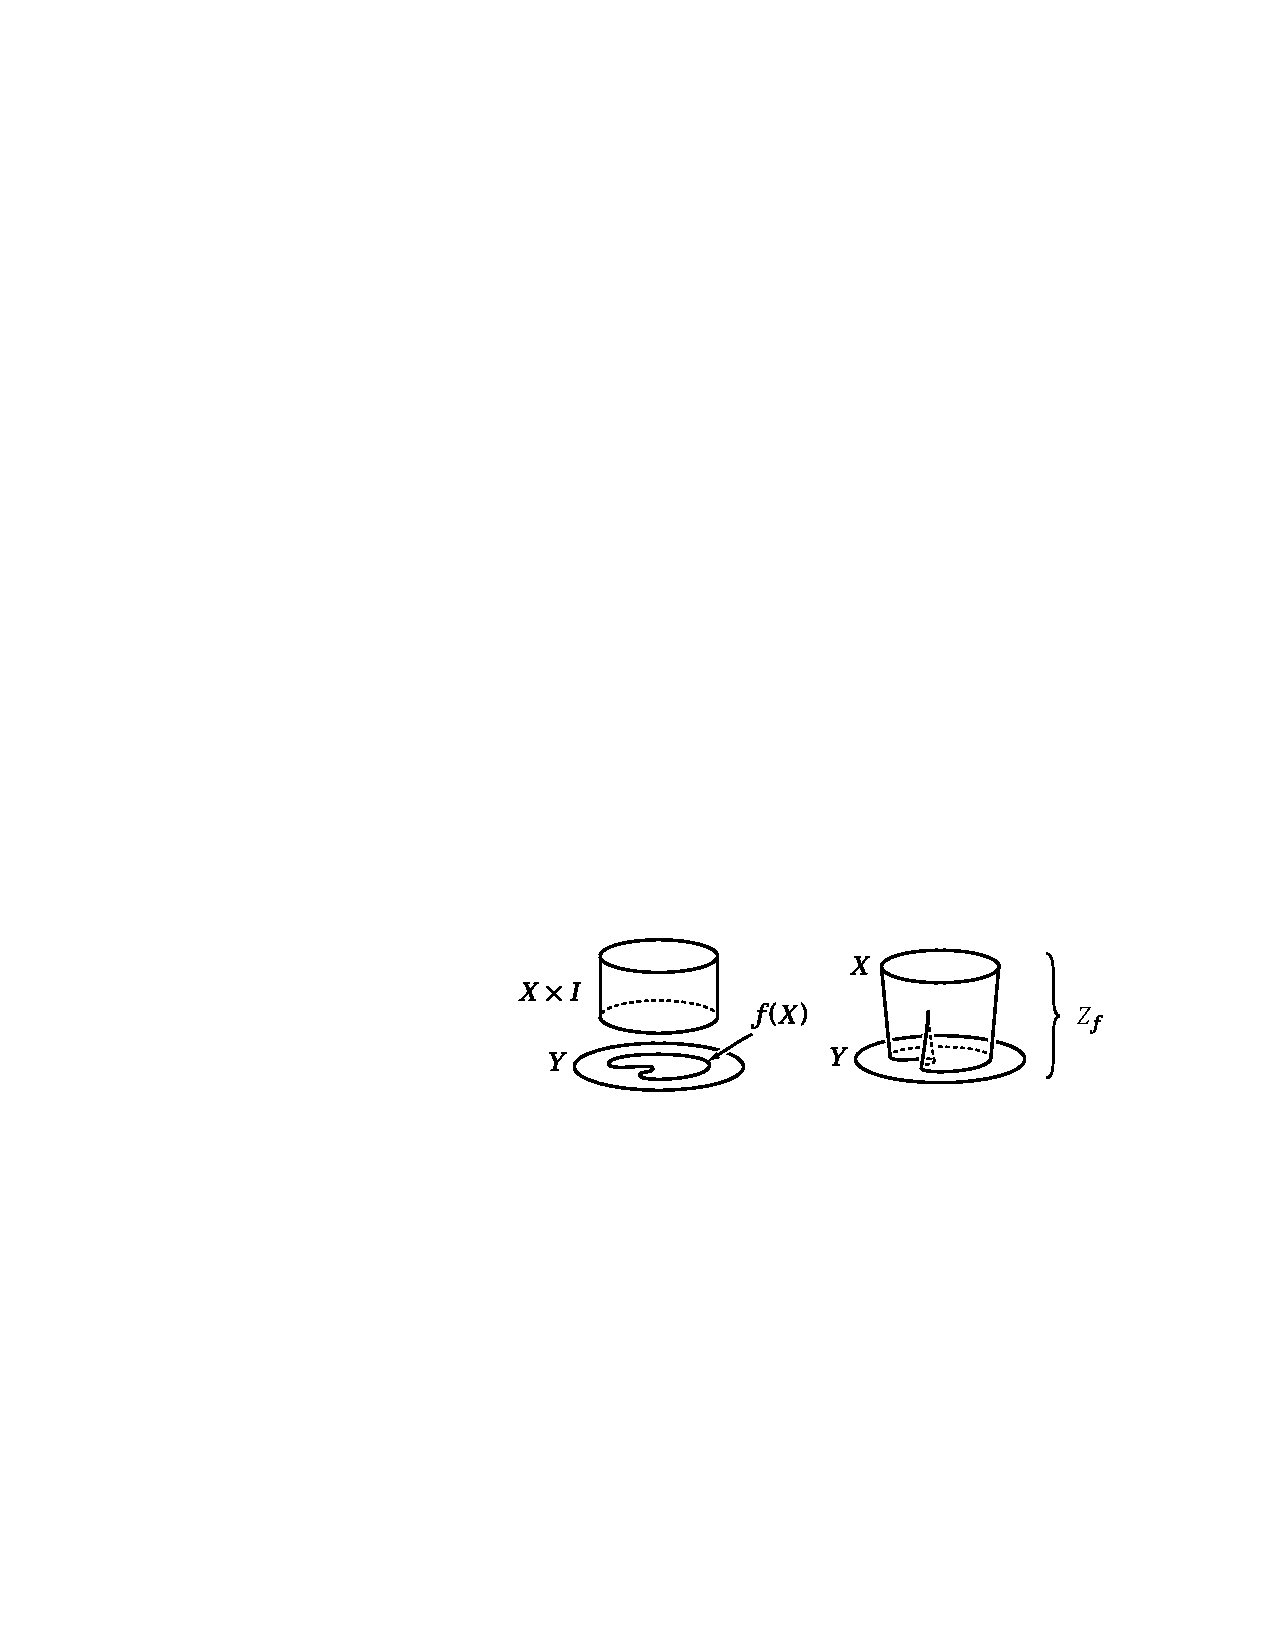
\includegraphics[width=0.5\textwidth]{figures/cylinder.pdf}
    \caption{Mapping cylinder of $f$.}
    \label{fig:mapping cyl}
\end{figure}

\begin{defn}[Mapping cylinder]\index{Mapping cylinder}
    Let $f:X\to Y$ be a map. The mapping cylinder of $f$ is the pushout $Z_f$, see Figure~\ref{fig:mapping cyl}, defined as the quotient of $(X\times I)\sqcup Y$ that identifies $(x,0)\in X\times I$ with $f(x)\in Y$:
    \[
    \begin{tikzcd}[every matrix/.append style={name=m}, row sep=large, column sep=large]
       X \sqcup X\arrow[r,"f\sqcup \mathrm{id}"]\arrow[d,"i_0\sqcup i_1",swap] & Y\sqcup X\arrow[d,"s\sqcup j"]\\
       X\times I \arrow[r,"a", swap] & Z_f
    \end{tikzcd}, \;
    \begin{matrix}
        Z_f=\bigslant{(X\times I)\sqcup Y}{(x,0)\sim f(x)},\\
        s(y)=y,\; j(x)=(x,1), \\ i_0(x)=(x,0),\; i_1(x)=(x,1).
    \end{matrix}
    \]
    We also have the projection $q:Z_f\to Y$, $(x,t)\mapsto f(x)$, $y\mapsto y$.
\end{defn}

The images $q(X\times\{1\})$ and $q(Y)$ are homeomorphic to $X$ and $Y$ respectively. When $X$ and $Y$ are homotopy equivalent, both of these subspaces of $Z_f$ can be shown to be deformation retracts of $Z_f$. Therefore two spaces $X,Y$ are homotopy equivalent iff they are homeomorphic to deformation retracts of some third space $Z$. See, e.g., \cite[Prop.~7.46]{LeeTop} for a proof. We will also provide a proof in Corollary~\ref{cor 0.21 Hatcher}.


\begin{figure}
    \centering
    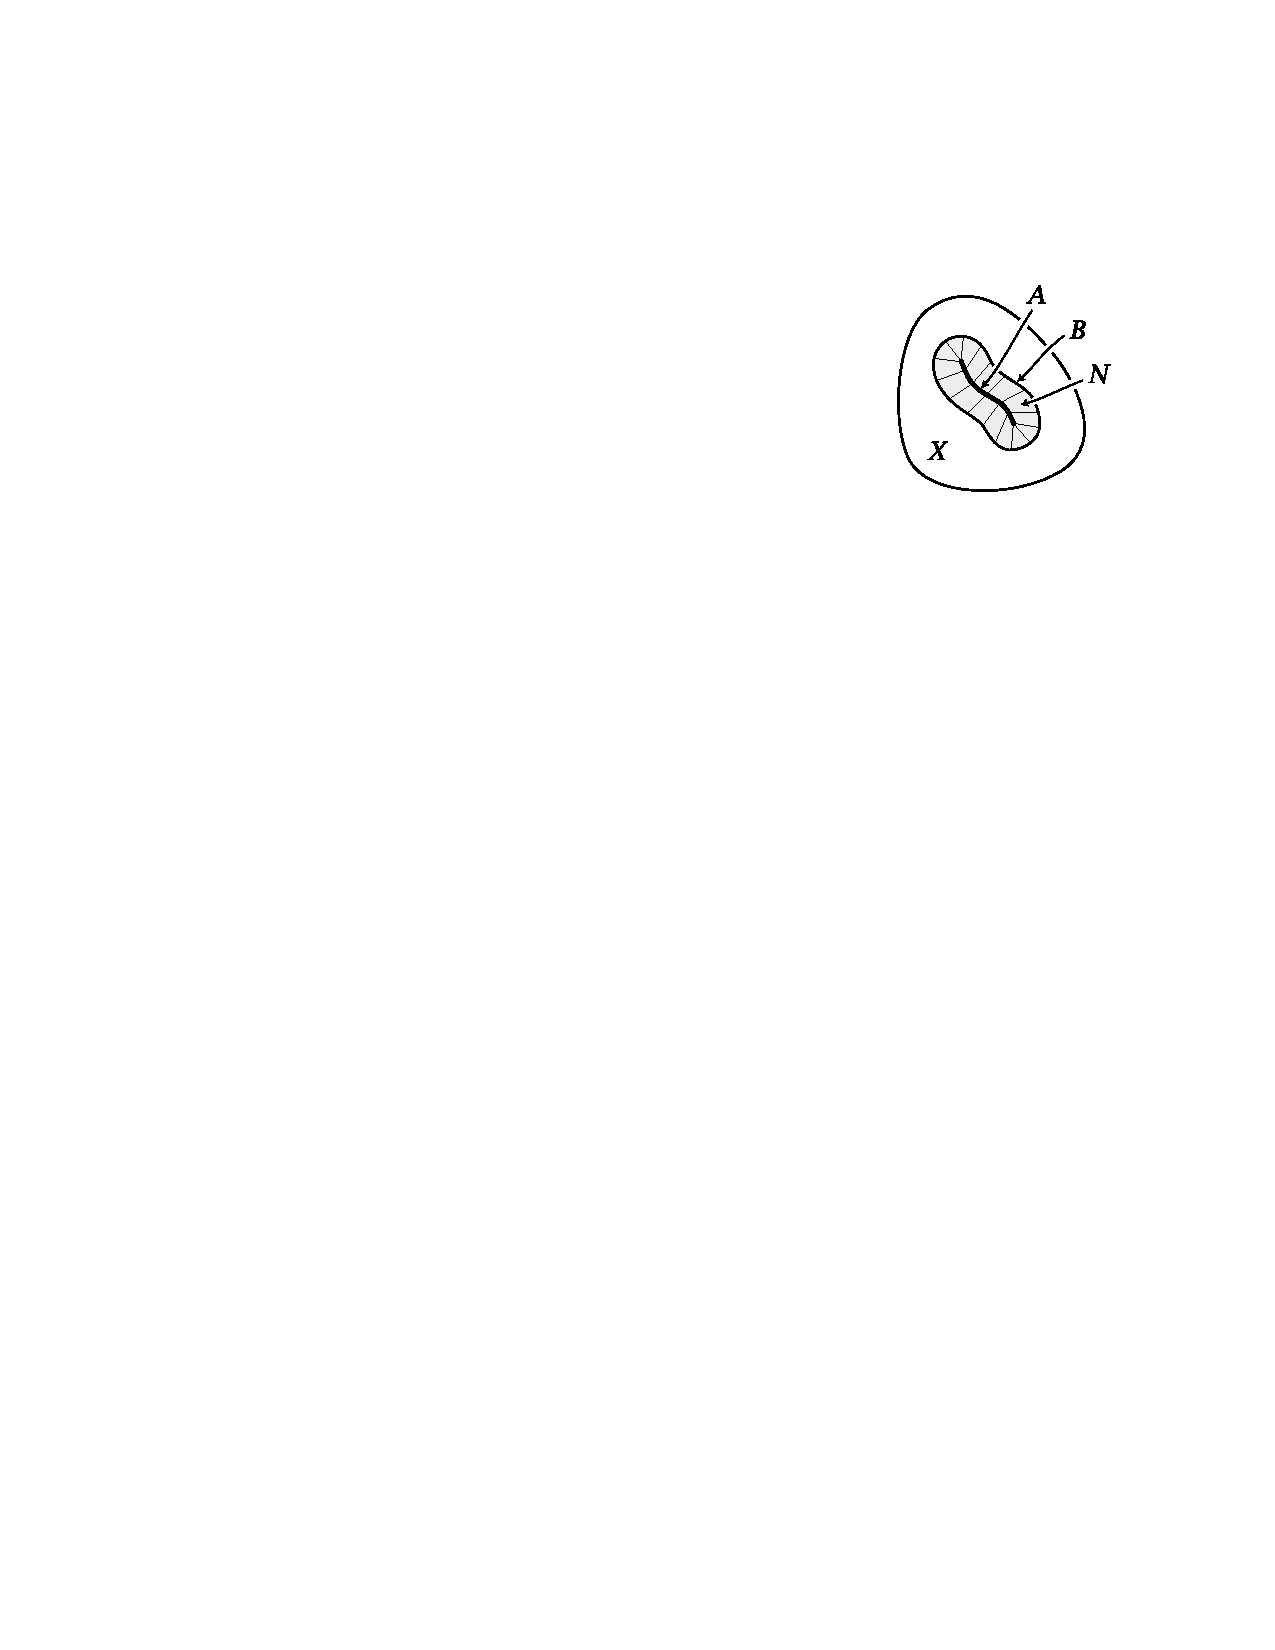
\includegraphics[width=0.3\textwidth]{figures/hep_example.pdf}
    \caption{Mapping cylinder neighborhood from Example~\ref{example Z_f hep}.}
    \label{fig: Z_f hep}
\end{figure}
\begin{example}\label{example Z_f hep}
    A pair $(X,A)$ has the \gls{hep} if $A$ has a mapping cylinder neighborhood of $X$, by which we mean a closed neighborhood $N$ containing a subspace $B$, thought of as the boundary of $N$, with $N\setminus B$ an open neighborhood of $A$, such that there exists a map $f:B\to A$ and a homeomorphism $h:Z_f\to N$ with $\restr{h}{A\cup B}=\id$. Mapping cylinder neighborhoods like this occur fairly often. For example thickened graphs in the plane, see Figure~\ref{fig: Z_f hep}.
\end{example}

\begin{xca}
    Show that the mapping cylinder of the double covering map $\pi$ of the circle $\bbS^1$ ($\pi(z)=z^2$ on the unit circle in $\bbC$) is homeomorphic to a bounded M\"obius band.
\end{xca}


\begin{prop}[{{\cite[Prop.~0.16]{Hatcher}}}]\label{prop 0.16 Hatcher}
    If $(X,A)$ is a $CW$ pair (i.e.~$A$ is a subcomplex of $X$), then $(X\times\{0\})\cup (A\times I)$ is a deformation retract of $X\times I$, hence $(X,A)$ is a cofibration.
\end{prop}
\begin{proof}
    There is a retraction $r:\bbD^n\times I\to (\bbD^n\times\{0\})\cup (\partial \bbD^n\times I)$, for example the radial projection from the point $(0,2)\in \bbD^n\times \bbR$. Then setting $r_t=t\cdot r+(1-t)\id$ gives a deformation retraction of $\bbD^n\times I$ onto $(\bbD^n\times\{0\})\cup (\partial \bbD^n\times I)$. This deformation gives rise to a deformation retraction of $X^{(n)}\times I$ onto $(X^{(n)}\times\{0\})\cup ((X^{(n-1)}\cup A^{(n)})\times I)$ since $X^{(n)}$ is obtained from the latter by attaching copies of $\bbD^n\times I$ along $(\bbD^n\times\{0\})\cup (\partial \bbD^n\times I)$. If we perform this deformation retraction in dimension $n$ during the $t$-interval $[2^{-n-1},2^{-n}]$, this infinite concatenation of homotopies is a deformation retraction of $X\times I$ onto $(X\times\{0\})\cup (A\times I)$. There is no problem with continuity of this deformation at $t=0$ since it is continuous on $X^{(n)}\times I$, being stationary there during the $t$-interval $[0,2^{-n-1}]$, and $CW$-complexes have the weak topology with respect to their skeleta so a map is continuous iff its restriction to each skeleton is continuous.
\end{proof}

\begin{prop}[{{\cite[Prop.~0.17]{Hatcher}}}]
    If the pair $(X,A)$ is a cofibration and $A$ is contractible, then the quotient map $q:X\to X\slash A$ is a homotopy equivalence.
\end{prop}
\begin{proof}
    We can use the \gls{hep} to extend a contraction of $A$ to a homotopy of maps $X\to X$ that map $A$ to $A$. This descends to a homotopy of maps $X\slash A\to X\slash A$. At $t=1$ this homotopy produces a map that maps $A$ to the point to which $A$ was contracted, so this map induces a map $X\slash A\to X$. It is then easy to see that this map is a homotopy inverse of $q$ via the two homotopies constructed above.
\end{proof}

\begin{prop}[{{\cite[Prop.~0.18]{Hatcher}}}]
    If $(X_1,A)$ is a $CW$-pair and we have the attaching maps $f,g:A\to X_0$ that are homotopic, then $X_0\sqcup_f X_1\simeq X_0\sqcup_g X_1 \rel X_0$.
\end{prop}
\begin{proof}
    If $F:A\times I\to X_0$ is the homotopy from $f$ to $g$, then consider the space $X_0\sqcup_F (X_1\times I)$. This contains both spaces in the claim of the theorem as subspaces. A deformation retraction of $X_1\times I$ onto $(X_1\times \{0\})\cup (A\times I)$ as in Proposition~\ref{prop 0.16 Hatcher} induces a deformation retraction of $X_0\sqcup_F (X_1\times I)$ onto $X_0\sqcup_f X_1$. Similarly that space retracts onto $X_0\sqcup_g X_1$. Both of these deformation retractions restrict to the identity map on $X_0$, so they give the necessary homotopy equivalence.
\end{proof}

\begin{prop}[{{\cite[Prop.~0.19]{Hatcher}}}]
    Suppose $(X,A)$ and $(Y,A)$ are cofibrations and $f:X\to Y$ is a homotopy equivalence with $\restr{f}{A}=\id_A$. Then $f$ is a homotopy equivalence $\rel A$.
\end{prop}
\begin{proof}
    We only outline the proof, see \cite[Prop.~0.19]{Hatcher} for the full details. Let $g:Y\to X$ be a homotopy inverse of $f$. The idea is to construct a homotopy from $g$ to a map $g_1$ such that $\restr{g_1}{A}=\id_A$. This is possible by taking the existing homotopy from $g\circ f$ to $\id_X$, restricting it to a homotopy from $\restr{g}{A}$ to $\id_A$, and extending it to a homotopy of maps $Y\to X$. At $t=1$ this homotopy will give the necessary $g_1$. Then we check that $g_1\circ f\simeq \id_X \,\rel A$ and that $f\circ g_1\simeq \id_Y\,\rel A$.  
\end{proof}
By applying the above to the inclusion map we immediately get the next Corollary.
\begin{cor}[{{\cite[Cor.~0.20]{Hatcher}}}]
    If $(X,A)$ is a cofibration and the inclusion $i:A\hookrightarrow X$ is a homotopy equivalence, then $A$ is a deformation retract of $X$.
\end{cor}
\begin{cor}[{{\cite[Cor.~0.21]{Hatcher}}}]\label{cor 0.21 Hatcher}
    A map $f:X\to Y$ is a homotopy equivalence iff $X$ is a deformation retract of the mapping cylinder $Z_f$. Hence, two spaces $X\simeq Y$ iff there is a third space containing both $X$ and $Y$ as deformation retracts.
\end{cor}
\begin{proof}
    We have the inclusions $i:X\hookrightarrow Z_f$ and $j:Y\hookrightarrow Z_f$, and the canonical retraction $r:Z_f\to Y$, so $f=r\circ i$ and $i\simeq j\circ f$. Since $j$ and $r$ are homotopy equivalences (``h.e.''), it follows that $f$ is a h.e.\ iff $i$ is h.e., since the composition of two h.e.'s\ is a h.e.\ and a map homotopic to a h.e.\ is also a h.e. Now we apply the preceding corollary to the pair $(Z_f,X)$, which is a cofibration by Example~\ref{example Z_f hep} using the neighborhood $X\times [0,\frac12]$ of $X$ in $Z_f$.
\end{proof}





\section{Whitehead's theorem}

Let us first adapt the Compression Criterion (Proposition~\ref{prop: compression criterion}) to the context of $CW$-complexes.

\begin{lem}[Compression Lemma]\index{Lemma!compression}
    Let $(X,A)$ be a $CW$ pair (i.e.~$A$ is a subcomplex of $X$) and let $(Y,B)$ be any pair with $B\neq\varnothing$. For each $n$ such that $X\setminus A$ has cells of dimension $n$, assume that $\pi_n(Y,B,y_0)=0$ for all $y_0\in B$. Then every map $f:(X,A)\to (Y,B)$ is homotopic $\rel A$ to a map $X\to B$.

    When $n=0$ the condition $\pi_n(Y,B,y_0)=0$ for all $y_0\in B$ is to be regarded as saying that $(Y,B)$ is connected.
\end{lem}
\begin{proof}
    Assume inductively that $f$ has already been homotoped to take the skeleton $X^{(k-1)}$ to $B$. If $\Phi$ is the characteristic map of a $k$-cell $e^k$ of $X\setminus A$, the composition $f\circ \Phi:(\bbD^k,\partial \bbD^k)\to (Y,B)$ can be homotoped into $B$ $\rel \partial \bbD^k$ in view of the hypothesis that $\pi_k(Y,B,y_0)=0$ if $k>0$, or that $(Y,B)$ is $0$-connected if $k=0$. This homotopy of $f\circ\Phi$ induces a homotopy of $f$ on the quotient space $X^{(k-1)}\cup e^k$ of $X^{(k-1)}\sqcup \bbD^k$, a homotopy $\rel X^{(k-1)}$. Doing this for all $k$-cells of $X\setminus A$ simultaneously, and taking a constant homotopy on $A$, we obtain a homotopy of $\restr{f}{X^{(k)}\cup A}$ to a map into $B$. By the homotopy extension property, this homotopy extends to a homotopy defined on all of $X$, and the induction step is completed.

    Finitely many applications of the induction step finish the proof if the cells of $X\setminus A$ are bounded in dimension. Otherwise, we can perform the homotopy of the induction step during the $t$-interval $[1-2^{-k},1-2^{-k-1}]$. Any finite skeleton $X^{(k)}$ is eventually stationary under these homotopies, hence we have a well-defined homotopy $f_t$, $t\in [0,1]$ with $f_1(X)\subset B$.
\end{proof}


\begin{thm}[Whitehead's Theorem]\index{Theorem!Whitehead}\label{thm whitehead}
    If a map $f:X\to Y$ between connected $CW$-complexes induces isomorphisms $f_\ast :\pi_n(X)\to \pi_n(Y)$ for all $n$, then $f$ is a homotopy equivalence. 
    
    If $f$ is the inclusion map of a subcomplex $X\hookrightarrow Y$, the conclusion is stronger: $X$ is a deformation retract of $Y$.
\end{thm}
\begin{proof}
    In the special case that $f$ is the inclusion of a subcomplex, consider the long exact sequence on all homotopy groups of $(Y,X)$. Since $f$ induces isomorphisms of all homotopy groups, the relative groups $\pi_n(Y,X)$ are zero. Applying the Compression Lemma to the identity map on $(Y,X)$ then yields a deformation retraction of $Y$ onto $X$.

    The general case can be proved using mapping cylinders. Recall that the mapping cylinder $Z_f$ is the quotient space of the disjoint union of $X\times I$ and $Y$ under the identifications $( x, 1 ) \sim f ( x )$. Thus $Z_f$ contains both $X = X\times { 0 }$ and $Y$ as subspaces, and $Z_f$ deformation retracts onto $Y$. The map $f$ becomes the composition of the inclusion $X\hookrightarrow Z_f$ with the retraction $Z_f\to Y$. Since this retraction is a homotopy equivalence, it suffices to show that $Z_f$ deformation retracts onto $X$ if $f$ induces isomorphisms on homotopy groups, or equivalently, if the relative groups $\pi_n(Z_f,X)$ are all trivial.

    If the map $f$ happens to be \emph{cellular}\index{Cellular map}, i.e.~taking $X^{(n)}$ to $Y^{(n)}$, then $(Z_f,X)$ is a $CW$-pair and so we are done by the first paragraph of the proof. If $f$ is not cellular, we can either appeal to the Cellular Approximation Theorem~\ref{thm cell approx} which says that $f$ is homotopic to a cellular map, or use the following argument. First apply the Compression Lemma to obtain a homotopy $\rel X$ of the inclusion $(X\cup Y,X)\hookrightarrow (Z_f,X)$ to a map into $X$. Since the pair $(Z_f,X\cup Y)$ obviously is a cofibration, this homotopy extends to a homotopy from $\id_{Z_f}$ to a map $g:Z_f\to Z_f$ taking $X\cup Y$ into $X$. Then apply the Compression Lemma again to the composition $((X\times I)\sqcup Y,(X\times\partial I)\sqcup Y)\to (Z_f,X\cup Y)\overset{g}{\to} (Z_f,X)$ to finish the construction of a deformation retraction of $Z_f$ onto $X$.
\end{proof}

\begin{rem}
    The Whitehead theorem \emph{does not} say that two complexes with isomorphic homotopy groups are homotopy equivalent -- the existence of a map $f$ that generates those isomorphisms is crucial! For example, $\RP^2$ and $\bbS^2\times \RP^\infty$ both have fundamental group $\bbZ_2$ and trivial higher groups (since their universal covers $\bbS^2$ and $\bbS^2\times \bbS^\infty$ are homotopy equivalent,  $\bbS^\infty$ being contractible). But these two spaces are not homotopy equivalent because they have vastly different homology groups.
\end{rem}

\begin{defn}[Weak homotopy equivalence]
    A map $f:X\to Y$ is called a weak homotopy equivalence if all the induced homomorphisms $f_\ast:\pi_n(X,*)\to \pi_n(Y,*)$, $n\geq 0$, are isomorphisms regardless of the choice of basepoints.
\end{defn}


Whitehead's theorem therefore states that a weak homotopy equivalence between $CW$-complexes is actually a homotopy equivalence.  In general, however, weak homotopy equivalences are a much bigger class of maps. For example, there exist noncontractible spaces whose homotopy groups are all trivial, such as the `quasi-circle'. For such spaces a map to a point is a weak homotopy equivalence that but not a homotopy equivalence. 

One special case where isomorphisms by themselves do imply homotopy equivalence is when all homotopy groups are trivial.

\begin{defn}[Weakly contractible space]\index{Weakly contractible space}
    A space $X$ is called weakly contractible if $\pi_n(X)$ is trivial for all $n\geq 0$.
\end{defn}

\begin{cor}
    A weakly contractible $CW$-complex is contractible.
\end{cor}
\begin{proof}
    The inclusion map of a $0$-cell into the complex induces an isomorphism of the trivial homotopy groups, therefore by Whitehead's theorem there is a homotopy equivalence with a point.
\end{proof}

\begin{lem}[Extension Lemma]\label{lem 4.7 Hatcher}
    Let $(X,A)$ be a $CW$-pair and $Y$ is a path-connected space such that $\pi_{n-1}(Y)=0$ for all $n$ in which $X^{(n)}\setminus A^{(n)}\neq \varnothing$. Then any continuous map $f:A\to Y$ can be extended to a map $\wt f:X\to Y$.
\end{lem}
\begin{proof}
    Assume $f$ was already extended to a map $f^{(n-1)}$ over the $(n-1)$-skeleton. Then an extension over all $n$-cells exists iff the composition of the cell's attaching map $\bbS^{n-1}\to X^{(n-1)}$ with $f^{(n-1)}$ is nullhomotopic.
\end{proof}





\section{Cellular approximation}


Recall when we applied the van Kampen theorem to compute $\pi_1(\bbS^n)=0$ for $n\geq 2$, we implicitly used the fact that every loop can be deformed to miss at least one point in $\bbS^n$, and then it can obviously be contracted to a point since $\bbS^n\setminus *$ is contractible. This is not an obvious fact since there exist space-filling loops that are surjective. Similar space-filling maps exist for all pairs $\bbS^m\to \bbS^n$ with $m<n$.

For homotopy theory of $CW$ complexes it turns out to be sufficient to work with maps that map $n$-skeleta to $n$-skeleta, and any other map is homotopic to one of this class.



\begin{lem}[{{\cite[Lem.~4.10]{Hatcher}}}]\label{lem 4.10 hatcher}
    Let $f:Y^n\to Z$ be a map, where $Z$ is obtained from a subspace $W$ by attaching a $k$-cell $e^k$. Then there is a homotopy $f_t:(I^n,f^{-1}(e^k))\to (Z,e^k)$ $\rel f^{-1}(W)$ from $f=f_0$ to a map $f_1$ for which there is a polyhedron $K\subset I^n$ such that:
    \begin{enumerate}[label=(\alph*)]
        \item $f_1(K)\subset e^k$ and $\restr{f_1}{K}$ is piecewise linear (i.e.~linear on each face of $K$) with respect to some identification of $e^k$ with $\bbR^n$.
        \item There exists a nonempty open $U\subset e^k$ such that $f_1^{-1}(U)\subset K$.
    \end{enumerate}
\end{lem}
\begin{proof}
    Identifying $e^k$ with $\bbR^k$, let $B_1,b_2\subset e^k$ be the closed balls of radius $1$ and $2$ at the origin. Since $f^{-1}(B_2)$ is closed and therefore compact in $I^n$, it follows that $f$ is uniformly continuous on $f^{-1}(B_2)$. Thus there exists $\epsilon>0$ such that $|x-y|<\epsilon$ implies $|f(x)-f(y)|<\frac 12$ for all $x,y\in f^{-1}(B_2)$. Subdivide the interval $I$ so that the induced subdivision of $I^n$ into cubes has each cube lying in a ball of diameter less than $\epsilon$. Let $K_1$ be the union of all the cubes meeting $f^{-1}(B_1)$ and let $K_2$ be the union of all cubes meeting $K_1$. We may assume $\epsilon$ is chosen smaller than half the distance between the compact sets $f^{-1}(B_1)$ and $I^n\setminus f^{-1}(\int B_2)$, and then we will have $K_2\subset f^{-1}(B_2)$. See Figure~\ref{fig:cell_approx}.

    Now we subdivide all the cubes of $K_2$ into simplices. This can be done inductively in the dimension by taking the center point of a cube as a new vertex and joining it by a cone to each simplex in boundary of the cube. 

    Let $g:K_2\to e^k=\bbR^k$ be the map that equals $f$ on all vertices of simplices of the subdivision and is linear on each simplex. Let $\varphi:K_2\to [0,1]$ be the map that is linear on simplices and has value $1$ on vertices in $K_1$ and $0$ on vertices of $K_2\setminus K_1$. Thus $\restr{\varphi}{K_1}=1$. Define a homotopy $f_t:K_2\to e^k$ by the formula $(1-t\varphi)\cdot f+(t\varphi)\cdot g$, so $f_0=f$ and $\restr{f_1}{K_1}=\restr{g}{K_1}$. Since $f_t$ is constant in $t$ on simplices in $K_2$ disjoint from $K_1$, and in particular on simplices in the closure $\widebar{I^n\setminus K_2}$, we may extend $f_t$ to be the constant homotopy of $f$ on $I^n\setminus K_2$.

    The map $f_1$ takes the closure $\widebar{I^n\setminus K_1}$ to a compact set $C$ which, we claim, is disjoint from the center $0$ of $B_1$ and hence from a neighborhood $U$ of $0$. This will prove the lemma, with $K=K_1$ since we will have $f_1^{-1}(U)\subset K_1$ with $f_1$ piecewise linear on $K_1$ where it is equal to $g$.

    The verification of the claim has two steps:
    \begin{enumerate}[label=(\arabic*)]
        \item On $I^n\setminus K_2$ we have $f_1=f$, and $f$ takes $I^n\setminus K_2$ outside $B_1$ since $f^{-1}(B)\subset K_2$ by construction.
        \item For a simplex $\sigma$ of $K_2$ not in $K_1$ we have $f(\sigma)$ contained in some ball $B_\sigma$ of radius $\frac 12$ by the choice of $\epsilon$ and the fact that $K_2\subset f^{-1}(B_2)$. Since $B_\sigma$ is convex, we must also have $g(\sigma)\subset B_\sigma$. We know that $g(\sigma)\subset B_\sigma$, hence also $f_t(\sigma)\subset B_\sigma$ for all $t$, and in particular $f_1(\sigma)\subset B_\sigma$. We know that $B_\sigma\cancel{\subset} B_1$ since $\sigma\cancel{\subset}K_1$ and thus $\sigma\cancel{\subset}f^{-1}(B_1)$. The radius of $B_\sigma$ is half that of $B_1$, so it follows that $0\notin B_\sigma$, and hence $0\notin f_1(\sigma)$.
    \end{enumerate}
\end{proof}

\begin{figure}
    \centering
    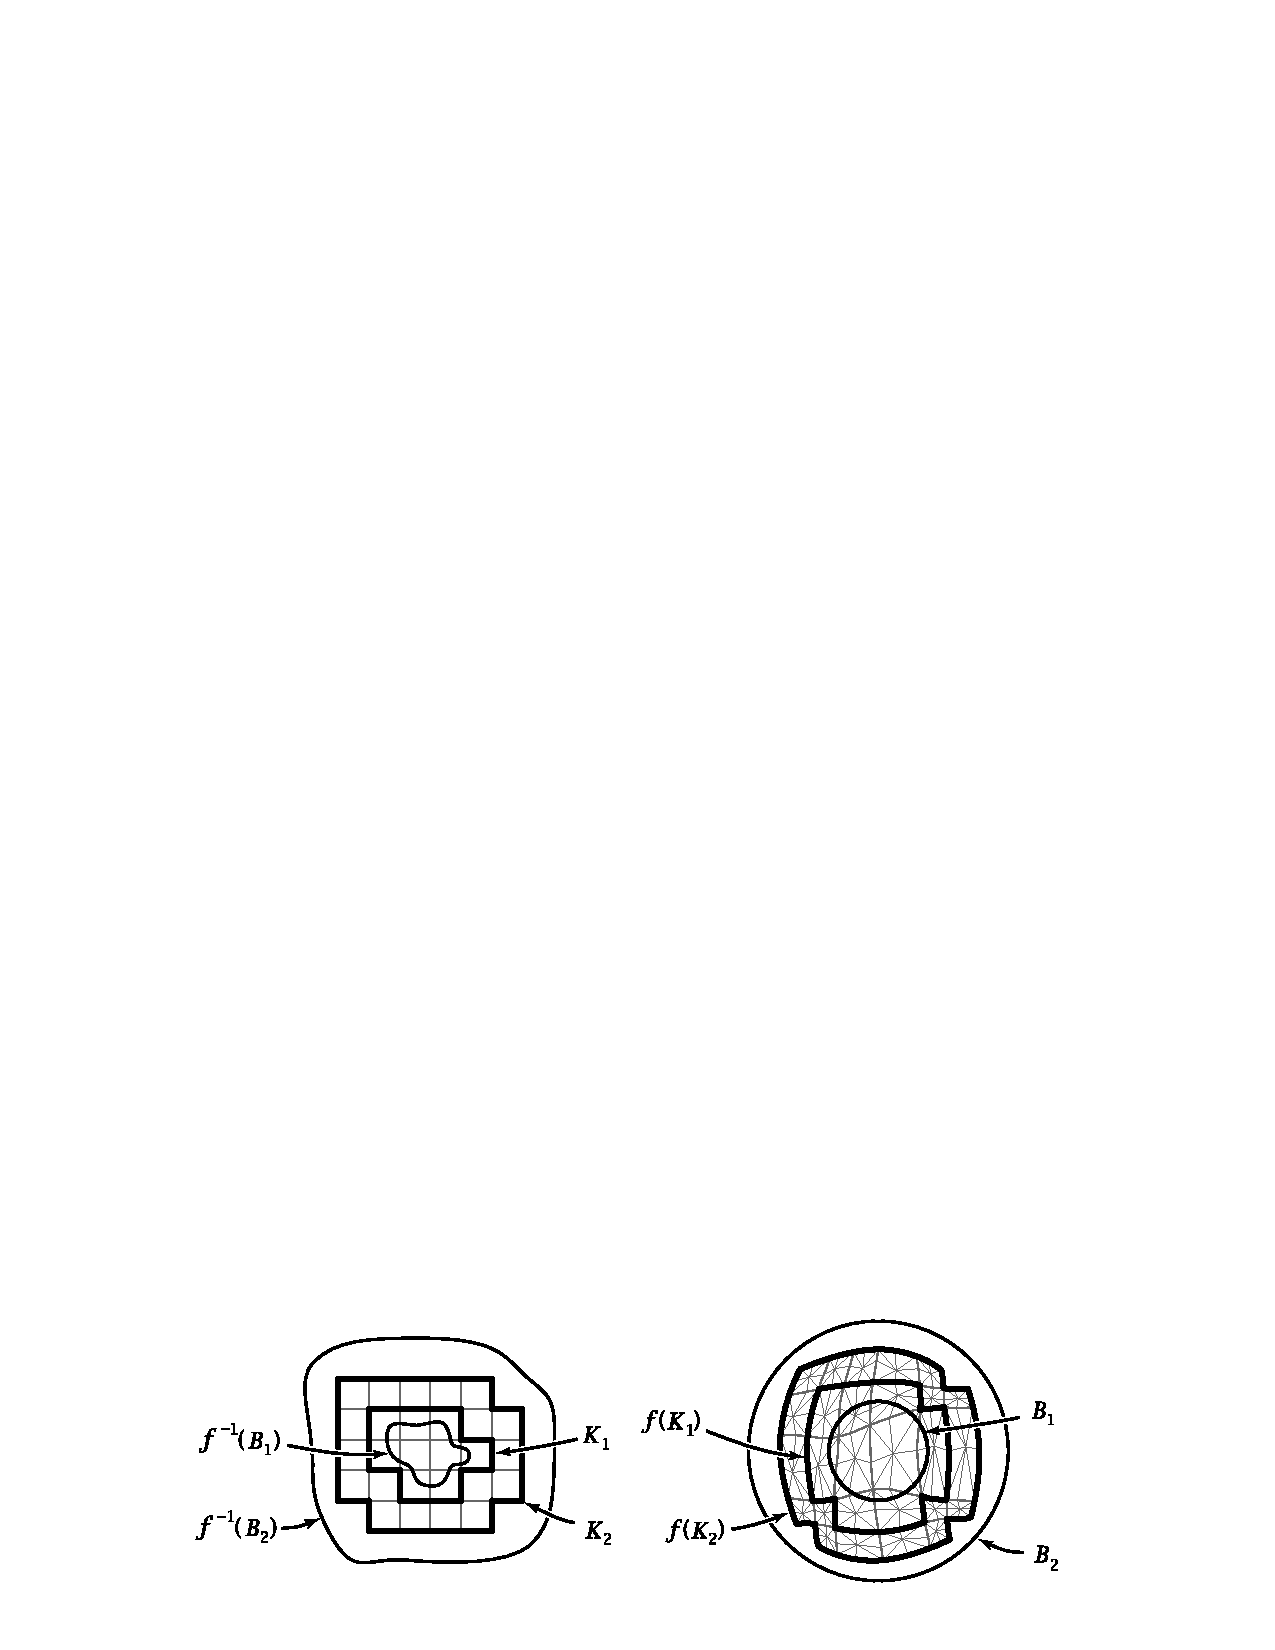
\includegraphics[width=0.7\textwidth]{figures/cell_approx.pdf}
    \caption{Subdivision from the proof of Lemma~\ref{lem 4.10 hatcher}.}
    \label{fig:cell_approx}
\end{figure}


\begin{thm}[Cellular Approximation Theorem]\index{Theorem!Cellular Approximation}\label{thm cell approx}
    Every map $f:X\to Y$ of $CW$-complexes is homotopic to a cellular map. 

    Every map $f:(X,A)\to (Y,B)$ of $CW$-pairs is homotopic $\rel A$ to a cellular map.
\end{thm}
\begin{proof}
    Suppose inductively that $f$ is cellular on $X^{(n-1)}$, and let $e^n$ be an $n$-cell of $X$. The closure of $e^n$ in $X$ is compact, being the image of a characteristic map for $e^n$ (Proposition~\ref{prop f(compact)=compact}), so $f$ takes the closure of $e^n$ to a compact set in $Y$.  Therefore $f(e^n)$ meets finitely many cells of $Y$.  Let $e^k\subset Y$ be a cell of highest dimension meeting $f(e^n)$. We may assume $k>n$, otherwise $f$ is already cellular on $e^n$.

    Now we apply Lemma~\ref{lem 4.10 hatcher} to the composition of $f:X^{(n-1)}\cup e^n\to Y^{(k)}$ with a characteristic map $I^n\to X$ for $e^n$, with $Z=Y^{(k)}$ and $W=Y^{(k)}\setminus e^k$. The homotopy given by the lemma is fixed on $\partial I^n$, hence induces a homotopy $f_t$ of $\restr{f}{X^{(n-1)}\cup e^n}$ fixed on $X^{(n-1)}$. The image of the resulting map $f_1$ intersects the open set $U\subset e^k$ in a set contained in the union of finitely many hyperplanes of dimension at most $n$, so if $n<k$ there will be points $p\in U$ not in the image of $f_1$. 
    
    In summary, it is possible to deform $\restr{f}{X^{(n-1)}\cup e^n}$, staying fixed on $X^{(n-1)}$, so that $f(e^n)$ misses some point $p\in e^k$. Then we can deform $\restr{f}{X^{(n-1)}\cup e^n}$ $\rel X^{(n-1)}$ so that $f(e^n)$ misses the whole cell $e^k$ by composing with a deformation retraction of $Y^{(k)}\setminus \{p\}$ onto $Y^{(k)}\setminus e^k$. By finitely many iterations of this process we eventually make $f(e^k)$ miss all cells of dimension greater than $n$. Doing this for all $n$-cells simultaneously, staying fixed on $n$-cells in $A$ where $f$ is already cellular, we obtain a homotopy of $\restr{f}{X^{(n)}}$ $\rel X^{(n-1)}\cup A^{(n)}$ to a cellular map. 

    The induction step is then completed by appealing to the \gls{hep} in Proposition~\ref{prop 0.16 Hatcher} to extend this homotopy, together with the constant homotopy on $A$, to a homotopy defined on all of $X$. Letting $n$ go to infinity, the resulting possibly infinite sequence of homotopies can be realized as a single homotopy by performing the $n$-th homotopy during the $t$-interval $[1-2^{-n},1-2^{-n-1}]$. This homotopy will eventually be stationary on every $k$-skeleton and hence continuous at $1$.
\end{proof}

\begin{cor}\label{cor pi_n(S^k)=0}
    $\pi_n(\bbS^k)=0$ for $n<k$.
\end{cor}
\begin{proof}
    If $\bbS^n$ and $\bbS^k$ are given $CW$ structures with one $0$-cell (serving as as basepoint) and one $n(k)$-cell, then every pointed map $\bbS^n\to \bbS^k$ can be homotoped, fixing the basepoint, to be cellular, and hence constant if $n<k$.
\end{proof}





\section{\texorpdfstring{$CW$}{CW} approximation}\label{sec: CW approx}

Whitehead's theorem obviously holds not just for $CW$-complexes, but also for spaces that are homotopy equivalent to them. We now show that any topological space is \emph{weakly} homotopy equivalent to a $CW$-complex.

\begin{defn}[$CW$ approximation]
    A $CW$ approximation of a topological space $X$ is a $CW$-complex $Z$ with a weak homotopy equivalence $f:Z\to X$.
\end{defn}

\begin{prop}[{{\cite[Prop.~4.13]{Hatcher}}}]
    Every space $X$ has a $CW$ approximation $f:Z\to X$. If $X$ is path-connected, $Z$ can be chosen to have a single $0$-cell, with all other cells attached by pointed maps. Thus every connected $CW$-complex is homotopy equivalent to a $CW$-complex with these additional properties.
\end{prop}
\begin{proof}
    The construction of a $CW$ approximation $f:Z\to X$ for a space $X$ is inductive. Suppose given a $CW$-complex $A$ with a map $f:A\to X$ and suppose we have chosen a basepoint $0$-cell $*$ in each component of $A$. Then for an integer $k\geq 0$ we will attach $k$-cells to $A$ to form a $CW$ complex $B$ with a map $f:B\to X$ extending the given $f$, such that the induced homomorphism $f_\ast:\pi_i(B,*)\to \pi_i(X,f(*))$ is injective for $i=k-1$ and surjective for $i=k$, for all basepoints $*$.

    There are two steps:
    \begin{enumerate}[label=(\arabic*)]
        \item Choose maps $\varphi_\alpha:(\bbS^{k-1},s_0)\to (A,*)$ representing a set of generators for the kernel of $f_\ast:\pi_{k-1}(A,*)\to \pi_{k-1}(X,f(*))$ for all basepoints $*$. We map assume the maps $\varphi_\alpha$ are cellular, where $\bbS^{k-1}$ has its standard $CW$ structure with $s_0$ as the $0$-cell. Attaching cells $e_\alpha^k$ to $A$ via $\varphi_\alpha$ then produces a $CW$ complex, and the map $f$ extends over these cells using nullhomotopies of $f\circ \varphi_\alpha$, which exist by the choice of the $\varphi_\alpha$'s.
        \item Choose maps $f_\beta:\bbS^k\to X$ representing generators for the groups $\pi_k(X,f(*))$, attach cells $e_\beta^k$ to $A$ via the constant maps at the appropriate basepoints $*$, and extend $f$ over the resulting spheres $S_\beta^k$ via the $f_\beta$'s.
    \end{enumerate}

    The surjectivity of $f_\ast$ holds by construction. For the injectivity, an element of the kernel of $f_\ast:\pi_{k-1}(B,*)\to \pi_{k-1}(X,f(*))$ can be represented by a cellular map $h:\bbS^{k-1}\to B$. This has image in $A$, so is in the kernel of $f_\ast:\pi_{k-1}(A,*)\to \pi_{k-1}(X,f(*))$ and hence is homotopic to a linear combination of the $\varphi_\alpha$'s, which are nullhomotopic in $B$, so $h$ is nullhomotopic as well. When $k=1$ there is no group structure on $\pi_{k-1}$ so injectivity on $\pi_0$ does not follow from having a trivial kernel, and we modify the construction by choosing the cells $e_\alpha^1$ to join each pair of basepoints $*$ that map by $f$ to the same path-component of $X$. The map $f$ can then be extended over these $1$-cells $e_\alpha^1$.

    Note that if $f$ happened to be injective or surjective on $\pi_i$ for some $i<k-1$ or $i<k$, respectively, then this remains true after attaching the $k$-cells. This is because attaching $k$-cells does not affect $\pi_i$ if $i<k-1$, by cellular approximation, not does it destroy surjectivity on $\pi_{k-1}$ or indeed any $\pi_i$, obviously.

    Now to construct a $CW$ approximation $f:Z\to X$ one can start with $A$ consisting of one point for each path-component of $X$, with $f:A\to X$ mapping each of them to the corresponding path-component. Having now a bijection on $\pi_0$, attach $1$-cells to $A$ to create a surjection on $\pi_1$  for each path-component, then $2$-cells to improve this to an isomorphism on $\pi_1$ and a surjection on $\pi_2$, and so on for each successive $\pi_i$. After all cells have been attached one has a $CW$-complex $Z$ and a weak homotopy equivalence $f:Z\to X$.
\end{proof}

\begin{rem}
    One can apply this technique to produce $CW$ approximations of pairs $(X,A)$. First construct a $CW$ approximation $f_A:Z_A\to A$, then starting with the composition $Z_A\to A\hookrightarrow X$, attach cells to $Z_A$ to create a weak homotopy equivalence $f:Z\to X$ extending $f_A$. The induced map $f_\ast$ will be an isomorphism of relative homotopy groups  by the five-lemma~\ref{5-lemma} applied to the two sequences of morphisms in relative and absolute homotopy.
\end{rem}


Running ahead, we will be calling a $CW$-pair $(Z,A)$ \emph{$n$-connected} if $\pi_k(Z,A,a)=0$ for $k=1,\ldots n$ and all $a\in A$, and the inclusion-induced map $\pi_0(A)\to \pi_0(Z)$ is surjective. 

\begin{defn}[$n$-connected $CW$ model]
    An $n$-connected $CW$ model for a $CW$ pair $(X,A)$ with a nonempty subcomplex $A$ is an $n$-connected $CW$ pair $(Z,A)$ and a map $f:Z\to X$ with $\restr{f}{A}=\id_A$ such that the induced homomorphism $f_\ast:\pi_i(Z)\to \pi_i(X)$ is an isomorphism for $i>n$ and an injection for $i=n$, for all choices of basepoint.
\end{defn}

One can think of $Z$ as a homotopy-theoretic hybrid of $X$ and $A$. As $n$ increases it looks more and more like $A$, and less like $X$. We have just shown that $n$-connected models always exist, and can be obtained from $A$ by attaching cells in dimensions $>n$ so that by cellular approximation $(Z,A)$ is $n$-connected. Moreover, it is not difficult to show (\cite[Prop.~4.18, Cor.~4.19]{Hatcher}) that these models (and therefore $CW$ approximations as well) are unique up to homotopy equivalence $\rel A$. In particular, $CW$ approximations are unique up to homotopy equivalence.



\begin{example}[Postnikov towers]
    We can use this technique to construct, for each connected $CW$-complex $X$, and each $n\geq 1$, a $CW$-complex $X_n$ containing $X$ as a subcomplex such that:
    \begin{enumerate}[label=(\alph*)]
        \item $\pi_i(X_n)=0$ for $i>n$;
        \item The inclusion $X\hookrightarrow X_n$ induces an isomorphism on $\pi_i$ for $i\leq n$.
    \end{enumerate}
    To do this, apply the general construction to the constant map of $X$ to a point, starting at the stage of attaching cells of dimension $n+2$. Thus we attach $(n+2)$-cells to $X$ using cellular maps $\bbS^{n+1}\to X$ that generate $\pi_{n+1}(X)$ to form a space with trivial $\pi_{n+1}$, then for this space we attach $(n+3)$-cells to make $\pi_{n+2}$ trivial, and so on. The result is a complex $X_n$ with the desired properties.

    The inclusion $X\hookrightarrow X_n$ extends to a map $X_{n+1}\to X_n$ since $X_{n+1}$ is obtained from $X$ by attaching cells of dimension at least $n+3$, and $\pi_i(X_n)=0$ for $i>n$ so we can apply the Extension Lemma~\ref{extension lemma}. Thus we have a commutative diagram called a Postnikov tower for X. One can regard the spaces $X_n$ as truncations of $X$ which provide successively better approximations to $X$ as $n$ increases. There is a weak homotopy equivalence between $X$ and the inverse limit of the Postnikov tower $\limit X_n$, i.e.~$X$ is a $CW$ approximation of $\limit X_n$.
    \[
    \begin{tikzcd}[every matrix/.append style={name=m}]
       & \vdots \arrow[d]\\
       & X_3 \arrow[d]\\
       & X_2 \arrow[d]\\
       X\arrow[r]\arrow[ur]\arrow[uur] & X_1
    \end{tikzcd}
    \]
\end{example}


Now we prove one of the statements announced in Remark~\ref{rem: classifying space for discrete G}. 
\begin{prop}\label{prop X_G}
    For every (discrete) group $G$ there exists a path-connected two-dimensional $CW$-complex $X_G$ such that $\pi_1(X_G)\cong G$.
\end{prop}
\begin{proof}
    Consider a presentation of the group as the quotient of a free group $\<J\>$ by some normal subgroup $\<R\>$ generated by a set of relations $R$. Construct the 1-skeleton $X^{(1)}$ of $X_G$ as a wedge sum of circles $\bigvee_{j\in J}\bbS^1$. Every relation describes a loop in $X^{(1)}$: for example if $ab^{-1}c^2$ is a relation, then the loop is given by going around $a$ once, around $b$ once in the opposite direction, and then twice around $c$. For each relation $r\in R$ take a 2-cell $\bbD^2$ with boundary $\bbS^{1}$ and define an attaching map $\varphi_r:\bbS^1\to X^{(1)}$ so that it represents the loop specified by $r$. The resulting $CW$-complex $X_G=X^{(2)}_G$ is then a 2-dimensional complex whose fundamental group is, by construction, isomorphic to $G$.
\end{proof}
We will eventually incorporate this space $X_G$ as into the so called classifying space $\rmB G$, so $\pi_1(\rmB G)\cong \pi_1(X_G)\cong G$, i.e., the inclusion is a weak 1-equivalence. The classifying space $\rmB G$ must have $\pi_{n+1}(\rmB G)\cong \pi_{n}(G)$, so in the case of discrete $G$ this is $\pi_{\geq 2}(\rmB G)\cong 0$. In other words, $\rmB G$ for discrete groups is the first Postnikov truncation of the space $X_G$ we just constructed.


\begin{example}\index{Lens spaces}
    Consider the cyclic group $G=C_n\cong \bbZ\slash n\bbZ$ for some integer $n$. Then $X_G$ is $\RP^2$ for $n=2$, and for higher $n$ it is a subcomplex of the lens space with fundamental group $C_n$.
\end{example}

\begin{defn}[Aspherical space]\index{Aspherical space}
    A space $X$ is called aspherical if $\pi_n(X)=0$ for all $n\geq 2$.
\end{defn}

\begin{defn}[First Eilenberg-MacLane space]\index{Eilenberg-MacLane space}\label{def: K(G,1)}
    For a group $G$, the first Eilenberg-MacLane space for $G$, denoted $\rmK(G,1)$, is defined up to weak homotopy equivalence as an aspherical space whose fundamental group is $G$. It can be realized as the first Postnikov truncation $(X_G)_1$ of the space $X_G$ constructed in Proposition~\ref{prop X_G}, and in the case of discrete $G$ it coincides with the so called classifying space $\rmB G$. Since $\pi_1$ is the only nontrivial homotopy group of $\rmK(G,1)$, its universal covering space is contractible by Whitehead's theorem.
\end{defn}


\begin{rem}
    We will later be able to define Eilenberg-MacLane and classifying spaces so that they are unique up to homotopy equivalence, not just weak homotopy equivalence. Namely they will be required to be quotients of weakly contractible $CW$-complexes by a free group action, and of course weakly contractible $CW$-complexes are actually contractible by Whitehead's theorem, which will induce a homotopy equivalence between the resulting quotients as well.
\end{rem}


\begin{cor}
    For every discrete group $G$ there exists a (unique up to homotopy equivalence) universal $G$-principal covering $\rmE G\to \rmK(G,1)$ with contractible total space $\rmE G$.
\end{cor}

\begin{example}[Lens spaces {{\cite[Example~2.43]{Hatcher}}}]\index{Lens spaces}\label{example Lens spaces}
    Given an integer $m>1$ and integers $l_1,\ldots,l_n$ relatively prime to $m$, define the lens space $L=L_m(l_1,\ldots,l_n)$ as the orbit space $\bbS^{2n-1}\slash \bbZ_m$ of the unit sphere $\bbS^{2n-1}\subset\bbC^n$ with the action of $\bbZ_m$ generated by the rotation $(z_1,\ldots,z_n)\mapsto (e^{2\pi\rmi l_1/m}z_1,\ldots e^{2\pi\rmi l_n/m} z_n)$. In particular, when $m=2$, for any odd $l_i$'s this is the antipodal map and $L=L_2(1,\ldots,1)=\RP^{2n-1}$. In general, the projection $\bbS^{2n-1}\to L$ is a covering space since the action of $\bbZ_m$ is free: each point of $\bbS^{2n-1}$ has at least some coordinate $z_j$ nonzero and then $e^{2\pi\rmi l_j/m}z_j=\neq z_j$ for $0<k<m$ because of the assumption that $l_j$ is relatively prime to $m$.

    One can construct a $CW$-structure on $L$ with one cell in each dimension from $0$ to $2n-1$, see \cite[Example~2.43]{Hatcher}. These structures also induce a $CW$-structure on the infinite lens spaces $L_m(l_1,l_2,\ldots)=\bbS^\infty\slash \bbZ_m$ defined in the same way, which equals the union of the spaces $L_m(l_1,l_2,\ldots,l_n)$ for $n=1,2\ldots$, each of which is a subcomplex of the next. Since the universal covering space $\bbS^\infty$ is contractible, the infinite lens space is an Eilenberg-MacLane space $\rmK(\bbZ_m,1)$.
\end{example}


\begin{xca}\label{xca two definitions of lens spaces}
    Show that the above definition of $L_p(q)$ agrees with the definition of $L(p;q)$ from Example~\ref{example Lens space bredon}. See illustrations \href{https://math.stackexchange.com/a/1186808/31363}{here}. We will give a more direct solution via bundles in Example~\ref{ex monopole bundles}.
\end{xca}










\section{Hurewicz fibrations}

\begin{defn}[Hurewicz fibration]\index{Fibration!Hurewicz}
    A continuous map $p:E\to B$ is a (Hurewicz) fibration if it satisfies the \gls{hlp} for \emph{all} spaces $X$. That is, in the diagram (\ref{HLP diagram}) a ``lifted'' homotopy $\wt H$ with initial condition $\wt H(x,0)=\wt H_0(x)$ that makes the diagram commute exists for any space $X$, any homotopy $h:X\times I\to B$, and any continuous $\wt H_0:X\to E$. Here, $i_0$ is the inclusion map $i_0(x)=(x,0)$.
    \[
    \begin{tikzcd}[every matrix/.append style={name=m}, row sep=large, column sep=large]
       X \arrow[r,"\wt H_0"]\arrow[d,"i_0",swap] & E\arrow[d,"p"]\\
       X\times I \arrow[r,"H", swap] \arrow[ur,"\wt H",dashed, swap] & B
    \end{tikzcd} \label{HLP diagram}
    \]
    A morphism between two fibrations $p_1:E_1\to B_2$ and $p_2:E_2\to B_2$ is a pair of continuous maps $f:B_1\to B_2$ and $F:E_1\to E_2$ such that the square formed by them commutes, $p_2\circ F=f\circ p_1$. Such maps are called \emph{fiber-preserving}.
\end{defn}

\begin{example}
    The natural projections in a direct product are fibrations. Indeed, for the projection $\pi:B\times F\to B$ the homotopy lifting problem, defined by a map $f:X\times I\to B$ and an initial condition $\wt{f}_0:X\times\{0\}\to B\times F$, is solved by the map
    \[\wt{f}:X\times I\to B\times F, \quad \wt{f}(x,t)=(f(x,t),\wt{f}_0(x,0)).\]
\end{example}


\begin{lem}\label{lem evaluation fibration}
    The evaluation map $\epsilon=\epsilon_0\times \epsilon_1: B^I\to B\times B$, $\gamma\mapsto (\gamma(0),\gamma(1))$ is a fibration for any space $B$.
\end{lem}
\begin{proof}
    Indeed, any map $X\times I\to B\times B$ can be lifted into $B^I$ because this is equivalent to finding an extension $X\times I\times I\to B$. Here, the ``initial condition'' fixes the values of this extension on three sides of the square $I\times I$, namely on $X\times J^1=(X\times \{0\}\times I)\cup (X\times I\times \{0,1\})$, where the values on the first piece are given by the initial condition of the homotopy lifting problem, and on the second piece by the given map $X\times I\to B\times B$. But this space, $X\times J^1$, is a retract of $X\times I^2$, so we can extend the map simply by precomposing it with the retraction $r:X\times I^2\to X\times J^1$ to get the required extension.
\end{proof}

\begin{defn}[Mapping fibration]
    Let $f:Y\to B$ be any continuous map. Define the space $P_f$, also known as the \emph{mapping path space}, as the fibered product (pullback) \[P_f=B^I\times_B Y=\{(\gamma,y)\in B^I\times Y\mid \gamma(1)=f(y)\}.\] It results from the pullback square
     \[
    \begin{tikzcd}[every matrix/.append style={name=m}]
       P_f \arrow[r]\arrow[d] & Y\arrow[d,"f"]\\
       B^I \arrow[r,"\epsilon_1", swap] & B
    \end{tikzcd}
    \]
     The mapping fibration of $f$ is the map $p_f:P_f\to B$ given by $p_f(\gamma,y)=\gamma(0)$.
\end{defn}
\begin{prop}
    For any map $f:Y\to B$, the mapping fibration $p_f:P_f\to B$ is indeed a fibration.
\end{prop}
\begin{proof}
    Suppose we have a diagram (\ref{HLP diagram}) with $E=P_f$. Denote $\mathrm{pr}_1$ and $\mathrm{pr}_2$ the natural projections onto the factors of the direct product $B^I\times Y$. We can first extend $\mathrm{pr}_2\circ \wt{H}_0$ as in:
    \[
    \begin{tikzcd}[every matrix/.append style={name=m}]
       X \arrow[r,"\mathrm{pr}_2\circ \wt H_0"]\arrow[d,"i_0",swap] & Y\\
       X\times I \arrow[ur,"\wt{h}_0",dashed, swap] & 
    \end{tikzcd}
    \]
    and then use Lemma~\ref{lem evaluation fibration} to find a diagonal mapping as in
    \[
    \begin{tikzcd}[every matrix/.append style={name=m}]
       X \arrow[r,"\mathrm{pr}_1\circ \wt H_0"]\arrow[d,"i_0",swap] & B^I\arrow[d,"\epsilon"]\\
       X\times I \arrow[ur,"\chi",dashed, swap]\arrow[r,"H\times (f\circ \wt{h}_0)",swap] & B\times B 
    \end{tikzcd}
    \]
    We can verify that $\wt H=\chi \times \wt{h}_0:X\times I\to P_f$ is the required lifting. Indeed it lands in $P_f$ because $\epsilon_1\circ\chi=f\circ\wt{h}_0$, and makes the diagram commute because $p\circ \chi=\epsilon_0\circ \chi=H$ and $(\chi\times \wt{h}_0)\circ i_0=(\mathrm{pr}_1\circ \wt H_0)\times (\mathrm{pr}_2\circ \wt H_0)=\wt H_0$. 
\end{proof}
As a consequence, we observe that every continuous map is a fibration up to homotopy equivalence on the domain.
\begin{cor}
    Let $f:Y\to B$ be a continuous map. Denote by $\kappa_b\in B^I$ the constant path $\gamma(t)\equiv b$ for $b\in B$. Then the map $\phi$ in 
    \[
    \begin{tikzcd}[every matrix/.append style={name=m}]
       & P_f\arrow[d,"p_f"]\\
       Y\arrow[ur,"\phi",dashed]\arrow[r,"f",swap] & B
    \end{tikzcd}
    \]
    given by $\phi(y)=(\kappa_{f(y)},y)$ is a homotopy equivalence that makes the diagram commute. 
\end{cor}
\begin{proof}
    The homotopy in question restricts paths $\gamma:I\to B$ to the interval $[t,1]$, so $\gamma\mapsto \restr{\gamma}{[t,1]}$.
\end{proof}

Motivated by this, one defines the \emph{homotopy fiber} of $f$ over $b\in B$:
\[i: p_f^{-1}(b)=\{(\gamma,y)\mid \gamma(0)=b, \gamma(1)=f(y)\}.\]
Note that there is a canonical injection from the fiber of $f$ into the fiber of $p_f$ given by the restriction of $\phi$, namely:
\[f^{-1}(b)\to p_f^{-1}(b),\quad y\mapsto (\kappa_{b},y).\]
Thus the fiber is naturally embedded into the homotopy fiber, which is a `relaxed' version of the fiber: the condition imposed on $y\in Y$ to sit in the fiber over $b$ is that it has to be mapped to $b$ by $f$, whereas a point $(\gamma,y)$ in the homotopy fiber is a point $y\in Y$ together with a path ``witnessing'' that $y$ lies in the fiber $f^{-1}(b)$ ``up to homotopy''.

\begin{prop}[Homotopy theorem for fibrations, {{\cite[Prop.~4.61]{Hatcher}}}]\label{prop 4.61 Hatcher}
    For a fibration $p:E\to B$ the fibers $F_b=p^{-1}(b)$ over each path component of $B$ are all homotopy equivalent.
\end{prop} 
\begin{proof}
    A path $\gamma:I\to B$ gives rise to a homotopy of maps $g_t:F_{\gamma(0)}\to B$ with $g_t(F_{\gamma(0)})=\{\gamma(t)\}$. The inclusion $F_{\gamma(0)}\hookrightarrow E$ provides a lifting $\wt{g}_0$, so by the \gls{hlp} we have a homotopy $\wt{g}_t:F_{\gamma(0)}\to E$ with $\wt{g}_t(F_{\gamma(0)})\subset F_{\gamma(t)}$ for all $t$. In particular, $\wt{g}_1$ gives the map $L_\gamma:F_{\gamma(0)}\to F_{\gamma(1)}$. The association $\gamma\mapsto L_\gamma$ has the following properties which we will prove below:
    \begin{enumerate}[label=(\alph*)]
        \item If $\gamma\simeq \gamma '$ with fixed endpoints, then $L_\gamma\cong L_{\gamma'}$. In particular, the homotopy class of $L_\gamma$ is independent of the choice of the lifting $\wt{g}_t$ of $g_t$;
        \item For a composition of paths $\gamma\bullet \gamma'$, $L_{\gamma\bullet\gamma'}$ is homotopic to the composition $L_{\gamma'}\circ L_\gamma$.
    \end{enumerate}
    From these it follows that $L_\gamma$ is a homotopy equivalence with homotopy inverse $L_{\bar\gamma}$, where $\bar\gamma$ is the inverse path of $\gamma$.

    Note that a fibration has the \gls{hlp} for pairs $(X\times I,X\times\partial I)$ since the pairs $(I\times I,I\times\{0\}\cup \partial I\times I)$ and $(I\times I,I\times\{0\})$ are homeomorphic, hence the same is true after taking products with $X$.

    To prove (a), let $\gamma(s,t)$ be a homotopy from $\gamma(t)$ to $\gamma'(t)$. This determines a family $g_{st}:F_{\gamma(0)}\to B$ with $g_{st}(F_{\gamma(0)})=\{\gamma(s,t)\}$. Let $\wt{g}_{0,t}$ and $\wt{g}_{1,t}$ be liftings defining $L_\gamma$ and $L_\gamma'$, and let $\wt{g}_{s,0}$ be the inclusion $F_{\gamma(0)}\hookrightarrow E$ for all $s$. Using the \gls{hlp} for the pair $F_{\gamma(0)}\times I,F_{\gamma(0)}\times\partial I)$, we can extend these liftings to liftings $\wt{g}_{s,t}$ for all $(s,t)\in I^2$. Restricting to $t=1$ then gives a homotopy $L_\gamma \simeq L_{\gamma'}$.

    Property (b) holds since for liftings $\wt{g}_t$ and $\wt{g}_{t}'$ defining $L_\gamma$ and $L_{\gamma'}$ we obtain a lifting defining $L_{\gamma\bullet\gamma'}$ by taking $\wt{g}_{2t}$ for $0\leq t\leq 1/2$ and $\wt{g}_{2t-1}'$ for $1/2\leq t\leq 1$.
\end{proof}

\begin{defn}[Fiber homotopy equivalence]
    A morphism of two fibrations $f:E_1\to E_2$ is called a fiber homotopy equivalence if there is a morphism $g:E_2\to E_1$ such that both compositions $f\circ g$ and $g\circ f$ are homotopic to the identity through morphisms of fibrations.
\end{defn}

\begin{prop}[{{\cite[Prop.~4.65]{Hatcher}}}]
    For a fibration $p:E\to B$, the inclusion $i:E\hookrightarrow P_p$ is a fiber homotopy equivalence. In particular, each fiber $p^{-1}(b)$ is homotopy equivalent to the corresponding homotopy fiber $p_f^{-1}(b)$.
\end{prop}
\begin{proof}
    This follows from the general fact that two fibrations that are homotopy equivalent via a morphism of fibrations are actually fiber homotopy equivalent. However, let us a give a direct proof here.

    We apply the \gls{hlp} to the homotopy $g_t:P_p\to B$, $g_t(\gamma,e)=\gamma(t)$, with initial lifting $\wt{g}(\gamma,e)=e$. The lifting $\wt{g}_t:P_p\to E$ us then the second coordinate of a homotopy $h_t:P_p\to P_p$ whose first coordinate is the restriction of paths to the interval $[t,1]$. Since the endpoints of the paths $\gamma$ are unchanged, $h_t$ is fiber-preserving. We have $h_0=\mathrm{id}_{P_p}$, $h_1(P_p)\subset E$, and $h_t(E)\subset E$ for all $t$. If we let $i$ denote the inclusion $E\hookrightarrow P_p$ as above, then $i\circ h_1\simeq \mathrm{id}_{P_p}$ via $h_t$, and $h_1\circ i\simeq \mathrm{id}_{P_p}$ via $\restr{h_t}{E}$, so $i$ is a fiber homotopy equivalence.
\end{proof}

\begin{defn}[Pullback fibration]
    Given a fibration $p:E\to B$ and a map $f:X\to B$, the pullback or induced fibration $f^\ast p:f^\ast E\to X$ is defined by setting $f^\ast E=\{(e,x)\in E\times X\mid f(x)=p(e)\}$ with the projections of $f^\ast E$ onto $E$ and $X$ giving a commutative diagram
    \[
    \begin{tikzcd}[every matrix/.append style={name=m}]
       f^\ast E \arrow[d,"f^\ast p",swap]\arrow[r]& E\arrow[d,"p"]\\
       X\arrow[r,"f",swap] & B
    \end{tikzcd}
    \]
    This is indeed a fibration because a homotopy $h:Y\times I\to X$ has the lifting $\wt{H}=(\widetilde{f\circ H})\times H$, where $\widetilde{f\circ H}$ is a lifting of $f\circ H$ which exists since $p$ is a fibration. 
\end{defn}


\begin{prop}[{{\cite[Prop.~4.62]{Hatcher}}}]
    Given a fibration $p:E\to B$ and a homotopy of maps $f_t:X\to B$, the pullback fibrations $f^\ast_0E\to X$ and $f^\ast_1E\to X$ are fiber homotopy equivalent.
\end{prop}
\begin{proof}
    Let $F:X\times I\to B$ be the homotopy. The pullback fibration $F^\ast E\to X\times I$ contains $f^\ast_0E$ and $f^\ast_1E$ over $X\times\{0\}$ and$X\times\{1\}$. So it suffices to prove the following: for a fibration $p:E\to B\times I$, the restricted fibrations $E_s=p^{-1}(B\times\{s\})\to B$ are all fiber homotopy equivalent for $s\in [0,1]$.

    To prove this assertion the idea is to imitate the construction of the homotopy equivalences $L_\gamma$ in the proof of Proposition~\ref{prop 4.61 Hatcher}. A path $\gamma:[0,1]\to I$ gives rise to a fiber-preserving map $L_\gamma:E_{\gamma(0)}\to E_{\gamma(1)}$ by lifting the homotopy $g_t:E_{\gamma(0)}\to B\times I$, $g_t(e)=(p(e),\gamma(t))$, starting with the inclusion $E_{\gamma(0)}\hookrightarrow E$. As before, one shows the two basic properties (a) and (b), nothing that in (a) the homotopy $L_\gamma\simeq  L_{\gamma'}$ is fiber-preserving since it is obtained by lifting a homotopy $h_t:E_{\gamma(0)}\times [0,1]\to B\times I$ of the form $h_t(e,u)=(p(e),-)$. From (a) and (b) it follows that $L_\gamma$ is a fiber homotopy equivalence with inverse $L_{\wb\gamma}$.
\end{proof}
\begin{cor}
    A fibration $E\to B$ over a contractible base $B$ is fiber homotopy equivalent to a product fibration $B\times F\to B$.
\end{cor}
\begin{proof}
    The pullback of $E$ by the identity map $B\to B$ is $E$ itself, while the pullback by a constant map $B\to B$ is a product $B\times F$.
\end{proof}
\begin{cor}\label{cor 4.63 Hatcher}
    A fibration $E\to B$ over a locally contractible base $B$ is locally homotopy equivalent to a trivial fibration $U\times F\to B$.
\end{cor}
\begin{proof}
    This follows because the restriction of a fibration to any subset $A\subset B$ of the base space is itself a fibration and we can use the previous Corollary.
\end{proof}



\section{Serre fibrations}

As we have seen in Theorem~\ref{homotopy lifting property}, covering maps are a special case of Hurewicz fibrations, and moreover liftings in them are unique. Hurewicz fibrations are a pretty restrictive class of spaces due to the strong lifting requirement. In practice, when we are mostly interested in computing invariants such as the homotopy groups, we only ever need to lift mappings from simple spaces such as disks or cubes. This motivates the definition of the more general class of Serre fibrations.

\begin{defn}[Serre fibration]\index{Fibration!Serre}
    A continuous map $p:E\to B$ is a Serre fibration if it satisfies the \gls{hlp} for all disks $\bbD^n$, $n\geq 0$ (or cubes $I^n$).
\end{defn}

It is also useful to introduce the notion of the \emph{relative} \gls{hlp} with respect to a pair $(X,A)$, $A\subset X$. Given a lifting diagram as in the definition of \gls{hlp} and a lifting $\wt{H}_A$ already defined on $A\times I$, the lifted homotopy $\wt{H}$ can be taken to agree with $\wt{H}_A$ on $A\times I$. In other words, we have the diagram
    \[
    \begin{tikzcd}[every matrix/.append style={name=m}, row sep=large, column sep=large]
       X\times\{0\}\cup(A\times I) \arrow[r,"\wt H_0\cup \wt{H}_A"]\arrow[d,"i_0\cup i",swap] & E\arrow[d,"p"]\\
       X\times I \arrow[r,"H", swap] \arrow[ur,"\wt H",dashed, swap] & B
    \end{tikzcd} \label{relative HLP diagram}
\]

The following proposition shows that instead of having to prepare spaces in the form $\bbD^n\times I$, we can always lift maps relatively from the pair $(\bbD^{n+1},\bbS^n)$ directly into a Serre fibration.

\begin{prop}[{{\cite[Prop.~3.2.4]{tomDieck}}}]\label{prop 3.2.4 tomDieck}
    A map $p:E\to B$ has the \gls{hlp} for the disk $\bbD^n$ iff it has the relative \gls{hlp} w.r.t.~the pair $(\bbD^{n+1},\bbS^{n})$, i.e., for each commutative diagram
    \[
    \begin{tikzcd}[every matrix/.append style={name=m}]
       \bbD^n\times\{0\} \cup \bbS^n\times I \arrow[d,"i",swap]\arrow[r,"h_0"]& E\arrow[d,"p"]\\
       \bbD^{n}\times I\arrow[r,"H",swap]\arrow[ur,"\wt{H}",dashed] & B
    \end{tikzcd}
    \]
    there exists $\wt{H}:\bbD^{n}\times I\to E$ that makes the diagram commute.
\end{prop}
\begin{proof}
    All we need is a reparametrization of $\bbD^{n+1}$ that transforms the ``initial disk'' $\bbD^n\times\{0\}$ into the union of that disk and the sides of the cylinder $\bbD^n\times I$. Indeed, there exists such a homeomorphism $k:(\bbD^n\times I,\bbD^n\times\{0\}\cup \bbS^{n-1}\times I)\to (\bbD^n\times I,\bbD^n\times\{0\})$ of pairs, shown in Figure~\ref{fig:homeomorphism of pairs}.
    \begin{figure}[tp]
        \centering
        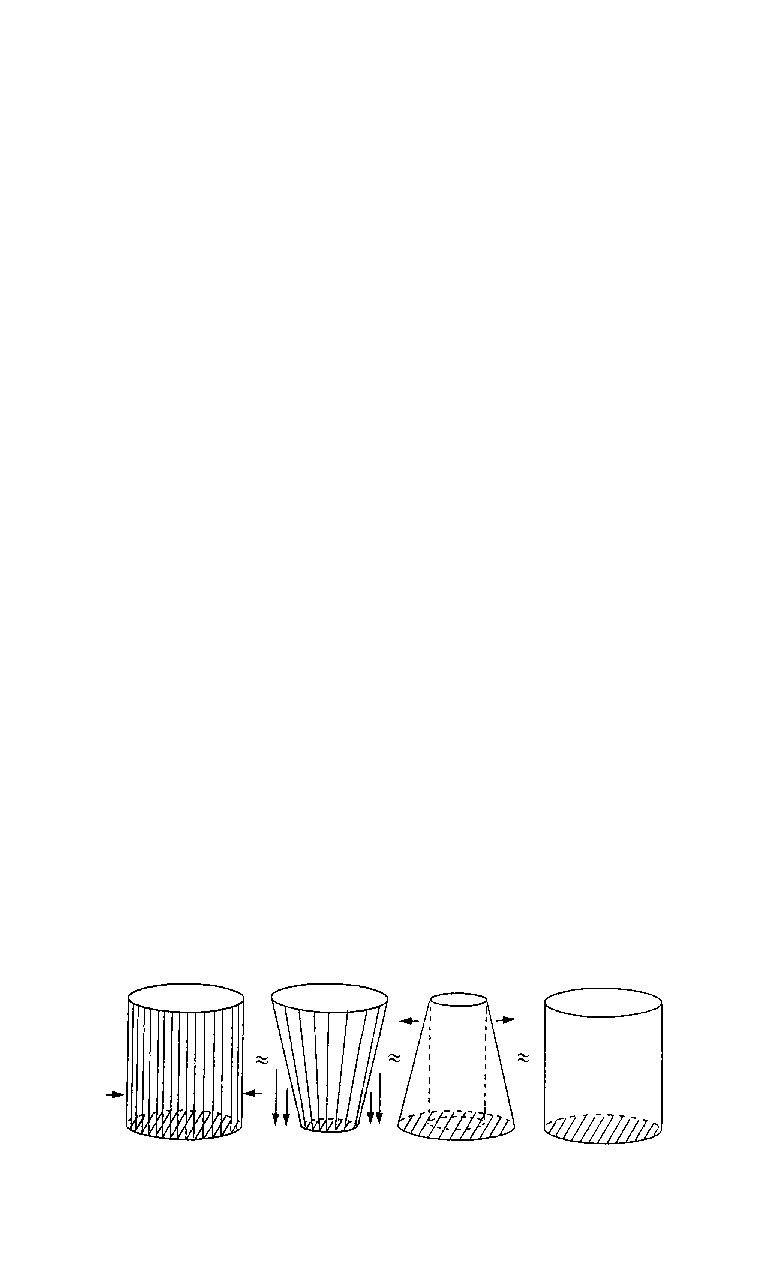
\includegraphics[width=0.5\textwidth]{figures/hom_of_pairs.pdf}
        \caption{Homeomorphism of pairs.}
        \label{fig:homeomorphism of pairs}
    \end{figure}
\end{proof}


The next Theorem shows that a map $E\to B$ that is a Serre fibration locally around each point in $B$ must be a Serre fibration. For Hurewicz fibrations the analogous statement is not generally true, i.e.~a local Hurewicz fibration is not always a Hurewicz fibration, but holds, for example, over paracompact base spaces.

\begin{thm}[{{\cite[Theorem~6.3.3]{tomDieck}}}]\label{thm local fibration}
    Let $p:E\to B$ be a continuous map and $\mathcal{U}$ a collection of subsets whose interiors cover $B$. If for every $U\in\mathcal{U}$ the restriction $p_U:p^{-1}(U)\to U$ is a Serre fibration, then so is $p$.
\end{thm}
\begin{proof}
    Subdivide the cube $I^n$ into cubes of size $\delta$ and enumerate them $I_i$. We can choose $\delta$ so that each cube $I_i\times I$ is mapped inside a $U\in\mathcal{U}$ by the map $H$ that we seek to lift. This is possible by the Lebesque Lemma~\ref{Lebesque lemma}. Let $V^k\subset I^n$ denote the union of the $k$-dimensional faces of the subdivision of $I^n$.

    We have to solve the lifting problem for the space $I^n$ with initial condition $h_0$. We begin by extending $h_0$ over $I^n\times [0,\delta]$ to a lifting of $H$. We solve the lifting problems 
     \[
    \begin{tikzcd}[every matrix/.append style={name=m}]
       I^n\times\{0\} \cup V^{k-1}\times [0,\delta] \arrow[d,"i",swap]\arrow[r,"\wt{H}(k-1)"]& E\arrow[d,"p"]\\
       I^{n}\times \{0\}\cup V^k\times [0,\delta]\arrow[r,"H",swap]\arrow[ur,"\wt{H}(k)",dashed,swap] & B
    \end{tikzcd}
    \]
    for $k=0,\ldots,n$ with $V^{-1}=\varnothing$ and $\wt{H}(-1)=a$ by induction in $k$. Let $W$ be a $k$-dimensional cube and $\partial W$ the union of its $(k-1)$-dimensional faces. We can solve the lifting problems
     \[
    \begin{tikzcd}[every matrix/.append style={name=m}]
       W\times\{0\} \cup \partial W\times [0,\delta] \arrow[d,"i",swap]\arrow[r,"\wt{H}(k-1)"]& p^{-1}(U)\arrow[d,"p_U"]\\
       W\times [0,\delta]\arrow[r,"H",swap]\arrow[ur,"\wt{H}_W",dashed,swap] & U
    \end{tikzcd}
    \]
    by a map $\wt{H}_W$, since $p_U$ is a Serre fibration; here $U\in\mathcal{U}$ was chosen such that $H(W\times [0,\delta])\subset U$.

    The $\wt{H}_W$'s for different $U\in\mathcal{U}$ combine to a continuous map $\wt{H}(k):V^l\times [0,\delta]\to E$ which covers $H$ and extends $\wt{H}(k-1)$. We define $\wt{H}$ on the first layer $I^n\times [0,\delta]$ as $\wt{H}(n)$. We now treat $I^n\times [\delta,2\delta]$ similarly with initial condition given by $\restr{\wt{H}(n)}{I^n\times\{\delta\}}$ and continue in this manner inductively.
\end{proof}

\begin{prop}[{{\cite[Prop.~3.2.3]{RS2}}}]\label{prop 3.2.3 RS2}
    Serre fibrations have the \textit{lifting property} (without homotopy) with respect to all pairs of the form
    \begin{enumerate}
        \item $(K\times I,(K\times \{0\})\cup(L\times I))$, where $K$ is a $CW$-complex and $L$ is a subcomplex. This constitutes a relative \gls{hlp} for the pair $(K,L)$.
        \item $(K,L)$ where $K$ is a $CW$-complex and $L$ is a subcomplex which is a strong deformation retract of $K$.
    \end{enumerate}
\end{prop}
\begin{proof}
    Let $\pi:E\to B$ be a Serre fibration, let $K$ be a $CW$-complex and $L$ a subcomplex of $K$.

    1. Consider the lifting problem defined by some $f:K\times I\to B$ and an initial condition $\wt{f}_0:(K\times\{0\})\cup(L\times I)\to E$. We prove the assertion by induction on the dimension $k$ of the cells attached to $L$ to build $K$. The case $k=0$ is trivial. Thus, assume we have already constructed a lifting $\wt f$ over the subspace $(K^{(k)}\cup L)\times I\subset K\times I$ for some $k\geq 0$ and consider a $(k+1)$-cell $C$ not contained in $L$ with characteristic map $\chi:\bbD^{k+1}\to K$. Since $C$ is not contained in $L$, we have $C\cap (K^{(k)}\cup L)=C\cap L^{(k)}$. Hence, we wish to extend $\wt{f}$ from 
    \[(C\times\{0\}) \cup((C\cap K^{(k)})\times I)\subset C\times I\]
    to a lifting of $f$ on $C\times I$. Assume that we can extend
    \[\wt{f}\circ \restr{(\chi\times\id_I)}{(\bbD^{k+1}\times\{0\})\cup (\partial \bbD^{k+1}\times I)}\]
    to a lifting of $f\circ (\chi\times\id_I)$ on $\bbD^{k+1}\times I$. Since $\chi $ is injective on $\Int \bbD^{k+1}$, this lifting uniquely determines a lift of $f$ on $C\times I$. By Proposition~\ref{prop 3.1.11 RS2}, applied to the $CW$-complex $C\times I$, the latter is continuous.

    This argument shows that in order to prove that $\wt f$ extends to a lifting of $f$ over $(K^{(k+1)}\cup L)\times I$, it suffices to show that $\pi$ has the relative \gls{hlp} with respect to the pair $(\bbD^{k+1},\bbS^k)$. This holds by Proposition~\ref{prop 3.2.4 tomDieck} since $\pi$ is Serre fibration.

    2. Let $F:K\times I\to K$ be a strong deformation retraction from $K$ to $L$ and consider the lifting problem defined by some $f:K\to X$ and an appropriate initial condition $\wt{f}_0:L\to E$. Define $g:K\times I\to B$ by $g=f\circ F$. Since $F$ maps subsets $K\times\{1\}$ and $L\times I$ to $L$, we can also define
    \[\wt{g}_0:(K\times\{1\})\cup(L\times I)\to E,\quad \wt{g}_0(x,t)=\wt{f}_0(F(x,t)).\]
    A brief calculation shows that $\wt{g}_0$ is a lifting of $g$ over the subset $(K\times\{1\})\cup(L\times I)$. Hence, according to point 1, it can be extended to a lift $\wt{g}$ of $g$. Then, another brief calculation shows that the mapping $\wt f:K\to E$ defined by $\wt{f}(x)=\wt{g}(x,0)$ is a lifting of $f$ through $\pi$ extending $\wt{f}_0$.
\end{proof}

\begin{thm}\label{thm 6.3.1 tomDieck}
    Let $p:E\to B$ be a Serre fibration. For $B_0\subset B$ let $E_0=p^{-1}(B_0)$. Choose basepoints $*\in B_0$ and $* \in p^{-1}(*)$. Then $p$ induces for $n\geq 1$ a bijection $p_\ast:\pi_n(E,E_0,*)\to \pi_n(B,B_0,*)$.
\end{thm}
\begin{proof}
    First we show surjectivity. Let $g \in \pi_n(B,B_0,*)$ be represented by $\gamma:(\bbD^n,\bbS^{n-1},*)\to (B,B_0,*)$.
    By \gls{hlp} there exists a lifting $\wt\gamma:\bbD^n\to E$ with $\wt\gamma(*)=*$ and $p\circ \wt\gamma=\gamma$. We then have $\wt\gamma(\bbS^{n-1})\subset E_0$ and thus $\wt\gamma$ represents a preimage pf $g$ under $p_\ast$.

    To show injectivity, let $g_0,g_1\in \pi_n(E,E_0,*)$ be represented by $\gamma_0,\gamma_1$ and have the same image under $p_\ast$. Then there exists a homotopy $\phi_t:(\bbD^n,\bbS^{n-1},*)\to (B,B_0,*)$ such that $\phi_0=p\circ \gamma_0$ and $\phi_1=p\circ \gamma_1$. Consider the subspace $T=\bbD^n\times\partial I\cup *\times I$ and define $G:T\to E$ by 
    \[G(x,t)=
        \begin{cases}
            \phi_t(x),& x\in \bbD^n, t\in\{0,1\},\\
            *, & x=*, t\in I.
        \end{cases}
    \]
    The set $T\subset \partial(\bbD^n\times I)$ is transformed into $*$ if one interchanges the last two coordinates. By \gls{hlp} again, there exists a map $H:\bbD^n\times I\to E$ such that $\restr{H}{T}=G$ and $p\circ H=\phi$. We can view $H$ as a homotopy from $\gamma_0$ to $\gamma_1$.
\end{proof}
By taking $B_0$ to be a single point, we get the following corollary, which for $n\geq 2$ is just a generalization of Corollary~\ref{cor homotopy groups of coverings} for covering spaces to all fibrations.
\begin{cor}
    Given a Serre fibration $p:E\to B$ with $F=p^{-1}(*)$, there is an isomorphism of homotopy groups
    \[\pi_n(E,F,*)\cong \pi_n(B,*),\quad n\geq 1.\]
\end{cor}
With the help of this isomorphism, we immediately get a special case of the long exact sequence of a pair (Theorem~\ref{thm long exact seq of homotopy}).
\begin{thm}[Exact sequence of a Serre fibration]\label{thm long exact sequence of serre fibration}
    For a Serre fibration $p:E\to B$ with inclusion $i:F=p^{-1}(b)\subset E$ and $e\in F$ the sequence
    \begin{multline}
        \cdots \to \pi_n(F,e)\overset{i_\ast}{\to}\pi_n(E,e)\overset{p_\ast}{\to}\pi_n(B,b)\overset{\partial}{\to}\pi_{n-1}(F,e)\to\cdots\\ 
        \to \pi_0(E,e)\to \pi_0(B,b)
    \end{multline}
    is exact.
\end{thm}

The boundary map $\partial$ has the following description. Let $f:(I^n,\partial I^n)\to (B,b)$ be given. View $f$ as a map $I^{n-1}\times I\to B$ and lift it to $\wt{f}:I^n\to E$, constant and equal to $e$ on $J^{n-1}=I^{n-1}\times \{0\}\cup \partial I^{n-1}\times I$. Then $\partial[f]$ is represented by $\restr{\wt{f}}{I^{n-1}\times \{1\}}$. In plain language, a ``loop'' representing an element of $\pi_n(B)$ in the base can be lifted to a ``path'' in the total space whose ``endpoints'' lie in the same fiber $F$, and by restricting to $F$ we get a lower-dimensional ``loop'' that represents an element of $\pi_{n-1}(F)$. The very end of the sequence requires a little extra work.

\begin{defn}[Trivialization]
    Let $\pi :E\to B$ be continuous and $U\subset B$ open and contained in the image of $\pi$. A \emph{trivialization} of $\pi$ over $U$ is a homeomorphism $\varphi:\pi^{-1}(U)\to U\times F$ over $U$, i.e., a homeomorphism which satisfies $\mathrm{pr}_1\circ \varphi=\pi$ (where $\mathrm{pr}_1$ is the natural projection onto the first component of the direct product). This condition determines $F$ up to a homeomorphism since $\varphi$ induces a homeomorphism of $\pi^{-1}(u)$ with $\{u\}\times F$.
\end{defn}

\begin{defn}[Locally trivial map]
    The map $\pi$ is \emph{locally trivial} if there exists an open covering $\mathcal{U}$ of $B$ such that $\pi$ has a trivialization over each $U_\alpha\in \mathcal{U}$. 
\end{defn}

Note that a locally trivial map is open and hence a topological quotient map.

\begin{example}
    Since a product projection is a fibration, we have by Theorem~\ref{thm local fibration} that any locally trivial map is a Serre fibration.
\end{example}
\begin{example}[Exact sequence of a covering space]
    Let $p:E\to B$ be a covering map with typical fiber $F$. Since each map $\bbD^n\to F$ must be constant because of discreteness of $F$, $\pi_n(F,*)$ is trivial for $n\geq 1$. The exact sequence of $p$ then confirms the isomorphisms $\pi_n(E,f)\cong \pi_n(B,b)$, $n\geq 2$, that we proved in Corollary~\ref{cor homotopy groups of coverings}. Moreover we have the exact sequence (omitting the common basepoint)
    \[1\to \pi_1(E)\overset{p_\ast}{\to} \pi_1(B)\overset{\partial}{\to} \pi_0(F)\overset{i_\ast}{\to} \pi_0(E)\overset{p_\ast}{\to} \pi_0(B)\to 1\]
    with the inclusion $i:F=p^{-1}(*)\subset E$ and $\pi_0(F)=F$. It yields for the universal covering $p:\bbR \to \bbS^1$ the familiar bijection $\partial:\pi_1(\bbS^1)\cong \bbZ$.
\end{example}

\begin{defn}[Hopf fibrations]\label{def: Hopf fibrations}
    Looking slightly ahead, consider $\bbS^{2n-1}\subset \bbC^n$ as a space with a free action of $\bbS^1=U(1)$ induced from scalar multiplication by $\rme^{2\pi\rmi  t}$. Let $U_j$ be the set of points $z=(z_1,\ldots,z_n)\in\bbC^n$ with $z_j\neq 0$. The map $z\mapsto z_j/|z_j|$ shows that $U_j\cong \bbR^{2n-1}\times \bbS^1$ is a trivial $U(1)$-space. The orbit space of this action is exactly $\mathbb{C}P^{n-1}=\bbS^{2n-1}\slash \bbS^1$. The Hopf fibration is defined as the orbit map $p:\bbS^{2n-1}\to \mathbb{C}P^{n-1}$. It is indeed a fibration because it is clearly trivial over $U_j\cap \bbS^{2n-1}$. We will also see a more explicit definition of the most important $n=2$ Hopf fibration later on.
\end{defn}

\begin{example}
    The exact sequence for the Hopf fibration, combined with $\pi_i(\bbS^1)=0$ for $i>1$ (see Corollary~\ref{cor: homotopy groups of circle}), yields the isomorphisms
    \[p_\ast: \pi_i(\bbS^{2n+1})\cong \pi_i(\mathbb{C}P^n),\; i\geq 3;\]
    and in particular $\pi_i(\bbS^3)\cong \pi_i(\bbS^2)$ for $i\geq 3$, since $\mathbb{C}P^1\cong \bbS^2$.
\end{example}

\begin{prop}[{{\cite[Prop.~6.3.8]{tomDieck}}}]\label{prop 6.3.8 tomDieck}
    Let $p:(E_1,E_0)\to B$ be a relative Serre fibration, i.e., $p:E_1\to B$ is a Serre fibration and the restriction $\restr{p}{E_0}$ is also a Serre fibration. Let $(F^1_b,F^0_b)$ be the pair of fibers over $p_1(e)=b\in B$. Then:
    \begin{enumerate}
        \item The inclusion induces bijections $\pi_n(F_b^1,F_b^0,e)\cong\pi_n(E_1,E_0,e)$.
        \item $\pi_0(E_0)\to \pi_0(E_1)$ is surjective iff $\pi_0(F_b^0)\to \pi_0(F_b^1)$ is surjective for each $b\in B$.
    \end{enumerate}
\end{prop}
\begin{proof}
    (1) We first prove the claim for $n=1$ and begin with surjectivity. Let $f:(I,\partial I,0)\to (E_1,E_0,e)$ be given. The path $\widebar{p\circ f}:I\to B$ (recall that the bar represents reversing the path) is lifted to $g:I\to E_0$ with initial point $f(1)$. Then $g(1)\in F^0_b$, and $f$ and $f\bullet g$ represent the same element in $\pi_1(E_1,E_0,e)$. The projection $p\circ(f\bullet g)$ is a nullhomotopic loop with basepoint $b$. We lift a nullhomotopy to $E_1$ with initial condition $f\bullet g$ on $I\times\{0\}$ and constant on $\partial I\times I$. The lifting is a homotopy $(I,\partial I,0)\times I\to (E_1,E_0,e)$ from $f\bullet g$ to a map into $(F^1_b,F^0_b,e)$. This proves the surjectivity.

    Suppose $f_0,f_1:(I,\partial I,0)\to (F^1_b,F^0_b,e)$ are given, and let $K:(I,\partial I,0)\times I\to (E_1,E_0,e)$ be a homotopy from $f_0$ to $f_1$. We lift $\widebar{p\circ K}$ to $L:I^2\to E_0$ with initial condition $L(s,0)=K(s,1)$ and $L(0,t)=L(1,t)=e$. The homotopy $p\circ(K\bullet_2 L)$ is a homotopy of loops which is $\rel \partial I^2$ homotopic to the constant map. We lift a homotopy to $E_1$ with initial condition $K\bullet_2 L$ on $I^2\times\{0\}$ and constant on $\partial I^2\times I$. The end is a homotopy from $f_0\bullet \kappa_e$ to $f_1\bullet\kappa_e$ (where $\kappa_e$ is a constant loop at $e$). This proves the injectivity.

    The higher dimensional case is obtained by an application to the relative Serre fibration $(\Omega^n F^1_b,\Omega^n F^0_b)\to (\Omega^n E_1,\Omega^nE_0)\to B$.

    (2) Suppose $\pi_0(E)\to \pi_0(E_1)$ is surjective. The argument above for surjectivity is used to show the surjectivity of $\pi_0(F^0_b)
    to \pi_0(F^1_b)$. The opposite implication is easy.
\end{proof}





\section{Higher connectivity}

For many applications it is important to know that the homotopy groups of a space vanish in a certain range. We discuss several reformulations of this fact. In the following $\pi_0(X,x_0)=\pi_0(X)$. The space $\bbD^0$ is a singleton and $\bbS^{-1}=\varnothing$.

\begin{prop}[{{\cite[Prop.~6.7.1]{tomDieck}}}]\label{prop 6.7.1 tomDieck} 
Let $n\geq 0$. \gls{tfae}:
\begin{enumerate}
    \item $\pi_n(X,x)=0$ for each $x\in X$.
    \item Each map $\bbS^n\to X$ has an extension to $\bbD^{n+1}$.
    \item Each map $\partial \bbD^{n+1}\to X$ has an extension to $\bbD^{n+1}$.
\end{enumerate}
\end{prop}
\begin{proof}
    The case $n=0$ is trivial. The equivalence of (2) and (3) is a consequence of the homeomorphism $(\bbD^{n+1},\bbS^n)\cong(I^{n+1},\partial I^{n+1})$. Suppose $f:\bbS^n\to X$ is given. Use $e_1=(1,0,\ldots)\in \bbS^n$ as a base point and think of $f$ as representing an element of $\pi_n(X,x)$. If (1) holds, then $f$ is pointed null homotopic. A null homotopy $\bbS^n\times I\to X$ factors over the quotient map $\bbS^n\times I\to \bbD^{n+1}$, $(x,t)\mapsto (1-t)e_1+tx$ and yields an extension of $f$. Conversely, let an element $\alpha$ of $\pi_n(X,x)$ be represented by a pointed map $f:(\bbS^n,e_1)\to (X,x)$. If this map has an extension $F$ to $\bbD^{n+1}$, then $(F,f)$ represents $\beta\in \pi_n(X,X,x)=0$ with $\partial\beta=\alpha$.
\end{proof}

\begin{prop}[{{\cite[Prop.~6.7.3]{tomDieck}}}]\label{prop 6.7.3 tomDieck}
    Let $n\geq 1$. The following assertions about a topological pair $(X,A)$ are equivalent:
    \begin{enumerate}[label=(\arabic*)]
        \item $\pi_n(X,A,*)=0$ for each choice of $*\in A$.
        \item Each map $f:(I^n,\partial I^n)\to (X,A)$ is as a map of pairs homotopic to a constant map.
        \item Each map $f:(I^n,\partial I^n)\to (X,A)$ is homotopic $\rel \partial I^n$ to a map into $A$.
    \end{enumerate}
\end{prop}
\begin{proof}
    $(1)\implies(2)$. Let $f:(I^n,\partial I^n)\to (X,A)$ be given. Since $J^{n-1}$ is contractible, there exists a homotopy of the restriction $f:J^{n-1}\to A$ to a constant map. Since $J^{n-1}\subset \partial I^n$ and $\partial I^n\subset I^n$ are cofibrations, $f$ is as a map of pairs homotopic to $g:(I^n,\partial I^n)\to (X,A)$ such that $g(J^{n-1})=\{a_0\}$. Since $\pi_n(X,A,a_0)=0$, the map $g:(I^n,\partial I^n,J^{n-1})\to (X,A,a_0)$ is nullhomotopic as a map of triples.

    $(2)\implies(3)$ by the compression criterion (Proposition~\ref{prop: compression criterion}).

    $(3)\implies (1)$. Let $f:(I^n,\partial I^n,J^{n-1})\to (X,A,*)$ be given. By assumption (3), $[f]$ is contained in the image of $\pi_n(A,A,*)\to \pi_n(X,A,*)$. Now use $\pi_n(A,A,*)=0$.
\end{proof}



\begin{defn}[$n$-compressible pair]\index{$n$-compressible space}
    A topological pair $(X,A)$ is called $n$-compressible if (1)-(3) in Proposition~\ref{prop 6.7.3 tomDieck} hold. More generally, we call a map $f:X\to Y$ $n$-compressible if for each commutative diagram 
    \[
    \begin{tikzcd}[every matrix/.append style={name=m}, row sep=large, column sep=large]
       \partial \bbS^{n-1} \arrow[r,"\varphi"]\arrow[d,"i",swap] & X\arrow[d,"f"]\\
       \bbD^n \arrow[r,"\Phi", swap]\arrow[ur,"\Psi",dashed,swap] & Y
    \end{tikzcd}
    \]
    there exists $\Psi:\bbD^n\to X$ such that $\restr{\Psi}{\partial \bbD^n}=\varphi$ and $f\circ \Psi\simeq \Phi$ $\rel \partial \bbD^n$ (this amounts to (3) of Proposition~\ref{prop 6.7.3 tomDieck}). This notion is invariant under compositions with homotopy equivalences of the target space $Y$.
\end{defn}

\begin{prop}[{{\cite[Prop.~6.7.5]{tomDieck}}}]\label{prop 6.7.5 tomDieck}
    Let $n\geq 0$. The following assertions about a pair $(X,A)$ are equivalent:
    \begin{enumerate}
        \item Each map $f:(\bbD^q,\partial \bbD^q)\to (X,A)$, $q\in (0,\ldots,n)$ is $\rel \partial \bbD^q$ homotopic to a map into $A$.
        \item The inclusion $j:A\hookrightarrow X$ induces for each basepoint $a\in A$ a bijection $j_\ast:\pi_q(A,a)\to \pi_q(X,a)$ for $q<n$ and a surjection for $q=n$.
        \item $\pi_q(X,A,a)=0$ for $q=1,\ldots,n$ and each $a\in A$, and $\pi_0(A)\to \pi_0(X)$ is surjective.
    \end{enumerate}
\end{prop}
\begin{proof}
    $(1)\Leftrightarrow (3)$. The surjectivity of $\pi_0(A)\to \pi_0(X)$ is equivalent to (1) for $q=0$. The other cases follow from Proposition~\ref{prop 6.7.3 tomDieck}.

    $(2)\Leftrightarrow(3)$ follows from the exact sequence of the pair (Theorem~\ref{thm long exact seq of homotopy}).
\end{proof}


\begin{defn}[$n$-connected pair]\index{$n$-connected pair}
    A topological pair $(X,A)$ is called $n$-connected if (1)-(3) in Proposition~\ref{prop 6.7.5 tomDieck} hold. We call $(X,A)$ $\infty$-connected if the pair is $n$-connected for each $n$. A pair is $\infty$-connected iff $j_\ast:\pi_n(A,a)\to \pi_n(X,a)$ is always bijective. If $X\neq\varnothing$ but $A=\varnothing$ we say that $(X,A)$ is $(-1)$-connected, and $(\varnothing,\varnothing)$ is $\infty$-connected.
\end{defn}

\begin{defn}[Cone]\index{Cone}
    Given a space $X$, its cone $CX$ is defined as result of attaching the cylinder $X\times [0,1]$ by its face $X\times\{0\}$ to a point $*$ along the projection $p:X\times \{0\}\to *$.
\end{defn}


\begin{prop}[{{\cite[Prop.~6.7.6]{tomDieck}}}]\label{prop 6.7.6 tomDieck}
    Let $n\geq 0$. The following assertions about a space $X$ are equivalent:
    \begin{enumerate}
        \item $\pi_q(X,x)=0$ for $0\leq q\leq n$ and $x\in X$.
        \item The pair $(CX,X)$ is $(n+1)$-connected.
        \item Each map $f:\partial I^q\to X$, $0\leq q\leq n+1$ has an extension to $I^q$.
    \end{enumerate}
\end{prop}
\begin{proof}
    The cone $CX$ is contractible, therefore $\partial:\pi_{q+1}(CX,X,*)\cong \pi_q(X,*)$. This and Proposition~\ref{prop 6.7.5 tomDieck} shows the equivalence of (1) and (2). The equivalence of (1) and (3) is based on Proposition~\ref{prop 6.7.1 tomDieck}.
\end{proof}

\begin{defn}[$n$-connected space]\index{$n$-connected space}
    A space $X$ is called $n$-connected if (1)-(3) in Proposition~\ref{prop 6.7.6 tomDieck} hold. Note that this is compatible with previous definitions for $n=0$ (path-connected) and $n=1$ (simply-connected).
\end{defn}

\begin{defn}[$n$-equivalence]\index{$n$-equivalence}\index{Weak equivalence}
    Let $f:X\to Y$ be a map and $X\subset Z_f$ the inclusion into the mapping cylinder (recall the definition in Figure~\ref{fig:mapping cyl}). Then $f$ is said to be $n$-connected if $(Z_f,X)$ is $n$-connected. We then also say that $f$ is an $n$-equivalence. Thus $f$ is $n$-connected iff $f_\ast:\pi_q(X,x)\to \pi_q(Y,f(x))$ is for each $x\in X$ bijective for $q<n$ and surjective for $q=n$. If $f$ is an $\infty$-equivalence we also call it a weak (homotopy) equivalence, which happens iff $f_\ast$ is bijective for all $x\in X$ in all degrees.
\end{defn}

\begin{prop}[{{\cite[Prop.~6.7.7]{tomDieck}}}]\label{prop 6.7.7 tomDieck}
    Let $p:(E_1,E_0)\to B$ be a relative Serre fibration (see Proposition~\ref{prop 6.3.8 tomDieck}). Let $(F^1_b,F^0_b)$ be the pair of fibers over $b\in B$. Then the pair $(E_1,E_0)$ is $n$-connected iff the pairs $(F^1_b,F^0_b)$ are $n$-connected for all $b\in B$.
\end{prop}
\begin{proof}
    This is a direct consequence of Proposition~\ref{prop 6.3.8 tomDieck}.
\end{proof}

\begin{thm}[{{\cite[Theorem~6.7.9]{tomDieck}}}]\label{thm 6.7.9 tomDieck}
    Let $\varphi:(X,X_0,X_1)\to (Y,Y_0,Y_1)$ be a map such that the restrictions $\varphi_i:X_i\to Y_i$ are $n$-connected and $\varphi_{01}:X_0\cap X_1\to Y_0\cap Y_1$ is $(n-1)$-connected. Suppose $X=X_0^\circ \cup X_1^\circ$ and $Y=Y_0^\circ \cup Y_1^\circ$ where $\ ^\circ$ denotes interiors. Then $\varphi $ is an $n$-equivalence.
\end{thm}

\begin{cor}[{{\cite[Prop.~6.7.10]{tomDieck}}}]\label{prop 6.7.10 tomDieck}
    Let $f:X\to Y$ be an $n$-connected map between spaces with nondegenerate basepoints. Then the suspension $\Sigma f:\Sigma X\to \Sigma Y$ is $(n+1)$-connected. If $X$ is $n$-connected, then $\Sigma X$ is $(n+1)$-connected. The sphere $\bbS^{k+1}$ is $k$-connected.
\end{cor}
\begin{proof}
    Let $\Sigma 'X$ denote the unpointed suspension of $X$. This is a quotient of $X\times I$ and covered by the open cones $C_0=X\times [0,1)\slash X\times\{0\}$ and $C_1=X\times (0,1]\slash X\times\{1\}$ with intersection $X\times (0,1)$. We can apply Proposition~\ref{prop 6.7.7 tomDieck} directly; the cones are contractible and therefore the induced maps $C_j(X)\to C_j(Y)$ are $\infty$-connected. In the case of a space $X$ with a nondegenerate basepoint the quotient map $\Sigma 'X\to \Sigma X$ is a homotopy equivalence.
\end{proof}

\begin{thm}[{{\cite[Theorem~6.7.11]{tomDieck}}}]\label{thm 6.7.11 tomDieck}
    Let $f:X\to Y$ be a continuous map. Let $\{U_j\}_j$ and $\{V_j\}_j$ be open coverings of $X$ and $Y$ such that $f(U_j)\subset V_j$. Suppose that for each finite subset of indices the induced map $f_J:\bigcap_{j\in J}U_j\to \bigcap_{j\in J}V_j$ is a weak equivalence. Then $f$ is a weak equivalence.
\end{thm}
\begin{proof}
    By passage to the mapping cylinder we can assume that $f$ is an inclusion. Let $h:(I^n,\partial I^n)\to (Y,X)$ be given. We have to deform $h$ $\rel \partial I^n$ into $X$. By compactness of $I^n$ is suffices to work with finite coverings. A simple induction reduces the problem to a covering by only two sets $j=0,1$. Then we apply Theorem~\ref{thm 6.7.9 tomDieck}.
\end{proof}






\section{Excision for homotopy groups}

The following fundamental theorem, which we provide without proof, is an advanced relative of the Seifert-van~Kampen Theorem~\ref{thm seifert-van kampen}. While the latter allowed us to compute fundamental groups of ``composite'' spaces as free products of simpler pieces, this theorem indicates that a similar procedure for higher homotopy groups does not exist. In fact, the best case scenario is that if the pieces are sufficiently connected in low dimensions, then the composite space will inherit the homotopy groups up to some dimension. This is why it is commonly said that ``excision fails in homotopy'', unlike in homology.

\begin{thm}[Blakers-Massey excision theorem {{\cite[Thm~6.4.1]{tomDieck}}}]
    Let $X=U_0\cup U_1$ be covered by two open subspaces $U_0$ and $Y_1$ with non-empty intersection $V=U_0\cap U_1$. Suppose that $(U_0,V)$ is $p$-connected and $(U_1,V)$ is $q$-connected, i.e.
    \[
    \begin{matrix}
        \pi_i(U_0,V,*)=0,\quad 1\leq i\leq p,\; p\geq 0,\\
        \pi_i(U_1,V,*)=0,\quad 1\leq i\leq q,\; q\geq 0
    \end{matrix}
    \]
    for each basepoint $*\in V$. Then the \emph{excision map}, induced by the inclusion,
    \[i_\ast : \pi_n(U_1,V,*)\to \pi_n(X,U_0,*)\]
    is an isomorphism for $1\leq n <p+q$ and surjective for $n=p+q$ (for each $*\in X)$. In the case $p=0$, there is no condition on $\pi_i(U_0,V,*)$.
\end{thm}

\begin{cor}[{{\cite[Prop.~6.4.2]{tomDieck}}}]\label{prop 6.4.2 tomDieck}
    If in the above $(U_1,V)$ is $q$-connected then $(X,U_0)$ is $q$-connected.
\end{cor}
\begin{proof}
    This is a special case of the excision theorem which also directly follows from Theorem~\ref{thm 6.7.9 tomDieck}.
\end{proof}

For the sphere $\bbS^n$, introduce the following hemispheres and punctured spheres
\[\bbD^n_\pm=\{x\in \bbS^n\subset \bbR^{n+1}\mid \pm x_{n+1}\geq 0\}\subset H^n_\pm=\{x\in \bbS^n\mid x\neq \pm e_{n+1}\}.\]
We use the equatorial point $*=-e_1$ as a basepoint.

\begin{lem}[{{\cite[Lemma~6.4.3]{tomDieck}}}]\label{lem 6.4.3 tomDieck}
   There are isomorphisms $\partial:\pi_{i+1}(D_-^{n+1},\bbS^n,*)\to \pi_i(\bbS^n,*)$ for $i\geq 0$, $n\geq 0$ and $\pi_i(\bbS^n,*)\to \pi_i(\bbS^n,D_\pm^n,*)$ for $i\geq 0$, $n\geq 1$.
\end{lem}
\begin{proof}
    In the first case we use the exact sequence of the pair $(\bbD^{n+1}_-,\bbS^n)$. The space $\bbD^{n+1}_-$ is contractible and hence $\pi_i(\bbD^{n+1}_-,*)=0$ for $i\geq 0$ and $n\geq 0$.

    In the second case we consider similarly the exact sequence of $(\bbS^n,\bbD^n_\pm)$. Note that $*=-e_1\in D_\pm^n$ for $n\geq 1$.
\end{proof}

Thus for $n\geq 0$ we have a diagram with the isomorphisms 
\[
    \begin{tikzcd}[every matrix/.append style={name=m}, row sep=large, column sep=large]
       \pi_i(\bbS^n,*) \arrow[r,"E"] & \pi_{i+1}(\bbS^{n+1},*)\arrow[d,"\cong"]\\
       \pi_{i+1}(\bbD^{n+1}_-,\bbS^n,*)\arrow[u,"\overset{\partial}{\cong}",swap] \arrow[r,"i_\ast", swap] & \pi_{i+1}(\bbS^{n+1},D_+^{n+1},*).
    \end{tikzcd}\label{3795}
\]
The morphism $i_\ast$ is induced by the inclusion and $E$ is defined so as to make the diagram commutative. Note that the inductive proof of item 1 in the next theorem uses only Corollary~\ref{prop 6.4.2 tomDieck}.

\begin{thm}[{{\cite[Thm~6.4.4]{tomDieck}}}]\label{thm 6.4.4 tomDieck}
    \begin{enumerate}
        \item $\pi_i(\bbS^n)=0$ for $i<n$ (recall that we already showed this in Corollary~\ref{cor pi_n(S^k)=0}).
        \item The homomorphism $i_\ast$ in diagram (\ref{3795}) is an isomorphism for $i\leq 2n-2$ and an epimorphism for $i=2n-1$. A similar statement holds for $E$.
    \end{enumerate}
\end{thm}
\begin{proof}
    Let $N(n)$ be the statement (1) and $E(n)$ be the statement (2). Obviously $N(1)$ holds. Assume $N(n)$ holds. We then deduce $E(n)$. We apply the excision theorem to $(X,U_0,U_1,V)=(\bbS^{n+1},D_+^{n+1},D_-^{n+1},\bbS^n)$. By $N(n)$ and Lemma~\ref{lem 6.4.3 tomDieck} we have $\pi_i(\bbS^n)\cong \pi_{i+1}(D_\pm^{n+1},\bbS^n)=0$ for $0\leq i <n$. We use the excision theorem for $p=q=n$ and see that $i_\ast$ is surjective for $i+1\leq 2n$ and bijective for $i+1\leq 2n-1$. Finally, $E(n)$ and $N(n)$ imply $N(n+1)$.

    In order to have the correct hypotheses for the excision theorem, we thicken the spaces, replace $D_\pm^n$ by $H^n_\pm$ and note that the inclusions $D_\pm^n\subset H^n_\pm$ and $\bbS^{n-1}\subset H^n_+\cap H^n_-$ are homotopy equivalences.
\end{proof}
\begin{cor}[{{\cite[Prop.~5.11]{Bredon}}}] 
    The pair $(\bbD^{n+1},\bbS^n)$ is $n$-connected.
\end{cor}
\begin{proof}
    This follows from the exact sequence $\pi_r(\bbD^{n+1})\to \pi_r(\bbD^{n+1},\bbS^n)\to \pi_{r-1}(\bbS^n)$ for $r\leq n$, where the two groups on the sides vanish.
\end{proof}


\begin{prop}[{{\cite[Prop.~6.4.5]{tomDieck}}}]\label{prop 6.4.5 tomDieck}
    The homomorphism $\pi_i(\bbD^{n+1},\bbS^n,*)\to \pi_i(\bbD^{n+1}\slash \bbS^n,*)$ induced by the quotient map is an isomorphism for $i\leq 2n-1$ and an epimorphism for $i=2n$.
\end{prop}
\begin{proof}
    Consider the commutative diagram
    \[
    \begin{tikzcd}[every matrix/.append style={name=m}, row sep=large, column sep=large]
       \pi_i(D_-^{n+1},\bbS^n,*) \arrow[r]\arrow[d,"i_\ast",swap] & \pi_i(D_-^{n+1}\slash \bbS^n,*) \arrow[d,"(1)"]\\
       \pi_{i+1}(\bbS^{n+1},\bbD^{n+1}_+,*)\arrow[r,"(2)",swap] & \pi_{i}(\bbS^{n+1}\slash D_+^{n+1},*).
    \end{tikzcd}
    \]
    The map (1) is induced by a homeomorphism and the map (2) by a homotopy equivalence, hence both are isomorphisms. Now apply Theorem~\ref{thm 6.4.4 tomDieck}.
\end{proof}

The homomorphism $E$ is essentially the suspension homomorphism:
\[\Sigma_\ast: \pi_n(X)\underset{\cong}{\overset{\partial}{\leftarrow}}\pi_{n+1}(CX,X)\overset{q_\ast}{\to}\pi_{n+1}(CX\slash X)=\pi_{n+1}(\Sigma X)\]
with the quotient map $q:\bbD^{n+1}\to \bbS^{n+1}=\bbD^{n+1}\slash \bbS^n$. The next result is the famous suspension theorem of Freudenthal.

\begin{thm}[Freudenthal's suspension theorem {{\cite[Theorem~6.4.6]{tomDieck}}}]\label{thm 6.4.6 tomDieck freudenthal}
    The suspension $\Sigma_\ast:\pi_i(\bbS^n)\to \pi_{i+1}(\bbS^{n+1})$ is an isomorphism for $i\leq 2n-2$ and an epimorphism for $i=2n-1$.
\end{thm}
\begin{proof}
    We have to show that $q_\ast:\pi_{i+1}(CX,X)\to \pi_{i+1}(CX\slash X)$ is for $X=\bbS^n$ an isomorphism (epimorphism) in the appropriate range. This follows from Proposition~\ref{prop 6.4.5 tomDieck}; one has to use that  $\bbD^{n+1}_-$ is the (pointed) cone on $\bbS^n$.
\end{proof}

\begin{thm}[{{\cite[Theorem~6.4.7]{tomDieck}}}]\label{thm 6.4.7 tomDieck freudenthal}
    $\pi_n(\bbS^n)\cong \bbZ$ and $\Sigma_\ast:\pi_n(\bbS^n)\to \pi_{n+1}(\bbS^{n+1})$ is an isomorphism ($n\geq 1$). The group $\pi_n(\bbS^n)$ is generated by the identity map of $\bbS^n$.
\end{thm}
\begin{proof}
    From the exact sequence of the Hopf fibration $\pi_2(\bbS^3)\to \pi_2(\bbS^2)\to \pi_1(\bbS^1)\to \pi_1(\bbS^3)$ and $\pi_j(\bbS^3)=0$ for $j=1,2$, we obtain an isomorphism $\partial:\pi_2(\bbS^2)\to \pi_1(\bbS^1)\cong \bbZ$. From Theorem~\ref{thm 6.4.6 tomDieck freudenthal} we obtain a surjection $\Sigma_\ast:\pi_1(\bbS^1)\to \pi_2(\bbS^2)$; this is an isomorphism, since both groups are isomorphic to $\bbZ$. For $n\geq 2$, Theorem~\ref{thm 6.4.6 tomDieck freudenthal} directly gives an isomorphism $\Sigma_\ast$. We know that $\pi_1(\bbS^1)$ is generated by the identity map, and $\Sigma_\ast$ respects the identity.
\end{proof}

This proof clearly extends to two cones over any space $X$, so by using the adjunction $[\Sigma X,Y]\cong[X,\Omega Y]$ we get the more general form of this Theorem.

\begin{thm}[Freudenthal's suspension theorem {{\cite[Thm.~6.4.6]{tomDieck}}}]\index{Theorem!Freudenthal's suspension}
Let $X$ be an $n$-connected space, i.e., $\pi_i(X)=0$ for $0\leq i\leq n$. Then the homomorphism $\pi_k(X)\to \pi_k(\Omega \Sigma X)$ induced by the inclusion $X\hookrightarrow \Omega\Sigma X$ is an isomorphism for $k\leq 2n-2$ and an epimorphism for $k=2n-1$.

Furthermore, since $\pi_{k+1}(\Sigma X)\cong[\bbS^{k+1};\Sigma X]\cong[\bbS^k;\Omega \Sigma X]\cong\pi_k(\Omega \Sigma X)$, for $k\leq 2n-2$ there is an isomorphism $\pi_k(X)\cong \pi_{k+1}(\Sigma X)$.
\end{thm}

Since $\id_{\bbS^n}$ generates the $n$-th homotopy group of $\bbS^n$, this allows us to make the following definition.

\begin{defn}[Degree on spheres]\index{Degree}
    For a map $f:\bbS^n\to \bbS^n$, its degree $\deg f$ is the integer such that $[f]=[\mathrm{id}_{\bbS^n}]^{\deg f}$ in $\pi_n(\bbS^n)$.
\end{defn}

\begin{example}[Hopf fibrations]\label{example Hopf pi3(S2)}
    We continue the discussion of the Hopf fibrations \ref{def: Hopf fibrations}. The Hopf fibration $\bbS^{2n+1}\to \mathbb{C}P^n$ and $\pi_i(\bbS^{2n+1})=0$ for $i\leq 2n$ yield $\pi_2(\mathbb{C}P^n)\cong \pi_1(\bbS^1)\cong \bbZ$ and $\pi_i(\mathbb{C}P^n)=0$ for $0\leq i \leq 2n$, $i\neq 2$. The inclusion $\bbS^{2n+1}\to \bbS^{2n+3}$, $z\mapsto (z,0)$ induces an embedding $\mathbb{C}P^n\subset \mathbb{C}P^{n+1}$. We compare the corresponding Hopf fibrations and their exact sequences and conclude $\pi_2(\mathbb{C}P^n)\cong \pi_2(\mathbb{C}P^{n+1})$. Let $\mathbb{C}P^\infty =\bigcup_{n\geq 1}\mathbb{C}P^n$ be the colimit (the topology on it is defined as the finest topology under which all inclusions $\mathbb{C}P^n\hookrightarrow \mathbb{C}P^\infty$ are continuous). The inclusions induce $\pi_i(\mathbb{C}P^n)\cong\pi_i(\mathbb{C}P^\infty)$ for $i\leq 2n$. A proof uses the fact that a compact subset of $\mathbb{C}P^\infty$ is contained in some finite $\mathbb{C}P^N$. Therefore $\mathbb{C}P^\infty$ is a space with a single nontrivial homotopy group $\pi_2(\mathbb{C}P^\infty)\cong\bbZ$.

    Particularly notable is the special case 
    \[\pi_3(\bbS^2)\cong \pi_3(\bbS^3)\cong\bbZ.\]
    This is the first of the ``nontrivial'' homotopy groups of spheres $\pi_k(\bbS^n), k>n$, and the only one that can be computed without much more advanced homology theory.

    We have the similar results for real projective spaces. The double coverings $\bbS^n\to \RP^n$ are used to show that $\pi_1(\RP^2)\cong \pi_1(\RP^3)\cong\cdots =\cong \pi_1(\RP^\infty)\cong \bbZ_2$, induced by the inclusions $\RP^n\hookrightarrow\RP^{n+1}$ for $i<n$ and $\pi_i(\RP^n)=0$ for $0\leq i< n$, $i\neq 1$. The space $\RP^\infty$ therefore has a single nontrivial homotopy group $\pi_1(\RP^\infty)\cong\bbZ_2$.
\end{example}


\begin{example}[Lens spaces]\index{Lens spaces}
    Recall the lens space $L=L_m(l_1,\ldots,l_n)$ from Example~\ref{example Lens spaces}. It can be given a structure of a $CW$-complex with one cell in each dimension from $0$ to $2n-1$ so that the degree of the attaching maps alternates between $0$ and $m$ (starting with degree $0$ for the map $\partial \bbD^1\to L^{(0)}$).
\end{example}


\begin{example}[$\pi_3(\bbS^2\vee \bbS^2)\cong \bbZ^3$]
    Let us compute $\pi_3(\bbS^2\vee \bbS^2)$. We have an inclusion $i: \bbS^2\vee \bbS^2\hookrightarrow \bbS^2\times \bbS^2$, because $\bbS^2\times \bbS^2$ can be realized as a $CW$-complex that differs from $\bbS^2\vee \bbS^2$ only by an addition of a 4-cell. Observe that the induced homomorphism on the homotopy groups is surjective:
    \[i_\ast: \quad \pi_n(\bbS^2\vee \bbS^2)\to \pi_n(\bbS^2\times \bbS^2)=\pi_n(\bbS^2)\oplus \pi_n(\bbS^2).\]
    (Here we used the fact that a smash product with $\bbS^k$ is homeomorphic to the iterated reduced suspension $\Sigma^k$, and $\Sigma^k \bbS^n=\cong \bbS^{n+k}$.) This allows us to insert extra zeroes into the long exact sequence for the pair $(\bbS^2\times \bbS^2,\bbS^2\vee \bbS^2)$ without breaking its exactness, which splits it into the short exact sequences
    \[0\to \pi_{n+1}(\bbS^2\times \bbS^2,\bbS^2\vee \bbS^2)\to \pi_n(\bbS^2\vee \bbS^2)\overset{i_\ast}{\to} \pi_n(\bbS^2\times \bbS^2)\to 0.\]
    For $n=3$, since $\bbS^2\vee \bbS^2$ is 1-connected and the remaining 4-cell is 4-connected, we can use the excision theorem to compute
    \[\pi_4(\bbS^2\times \bbS^2,\bbS^2\vee \bbS^2)\cong \pi_4(\bbS^2\times \bbS^2\slash \bbS^2\vee \bbS^2)\cong \pi_4(\bbS^2\wedge \bbS^2) \cong\pi_4(\bbS^4)\cong \bbZ.\]
    At the same time, $\pi_3(\bbS^2\times \bbS^2)=\pi_3(\bbS^2)\oplus \pi_3(\bbS^2)=\bbZ^2$ (generated by the Hopf fibrations from the preceding Example~\ref{example Hopf pi3(S2)}). Thus we have the exact sequence
    \[0\to \bbZ\to \pi_3(\bbS^2\vee \bbS^2)\to \bbZ^2\to 0,\]
    which implies $\pi_3(\bbS^2\vee \bbS^2)=\bbZ^3$ because every short exact sequence of the form $0\to A\overset{i}{\to} B\overset{p}{\to} \bbZ^2\to 0$ splits (the splitting monomorphism $j:\bbZ^2\to B$ can be constructed by defining it on the basis $j(1,0)=b_1$ and $j(0,1)=b_2$, where $b_1,b_2\in B$ are any two elements such that $p(b_1)=(1,0)$ and $p(b_2)=(0,1)$; it is then easy to check that $p\circ j=\id_{\bbZ^2}$ and hence $B\cong A\oplus \bbZ^2$).

    This construction is a special case of the \emph{Whitehead product}\index{Whitehead product} $\pi_k(X)\times\pi_l(X)\to \pi_{k+l-1}(X)$. Given $f:\bbS^k\to X$ and $g:\bbS^l\to X$, their Whitehead product is the homotopy class denoted
    \[[f,g]\in \pi_{k+l-1}(X)\]
    and represented by the composition 
    \[\bbS^{k+l-1}\overset{\chi}{\to} \bbS^k\vee \bbS^l\overset{f\vee g}{\to} X,\]
    where $\chi$ is the attaching map for the single $(k+l)$-cell in the $CW$-complex $\bbS^k\times \bbS^l$ which consists of $\bbS^k\vee \bbS^l$ and that cell ($\chi$ maps the boundary of the $(k+l)$-disk to the $(k+l-1)$-skeleton, which in this case is $\bbS^k\vee \bbS^l$). In the case above, the third ``unexpected'' generator of $\pi_3(\bbS^2\vee \bbS^2)$ is $[i_1,i_2]$, where $i_1,i_2:\bbS^2\to \bbS^2\vee \bbS^2$ are the inclusion maps for the two 2-spheres. 
    
    Another simple Whitehead product is $[\id_{\bbS^2},\id_{\bbS^2}]\in\pi_3(\bbS^2)$. It is represented by the map obtained by gluing $\bbS^2\vee \bbS^2\subset \bbS^3$ onto $\bbS^2$. Since we already know that $\pi_3(\bbS^2)$ is generated by the Hopf fibration $p_{\mathrm{Hopf}}$ and this map clearly has winding number $2$, we find that 
    \[[\id_{\bbS^2},\id_{\bbS^2}]=2[p_{\mathrm{Hopf}}]\]
    (although there might also be a minus sign depending on how one defines the Hopf fibration).
\end{example}

\begin{xca}[{{\cite[Thm.~6.10.5]{tomDieck}}}]
    Let $X$ and $Y$ be well-pointed (i.e.~with non-degenerate basepoints) and assume that $\pi_i(X)=\pi_j(Y)=0$ for $i<p,j<q$ with $p,q\geq 2$. Show that the inclusion $X\vee Y\hookrightarrow X\times Y$ induces an isomorphism of the $\pi_i$-groups for $i\leq p+q-2$. Also show that $\pi_i(X\times Y,X\vee Y)$ and $\pi_i(X\wedge Y)$ vanish for $i\leq p+q-1$.
\end{xca}

\begin{xca}[{{\cite[Exercise 6.11]{tomDieck}}}]
    Extend the above example to determine $\pi_{2n-1}(\bbS^n\vee \bbS^n)$ for $n\geq 2$.
\end{xca}

